%%-------------------------------------------------------------------------------------------------
%%                           Template Notes:
%% Make sure to have all template files from klmweb/revisions/templates/JJH_Beamer before using
%% this file. Also please read the Beamer Reference document for typists if you have any questions
%% on the usage of this template.
% -------------------------------------------------------------------------------------------------
\documentclass[static]{JJH-Beamer}

%% -- Extra Packages (Place Packages here if they are not included in the default template)--------

\usepackage{booktabs}
\usepackage{soul}
\usepackage{tabularx}
\usepackage{graphicx}
\usepackage{colortbl}
\usepackage[para]{threeparttable}
\usepackage{epstopdf}
\usepackage{subfig}
\usepackage{bbding}
\usepackage{appendixnumberbeamer}
\usepackage{rotating}
\usepackage{geometry}
\usepackage{pdflscape}
\usepackage{setspace}

%% ------ Extra Preamble Definitions (Place any other extra preamble stuff here) ------------------


\newcommand{\mr}{\multirow}
\newcommand{\mc}{\multicolumn}
\newcolumntype{L}[1]{>{\raggedright\let\newline\\\arraybackslash\hspace{0pt}}m{#1}}
\newcolumntype{C}[1]{>{\centering\let\newline\\\arraybackslash\hspace{0pt}}m{#1}}
\newcolumntype{R}[1]{>{\raggedleft\let\newline\\\arraybackslash\hspace{0pt}}m{#1}}

\newtheorem{claim}{Claim}
\newtheorem{condition}{Condition}
\renewcommand\thecondition{C--\arabic{condition}}
\newtheorem{algorithm}{Algorithm}
\newtheorem{assumption}{Assumption}
\renewcommand\theassumption{A--\arabic{assumption}}
\newtheorem{hypothesis}[theorem]{Hypothesis}

\newcommand\independent{\protect\mathpalette{\protect\independenT}{\perp}}
\def\independenT#1#2{\mathrel{\rlap{$#1#2$}\mkern2mu{#1#2}}}
\newcommand{\overbar}[1]{\mkern 1.5mu\overline{\mkern-1.5mu#1\mkern-1.5mu}\mkern 1.5mu}
\newcommand{\equald}{\ensuremath{\overset{d}{=}}}
\captionsetup[table]{skip=10pt}

\newcommand{\backupbegin}{
   \newcounter{finalframe}
   \setcounter{finalframe}{\value{framenumber}}
}
\newcommand{\backupend}{
   \setcounter{framenumber}{\value{finalframe}}
}

\newcommand*\leftright[2]{%
  \leavevmode
  \rlap{#1}%
  \hspace{0.5\linewidth}%
  #2}

%Other parameters
\newcommand{\noutcomes}{95}
\newcommand{\noutcomesexpp}{357}
\newcommand{\noutcomesexpm}{343}
\newcommand{\noutcomesexpf}{355}
\newcommand{\treatsubsabc}{$75\%$}
\newcommand{\treatsubscarec}{$74\%$}
\newcommand{\treatsubscaref}{$63\%$}

%Counts
%Males
\newcommand{\positivem}{$78\%$}
\newcommand{\positivesm}{$29\%$}

%Females
\newcommand{\positivef}{$78\%$}
\newcommand{\positivesf}{$31\%$}

%Counts, control substitution
%Males
\newcommand{\positivecsnm}{$47\%$}
\newcommand{\positivescsnm}{$15\%$}

\newcommand{\positivecsam}{$79\%$}
\newcommand{\positivescsam}{$29\%$}

%Females
%% no alternative
\newcommand{\positivecsnf}{$84\%$}
\newcommand{\positivescsnf}{$55\%$}

%% alternative
\newcommand{\positivecsaf}{$79\%$}
\newcommand{\positivescsaf}{$33\%$}

%Pooled

%Effects
%Males

%Females
\newcommand{\empf}{$8$}
\newcommand{\yearsedf}{$1.7$}



%Pooled

%CBA
%IRR
%Males
\newcommand{\irrm}{$15\%$}
\newcommand{\irrsem}{$5\%$}

%Females
\newcommand{\irrf}{$9\%$}
\newcommand{\irrsef}{$7\%$}

%Pooled
\newcommand{\irrp}{$13\%$}
\newcommand{\irrsep}{$5\%$}

%BC
%Males
\newcommand{\bcm}{$11.24$}
\newcommand{\bcsem}{$4.60$}

%Females
\newcommand{\bcf}{$2.35$}
\newcommand{\bcsef}{$1.09$}

%Pooled
\newcommand{\bcp}{$5.63$}
\newcommand{\bcsep}{$2.15$}

%NPV streams
%Pooled
\newcommand{\parincomenpvp}{$\$119,346$}

% ------------ Title, author, date (ALWAYS UPDATE THESE THINGS) -----------------------------------

\def \thetitle {The Life-cycle Benefits of an Influential Early Childhood Program} % Full title goes here

\def \theshorttitle {Life-cycle Benefits, Early Childhood Program} %Short title goes here

\def \theauthor {Jorge Luis Garc\'{i}a, James J. Heckman,\\ Duncan Ermini Leaf, Mar\'{i}a Jos\'{e} Prados} % Author name(s) go here

\def \theshortauthor {Garc\'{i}a et al.} % Short author name(s) go here; should fit on this one line.

\def \thedate {University of Wisconsin-Madison \\ Department of Economics\\
Public Workshop\\
February 27th, 2016} % Date and venue information

\def \eventnotes {\noindent
\textbf{Date:} Monday, February 27th, 2016\\
\textbf{Event Title:} Public Workshop --- UW-Madison\\
\textbf{Host:} Professor Matt Wiswall\\
\textbf{Location:} Economics Department\\
\textbf{Presentation Title:} The Life-Cycle Benefits of an Influential Early Childhood Program\\
\textbf{Format:} Presentation\\
\textbf{Length:} 90 minutes\\
\textbf{Time:} 3:30 pm -- 5:00 pm\\
\textbf{Audience Background:} Faculty and students.\\
\textbf{Additional Information:}\\

} % Other event info, to appear on the front of the private notes

% -------------------------------------------------------------------------------------------------

\begin{document}
%\renewcommand*{\inserttotalframenumber}{\pageref{lastframe}}

\mode<all>{\theTitlePages} % Macro to insert both title pages DO NOT REMOVE!

%%
%% ------------------------- Content starts here --------------------------------------------------
\begin{frame}

\begin{center}
\textbf{Subject of Analysis:}
\end{center}

\begin{itemize}
\item Prototypical early childhood education program(s), treating children from ages 0 to 5
\end{itemize}

\begin{center}
\textbf{Goal of Paper:}
\end{center}

\begin{itemize}
\item An economic evaluation of a prototypical and influential early childhood program that attempted to build lasting skills

\begin{center}
\textbf{How?}
\end{center}
\item Combine datasets to predict life-cycle benefits and costs
\item Estimate benefit/cost ratio and rate of return of program accounting for its multiple benefits
\end{itemize}

\end{frame}

%% ------------------------- Content starts here --------------------------------------------------
\begin{frame}
\frametitle{Roadmap}

\begin{enumerate}
\item Introduce challenges, describe the program, survey results
\item Give more details on the program
\item Present evaluation framework and parameters of interest
\item \textbf{Middle step:} what are the treatment effects?
\item Predict and monetize life-cycle benefits and costs
\item Put it all together: B/C ratio and IRR
\item Summary
\end{enumerate}

\end{frame}


%% ---------------------------------------------------------------------------
\begin{frame}

\begin{center}
\textbf{Empirical Challenges:}
\end{center}

\begin{enumerate}[(A)]
\item Extrapolate benefits over the life cycle --- combine experimental and non-experimental data \\(data through age 35)
\item Monetize non-market benefits and costs associated with \\ crime, health, special educational benefits, etc.
\item Test multiple hypotheses
\item Account for control group substitution
\item Not part of this paper: small sample size (see \citealp{Campbell_Conti_etal_2014_EarlyChildhoodInvestments})
\item Evaluate performance of of different approaches and an challenge the validity of our estimates
\end{enumerate}

\end{frame}

%% ---------------------------------------------------------------------------
\begin{frame}

\begin{center}
\textbf{Program(s)}
\end{center}

\begin{itemize}
\item We study two high-quality randomized controlled trials:
	\begin{itemize}
	\item The Carolina Abecedarian Project (ABC)
	\item The Carolina Approach to Responsive Education (CARE)
	\end{itemize}
\item ABC and CARE are very similar programs
	\begin{itemize}
	\item They were implemented in the 1970s and early 1980s in the same center
	\item They include two phases of randomly assigned treatment:
		\begin{enumerate}
		\item Child Age: 0 to 5 \\
			$\rightarrow$ Gave children center-based childcare\\
            $\rightarrow$ CARE: additional treatment group receiving home visits only (family education treatment)
		\item School Age: 5 to 8 \\
			$\rightarrow$ Home visits				
		\end{enumerate}
	\end{itemize}
\end{itemize}

\end{frame}

%% ---------------------------------------------------------------------------
\begin{frame}

\begin{center}
\textbf{Findings: An Overview}
\end{center}

\begin{itemize}
\item Program has substantial benefits on
    \begin{enumerate}[(a)]
    \item Health, the quality of life and healthy behaviors including: physician visits
    \item Earnings of participants
    \item Crime
    \item Education
    \item Earnings and employment of mothers through providing childcare
    \end{enumerate}
\end{itemize}

\end{frame}

%%---------------------------------------------------------------------------
\begin{frame}

\begin{center}
\textbf{Findings: Still An Overview}
\end{center}

\begin{itemize}
\item Pronounced differences in benefits by gender.
\item More beneficial treatment effects for girls.
\item More substantial \emph{monetized} benefits for boys.
\item The overall rate of return: statistically significant 13.7\% per annum with a benefit/cost ratio of 7.3, even after accounting for the welfare costs of taxation to finance the intervention.
\item Estimates are robust to a variety of sensitivity analyses.
\end{itemize}

\end{frame}

%% ---------------------------------------------------------------------------
\begin{frame}

\begin{figure}[H]
\caption{Net Present Value of Main Components of the Cost/Benefit Analysis Over the Life Cycle per Program Participant, Treatment vs. Next Best}\label{figure:main}
\begin{center}
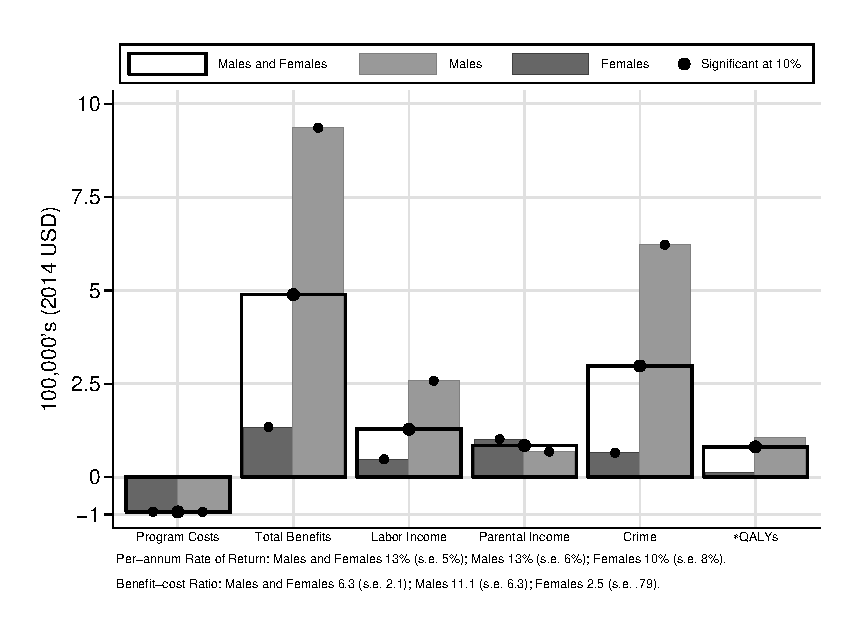
\includegraphics[width=.75\columnwidth]{output/abccare_npvssumm.eps}
\end{center}
\end{figure}
\end{frame}

\vspace{-16mm}
{\flushleft \small Note: This figure displays the life-cycle net present values per program participant of the main components of the cost/benefit analysis of ABC/CARE from birth to predicted death, discounted to birth at a rate of 3\%. By ``net" we mean that each component represents the total value for the treatment group minus the total value for the control group. Program costs: the total cost of ABC/CARE, including the welfare cost of taxes to finance it. Total net benefits: for \textit{all} of the components we consider. Labor income: total individual labor income from ages 20 to the retirement of program participants (assumed to be at age 67). Parental income: total parental labor income of the parents of the participants from when the participants were ages 1.5 to 21. Crime: the total cost of crime (judicial and victimization costs). To simplify the display, the following components are not shown in the figure: (i) cost of alternative preschool paid by the control group children parents; (ii) the social welfare costs of transfer income from the government; (iii) disability benefits and social security claims; (iv) costs of increased individual and maternal education (including special education and grade retention); (v) total medical public and private costs. Inference is based on non-parametric, one-sided $p$-values from the empirical bootstrap distribution. We indicate point estimates significant at the $10\%$ level.\\
*QALYs refers to the quality-adjusted life years. Any gain corresponds to better health conditions until predicted death, with $\$150,000$ (2014 USD) as base value for a year of life.\\}

\clearpage

%% -------------------------------------------------------------------------
\begin{frame}

\begin{table}[H]
\caption{Summary of Sensitivity Analyses for Cost/Benefit Analysis of the Program, Treatment vs. Next Best}\label{table:summsend}
\begin{center}
\mode<presentation>{\begin{tiny}}
\mode<article>{\begin{Large}}
\resizebox{\textwidth}{!}{
\begin{tabular}{lccc|ccc|ccc|ccc|ccc} \toprule
\underline{Component Set to Zero:}  & \multicolumn{3}{c}{None} & \multicolumn{3}{c}{Labor Income} &  \multicolumn{3}{c}{Parental Labor Income} &  \multicolumn{3}{c}{Crime} &  \multicolumn{3}{c}{*QALYs} \\ \\
\underline{Sample:} \\
Pooled & \checkmark &  &  & \checkmark &  &  & \checkmark &  &   & \checkmark &  &   & \checkmark &  &  \\
Male & & \checkmark &  & & \checkmark & & & \checkmark &  & & \checkmark &  & & \checkmark &  \\
Female & &  & \checkmark & &  & \checkmark & &  & \checkmark & &  & \checkmark & &  & \checkmark  \\  \\ \midrule

IRR & \textbf{0.14} & \textbf{0.15} & \textbf{0.10} & 	\textbf{0.13} &  \textbf{0.13} & 0.09 &		 \textbf{0.09} & \textbf{0.11} & 0.04  & 	\textbf{0.08}  & \textbf{0.09} & 0.10  & 		\textbf{0.13} & \textbf{0.14} & 0.09 \\
       & (0.03) & (0.04) & (0.06) &		 	(0.04) &  (0.05) & (0.06) &  			(0.03) &  (0.03) &  (0.02) & 			(0.04) & 	(0.05) & (0.06)   & 			(0.05) & (0.06) & (0.06) \\ \\

B/C Ratio & \textbf{7.33} & \textbf{10.19} & \textbf{2.61} & 	\textbf{6.03} & \textbf{7.75}  & \textbf{2.21} & \textbf{6.17} & \textbf{9.10} &  1.12 &  	\textbf{3.06} & 4.08 & \textbf{2.34}  & 		\textbf{6.48} & \textbf{9.14} & \textbf{2.20} \\
                 & (1.84) & (2.93) & (0.73) & 				(1.77) & (2.23) & (0.66) & 			(1.87) &  (2.92) &  (0.65) & 			(1.01) & (2.18) & (0.62)   & 	(1.79) & (2.73) & (0.69)  \\ \bottomrule
\end{tabular}
}
\mode<article>{\end{Large}}
\mode<presentation>{\end{tiny}}
\end{center}
\end{table}

{\flushleft \tiny Note: This table presents estimates of the internal rate of return (IRR) and the benefit-cost ratio (B/C Ratio) of ABC/CARE in scenarios where we set the net-present value of the estimated gain generated by the program of different components. ``None'' refers to the baseline estimation, where we do not set any of the components to zero. By ``net" we mean that each component represents the total value for the treatment group minus the total value for the control group. For details on the construction of each component, see Figure~\ref{figure:main}. Inference is based on non-parametric, one-sided $p$-values from the empirical bootstrap distribution. For the B/C ratio we use a discount rate of $3\%$. We test the null hypotheses $\text{IRR} = 3\%$ and $\text{B/C} = 1$---we elect $3\%$ because that is the discount rate we use. We indicate point estimates significant at the $10\%$ level. \\
*QALYs refers to the quality-adjusted life years. Any gain corresponds to better health conditions until predicted death, with $\$150,000$ (2014 USD) as base value for a year of life.\\}

\end{frame}

%% ---------------------------------------------------------------------------
\begin{frame}

\hypertarget{ret:scrambledeggs}{}
\begin{center}
\hyperlink{scrambledeggs}{\underline{Link to Program Details}}
\end{center}

\end{frame}

%% ---------------------------------------------------------------------------
\begin{frame}

\begin{block}{}
\begin{center}
\textbf{Program Analyzed}
\end{center}
\end{block}

\end{frame}

%% ---------------------------------------------------------------------------
\begin{frame}

\begin{itemize}
\item ABC/CARE Experiments
    \begin{enumerate}[(a)]
    \item Two very similar programs launched in the early 1970s that have long-term follow-ups through age 34
    \item Starts early (age 8 weeks)/intensive (8 hours a day) through age 5
    \item A second stage through age 8 that gave home visits but that had little effect
    \item Focus on the 8 weeks--age 5 segment
    \end{enumerate}
\end{itemize}

\hypertarget{ret:pancakeswaffles}{}
\begin{center}
\hyperlink{pancakeswaffles}{\underline{Link to ABC/CARE Tables}}
\end{center}

\end{frame}


%% ---------------------------------------------------------------------------

\begin{table}[H]
\caption{ABC and CARE, Program Comparison} \label{tab:programcomparison}
\begin{center}
\mode<presentation>{\begin{tiny}}
\mode<article>{\begin{normalsize}}
\begin{tabular}{L{4cm} L{2cm} L{2cm} C{1.5cm}} \toprule
& \multicolumn{1}{c}{ABC}& \multicolumn{1}{c}{CARE} & \multicolumn{1}{c}{ABC = CARE ?} \\ \midrule
\textbf{Program Overview} &&\\
\hspace{.2cm} Years Implemented &1972--1982&1978--1985\\
\hspace{.2cm} First-phase & Birth to 5 years old & Birth to 5 years old &\checkmark \\
\hspace{.2cm} Treatment & & & \\
\hspace{.2cm} Second-phase & 5 to 8 years old & 5 to 8 years old &\checkmark \\
\hspace{.2cm} Treatment & & & \\
\hspace{.2cm} Initially Recruited Sample &121&67\\
\hspace{.2cm} \# of Cohorts &4&2\\
\midrule
\textbf{Eligibility} & Socio-economic disadvantage according to a multi-factor index & Socio-economic disadvantage according to a multi-factor index & \checkmark\\
 \midrule
\textbf{Control} &&\\
\hspace{.2cm} N & 56 & 23\\
\hspace{.2cm} Compensation & Diapers from birth to age 3, unlimited formula from birth to 15 months & Diapers from birth to age 3, unlimited formula from birth to 15 months & \checkmark \\
\hspace{.2cm} Control   & \treatsubsabc & \treatsubscarec \\
\hspace{.2cm} Substitution & & \\
\bottomrule
\end{tabular}
\mode<article>{\end{normalsize}}
\mode<presentation>{\end{tiny}}
\end{center}
{\tiny \flushleft Note: This table compares the main elements of ABC and CARE, summarized in this section. A \checkmark indicates that ABC and CARE had the same feature. A blank space indicates that the indicated component was not part of the program.\\}
\end{table}

\begin{table}[H]\addtocounter{table}{-1}
\caption{ABC and CARE, Program Comparison} \label{tab:programcomparison}
\begin{center}
\mode<presentation>{\begin{tiny}}
\mode<article>{\begin{normalsize}}
\begin{tabular}{L{3cm} L{2.5cm} L{3cm} C{1cm}} \toprule
& \multicolumn{1}{c}{ABC}& \multicolumn{1}{c}{CARE} & \multicolumn{1}{c}{ABC = CARE ?} \\ \midrule
\textbf{Treatment} & Center-based childcare & Center-based childcare and family education\\
\hspace{.2cm} \textbf{Center-based} \\
\hspace{.2cm} \textbf{Childcare} \\
\hspace{.2cm} N & 58  & 17 \\
\hspace{.2cm} Intensity &6.5--9.75 hours a day for 50 weeks per year& 6.5--9.75 hours a day for 50 weeks per year & \checkmark\\
\hspace{.2cm} Components & Stimulation, medical care, nutrition, social services & Stimulation, medical care, nutrition, social services & \checkmark\\
\hspace{.2cm} Staff-to-child Ratio &1:3 during ages 0--1 &1:3 during ages 0--1 & \checkmark\\
&1:4--5 during age 1--4 &1:4--5 during age 1--4 & \checkmark\\
&1:5--6 during ages 4--5 & 1:5--6 during ages 4--5 & \checkmark\\
\hspace{.2cm} Staff Qualifications & Range of degrees beyond high school; experience in early childcare & Range of degrees beyond high school; experience in early childcare & \checkmark\\ \\
\bottomrule
\end{tabular}
\mode<article>{\end{normalsize}}
\mode<presentation>{\end{tiny}}
\end{center}
{\tiny \flushleft Note: This table compares the main elements of ABC and CARE, summarized in this section. A \checkmark indicates that ABC and CARE had the same feature. A blank space indicates that the indicated component was not part of the program.\\}
\end{table}

\begin{table}[H]\addtocounter{table}{-1}
\caption{ABC and CARE, Program Comparison} \label{tab:programcomparison}
\begin{center}
\mode<presentation>{\begin{tiny}}
\mode<article>{\begin{normalsize}}
\begin{tabular}{L{3cm} L{2.5cm} L{3cm} C{1cm}} \toprule
& \multicolumn{1}{c}{ABC}& \multicolumn{1}{c}{CARE} & \multicolumn{1}{c}{ABC = CARE ?} \\ \midrule
\textbf{Treatment} & Center-based childcare & Center-based childcare and family education\\
\hspace{.2cm} \textbf{Home Visitation}  & & \\
\hspace{.2cm} N & (not part of the program) &27\\
\hspace{.2cm} Intensity && Home visits lasting 1 hour. 2--3 times per month during ages 0--3. 1--2 times per month during ages 4--5\\
\hspace{.2cm} Curriculum & & Social and mental stimulation; parent-child interaction\\
\hspace{.2cm} Staff-to-child Ratio &&1:1\\
\hspace{.2cm} Staff Qualifications &&Home visitor training\\
\bottomrule
\end{tabular}
\mode<article>{\end{normalsize}}
\mode<presentation>{\end{tiny}}
\end{center}
{\tiny \flushleft Note: This table compares the main elements of ABC and CARE, summarized in this section. A \checkmark indicates that ABC and CARE had the same feature. A blank space indicates that the indicated component was not part of the program.\\}
\end{table}

\begin{table}[H]\addtocounter{table}{-1}
\caption{ABC and CARE, Program Comparison} \label{tab:programcomparison}
\begin{center}
\mode<presentation>{\begin{tiny}}
\mode<article>{\begin{normalsize}}
\begin{tabular}{L{4cm} L{2cm} L{2cm} C{1.5cm}} \toprule
& \multicolumn{1}{c}{ABC}& \multicolumn{1}{c}{CARE} & \multicolumn{1}{c}{ABC = CARE ?} \\
\midrule
\textbf{School-age Treatment} \\
\hspace{.2cm} Intensity & Every other week& Every other week & \checkmark\\
\hspace{.2cm} Components & Parent-teacher meetings& Parent-teacher meetings & \checkmark\\
\hspace{.2cm} Curriculum & Reading and math &  Reading and math & \checkmark\\
\hspace{.2cm} Staff Qualifications & Range of degrees beyond high school; experience in early childcare & Range of degrees beyond high school; experience in early childcare & \checkmark\\
\bottomrule
\end{tabular}
\mode<article>{\end{normalsize}}
\mode<presentation>{\end{tiny}}
\end{center}
{\tiny \flushleft Note: This table compares the main elements of ABC and CARE, summarized in this section. A \checkmark indicates that ABC and CARE had the same feature. A blank space indicates that the indicated component was not part of the program.\\}
\end{table}

%% ---------------------------------------------------------------------------
\begin{frame}

\begin{center}
\textbf{Goals of the Program}
\end{center}

\begin{itemize}
\item Goals: to remediate lifetime disadvantage by fostering the early-life skills of at-risk populations.
\item Focused primarily on African-American children.
    \begin{enumerate}[(i)]
    \item Supported language, motor, and cognitive development;
    \item Sought to minimize high-risk behaviors;
    \item Develop socio-emotional competencies considered crucial for school success including task-orientation, competence in communication, independence, and pro-social behavior.
    \end{enumerate}
\end{itemize}

\end{frame}

%% ---------------------------------------------------------------------------
\begin{frame}

\begin{itemize}
\item Full-day curriculum: emphasized active learning experiences, dramatic play, pre-academic skills (simple concepts of order, ranking, organization), and language skills.
\item For ages 3 through 5, as the cohorts approached public school entry, classroom experiences were increasingly structured towards the development of academic skills and ``socio-linguistic and communicative competence.''
\item Access to health screenings (but not costs of medication and costs of medical procedures)
\end{itemize}

\end{frame}

%% ---------------------------------------------------------------------------
\begin{frame}

\begin{center}
\textbf{Personalized Preschool}
\end{center}
\begin{itemize}
\item Highly personalized learning experiences for treated subjects in ABC/CARE.
\item Infant caregivers recorded child observations on progress charts and collaborated with curriculum developers and academic researchers to rotate learning activities every 2 to 3 weeks for each treated subject. (``Scaffolding'')
\end{itemize}

\end{frame}

%% ---------------------------------------------------------------------------
\begin{frame}

\begin{center}
\textbf{Childcare Friendly}
\end{center}
\begin{itemize}
\item For both ABC and CARE, centers were open to families from 7:45 a.m. to 5:30 p.m., 5 days per week, 50 weeks per year.
\item Subjects offered free transportation to and from the center.
\end{itemize}

\end{frame}

%%----------------------------------------------------------------------------
\begin{frame}

\begin{itemize}
\item Childcare
    \begin{itemize}
    \item Subsidized childcare supports other choices for mothers
        \begin{enumerate}[(i)]
        \item Promotes wage growth of women through work experience
        \item Educational attainment
        \end{enumerate}
    \end{itemize}
\item Avoids intergenerational costs of low-quality childcare on next generation child quality
\end{itemize}

\end{frame}

%% ---------------------------------------------------------------------------

\begin{itemize}
\item A driver and second adult staffed each vehicle (one van and two station wagons) equipped with child safety seats.
\item Data provided by Frank Porter Graham Center (FPGC) indicate that approximately 65\% of treated ABC families utilized the free transportation.
\item At FPGC, ABC and CARE treatment-group subjects received breakfast, lunch, and a snack planned by a nutritionist.
\end{itemize}

%% ---------------------------------------------------------------------------

\begin{itemize}
\item Varied educational backgrounds ranging from high school graduation to master's degrees.
\item Average professional working experience with young children: 7 years.
\item Child-caregiver ratios varied by age:
    \begin{itemize}
    \item 3:1 for infants up to 13 to 15 months of age
    \item 4:1 for toddlers up to 36 months
    \item 5:1 or 6:1 for children aged 3 to 5 years, depending on cohort size
    \end{itemize}
\end{itemize}

%% ---------------------------------------------------------------------------
\begin{frame}

\begin{center}
\textbf{Program Relevant Today}
\end{center}

\mode<presentation>{\begin{footnotesize}}
\begin{itemize}
\item Evidence from these programs is relevant for current policy discussions.
\item Their main features are found in a variety of programs in place around the world.
\mode<presentation>{\begin{footnotesize}}
\item Many successor programs use ABC/CARE as prototype
        \begin{itemize}\mode<presentation>{\begin{scriptsize}}
        \item Infant Health and Development Program (IHDP)---eight different cities around the U.S. \citep{Spiker-etal_1997_Helping};
        \item Early Head Start and Head Start in the U.S. \citep{Schneider_McDonald-eds_2007_Scale-Up_Vol-1};
        \item John's Hopkins Cerebral Palsy Study in the U.S. \citep{Sparling_2010_Highlights};
        \item CLIO study in the U.S. \citep{Sparling_2010_Highlights};
        \item Massachusetts Family Child Care Study \citep{Collins_etal_2010_Massachusetts-Study};
        \item Healthy Child Manitoba Evaluation \citep{Healthy_Child_Manitoba_2015_Starting-Early};
        \item Abecedarian Approach within an Innovative Implementation Framework \citep{Jensen_Nielsen_2016_ABC-Programme-Pilot};
        \item Building a Bridge into Preschool in Remote Northern Territory Communities in Australia \citep{UMonash_Dataset_2015_URL}.
        \item Educare programs are based on ABC/CARE \citep{Educare_2014_Research_Agenda,Yazejian_Bryant_2012_Educare}.\mode<presentation>{\end{scriptsize}}
        \end{itemize}
    \mode<presentation>{\end{footnotesize}}
\end{itemize}
\mode<presentation>{\end{footnotesize}}

\end{frame}

%% ---------------------------------------------------------------------------

\begin{itemize}
\item CLIO is the specific acronym for an ABC-based intervention to launched in the US. It stands for Classroom Literacy Interventions and Outcomes Study
\end{itemize}

%% ---------------------------------------------------------------------------
\begin{frame}

\begin{itemize}
\item Many children eligible for ABC/CARE in U.S.
\item 19\% of all African-American children in the U.S. today, 43\% at its inception
\item Corresponding figures for total population are 6\% and 15\%
\end{itemize}

\end{frame}

%% ---------------------------------------------------------------------------

\begin{itemize}
\item All four ABC cohorts and two CARE cohorts participated in curriculum developers Sparling and Lewis' ``LearningGames for the First Three Years.''
\item The ``LearningGames'' were implemented daily by infant and toddler caregivers in 1:1 child-adult interactions.
\item Each ``LearningGames'' activity stated a developmentally appropriate objective, the necessary materials, directions for teacher behavior, and expected child outcome.
\item The activities were designed for use both indoors and outdoors, while dressing, eating, bathing, or during play.
\item Benefit/cost ratios and rates of return are economically interpretable and policy-relevant summaries of the full impact of the program.
    \begin{itemize}
    \item Disaggregate into interpretable components by category.
    \item Improve on previous estimates by \citet{Barnett_Masse_2007_EER} who measure benefits only through age 21 (we go through 34), ignore welfare costs of taxes and do not report standard errors.
    \item We derive new estimates of program costs using recently available data (our estimates are higher).
    \end{itemize}
\item We currently have data only in the age range 30-34
\item Life-cycle CBA and rate of return analyses require projecting future benefits and costs over the lifetime
    \begin{enumerate}[(a)]
    \item Merge data from multiple panel data sources on earnings, health costs, crime, childcare savings, quality of life
    \item Account for sampling uncertainty
    \item Sensitivity analysis for cases where there is some uncertainty about numbers but no quantifiable components
    \end{enumerate}
\item We extend the analysis of \cite{Heckman_Moon_etal_2010_QE}
\end{itemize}

%% ---------------------------------------------------------------------------

\hypertarget{ret:protein}{}
\begin{center}
\hyperlink{protein}{\underline{Link to Data Availability for ABC and CARE}}
\end{center}

%% ---------------------------------------------------------------------------
\begin{frame}

\hypertarget{ret:potatochips}{}
\begin{center}
\hyperlink{potatochips}{\underline{Link to Tables of Full Experimental Data}}
\end{center}

\end{frame}

%% ---------------------------------------------------------------------------
\begin{frame}

\begin{center}
\textbf{Virtually all people offered treatment accepted it.}
\end{center}

\begin{itemize}
\item Non-compliance not an issue for treatment arm
\end{itemize}

\end{frame}

%% ---------------------------------------------------------------------------
\begin{frame}

\begin{center}
ABC Initial Sample: 121 Children \\(Randomized to Treatment or Control)
\end{center}

\begin{tabular}{lcc}
\toprule
\textbf{At Age 0:}  & $\star$58 treatment & $\star$56 control \\
\multicolumn{3}{c}{(7 dropouts after randomization)} \\ \\
\textbf{At School Age:}  & $\star$53 treatment & $\star$54 control \\
\multicolumn{3}{p{\textwidth}}{--net of: not followed-up (unknown reasons; moved to another city; death; developmentally delayed; replacements)} \\ \\
\textbf{At Age 21:}  & $\star$48 treatment & $\star$51 control \\
\textbf{At Age 30:}  & $\star$49 treatment & $\star$52 control \\
\bottomrule
\end{tabular}
\end{frame}

%% ---------------------------------------------------------------------------
\begin{frame}

\begin{center}
CARE Initial Sample: 67 Children \\(Randomized to Treatment or Control)
\end{center}

\begin{itemize}
\item 17 center-based care and family visits treatment group
\item 27 family visits treatment group
\item 23 control
\end{itemize}

\begin{center}
Throughout Followup:
\end{center}

\begin{itemize}
\item 5 cases: dead and not followed up in treatment group
\item 4 cases: dead and not followed up in control group
\end{itemize}

\end{frame}

%% ---------------------------------------------------------------------------
\begin{frame}

\begin{center}
\textbf{Framework and Notation}
\end{center}

\end{frame}

%% ---------------------------------------------------------------------------
\begin{frame}

\begin{equation*}
\underbrace{[0,...,\bar{a}\,]}_{\text{Treatment Period}} \;\; \underbrace{(\bar{a},...,a^{\ast}]}_{\text{Follow-up}} \;\; \underbrace{(a^{\ast},...,A]}_{\text{Remainder of Life Cycle}}
\end{equation*}

\end{frame}

%% ---------------------------------------------------------------------------

\begin{itemize}
\item Life cycles: $A+1$ discrete periods.
\item The treatment phase: first $\bar{a}$ periods of life $\left[0,\dots,\bar{a}\right]$.
\item Data through age $a^{*} > \bar{a}$.
\item Lack data on the remainder of life $[a^* + 1,\dots,A]$.
\item Needed for cost/benefit analysis.
\end{itemize}

%% ---------------------------------------------------------------------------
\begin{frame}

\begin{itemize}
\item Individuals eligible to participate in the program if baseline background variables $\bm{B}\in\mathcal{B}_0$.
\item $\mathcal{B}_0$: set of scores on the high risk index (HRI).
\end{itemize}

\end{frame}

%% ---------------------------------------------------------------------------
\begin{frame}

\hypertarget{ret:chocohocochip}{}
\begin{center}
\hyperlink{chocohocochip}{\underline{Link to Appendix:}}\\
Determinants of High Risk Index
\end{center}

\end{frame}

%% ---------------------------------------------------------------------------
\begin{frame}

\begin{itemize}
\item $W=1$: parents wish to participate in the program.
\item $R \in \{0,1\}$.
\item $R=1$ indicates that a child is randomized to be able to participate in the program.
\item $D$: participates in the program $(D \in \{ 0,1 \})$.
\item $D=RW$
\end{itemize}

\end{frame}

%% ---------------------------------------------------------------------------
\begin{frame}

\begin{itemize}
\item All eligible persons ($\bm{B}\in\mathcal{B}_0$) given the option to participate $(R=1)$ choose to participate in the program $(D=1)$.
\item Full compliance with the randomization: $R=1 \Rightarrow D=1$.
\item \emph{Ex ante} parents perceive that ABC/CARE was superior to other childcare alternatives.
\item \emph{Can safely interpret the treatment effects generated by the experiment as average treatment effects for the population for which $\bm{B}\in\mathcal{B}_0$ and not just treatment effects for the treated (\textbf{TOT}).}
\end{itemize}

\end{frame}

%% ---------------------------------------------------------------------------
\begin{frame}

\begin{itemize}
\item $\bm{Y}^1_a$: outcome vector for the treated.
\item $\bm{Y}^0_a$: outcome vector for those denied treatment in the program.
\end{itemize}

\end{frame}

%% ---------------------------------------------------------------------------
\begin{frame}

\begin{center}
\textbf{Exposure to Treatment}
\end{center}

\end{frame}

%% ---------------------------------------------------------------------------
\begin{frame}

\begin{itemize}
\item Life-cycle treatment effects for the controls and treatment group members might depend on the exposures to treatment or to the various alternatives at each age.
\item Few dropouts from the program (little variation in treatment exposure).
\item Pattern for controls: most start in home care at the earliest ages and move to alternative preschools as the child ages.
\item Once enrolled in an alternative preschool, they stay there through age 5.
\end{itemize}

\end{frame}

%% ---------------------------------------------------------------------------

\begin{figure}[H]
\caption{Control Substitution Characteristics, ABC/CARE Control Group}\label{fig:control-sub} \label{fig:salmonella}
\begin{center}
(a) Enrollment by Age \\
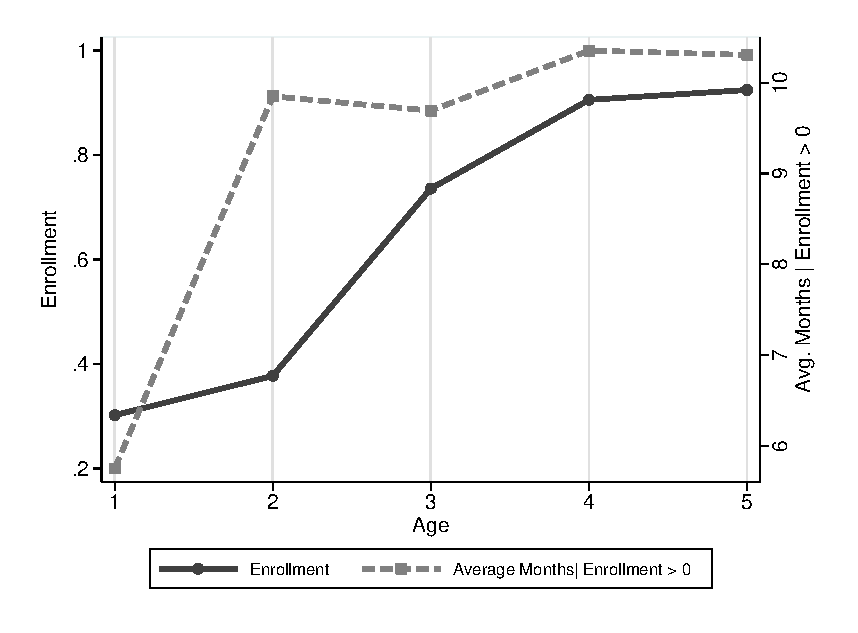
\includegraphics[width=.7\textwidth]{output/abccare_Valtenrollment.eps}
\end{center}
\end{figure}

\begin{figure}[H]
\addtocounter{figure}{-1}
\caption{Control Substitution Characteristics, ABC/CARE Control Group}\label{fig:control-sub} \label{fig:treatsubcare_2}
\begin{center}
(b) Enrollment Dynamics \\
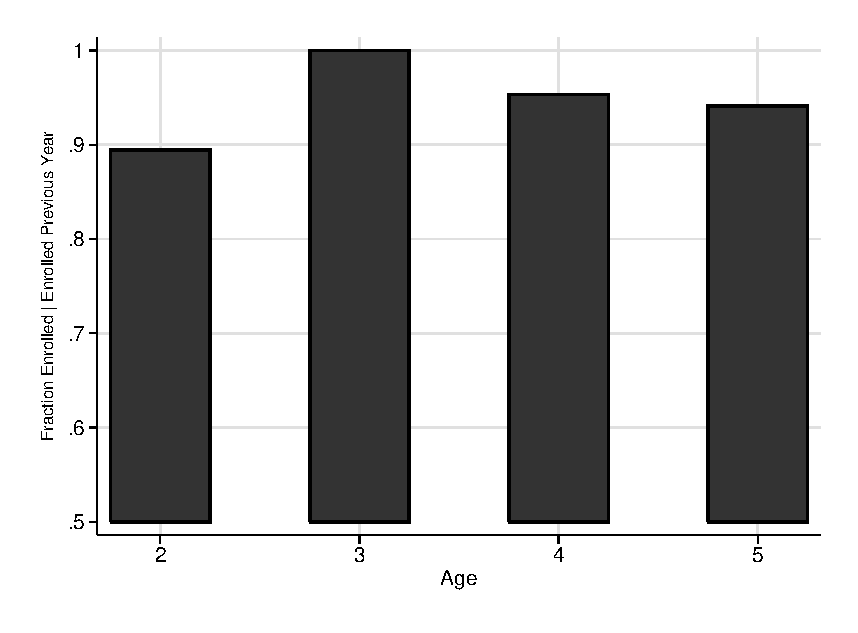
\includegraphics[width=.7\textwidth]{output/abccare_Vprobs.eps}
\end{center}
\end{figure}

%% ---------------------------------------------------------------------------
\begin{frame}

\begin{itemize}
\item  \textbf{Control-group substitution} or \textbf{substitution bias} (control group takes treatment)
\end{itemize}
\vspace{-2mm}
\begin{figure}[H]
\addtocounter{figure}{-1}
\caption{Months in Alternative Preschools (Control Group)}
\begin{center}
Enrollment \\
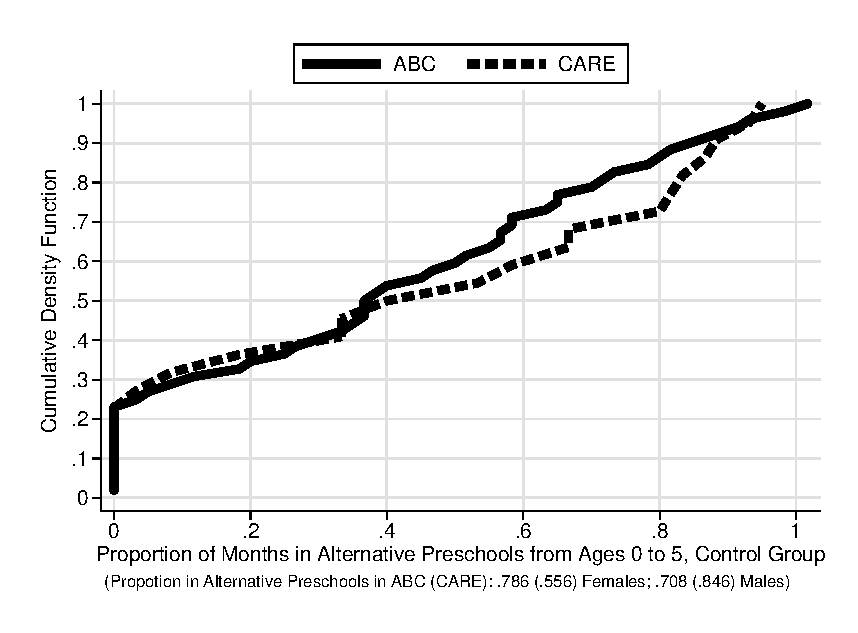
\includegraphics[width=0.55\textwidth]{output/abccare_controlcontamination.eps}
\end{center}
\end{figure}

\end{frame}

%% ---------------------------------------------------------------------------
\begin{frame}

\begin{figure}[H]
\addtocounter{figure}{-1}
\caption{Enrollment Transitions (Control Group)}\label{fig:control-sub} \label{fig:treatsubcare}
\begin{center}
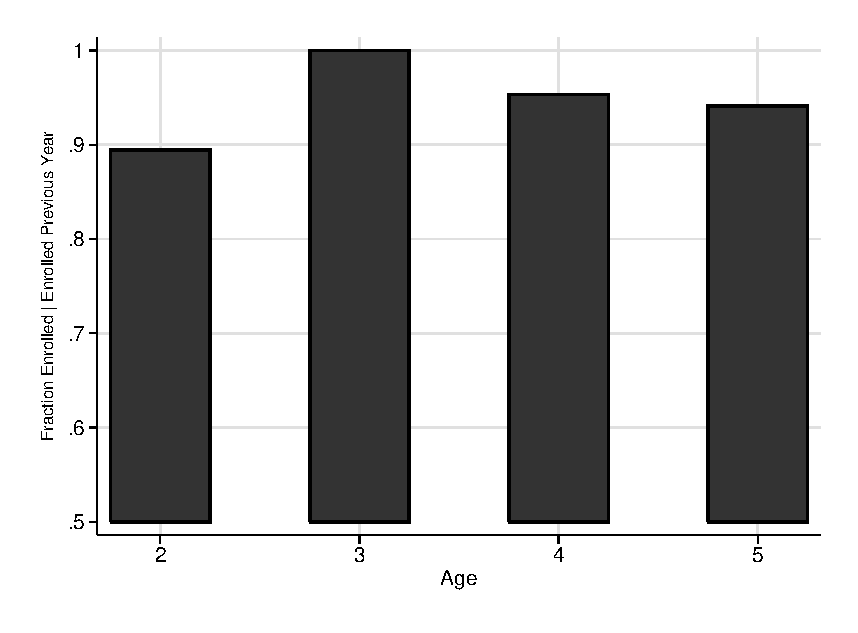
\includegraphics[width=.7\textwidth]{output/abccare_Vprobs.eps}
\end{center}
\end{figure}

\end{frame}

%% ---------------------------------------------------------------------------
\begin{frame}

\begin{center}
\textbf{Our Approach to Control Group Substitution}
\end{center}

\begin{itemize}
\item Sample sizes too small to make credible estimates of detailed control exposures.
\item Simplify the analysis by creating two categories of control status.
\item ``$\bm{H}$'' denotes that the child is in home care throughout the entire length of the program.
\item ``$\bm{C}$'' denotes that the child was in an alternative preschool anytime.
\end{itemize}

\end{frame}

%% ---------------------------------------------------------------------------
\begin{frame}

\begin{align*}
\bm{Y}_{a,H}^0 \quad &: \quad \textbf{ Subject received home care exclusively} \\
\bm{Y}_{a,C}^0 \quad &: \quad \textbf{ Subject received some alternative childcare}.
\end{align*}

\end{frame}

%% ---------------------------------------------------------------------------
\begin{frame}

\begin{itemize}
\item $V \in \{0,1\}$.
\item $V=1$: participation.
\item $V=0$: staying at home.
\item Control outcome $(\bm{Y}^0_a)$:
	\begin{equation}
	\bm{Y}^0_a : = \left( 1 - V \right) \bm{Y}^0_{a,H} + \left( V \right) \bm{Y}^0_{a,C}.
	\end{equation}
\end{itemize}

\end{frame}

%% ---------------------------------------------------------------------------
\begin{frame}

\begin{block}{}
\begin{center}
\textbf{Parameters of Interest}
\end{center}
\end{block}

\end{frame}

%% ---------------------------------------------------------------------------
\begin{frame}

\begin{itemize}
\item Random assignment does not guarantee that derived treatment effects answer policy-relevant questions.
\item Define and estimate three parameters that address different policy questions.
\end{itemize}

\end{frame}

%% ---------------------------------------------------------------------------
\begin{frame}

\begin{itemize}
\item Effect of program compared to the next best alternative as perceived by the parents:
	\begin{equation}\label{eq:effect}
	\bm{\Delta}_a := \mathbb{E} \left[ \bm{Y}^1_a -  \bm{Y}^0_a | W =1 \right] := \mathbb{E} \left[\bm{Y}^1_a - \bm{Y}^0_a | \bm{B} \in \mathcal{B}_0 \right]
	\end{equation}
\end{itemize}

\end{frame}

%% ---------------------------------------------------------------------------
\begin{frame}

\begin{center}
\textbf{Two Other Parameters}
\end{center}

\begin{itemize}
\item Effectiveness of the program with respect to a counterfactual world in which the child stays at home full time:
\end{itemize}
\mode<article>{\begin{large}}
\mode<presentation>{\begin{footnotesize}}
\begin{equation}\label{eq:influenza}
\bm{\Delta}_a \left(V = 0 \right) : =   \mathbb{E} \left[ \bm{Y}^1_a - \bm{Y}^0_a | V = 0, W = 1 \right] := \mathbb{E} \left[\bm{Y}^1_a - \bm{Y}^0_{a,H} | V = 0, 	\bm{B} \in \mathcal{B}_0 \right].
\end{equation}
\mode<presentation>{\end{footnotesize}}
\mode<article>{\end{large}}

\end{frame}

%% ---------------------------------------------------------------------------
\begin{frame}

\begin{itemize}
\item Effectiveness of a program relative to attendance in an alternative preschool for those who would choose an alternative:
\end{itemize}	
    \mode<article>{\begin{large}}
	\mode<presentation>{\begin{footnotesize}}
	\begin{equation}\label{eq:smallpox}
	\bm{\Delta}_a \left( V =1 \right) : =   \mathbb{E} \left[ \bm{Y}^1- \bm{Y}^0_a | V = 1, W = 1 \right] := \mathbb{E}  \left[\bm{Y}^1_a - \bm{Y}^0_{a,C} | V = 1, \bm{B} \in \mathcal{B}_0 \right].
	\end{equation}
	\mode<presentation>{\end{footnotesize}}
	\mode<article>{\end{large}}
\begin{itemize}
\item \textbf{Need non-experimental methods to analyze control group substitution}.
\end{itemize}

\end{frame}

\clearpage
%% ---------------------------------------------------------------------------

\begin{center}
\textbf{Alternative to Justify Centering at $\bm{1/2}$}
\end{center}

\begin{itemize}
\item Suppose that the treatment effect $\Delta_{j,a}$ has a null cumulative distribution associated to it. Denote this distribution by $\mathbb{F}_{j,a} \left( \cdot \right)$.
\item Assume that $\mathbb{F}_{j,a} \left( 0 \right) = 1/2$. Therefore, $\Pr \left( \Delta_{j,a} > 0 \right) = 1 - \Pr \left( \Delta_{j,a} \leq 0 \right) = 1 - \mathbb{F}_{j,a} \left( 0 \right) = 1/2$.
\item \emph{This states that under the null hypothesis a beneficial outcome is as likely as a non-beneficial outcome and enables us to show that $C_{l}/N_{l}$ is centered around $1/2$.} That is, \\$\mathbb{E} \left[ C_{l}/N_{l} \right] = 1/2$.
\end{itemize}

\begin{center}
\textbf{Alternative to Justify Centering at $\bm{1/2}$}
\end{center}

\begin{itemize}
\item To see this, note that $\mathbb{E}\left[ 1 ( \Delta_{j,a} >0)  \right] = \Pr \left( \Delta_{j,a} \leq 0 \right) \times 0  + \Pr \left( \Delta_{j,a} > 0 \right)  \times 1 = 1/2$ and therefore \\ $\mathbb{E} \left[ C_{l}  \right] = \mathbb{E} \left[ \sum^{N_l}_{j=1} 1 (\Delta_{j,a} >0) \right] = \sum^{N_l}_{j=1} \mathbb{E}\left[ 1 ( \Delta_{j,a} >0)  \right] = N_{l}/2$.
\item Thus, $\mathbb{E} \left[ C_{l}/N_{l} \right] = 1/2$.
\end{itemize}

%% ---------------------------------------------------------------------------
\begin{frame}

\begin{block}{}
\begin{center}
\textbf{Estimated Treatment Effects}
\end{center}
\end{block}

\end{frame}

%% ---------------------------------------------------------------------------
\begin{frame}
\begin{table}[H]
\caption{Treatment Effects on Selected Outcomes}\label{table:tescombined}
\begin{center}
\mode<presentation>{\begin{tiny}}
\mode<article>{\begin{Large}}
\resizebox{\textwidth}{!}{
\begin{tabular}{cccccccccccc}
\toprule
Category & Variable & Age & $\bar{Y}_c$ & (1) & (2) & (3) & (4) & (5) & (6)\\
\midrule
\multicolumn{9}{c}{\textbf{\emph{Females}}} \\ \\
           \mc{1}{l}{\tiny{Parental Income}} &   \mc{1}{l}{\tiny{Parental Labor Income}} & \mc{1}{c}{\tiny{3.5}} & 11,465 & \mc{1}{c}{\tiny{2,756}} & \mc{1}{c}{\tiny{2,986}} & \mc{1}{c}{\tiny{6,864}} & \mc{1}{c}{\tiny{8,584}} & \mc{1}{c}{\tiny{1,521}} & \mc{1}{c}{\tiny{3,773}} \\  

&   &  &  & \mc{1}{c}{\tiny{(0.189)}} & \mc{1}{c}{\tiny{(0.213)}} & \mc{1}{c}{\tiny{(0.122)}} & \mc{1}{c}{\tiny{\textbf{(0.045)}}} & \mc{1}{c}{\tiny{(0.332)}} & \mc{1}{c}{\tiny{(0.154)}} \\  

  &   & \mc{1}{c}{\tiny{12}} & 20,917 & \mc{1}{c}{\tiny{13,633}} & \mc{1}{c}{\tiny{19,592}} & \mc{1}{c}{\tiny{28,328}} & \mc{1}{c}{\tiny{26,489}} & \mc{1}{c}{\tiny{15,343}} & \mc{1}{c}{\tiny{18,678}} \\  

&   &  &  & \mc{1}{c}{\tiny{\textbf{(0.054)}}} & \mc{1}{c}{\tiny{\textbf{(0.027)}}} & \mc{1}{c}{\tiny{\textbf{(0.027)}}} & \mc{1}{c}{\tiny{\textbf{(0.009)}}} & \mc{1}{c}{\tiny{\textbf{(0.064)}}} & \mc{1}{c}{\tiny{\textbf{(0.019)}}} \\  

  &   & \mc{1}{c}{\tiny{15}} & 13,772 &\mc{1}{c}{\tiny{8,565}} & \mc{1}{c}{\tiny{7,159}} & \mc{1}{c}{\tiny{2,713}} & \mc{1}{c}{\tiny{8,441}} & \mc{1}{c}{\tiny{7,465}} & \mc{1}{c}{\tiny{10,487}} \\  

&  &   &  & \mc{1}{c}{\tiny{\textbf{(0.060)}}} & \mc{1}{c}{\tiny{(0.137)}} & \mc{1}{c}{\tiny{(0.480)}} & \mc{1}{c}{\tiny{(0.345)}} & \mc{1}{c}{\tiny{(0.134)}} & \mc{1}{c}{\tiny{\textbf{(0.064)}}} \\  

   &  & \mc{1}{c}{\tiny{21}} & 20,804 & \mc{1}{c}{\tiny{5,708}} & \mc{1}{c}{\tiny{8,670}} & \mc{1}{c}{\tiny{45,697}} & \mc{1}{c}{\tiny{25,142}} & \mc{1}{c}{\tiny{6,251}} & \mc{1}{c}{\tiny{3,943}} \\  

&  &   &  & \mc{1}{c}{\tiny{(0.136)}} & \mc{1}{c}{\tiny{(0.140)}} & \mc{1}{c}{\tiny{\textbf{(0.000)}}} & \mc{1}{c}{\tiny{\textbf{(0.000)}}} & \mc{1}{c}{\tiny{(0.224)}} & \mc{1}{c}{\tiny{(0.261)}} \\  

      \mc{1}{l}{\tiny{Education}} &  \mc{1}{l}{\tiny{Graduated High School}} & \mc{1}{c}{\tiny{30}} & 0.53 & \mc{1}{c}{\tiny{0.253}} & \mc{1}{c}{\tiny{0.131}} & \mc{1}{c}{\tiny{0.553}} & \mc{1}{c}{\tiny{0.595}} & \mc{1}{c}{\tiny{-0.026}} & \mc{1}{c}{\tiny{0.066}} \\  

& &    &  & \mc{1}{c}{\tiny{\textbf{(0.009)}}} & \mc{1}{c}{\tiny{(0.152)}} & \mc{1}{c}{\tiny{\textbf{(0.003)}}} & \mc{1}{c}{\tiny{\textbf{(0.000)}}} & \mc{1}{c}{\tiny{(0.413)}} & \mc{1}{c}{\tiny{(0.320)}} \\  

  &  \mc{1}{l}{\tiny{Years of Education}} & \mc{1}{c}{\tiny{30}} & 11.79 & \mc{1}{c}{\tiny{2.143}} & \mc{1}{c}{\tiny{1.843}} & \mc{1}{c}{\tiny{3.861}} & \mc{1}{c}{\tiny{3.923}} & \mc{1}{c}{\tiny{1.163}} & \mc{1}{c}{\tiny{1.409}} \\  

&  &   &  & \mc{1}{c}{\tiny{\textbf{(0.001)}}} & \mc{1}{c}{\tiny{\textbf{(0.002)}}} & \mc{1}{c}{\tiny{\textbf{(0.000)}}} & \mc{1}{c}{\tiny{\textbf{(0.000)}}} & \mc{1}{c}{\tiny{\textbf{(0.054)}}} & \mc{1}{c}{\tiny{\textbf{(0.017)}}} \\  

\bottomrule
\end{tabular}
}
\mode<article>{\end{Large}}
\mode<presentation>{\end{tiny}}
\end{center}
\end{table}
\vspace{-3.5mm}
{\flushleft \tiny Note: This table shows the treatment effects for categories outcomes that are important for our benefit/cost analysis. Systolic and diastolic blood pressure are measured in terms of mm Hg. Each column present estimates for the following parameters: \textbf{(1)} $\mathbb{E} \big[ \bm{Y}^1 - \bm{Y}^0 | W = 1]$; {\textbf{(2)} $\mathbb{E} \big[ \bm{Y}^1 - \bm{Y}^0 | \bm{B} \big]$}; {\textbf{(3)} $\mathbb{E} \big[ \bm{Y}^1 | \bm{B}, D=1 \big] - \mathbb{E} \big[ \bm{Y}^0 | \bm{B}, V=0, D=0 \big]$}; {\textbf{(4)} $\mathbb{E} \big[ \bm{Y}^1 - \bm{Y}^0 | \bm{B}, V=0 \big] $}; {\textbf{(5)} $\mathbb{E} \big[ \bm{Y}^1 | \bm{B}, D=1 \big] - \mathbb{E} \big[ \bm{Y}^0 | \bm{B}, V=1, D = 0 \big]$}; {\textbf{(6)} $\mathbb{E} \big[ \bm{Y}^1 - \bm{Y}^0 | \bm{B}, V=1 \big]$}. We account for the following background variables ($\bm{B}$): Apgar scores at minutes 1 and 5 of life and the high-risk index. Inference is based on non-parametric, one-sided $p$-values from the empirical bootstrap distribution. We highlight point estimates significant at the $10\%$ level. \\}

\end{frame}

%% ---------------------------------------------------------------------------
\begin{frame}

\begin{table}[H]\addtocounter{table}{-1}
\caption{Treatment Effects on Selected Outcomes, Cont'd}\label{table:tescombined}
\begin{center}
\mode<presentation>{\begin{tiny}}
\mode<article>{\begin{Large}}
\resizebox{\textwidth}{!}{
\begin{tabular}{ccccccccccc}
\toprule
Category & Variable & Age  & $\bar{Y}_c$  & (1) & (2) & (3) & (4) & (5) & (6)\\
\midrule
\multicolumn{9}{c}{\textbf{\emph{Females}}} \\ \\
 \mc{1}{l}{\tiny{Labor Income}} &  \mc{1}{l}{\tiny{Employed}} & \mc{1}{c}{\tiny{30}} & 0.71 & \mc{1}{c}{\tiny{0.131}} & \mc{1}{c}{\tiny{0.081}} & \mc{1}{c}{\tiny{0.381}} & \mc{1}{c}{\tiny{0.340}} & \mc{1}{c}{\tiny{-0.010}} & \mc{1}{c}{\tiny{0.070}} \\  

 &  &  &  & \mc{1}{c}{\tiny{\textbf{(0.096)}}} & \mc{1}{c}{\tiny{(0.206)}} & \mc{1}{c}{\tiny{\textbf{(0.039)}}} & \mc{1}{c}{\tiny{\textbf{(0.057)}}} & \mc{1}{c}{\tiny{(0.465)}} & \mc{1}{c}{\tiny{(0.264)}} \\  

  &  \mc{1}{l}{\tiny{Labor Income}} & \mc{1}{c}{\tiny{30}} & 23,267 & \mc{1}{c}{\tiny{2,548}} & \mc{1}{c}{\tiny{1,884}} & \mc{1}{c}{\tiny{15,094}} & \mc{1}{c}{\tiny{13,096}} & \mc{1}{c}{\tiny{-2,677}} & \mc{1}{c}{\tiny{-2,122}} \\  

&  &   &  & \mc{1}{c}{\tiny{(0.335)}} & \mc{1}{c}{\tiny{(0.382)}} & \mc{1}{c}{\tiny{\textbf{(0.056)}}} & \mc{1}{c}{\tiny{\textbf{(0.022)}}} & \mc{1}{c}{\tiny{(0.330)}} & \mc{1}{c}{\tiny{(0.363)}} \\  

     \mc{1}{l}{\tiny{Crime}} &   \mc{1}{l}{\tiny{Total Felony Arrests}} & \mc{1}{c}{\tiny{Mid-30s}} & 0.42 & \mc{1}{c}{\tiny{-0.328}} & \mc{1}{c}{\tiny{-0.351}} & \mc{1}{c}{\tiny{-0.944}} & \mc{1}{c}{\tiny{-0.965}} & \mc{1}{c}{\tiny{-0.059}} & \mc{1}{c}{\tiny{0.004}} \\  

& &    &  & \mc{1}{c}{\tiny{\textbf{(0.077)}}} & \mc{1}{c}{\tiny{\textbf{(0.087)}}} & \mc{1}{c}{\tiny{\textbf{(0.095)}}} & \mc{1}{c}{\tiny{\textbf{(0.095)}}} & \mc{1}{c}{\tiny{(0.287)}} & \mc{1}{c}{\tiny{(0.500)}} \\  

 &   \mc{1}{l}{\tiny{Total Misdemeanor Arrests}} & \mc{1}{c}{\tiny{Mid-30s}}& 1.16 & \mc{1}{c}{\tiny{-0.973}} & \mc{1}{c}{\tiny{-0.737}} & \mc{1}{c}{\tiny{-2.010}} & \mc{1}{c}{\tiny{-2.451}} & \mc{1}{c}{\tiny{-0.269}} & \mc{1}{c}{\tiny{-0.201}} \\  

&  &    &  & \mc{1}{c}{\tiny{\textbf{(0.057)}}} & \mc{1}{c}{\tiny{(0.134)}} & \mc{1}{c}{\tiny{(0.134)}} & \mc{1}{c}{\tiny{(0.120)}} & \mc{1}{c}{\tiny{(0.273)}} & \mc{1}{c}{\tiny{(0.289)}} \\  

     \mc{1}{l}{\tiny{Health}} &   \mc{1}{l}{\tiny{Self-reported drug user}} & \mc{1}{c}{\tiny{Mid-30s}} & 0.26 & \mc{1}{c}{\tiny{-0.033}} & \mc{1}{c}{\tiny{0.004}} & \mc{1}{c}{\tiny{-0.114}} & \mc{1}{c}{\tiny{-0.101}} & \mc{1}{c}{\tiny{0.020}} & \mc{1}{c}{\tiny{0.033}} \\  

&  &    &  & \mc{1}{c}{\tiny{(0.381)}} & \mc{1}{c}{\tiny{(0.478)}} & \mc{1}{c}{\tiny{(0.273)}} & \mc{1}{c}{\tiny{(0.323)}} & \mc{1}{c}{\tiny{(0.443)}} & \mc{1}{c}{\tiny{(0.406)}} \\  

  &  \mc{1}{l}{\tiny{Systolic Blood Pressure (mm Hg)}} & \mc{1}{c}{\tiny{Mid-30s}} & 133.96 & \mc{1}{c}{\tiny{-2.899}} & \mc{1}{c}{\tiny{-5.407}} & \mc{1}{c}{\tiny{-0.488}} & \mc{1}{c}{\tiny{-0.822}} & \mc{1}{c}{\tiny{-6.239}} & \mc{1}{c}{\tiny{-6.784}} \\  

&  &   &  & \mc{1}{c}{\tiny{(0.307)}} & \mc{1}{c}{\tiny{(0.241)}} & \mc{1}{c}{\tiny{(0.488)}} & \mc{1}{c}{\tiny{(0.457)}} & \mc{1}{c}{\tiny{(0.249)}} & \mc{1}{c}{\tiny{(0.170)}} \\  

  &  \mc{1}{l}{\tiny{Diastolic Blood Pressure (mm Hg)}} & \mc{1}{c}{\tiny{Mid-30s}} & 87.56 & \mc{1}{c}{\tiny{-0.002}} & \mc{1}{c}{\tiny{-0.179}} & \mc{1}{c}{\tiny{4.091}} & \mc{1}{c}{\tiny{4.122}} & \mc{1}{c}{\tiny{-1.347}} & \mc{1}{c}{\tiny{-2.160}} \\  

&  &   &  & \mc{1}{c}{\tiny{(0.483)}} & \mc{1}{c}{\tiny{(0.438)}} & \mc{1}{c}{\tiny{(0.245)}} & \mc{1}{c}{\tiny{(0.222)}} & \mc{1}{c}{\tiny{(0.392)}} & \mc{1}{c}{\tiny{(0.339)}} \\  

  &  \mc{1}{l}{\tiny{Hypertension}} & \mc{1}{c}{\tiny{Mid-30s}} & 0.41 & \mc{1}{c}{\tiny{0.172}} & \mc{1}{c}{\tiny{0.085}} & \mc{1}{c}{\tiny{0.077}} & \mc{1}{c}{\tiny{0.162}} & \mc{1}{c}{\tiny{0.102}} & \mc{1}{c}{\tiny{0.107}} \\  

&  &   &  & \mc{1}{c}{\tiny{(0.111)}} & \mc{1}{c}{\tiny{(0.293)}} & \mc{1}{c}{\tiny{(0.331)}} & \mc{1}{c}{\tiny{(0.245)}} & \mc{1}{c}{\tiny{(0.299)}} & \mc{1}{c}{\tiny{(0.255)}} \\  
\bottomrule
\end{tabular}
}
\mode<article>{\end{Large}}
\mode<presentation>{\end{tiny}}
\end{center}
\end{table}
\vspace{-3.5mm}
{\flushleft \tiny Note: This table shows the treatment effects for categories outcomes that are important for our benefit/cost analysis. Systolic and diastolic blood pressure are measured in terms of mm Hg. Each column present estimates for the following parameters: \textbf{(1)} $\mathbb{E} \big[ \bm{Y}^1 - \bm{Y}^0 | W = 1]$; {\textbf{(2)} $\mathbb{E} \big[ \bm{Y}^1 - \bm{Y}^0 | \bm{B} \big]$}; {\textbf{(3)} $\mathbb{E} \big[ \bm{Y}^1 | \bm{B}, D=1 \big] - \mathbb{E} \big[ \bm{Y}^0 | \bm{B}, V=0, D=0 \big]$}; {\textbf{(4)} $\mathbb{E} \big[ \bm{Y}^1 - \bm{Y}^0 | \bm{B}, V=0 \big] $}; {\textbf{(5)} $\mathbb{E} \big[ \bm{Y}^1 | \bm{B}, D=1 \big] - \mathbb{E} \big[ \bm{Y}^0 | \bm{B}, V=1, D = 0 \big]$}; {\textbf{(6)} $\mathbb{E} \big[ \bm{Y}^1 - \bm{Y}^0 | \bm{B}, V=1 \big]$}. We account for the following background variables ($\bm{B}$): Apgar scores at minutes 1 and 5 of life and the high-risk index. Inference is based on non-parametric, one-sided $p$-values from the empirical bootstrap distribution. We highlight point estimates significant at the $10\%$ level. \\}

\end{frame}

%% ---------------------------------------------------------------------------
\begin{frame}

\begin{table}[H]
\addtocounter{table}{-1}
\caption{Treatment Effects on Selected Outcomes, Cont'd}\label{table:tescombined}
\begin{center}
\mode<presentation>{\begin{tiny}}
\mode<article>{\begin{Large}}
\resizebox{\textwidth}{!}{
\begin{tabular}{cccccccccccc}
\toprule
Category & Variable & Age & $\bar{Y}_c$  & (1) & (2) & (3) & (4) & (5) & (6)\\
\midrule
\multicolumn{9}{c}{\textbf{\emph{Males}}} \\ \\
\mc{1}{l}{\tiny{Parental Income}} &   \mc{1}{l}{\tiny{Parental Labor Income}} & \mc{1}{c}{\tiny{3.5}} & 13,505 & \mc{1}{c}{\tiny{1,036}} & \mc{1}{c}{\tiny{494}} & \mc{1}{c}{\tiny{73.862}} & \mc{1}{c}{\tiny{1,462}} & \mc{1}{c}{\tiny{123}} & \mc{1}{c}{\tiny{690}} \\  

&  &   &  & \mc{1}{c}{\tiny{(0.374)}} & \mc{1}{c}{\tiny{(0.411)}} & \mc{1}{c}{\tiny{(0.474)}} & \mc{1}{c}{\tiny{(0.390)}} & \mc{1}{c}{\tiny{(0.479)}} & \mc{1}{c}{\tiny{(0.417)}} \\  

  &   & \mc{1}{c}{\tiny{12}} & 23,868 & \mc{1}{c}{\tiny{7,085}} & \mc{1}{c}{\tiny{9,625}} & \mc{1}{c}{\tiny{18,050}} & \mc{1}{c}{\tiny{12,639}} & \mc{1}{c}{\tiny{6,620}} & \mc{1}{c}{\tiny{5,383}} \\  

&  &   &  & \mc{1}{c}{\tiny{\textbf{(0.092)}}} & \mc{1}{c}{\tiny{\textbf{(0.020)}}} & \mc{1}{c}{\tiny{\textbf{(0.038)}}} & \mc{1}{c}{\tiny{\textbf{(0.074)}}} & \mc{1}{c}{\tiny{\textbf{(0.098)}}} & \mc{1}{c}{\tiny{(0.139)}} \\  

  &   & \mc{1}{c}{\tiny{15}} & 22,985& \mc{1}{c}{\tiny{8,488}} & \mc{1}{c}{\tiny{4,495}} & \mc{1}{c}{\tiny{5,540}} & \mc{1}{c}{\tiny{4,805}} & \mc{1}{c}{\tiny{2,885}} & \mc{1}{c}{\tiny{4,345}} \\  

&  &   &  & \mc{1}{c}{\tiny{\textbf{(0.071)}}} & \mc{1}{c}{\tiny{(0.221)}} & \mc{1}{c}{\tiny{(0.243)}} & \mc{1}{c}{\tiny{(0.264)}} & \mc{1}{c}{\tiny{(0.354)}} & \mc{1}{c}{\tiny{(0.296)}} \\  

  &   & \mc{1}{c}{\tiny{21}} & 21,585 &\mc{1}{c}{\tiny{12,732}} & \mc{1}{c}{\tiny{8,809}} & \mc{1}{c}{\tiny{122}} & \mc{1}{c}{\tiny{-933}} & \mc{1}{c}{\tiny{10,784}} & \mc{1}{c}{\tiny{10,283}} \\  

&  &   &  & \mc{1}{c}{\tiny{\textbf{(0.005)}}} & \mc{1}{c}{\tiny{\textbf{(0.098)}}} & \mc{1}{c}{\tiny{(0.448)}} & \mc{1}{c}{\tiny{(0.456)}} & \mc{1}{c}{\tiny{\textbf{(0.056)}}} & \mc{1}{c}{\tiny{\textbf{(0.041)}}} \\  

   \mc{1}{l}{\tiny{Education}} &   \mc{1}{l}{\tiny{Graduated High School}} & \mc{1}{c}{\tiny{30}} & 0.60 & \mc{1}{c}{\tiny{0.073}} & \mc{1}{c}{\tiny{0.044}} & \mc{1}{c}{\tiny{0.116}} & \mc{1}{c}{\tiny{0.083}} & \mc{1}{c}{\tiny{0.040}} & \mc{1}{c}{\tiny{0.063}} \\  

&  &   &  & \mc{1}{c}{\tiny{(0.262)}} & \mc{1}{c}{\tiny{(0.375)}} & \mc{1}{c}{\tiny{\textbf{(0.001)}}} & \mc{1}{c}{\tiny{(0.346)}} & \mc{1}{c}{\tiny{(0.407)}} & \mc{1}{c}{\tiny{(0.317)}} \\  

  &  \mc{1}{l}{\tiny{Graduated 4-year College}} & \mc{1}{c}{\tiny{30}} & 0.12 & \mc{1}{c}{\tiny{0.170}} & \mc{1}{c}{\tiny{0.138}} & \mc{1}{c}{\tiny{0.149}} & \mc{1}{c}{\tiny{0.099}} & \mc{1}{c}{\tiny{0.135}} & \mc{1}{c}{\tiny{0.143}} \\  

&  &   &  & \mc{1}{c}{\tiny{\textbf{(0.055)}}} & \mc{1}{c}{\tiny{(0.128)}} & \mc{1}{c}{\tiny{(0.216)}} & \mc{1}{c}{\tiny{(0.338)}} & \mc{1}{c}{\tiny{(0.154)}} & \mc{1}{c}{\tiny{(0.130)}} \\  

  &  \mc{1}{l}{\tiny{Years of Education}} & \mc{1}{c}{\tiny{30}} & 12.87 & \mc{1}{c}{\tiny{0.525}} & \mc{1}{c}{\tiny{0.541}} & \mc{1}{c}{\tiny{1.010}} & \mc{1}{c}{\tiny{0.777}} & \mc{1}{c}{\tiny{0.351}} & \mc{1}{c}{\tiny{0.344}} \\  

&  &   &  & \mc{1}{c}{\tiny{(0.151)}} & \mc{1}{c}{\tiny{(0.163)}} & \mc{1}{c}{\tiny{(0.998)}} & \mc{1}{c}{\tiny{(0.136)}} & \mc{1}{c}{\tiny{(0.280)}} & \mc{1}{c}{\tiny{(0.256)}} \\  
\bottomrule
    \end{tabular}
}
\mode<article>{\end{Large}}
\mode<presentation>{\end{tiny}}
\end{center}
\end{table}
\vspace{-3.5mm}
{\flushleft \tiny Note: This table shows the treatment effects for categories outcomes that are important for our benefit/cost analysis. Systolic and diastolic blood pressure are measured in terms of mm Hg. Each column present estimates for the following parameters: \textbf{(1)} $\mathbb{E} \big[ \bm{Y}^1 - \bm{Y}^0 | W = 1]$; {\textbf{(2)} $\mathbb{E} \big[ \bm{Y}^1 - \bm{Y}^0 | \bm{B} \big]$}; {\textbf{(3)} $\mathbb{E} \big[ \bm{Y}^1 | \bm{B}, D=1 \big] - \mathbb{E} \big[ \bm{Y}^0 | \bm{B}, V=0, D=0 \big]$}; {\textbf{(4)} $\mathbb{E} \big[ \bm{Y}^1 - \bm{Y}^0 | \bm{B}, V=0 \big] $}; {\textbf{(5)} $\mathbb{E} \big[ \bm{Y}^1 | \bm{B}, D=1 \big] - \mathbb{E} \big[ \bm{Y}^0 | \bm{B}, V=1, D = 0 \big]$}; {\textbf{(6)} $\mathbb{E} \big[ \bm{Y}^1 - \bm{Y}^0 | \bm{B}, V=1 \big]$}. We account for the following background variables ($\bm{B}$): Apgar scores at minutes 1 and 5 of life and the high-risk index. Inference is based on non-parametric, one-sided $p$-values from the empirical bootstrap distribution. We highlight point estimates significant at the $10\%$ level. \\}

\end{frame}


%% ---------------------------------------------------------------------------
\begin{frame}

\begin{table}[H]
\addtocounter{table}{-1}
\caption{Treatment Effects on Selected Outcomes, Cont'd}\label{table:tescombined}
\begin{center}
\mode<presentation>{\begin{tiny}}
\mode<article>{\begin{Large}}
\resizebox{\textwidth}{!}{
\begin{tabular}{ccccccccccc}
\toprule
Category & Variable & Age & $\bar{Y}_c$ & (1) & (2) & (3) & (4) & (5) & (6)\\
\midrule
\multicolumn{9}{c}{\textbf{\emph{Males}}} \\ \\
 \mc{1}{l}{\tiny{Labor Income}} &   \mc{1}{l}{\tiny{Employed}} & \mc{1}{c}{\tiny{30}} & 0.70 & \mc{1}{c}{\tiny{0.119}} & \mc{1}{c}{\tiny{0.196}} & \mc{1}{c}{\tiny{0.108}} & \mc{1}{c}{\tiny{0.040}} & \mc{1}{c}{\tiny{0.237}} & \mc{1}{c}{\tiny{0.261}} \\  

& &    &  & \mc{1}{c}{\tiny{(0.128)}} & \mc{1}{c}{\tiny{\textbf{(0.025)}}} & \mc{1}{c}{\tiny{\textbf{(0.001)}}} & \mc{1}{c}{\tiny{(0.383)}} & \mc{1}{c}{\tiny{\textbf{(0.025)}}} & \mc{1}{c}{\tiny{\textbf{(0.013)}}} \\  

  &  \mc{1}{l}{\tiny{Labor Income}} & \mc{1}{c}{\tiny{30}}& 30,079 & \mc{1}{c}{\tiny{19,810}} & \mc{1}{c}{\tiny{24,365}} & \mc{1}{c}{\tiny{25,220}} & \mc{1}{c}{\tiny{20,611}} & \mc{1}{c}{\tiny{23,072}} & \mc{1}{c}{\tiny{21,836}} \\  

&   &  &  & \mc{1}{c}{\tiny{\textbf{(0.091)}}} & \mc{1}{c}{\tiny{\textbf{(0.092)}}} & \mc{1}{c}{\tiny{(0.998)}} & \mc{1}{c}{\tiny{(0.122)}} & \mc{1}{c}{\tiny{(0.107)}} & \mc{1}{c}{\tiny{\textbf{(0.094)}}} \\  

  \mc{1}{l}{\tiny{Crime}} &    \mc{1}{l}{\tiny{Total Felony Arrests}} & \mc{1}{c}{\tiny{Mid-30s}} & 1.37 & \mc{1}{c}{\tiny{0.196}} & \mc{1}{c}{\tiny{0.685}} & \mc{1}{c}{\tiny{1.523}} & \mc{1}{c}{\tiny{1.340}} & \mc{1}{c}{\tiny{0.481}} & \mc{1}{c}{\tiny{0.188}} \\  

&   &  &  & \mc{1}{c}{\tiny{(0.368)}} & \mc{1}{c}{\tiny{(0.183)}} & \mc{1}{c}{\tiny{\textbf{(0.064)}}} & \mc{1}{c}{\tiny{\textbf{(0.026)}}} & \mc{1}{c}{\tiny{(0.284)}} & \mc{1}{c}{\tiny{(0.410)}} \\  

  &  \mc{1}{l}{\tiny{Total Misdemeanor Arrests}} & \mc{1}{c}{\tiny{Mid-30s}} & 1.30 & \mc{1}{c}{\tiny{-0.501}} & \mc{1}{c}{\tiny{-0.244}} & \mc{1}{c}{\tiny{-0.298}} & \mc{1}{c}{\tiny{-0.034}} & \mc{1}{c}{\tiny{-0.246}} & \mc{1}{c}{\tiny{-0.507}} \\  

&  &   &  & \mc{1}{c}{\tiny{(0.171)}} & \mc{1}{c}{\tiny{(0.289)}} & \mc{1}{c}{\tiny{(0.314)}} & \mc{1}{c}{\tiny{(0.422)}} & \mc{1}{c}{\tiny{(0.329)}} & \mc{1}{c}{\tiny{(0.168)}} \\  

   \mc{1}{l}{\tiny{Health}} &   \mc{1}{l}{\tiny{Self-reported drug user}} & \mc{1}{c}{\tiny{Mid-30s}} & 0.50 & \mc{1}{c}{\tiny{-0.333}} & \mc{1}{c}{\tiny{-0.438}} & \mc{1}{c}{\tiny{-0.673}} & \mc{1}{c}{\tiny{-0.557}} & \mc{1}{c}{\tiny{-0.326}} & \mc{1}{c}{\tiny{-0.330}} \\  

&   &  &  & \mc{1}{c}{\tiny{\textbf{(0.019)}}} & \mc{1}{c}{\tiny{\textbf{(0.002)}}} & \mc{1}{c}{\tiny{\textbf{(0.000)}}} & \mc{1}{c}{\tiny{\textbf{(0.000)}}} & \mc{1}{c}{\tiny{\textbf{(0.039)}}} & \mc{1}{c}{\tiny{\textbf{(0.023)}}} \\  

  &  \mc{1}{l}{\tiny{Systolic Blood Pressure (mm Hg)}} & \mc{1}{c}{\tiny{Mid-30s}} & 138.07 & \mc{1}{c}{\tiny{-9.791}} & \mc{1}{c}{\tiny{-13.275}} & \mc{1}{c}{\tiny{14.196}} & \mc{1}{c}{\tiny{14.976}} & \mc{1}{c}{\tiny{-24.166}} & \mc{1}{c}{\tiny{-18.559}} \\  

&  &   &  & \mc{1}{c}{\tiny{(0.113)}} & \mc{1}{c}{\tiny{\textbf{(0.049)}}} & \mc{1}{c}{\tiny{\textbf{(0.013)}}} & \mc{1}{c}{\tiny{\textbf{(0.000)}}} & \mc{1}{c}{\tiny{\textbf{(0.000)}}} & \mc{1}{c}{\tiny{\textbf{(0.011)}}} \\  

  &  \mc{1}{l}{\tiny{Diastolic Blood Pressure (mm Hg)}} & \mc{1}{c}{\tiny{Mid-30s}} & 89.21 & \mc{1}{c}{\tiny{-10.854}} & \mc{1}{c}{\tiny{-14.134}} & \mc{1}{c}{\tiny{-9.709}} & \mc{1}{c}{\tiny{-8.741}} & \mc{1}{c}{\tiny{-18.387}} & \mc{1}{c}{\tiny{-13.987}} \\  

&  &   &  & \mc{1}{c}{\tiny{\textbf{(0.032)}}} & \mc{1}{c}{\tiny{\textbf{(0.004)}}} & \mc{1}{c}{\tiny{\textbf{(0.049)}}} & \mc{1}{c}{\tiny{\textbf{(0.032)}}} & \mc{1}{c}{\tiny{\textbf{(0.000)}}} & \mc{1}{c}{\tiny{\textbf{(0.007)}}} \\  

  &  \mc{1}{l}{\tiny{Hypertension}} & \mc{1}{c}{\tiny{Mid-30s}}& 0.57 & \mc{1}{c}{\tiny{-0.291}} & \mc{1}{c}{\tiny{-0.377}} & \mc{1}{c}{\tiny{-0.120}} & \mc{1}{c}{\tiny{-0.074}} & \mc{1}{c}{\tiny{-0.492}} & \mc{1}{c}{\tiny{-0.434}} \\  

&   &  &  & \mc{1}{c}{\tiny{\textbf{(0.042)}}} & \mc{1}{c}{\tiny{\textbf{(0.009)}}} & \mc{1}{c}{\tiny{(0.302)}} & \mc{1}{c}{\tiny{(0.353)}} & \mc{1}{c}{\tiny{\textbf{(0.006)}}} & \mc{1}{c}{\tiny{\textbf{(0.006)}}} \\  
\bottomrule
    \end{tabular}
}
\mode<article>{\end{Large}}
\mode<presentation>{\end{tiny}}
\end{center}
\end{table}
\vspace{-3.5mm}
{\flushleft \tiny Note: This table shows the treatment effects for categories outcomes that are important for our benefit/cost analysis. Systolic and diastolic blood pressure are measured in terms of mm Hg. Each column present estimates for the following parameters: \textbf{(1)} $\mathbb{E} \big[ \bm{Y}^1 - \bm{Y}^0 | W = 1]$; {\textbf{(2)} $\mathbb{E} \big[ \bm{Y}^1 - \bm{Y}^0 | \bm{B} \big]$}; {\textbf{(3)} $\mathbb{E} \big[ \bm{Y}^1 | \bm{B}, D=1 \big] - \mathbb{E} \big[ \bm{Y}^0 | \bm{B}, V=0, D=0 \big]$}; {\textbf{(4)} $\mathbb{E} \big[ \bm{Y}^1 - \bm{Y}^0 | \bm{B}, V=0 \big] $}; {\textbf{(5)} $\mathbb{E} \big[ \bm{Y}^1 | \bm{B}, D=1 \big] - \mathbb{E} \big[ \bm{Y}^0 | \bm{B}, V=1, D = 0 \big]$}; {\textbf{(6)} $\mathbb{E} \big[ \bm{Y}^1 - \bm{Y}^0 | \bm{B}, V=1 \big]$}. We account for the following background variables ($\bm{B}$): Apgar scores at minutes 1 and 5 of life and the high-risk index. Inference is based on non-parametric, one-sided $p$-values from the empirical bootstrap distribution. We highlight point estimates significant at the $10\%$ level. \\}

\end{frame}

%% ---------------------------------------------------------------------------
\begin{frame}

\hypertarget{ret:frosting}{}
\begin{center}
\hyperlink{frosting}{\underline{Link to Appendix:}}\\
Treatment Effects Accounting Correcting the $p$-values Using Step-down (Romano-Wolf; Romano-Shaikh)
\end{center}

\end{frame}

\clearpage
%%-------------------------------------------------------------------------
\begin{frame}

\begin{block}{}
\begin{center}
\textbf{Predicting and Monetizing Life-cycle Costs and Benefits}
\end{center}
\end{block}

\end{frame}

%% ------------------------------------------------------------------------------------------------
\begin{frame}

\begin{itemize}
\item Predicting post-sample life cycle benefits.
\item Our approach starts from and extends the analysis of \citet{Heckman_Pinto_etal_2013_PerryFactor}.
\item \textbf{The effect of treatment on outcomes operates through its effects on inputs in a stable production function.}
\item Table~\ref{table:sources} presents the outcomes for which we conduct these analyses and the data sources used.
\end{itemize}

\end{frame}


\begin{frame}

\begin{center}
\textbf{Overview of Predictions}
\end{center}

\end{frame}

%% ------------------------------------------------------------------------------------------------
\begin{frame}

\begin{center}
\textbf{Using Auxiliary Data Sources to Predict\\ Out-of-Sample Outcomes}
\end{center}

\end{frame}

%%---------------------------------------------------------------------------------
\begin{frame}

\begin{itemize}
\item We have data on control- and treatment-group members through age $a^{\ast}$.
\item Post-$a^{\ast}$ treatment effects are required to construct counterfactual life-cycle profiles.
\item Making valid predictions of out-of-sample treatment effects does not require making valid predictions of separate out-of-sample treatment and control profiles.
\item Only valid predictions of their difference is required.
\end{itemize}

\end{frame}

%% ------------------------------------------------------------------------------------------------
\begin{frame}

\begin{itemize}
\item We focus on making valid predictions of separate treatment and control post-$a^*$ profiles.
\item Our assumptions provide us with testable implications that we then test.
\item Comparisons between the experimental control group and the synthetic control group are particularly compelling.
\item All persons offered treatment accept it, so it is straightforward to construct synthetic control groups in auxiliary samples using only eligibility criteria.
\end{itemize}

\end{frame}

%% ------------------------------------------------------------------------------------------------
\begin{frame}

\begin{itemize}
\item Four-step procedure.
    \begin{itemize}
    \item Step 1: Use experimental sample to conduct mediation analyses relating the vector of outcomes at age $a$ for person $i$ ($\bm{Y}^{d}_{i,a}$) for $a\leq a^*$ to predictor variables (and interactions) that are affected by treatment ($\bm{X}^{d}_{i,a}$), as well as background variables ($\bm{B}_i$).
    \item Step 2: Construct counterpart predictions of treatment and control outcomes using the auxiliary samples.
    \item Step 3: Use the estimated dynamic relationships fit on the constructed samples to predict the post-$a^{\ast}$ outcomes.
    \item Step 4: Explore a variety of alternative assumptions on the data generation process and use these to present alternative forecasts as a form of sensitivity analysis.
    \end{itemize}
\end{itemize}

\end{frame}
\clearpage
%% ------------------------------------------------------------------------------------------------

%% ------------------------------------------------------------------------------------------------
\begin{frame}

\begin{table}[H]
\caption{Summary of Prediction Methodology to Construct Life-cycle Costs and Benefits} \label{table:sources}
\begin{center}
\mode<presentation>{\begin{tiny}}
\mode<article>{\begin{footnotesize}}
\resizebox{.88\textwidth}{!}{
\begin{tabular}{llll} \toprule
    \textbf{Component} & \textbf{Subject's Age} & \textbf{Baseline Prediction Method} & \textbf{Variables Used to} \\
                    &   \textbf{at Prediction} & & \textbf{Construct Synthetic}  \\ 
                    & & &  \textbf{Experimental Groups} \\ \midrule
Program Costs             & 0 to 5      & Observed (source documents) & N/A     \\ \midrule
Alternative Preschools & 0 to 5      & Imputed from & N/A   \\
Costs                           &                & Location \& Time &  \\
                                    &                & Relevant Documents & \\ \midrule
Education Costs                       & up to 30  & Level is Observed   & N/A                      \\
(includes special education     &                & (Per Level Cost taken    &             \\
and grade retention)                & & from NCES) & \\ \midrule

Labor Income or      & 21 to 30 & Based on Prediction Model  & Birth-year; Gender;    \\
Transfer Income                        &               & in the Auxiliary Sample  & Siblings at Birth         \\ \midrule

Labor Income or    & 30 to 67 & Based on Prediction Model  & Birth-year; Gender;    \\
Transfer Income    &               & in the Auxiliary Sample    & Siblings at Birth         \\ \midrule

Parental Labor & 0 to 21  & Linear Interpolation     & N/A  \\
     Income       &               & (Observed Values at  &    \\
                        &               & Ages 1.5, 2.5, 3.5, 8,   &    \\
                        &               & 12, 15, 21)         &            \\  \midrule

Crime              & up to Mid-30's &  Observed$^*$    & N/A                \\
(Arrests and    &                       & (Combines Administrative & \\
 Sentences)    &                        &   and Self-reported Data) &  \\ \bottomrule
\end{tabular}
}
\mode<article>{\end{footnotesize}}
\mode<presentation>{\end{tiny}}
\end{center}
\end{table}

\end{frame}

%% ------------------------------------------------------------------------------------------------
\begin{frame} %%CONTINUED #2

\begin{table}[H]
\addtocounter{table}{-1}
\caption{Summary of Prediction Methodology to Construct Life-cycle Costs and Benefits, Cont'd} \label{table:sources}
\begin{center}
\mode<presentation>{\begin{tiny}}
\mode<article>{\begin{footnotesize}}
\resizebox{.88\textwidth}{!}{
\begin{tabular}{lllll} \toprule
    \textbf{Component} & \textbf{Subject's Age} & \textbf{Variables Used to Predict} & \textbf{Auxiliary Samples} \\
                    &   \textbf{at Prediction} & \textbf{Used}                         \\ \midrule
Program Costs             & 0 to 5      & N/A & N/A \\ \midrule
Alternative Preschools & 0 to 5      & N/A & N/A \\
Costs                           &                 & & \\ \midrule

Education Costs                       & up to 30   & N/A & N/A \\
(includes special education     &                    &        &        \\
and grade retention)                & & & \\ \midrule

Labor Income       & 21 to 30 & Gender; Mother's Education; & CNLSY \\
or                        &      & at Birth; PIAT Math (5 to 7);   &              \\
Transfer Income   & & Education (30)                       &              \\
                       &               &     Labor Income (21)                 &              \\
                       &                              & Lagged Outcome            &              \\ \midrule

Labor Income     & 30 to 67 & Gender; Education (30);        & Pooled NLSY79  \\
or                       &        & Labor Income (30);               & and PSID  \\
Transfer Income &                                & Lagged Outcome            &                   \\  \midrule

Parental Labor & 0 to 21   & N/A & N/A  \\
     Income        &   &       &   \\ \midrule

Crime              & up to Mid-30's & N/A & N/A   \\
(Arrests and    & & & \\
 Sentences)    & & & \\ \bottomrule
\end{tabular}
}
\mode<article>{\end{footnotesize}}
\mode<presentation>{\end{tiny}}
\end{center}
\end{table}

\end{frame}

%% ------------------------------------------------------------------------------------------------
\begin{frame}

\begin{table}[H]
\addtocounter{table}{-1}
\caption{Summary of Prediction Methodology to Construct Life-cycle Costs and Benefits, Cont'd}\label{table:sources}
\begin{center}
\mode<presentation>{\begin{tiny}}
\mode<article>{\begin{scriptsize}}
\begin{tabular}{llll}
\toprule
\textbf{Component} & \textbf{Subject's Age} & \textbf{Baseline Prediction Method} & \textbf{Variables Used to} \\
&   \textbf{at Prediction} &     & \textbf{Construct Synthetic} \\
&   &   & \textbf{Experimental Groups}\\
\midrule
Crime        & Mid-30's to 50  & Based on Prediction Model   & Use Full Auxiliary   \\
(Arrests and &      & in the Auxiliary Sample  & Sample  to Predict  \\
 Sentences)  &      & (One Prediction per Arrest  & Control and Treat- \\
             &      & or Sentence)   & ment Outcomes \\
\midrule
Victimization  & up to Age 50  &  Impute national   & Use Full Auxiliary \\
Inflation      &   &  victims-arrests ratio   & Samples to Impute   \\
\midrule
Health Costs  & before Age 30 & Based on Prediction Model & Use Full Auxiliary   \\
            &    & in the Auxiliary Sample  & Sample  to Predict  \\
\midrule
Health Transitions   & 30 to Death & Based on Prediction Model & Use Full Auxiliary    \\
(includes disability   &    & in the Auxiliary Sample  & Samples to Predict \\
claims)    &    &    &   \\
\midrule
Health Costs  & 30 to Death  & Based on Prediction Model & Use Full Auxiliary  \\
              &   & in the Auxiliary Sample  & Samples to Predict \\
\midrule
QALYs    & 30 to Death  & Based on Prediction Model & Use Full Auxiliary  \\
         &   & in the Auxiliary Sample  & Samples to Predict \\
\midrule
Deadweight-loss   & 0 to Death   &  .50 cents per each  &  N/A \\
           &   & government-spent dollar  & \\
\bottomrule
\end{tabular}
\mode<article>{\end{scriptsize}}
\mode<presentation>{\end{tiny}}
\end{center}
\end{table}

\end{frame}

%% ---------------------------------------------------------------------------
\begin{frame}

\begin{table}[H]
\addtocounter{table}{-1}
\caption{Summary of Prediction Methodology to Construct Life-cycle Costs and Benefits, Cont'd}\label{table:sources}
\begin{center}
\mode<presentation>{\begin{tiny}}
\mode<article>{\begin{scriptsize}}
\begin{tabular}{llll}
\toprule
\textbf{Component} & \textbf{Subject's Age} & \textbf{Variables Used to Predict} & \textbf{Auxiliary Samples} \\
&   \textbf{at Prediction} &    & \textbf{Used}\\
\midrule
Crime        & Mid-30's to 50  & Lagged Crime Outcomes & NCDPS \\
(Arrests and &     & (all outcomes listed in Table~\ref{tab:crime_cat}) & \\
 Sentences)  &     & & \\
\midrule
Victimization  & up to Age 50  & N/A & NCVS; NJRP; UCRS \\
Inflation      &   &     & (vary by crime) \\
\midrule
Health Costs  & before Age 30 & Age-specific (four follow-ups  & MEPS \\
            &    & available) detailed & \\
            &    & in Table~\ref{table:pre30} & \\
\midrule
Health Transitions   & 30 to Death & Gender; Education (30);  & PSID and   \\
(includes disability   &    & Lagged Health Outcomes  & HRS (only for \\
claims)    &    & as indicated in Table~\ref{table:transition}  & mortality) \\
\midrule
Health Costs  & 30 to Death  & Age; Gender; Race;  & MEPS \\
              &  & Education (30); Marital  & MCBS (if Medicaid \\
              &  & Status (30); Disease & eligible) \\
              &  & Conditions; Labor Income (30) \\
\midrule
QALYs    & 30 to Death & ADL and IADL counts; & PSID  \\
         &   & Disease Conditions & and MEPS \\
\midrule
Deadweight-loss   & 0 to Death  & N/A & N/A  \\
\bottomrule
\end{tabular}
\mode<article>{\end{scriptsize}}
\mode<presentation>{\end{tiny}}
\end{center}
\end{table}

\end{frame}

{\flushleft \scriptsize \emph{Note:} This table summarizes our methodology for predicting the costs and benefits of each component that we consider. Abbreviations: ADL: Activities for Daily Living; IADL: Instrumental Activities for Daily Living; CNLSY: Children of the National Longitudinal Survey of the Youth 1979;  HRS: Health and Retirement Study; NCES: National Center of Education Statistics; NCDPS: North Carolina Department of Public Safety Data; NLSY79: National Longitudinal Survey of the Youth 1979; MEPS: Medical Expenditure Panel Survey; MCBS: Medicare Current Beneficiary Survey; NJRP: National Judicial Reporting Program; NVS: National Crime Victimization Survey; PSID: Panel Study of Income Dynamics; QALY's: Quality-adjusted Life Years;UCRS: Uniform Crime Reporting Statistics.\\
$^*$When not observed, we impute based on the national arrest-sentence ratio  from NJRP and UCRS. We assume that criminal records before the mid-30's implies no crime after the mid 30's. N/A not applicable.\\}


%% ------------------------------------------------------------------------------------------------

\begin{itemize}
\item We preview the outputs from our approach.
\end{itemize}

%% ------------------------------------------------------------------------------------------------
\begin{frame}

\begin{center}
\textbf{Example of Output}
\end{center}

\begin{figure}[H]
\caption{Predicted Labor Income Profiles for ABC/CARE Participants, Males}\label{fig:labor-income-profilesc}
\begin{center}
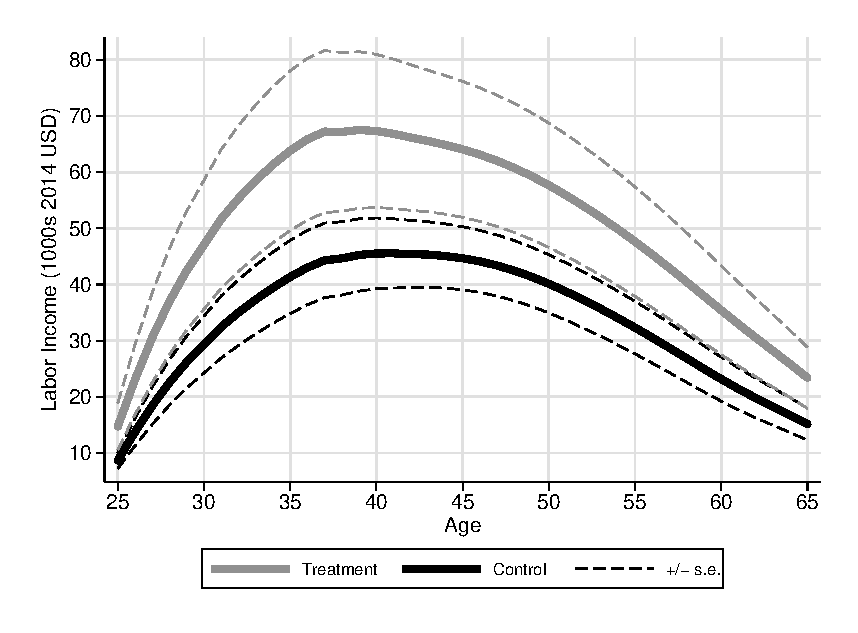
\includegraphics[width=.55\textwidth]{output/labor_25-65_pset1_mset3_male.eps}
\end{center}
\tiny \flushleft Note: This figure displays the predicted life-cycle labor income profiles for ABC/CARE males by treatment status, based on the method proposed in this section. We combine data from the Panel Study of Income Dynamics (PSID), the National Longitudinal Survey of Youth 1979 (NLSY79), and the Children of the National Longitudinal Survey of Youth 1979 (CNLSY79). We highlight the \textit{observed} labor income at $a^*$ (age 30) for the ABC/CARE control- and treatment-group participants.\\
\end{figure}

\end{frame}

%% ------------------------------------------------------------------------------------------------
\begin{frame}

\begin{figure}[H]\addtocounter{figure}{-1}
\caption{Predicted Labor Income Profiles for ABC/CARE Participants, Females}\label{fig:labor-income-profilesa}
\begin{center}
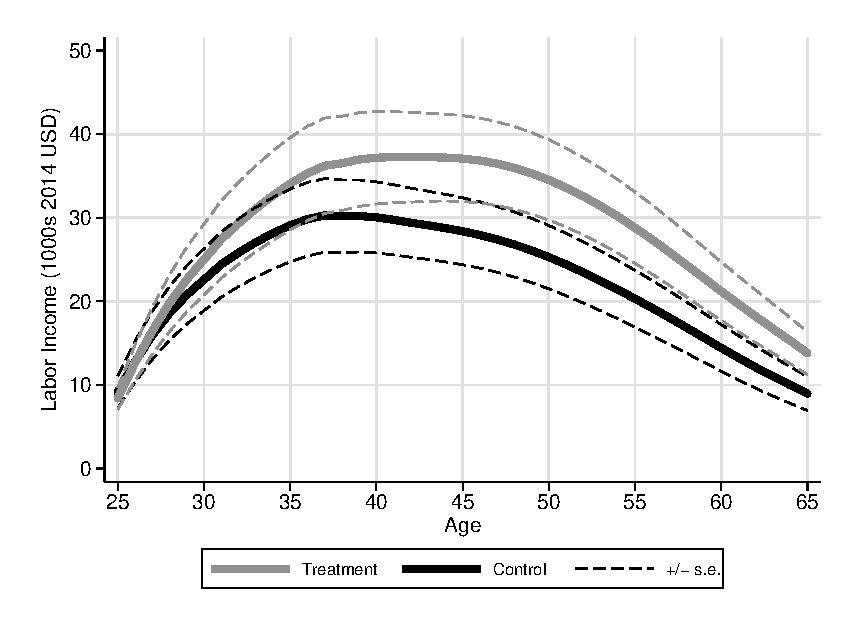
\includegraphics[width=.65\textwidth]{output/labor_25-65_pset1_mset3_female.eps}
\end{center}
\tiny \flushleft Note: This figure displays the analogous figure for females. Our predictions go up to age 67, age of assumed retirement. Standard errors are based on the empirical bootstrap distribution. We combine data from the Panel Study of Income Dynamics (PSID), the National Longitudinal Survey of Youth 1979 (NLSY79), and the Children of the National Longitudinal Survey of Youth 1979 (CNLSY79). We highlight the \textit{observed} labor income at $a^*$ (age 30) for the ABC/CARE control- and treatment-group participants.\\
\end{figure}

\end{frame}

%% ------------------------------------------------------------------------------------------------
\begin{frame}

\begin{itemize}
\item A test of the validity of our procedures.
\item In the experimental sample all of the parents of children with characteristics $\bm{B} \in \mathcal{B}_0$ agree to participate in the program.
\item Because the auxiliary samples have no treatment group members, we can evaluate our procedure by comparing the labor incomes of individuals in the auxiliary samples for whom $\bm{B} \in \mathcal{B}_0$ to the labor incomes of individuals in our constructed synthetic control group.
\item Figure~\ref{figure:controltests} makes this comparison.
\end{itemize}

\end{frame}

\textbf{[JJH: In slides says Figure 7, here it is Figure 8---why?] [Typist: My guess is that it ``counts'' figures that are only in notes and thus ups the count in notes-only---how interesting!]}

\begin{itemize}
\item Note we do not condition on education
\end{itemize}

\clearpage
%% ------------------------------------------------------------------------------------------------
\begin{frame}

\begin{figure}[H]
\caption{Labor Income Profile, Disadvantaged Individuals Synthetic Control Group in the Auxiliary Samples, Males}\label{figure:controltests}
\begin{center}
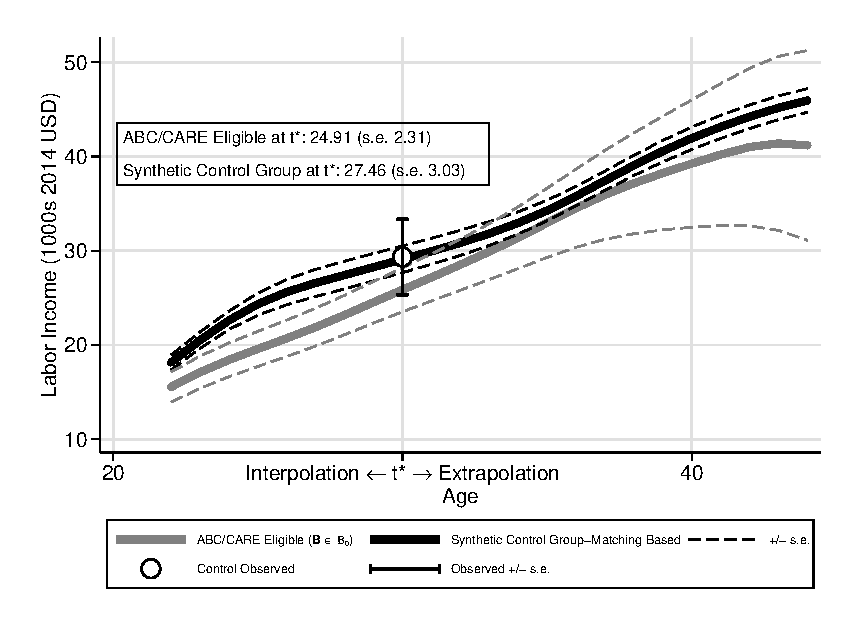
\includegraphics[width=.65\textwidth]{output/abccare_disad_1}
\end{center}
\tiny \flushleft Note: This figure displays the predicted labor income for males in the auxiliary samples for whom $\bm{B} \in \mathcal{B}_0$, i.e. ABC/CARE eligible, and for the synthetic control group we construct based on the method proposed in this section. We combine data from the Panel Study of Income Dynamics (PSID), the National Longitudinal Survey of Youth 1979 (NLSY79), and the Children of the National Longitudinal Survey of Youth 1979 (CNLSY79). We highlight the observed labor income at $a^*$ (age 30) for the ABC/CARE control- and treatment-group participants. We stop at age 45 for want of data to compute the High-Risk Index defining $\bm{B} \in \mathcal{B}_0$ in the auxiliary samples.\\
\end{figure}

\end{frame}

%% ------------------------------------------------------------------------------------------------
\begin{frame}

\begin{figure}[H]\addtocounter{figure}{-1}
\caption{Labor Income Profile, Disadvantaged Individuals Synthetic Control Group in the Auxiliary Samples, Females}\label{figure:controltests}
\begin{center}
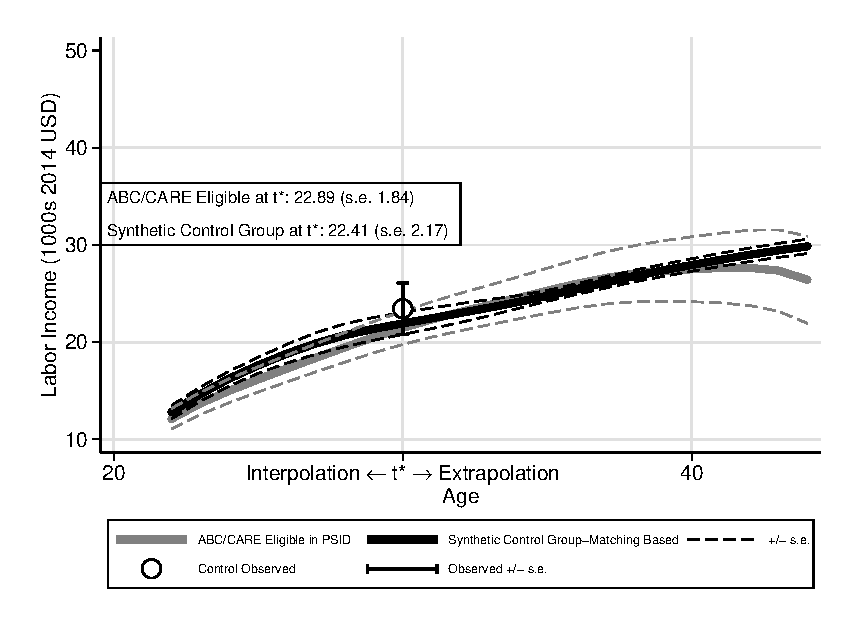
\includegraphics[width=.65\textwidth]{output/abccare_disad_0}
\end{center}
\tiny \flushleft Note: This figure displays the analogous figure for females. Standard errors are based on the empirical bootstrap distribution. We combine data from the Panel Study of Income Dynamics (PSID), the National Longitudinal Survey of Youth 1979 (NLSY79), and the Children of the National Longitudinal Survey of Youth 1979 (CNLSY79). We highlight the observed labor income at $a^*$ (age 30) for the ABC/CARE control- and treatment-group participants. We stop at age 45 for want of data to compute the High-Risk Index defining $\bm{B} \in \mathcal{B}_0$ in the auxiliary samples.\\
\end{figure}

\end{frame}

%% ------------------------------------------------------------------------------------------------
\begin{frame}

\begin{center}
\textbf{Constructing Out-of-Sample Forecasts}
\end{center}

\end{frame}

%% ------------------------------------------------------------------------------------------------
\begin{frame}

\begin{center}
\textbf{Analytical Framework}
\end{center}

\end{frame}

%% ------------------------------------------------------------------------------------------------
\begin{frame}

\begin{itemize}
\item Causal model for treatment ($d=1$) and control ($d=0$)
\item Outcome $j$, in sample $k$, at age $a$, for measure $j$ at age $a$ in sample $k \in \{e,n\}$
\item $e$: membership in the experimental sample
\item $n$: membership in the auxiliary sample:
\end{itemize}

\begin{equation}\label{eq:outcome}
Y^d_{k,j,a} = \phi^d_{k,j,a} (\bm{X}^d_{k,a}, \bm{B}_k) + \varepsilon^d_{k,j,a}, \quad j \in \mathcal{J}_a.
\end{equation}

\end{frame}

%% ------------------------------------------------------------------------------------------------
\begin{frame}

\begin{itemize}
\item $\phi^d_{k,j,a}\left( \cdot, \cdot \right)$: \textbf{policy-invariant structural production function}.
\item Normalize $\varepsilon^d_{k,j,a}$ to have mean zero.
\item Among the $\bm{X}^d_{k,a}$: variables caused by treatment and lagged dependent variables.
\item $\bm{Y}_k^d$: all outcomes $a\in\{1,\dots,A\}$ for $k \in \{e, n \}$, when treatment status is fixed to $d$.
\item $\bm{X}_k^d$: vector of all causal predictors of $\bm{Y}_k^d$ at all ages.
\item Background variables $\bm{B}$ may have different distributions in the two samples.
\end{itemize}

\end{frame}

%% ------------------------------------------------------------------------------------------------
\begin{frame}

\begin{itemize}
\item Joint distribution conditional on: $\bm{B}_k = \bm{b}$: $F_{\bm{Y}_k^d, \bm{X}_k^d | \bm{B}_k = \bm{b}}(\cdot,\cdot)$.
\item Can use $D_e$ and $R_e$ interchangeably (because of full compliance).
\item Standard \citet{Quandt_1972_JASA} switching regression model:
\end{itemize}

\mode<presentation>{\begin{small}}
\mode<article>{\begin{large}}
\begin{align}\label{eq:countersystem}
Y_{k,j,a} =& \left( 1 - D_k \right) Y_{k,j,a}^0 + \left( D_k \right) Y_{k,j,a}^1, \\
&&j \in \mathcal{J}_a, a \in \{1,\dots,A\}, \quad k \in \{e,n\} \nonumber \\
\bm{X}_{k,a} =& \left( 1 - D_k \right) \bm{X}_{k,a}^0 + \left( D_k \right) \bm{X}_{k,a}^1. \nonumber
\end{align}
\mode<article>{\end{large}}
\mode<presentation>{\end{small}}

\end{frame}

%% ------------------------------------------------------------------------------------------------
\begin{frame}

\begin{center}
\textbf{Accounting for Age, Period, and Cohort Effects}
\end{center}

\end{frame}

%% ------------------------------------------------------------------------------------------------
\begin{frame}

\mode<presentation>{\begin{footnotesize}}
\begin{itemize}
\item To formalize problem, let $Y_{j,k,a,c,t}^d$ be outcome $j$ for sample $k$ at age $a$ for birth cohort $c$ at time $t$ when treatment is fixed to $d$.
\end{itemize}

\begin{assumption}\label{ass:alignment} \textbf{Alignment of Cohort and Time Effects}\\
For experimental sample cohort $c_{e}$ and auxiliary sample cohort $c_{n}$:
\begin{equation}
Y_{e,a,c_{e},t_{e}}^d = Y_{n,a,c_{n},t_{n}}^d
\end{equation}
for $d \in \{ 0, 1\}$, $a \geq a^*$, where $t_{e}, t_{n}$ are the years for which cohorts $c_{e}, c_{n}$ are observed, where $t_e = t_n + c_e - c_n$, and $t_n$ is the year that the age $a$ outcome is observed for cohort $n$ ($t_n = a + c_n$). $\square$
\end{assumption}

\mode<presentation>{\end{footnotesize}}

\end{frame}

%% ------------------------------------------------------------------------------------------------
\begin{frame}

\begin{itemize}
\item Cohort and time effects assumed to operate identically across the $e$ and $n$ samples.
\item Does \textbf{not} assume the absence of cohort and time effects, just similarity.
\item We adjust estimates for plausible cohort effects in health, earnings, etc.
\end{itemize}

\end{frame}

%% ------------------------------------------------------------------------------------------------
\begin{frame}

\begin{center}
\textbf{Support Conditions}
\end{center}

\end{frame}

%% ------------------------------------------------------------------------------------------------
\begin{frame}

\begin{assumption} \label{ass:contain} \textbf{Support Conditions} \\
For $a \in \{ 1, \ldots, A \}$, the support of $\left( \bm{Y}^d_{e,a}, \bm{X}^d_{e,a}, \bm{B}_e \right)$ in the experimental sample is contained in the support of $\left( \bm{Y}^d_{n,t}, \bm{X}^d_{n,t}, \bm{B}_e \right)$ in the auxiliary sample:
\begin{equation}
supp( \bm{Y}_{e,a}, \bm{X}^d_{e,a}, \bm{B}_e ) \subseteq supp( \bm{Y}_{n,a}, \bm{X}^d_{n,a}, \bm{B}_n ), \quad d \in \{0,1\}. \quad \square
\end{equation}
\end{assumption}

\begin{itemize}
\item Can test for ages $a\leq a^\ast$.
\item Condition satisfied in our samples.
\end{itemize}

\end{frame}

%% ---------------------------------------------------------------------------
\begin{frame}

\hypertarget{ret:doughnut}{}
\begin{center}
\hyperlink{doughnut}{\underline{Link to Appendix:}}\\
Common Support between Experimental\\ and Non-Experimental Samples
\end{center}

\end{frame}

%% ------------------------------------------------------------------------------------------------
\begin{frame}

\begin{center}
\textbf{Various Conditions for Valid Out-of-Sample Predictions}
\end{center}

\end{frame}

%% ------------------------------------------------------------------------------------------------
\begin{frame}

\begin{itemize}
\item Standard in ``surrogate marker'' literature (see \citealp{Prentice_1989_Surrogate_SiM}; Little 2004)
\end{itemize}

\end{frame}

%\textbf{[Typist: Professor, what is the title/other authors on the Little paper so we can add it to the bib?]} <-- lol I tried keeping it here for a reminder

%% ------------------------------------------------------------------------------------------------
\begin{frame}

\begin{condition} \textbf{Equality of Distributions Across the Experimental and Auxiliary Samples \label{cond:cond1}}
\begin{equation}
F_{\bm{Y}_e^d, \bm{X}_e^d | \bm{B}_e = \bm{b}} \left( \cdot, \cdot \right) = F_{\bm{Y}_n^d, \bm{X}_n^d | \bm{B}_n = \bm{b}} \left( \cdot, \cdot \right), \quad d \in \{0,1\}
\end{equation}
\noindent for $\bm{Y}_e^d, \bm{X}^d_e | \bm{B}_e = \bm{b}$ and $\bm{Y}_n^d, \bm{X}^d_n | \bm{B}_n = \bm{b}$ contained the support of the experimental sample $supp\left(\bm{Y}^d_{e}, \bm{X}^d_{e}, \bm{B}\right)$.
\end{condition}

\end{frame}

%% ------------------------------------------------------------------------------------------------

\begin{itemize}
\item Strongly sufficient
\end{itemize}

%% ------------------------------------------------------------------------------------------------
\begin{frame}

\begin{condition} \textbf{Equality in Conditional Expectations Across the Experimental and Auxiliary Samples \label{cond:cond2}}
\begin{equation}
\mathbb{E} \left[ \bm{Y}_e^d |  \bm{X}_e^d = \bm{x}, \bm{B}_e = \bm{b} \right] = \mathbb{E} \left[ \bm{Y}_n^d |  \bm{X}_n^d = \bm{x}, \bm{B}_n = \bm{b} \right], \quad d \in \{0,1\}
\end{equation}
for $d \in \{0, 1 \}$ over $supp\left(\bm{Y}^d_{e,a}, \bm{X}^d_{e,a}, \bm{B}_e\right)$.
\end{condition}

\end{frame}

%% ------------------------------------------------------------------------------------------------
\begin{frame}

\begin{condition} \textbf{Equality in Mean Treatment Effects \\Across the Experimental and Auxiliary Samples}\label{cond:cond3}
\begin{equation}
\mathbb{E} \left[ \bm{Y}_e^1 - \bm{Y}_e^0 | \bm{B}_e = \bm{b} \right] = \mathbb{E} \left[ \bm{Y}_n^1 - \bm{Y}_n^0 | \bm{B}_n = \bm{b} \right]
\end{equation}
over $supp\left(\bm{Y}^d_{e,a}, \bm{B}_e\right)$.
\end{condition}

\begin{itemize}
\item Minimal requirement for valid age by age forecasts (necessary and sufficient)
\end{itemize}

\end{frame}

%% ------------------------------------------------------------------------------------------------
\begin{frame}

\begin{itemize}
\item We could simply invoke Condition~\ref{cond:cond2} or \ref{cond:cond3} and be done.
\item Our approach is to examine Condition~\ref{cond:cond2} and test (when possible) assumptions that justify it.
\end{itemize}

\end{frame}

%% ------------------------------------------------------------------------------------------------
\begin{frame}

\begin{center}
\textbf{Exogeneity}
\end{center}

\end{frame}

%% ------------------------------------------------------------------------------------------------
\begin{frame}

\begin{assumption}\label{ass:exog} \textbf{Exogeneity}\\
For all $a, a'' \in \{ 1, \ldots, A \}$ and for $d, d' \in \{0,1\}$,
\begin{equation}
\varepsilon^d_{k,j,a} \indep \bm{X}^{d^{\prime}}_{k,a^{''}} | \bm{B}_k = \bm{b}
\end{equation}
for all $\bm{b}$ in the support of $\bm{B}_k, \: k \in \{e,n\}$, for all outcomes $j \in \mathcal{J}_{a}$, where ``$\bm{M} \indep \bm{N}|\bm{Q}$'' denotes independence of $\bm{M}$ and $\bm{N}$ given $\bm{Q}$. $\square$
\end{assumption}

\end{frame}

%% ------------------------------------------------------------------------------------------------
\begin{frame}

\begin{itemize}
\item Exogeneity facilitates the use of economic theory to generate and interpret treatment effects, to test the validity of our synthetic control groups, and to find auxiliary sample counterparts to treatments and controls.
\item However, it is \textbf{not} essential to our approach.
\item We relax and test it using a variety of specifications.
\end{itemize}

\end{frame}

%% ---------------------------------------------------------------------------
\begin{frame}

\hypertarget{ret:tarttarttart}{}
\begin{center}
\hyperlink{tarttarttart}{\underline{Link to Appendix:}}\\
\vspace{1.5mm}
Tests of Exogeneity
\end{center}

\end{frame}

%% ---------------------------------------------------------------------------
\begin{frame}

\begin{itemize}
\item Useful starting point to focus on main ideas
\item We start with exogeneity and relax this assumption using a variety of panel data estimation methods
\end{itemize}

\end{frame}

%% ------------------------------------------------------------------------------------------------
\begin{frame}

\begin{center}
\textbf{Structural Invariance}
\end{center}

\end{frame}

%% ------------------------------------------------------------------------------------------------
\begin{frame}

\begin{assumption} \label{ass:summary} \textbf{Structural Invariance}\\
For all $\bm{x}, \bm{b} \in supp(\bm{X}^d_{e,a}, \bm{B}_e), k \in \{e,n\}$
\begin{align}
\phi_{k,j,a}^0 \left( \bm{x}, \bm{b} \right) &= \phi_{k,j,a}^1 (\bm{x}, \bm{b}) \\   \nonumber
                                                                     &=: \phi_{j,a} (\bm{x}, \bm{b}),
\end{align}
$\phi^d_{k,j,a}(\bm{x})$ is the function generating the causal effect of setting $\bm{X}^d_{k,a}=\bm{x}$ holding $\varepsilon^d_{k,j,a}$ fixed for $a \in \{1,\dots,A\}$ for any outcome $j \in \mathcal{J}_{a}$. $\square$
\end{assumption}

\begin{itemize}
\item (\citealp{Frisch_1938_autonomy,Hurwicz_1962_structural})
\end{itemize}

\end{frame}

%% ------------------------------------------------------------------------------------------------
\begin{frame}

\begin{itemize}
\item Two distinct messages of \ref{ass:summary}:
    \begin{enumerate}[(i)]
    \item Structural functions evaluated at the same arguments have identical values for treatment and control groups in the experimental sample.
    \item Structural relationships are identical in the experimental and auxiliary samples.
    \end{enumerate}
\end{itemize}

\end{frame}

%% ------------------------------------------------------------------------------------------------
\begin{frame}

\begin{center}
\textbf{Testable Implications}
\end{center}

\end{frame}

%% ------------------------------------------------------------------------------------------------
\begin{frame}

\begin{align}\label{eq:withbetimplication}
&\mathbb{E} \left[ Y_{e,j,a} | \bm{X}^d_{e,a} = \bm{x}, \bm{B}_e = \bm{b} \right] = \mathbb{E} \left[ Y_{n,j,a} | \bm{X}^d_{n,a} = \bm{x}, \bm{B}_e = \bm{b} \right]\\
& \quad d \in \{0,1\} \quad  a \in \{1,\dots,A\}. \nonumber
\end{align}

\begin{itemize}
\item Relationship~\eqref{eq:withbetimplication} testable for $a \leq  a^*$, when $Y_{k,j,a}$ is observed in both the experimental and auxiliary samples.
\item We fail to reject the null hypotheses of no differences in the conditional mean functions in the experimental and auxiliary samples.
\end{itemize}

\end{frame}

%% ------------------------------------------------------------------------------------------------
\begin{frame}

\begin{equation}\label{eq:invariancetest}
\mathbb{E} \left[ Y_{k,j,a}^d | \bm{X}_{k,a}^d  = \bm{x}, \bm{B}_k = \bm{b}, D = d \right] = \mathbb{E} \left[ Y_{k,j,a} | \bm{X}^d_{k,a}  = \bm{x}, \bm{B}_k = \bm{b} \right]
\end{equation}

\begin{itemize}
\item Can test \eqref{eq:invariancetest} within the experimental sample ($a \leq a^*$).
\end{itemize}

\end{frame}

%% ---------------------------------------------------------------------------
\begin{frame}

\hypertarget{ret:creamcheese}{}
\begin{center}
\hyperlink{creamcheese}{\underline{Link to Appendix:}}\\
\vspace{1.5mm}
Tests of Implications
\end{center}

\end{frame}

%% ------------------------------------------------------------------------------------------------
\begin{frame}

\setcounter{theorem}{0}
\begin{theorem}\label{theorem:main} \textbf{Valid Out-of-Sample Predictions} \\
Under Assumptions~\ref{ass:alignment}-\ref{ass:summary}, Conditions~\ref{cond:cond1} through \ref{cond:cond3} hold for any value of $\left( \bm{X}^d_{k,a}, \bm{B}_k \right)$. \\
\emph{This is an immediate consequence of the cited assumptions.} $\Box$
\end{theorem}

\end{frame}

%% ---------------------------------------------------------------------------
\begin{frame}

\hypertarget{ret:candycane}{}
\begin{center}
\hyperlink{candycane}{\underline{Link to Appendix:}}\\
Exploring the Impact of Using Different Prediction Models
\end{center}

\end{frame}

%% ---------------------------------------------------------------------------
\begin{frame}

\begin{itemize}
\item Alternative intuitive approach: \textbf{matching}.
\item Under exogeneity of $\bm{X}$, matching constructs control and treatment groups.
\item Potential danger: endogeneity in the auxiliary samples.
\item We compare our estimates from various procedures.
\end{itemize}

\hypertarget{ret:potpie}{}
\begin{center}
\hyperlink{potpie}{\underline{Link to Appendix:}}\\
Using Matching to Construct Virtual \\ Treatment and Comparison Groups
\end{center}

\end{frame}

\textbf{[JJH: Jorge, we need a link to the matching appendix---explain Algorithm 1 for example] [JLG: the link above has bene updated and contains the discussion]}

%% ---------------------------------------------------------------------------
\begin{frame}

\begin{center}
\textbf{Health}
\end{center}

\begin{itemize}
\item Future America Model (FAM).
\item Projects health outcomes from the subjects' mid-30s up to their projected death \citep{Goldman_etal_2015_Future-Elderly-Model-Report}
\end{itemize}

\end{frame}

%% ---------------------------------------------------------------------------

\begin{frame}

\begin{figure}[H]
\caption{Abecedarian Project, Health Effects at Age 34 (Males)}
\begin{center}
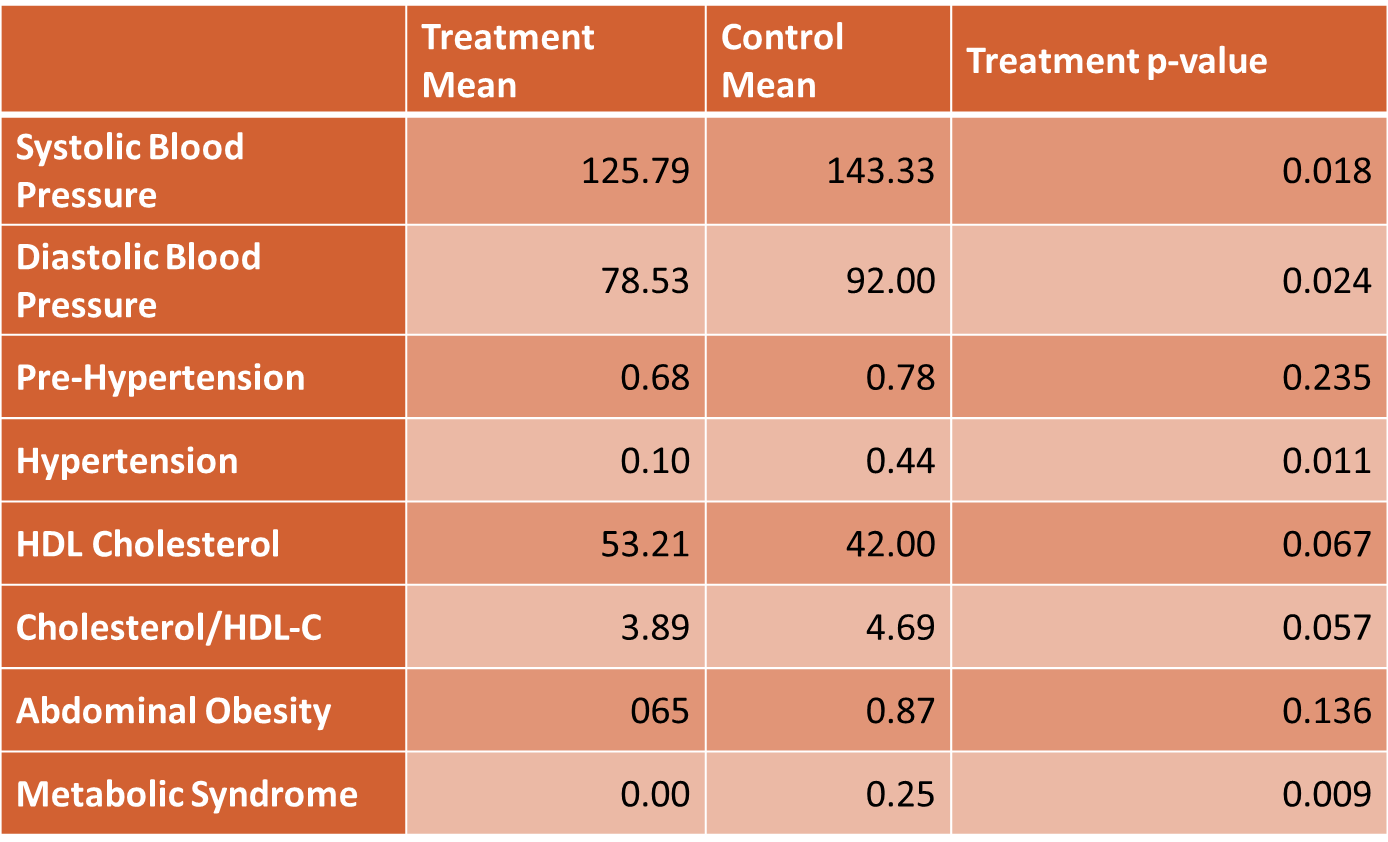
\includegraphics[width=0.9\textwidth]{include/ABC-Health-Effects-Age-35.png}
\end{center}
{\flushleft \scriptsize \emph{Source}: Campbell, Conti, Heckman, Moon, Pinto, Pungello, and Pan (2014).\\}
\end{figure}

\end{frame}

%% ---------------------------------------------------------------------------
\begin{frame}

\begin{itemize}
\item Five steps:
    \begin{enumerate}[(1)]
    \item Estimate age-by-age health state transition probabilities using the Panel Study of Income Dynamics (PSID);
    \item Match these transition probabilities to the ABC/CARE subjects based on observed characteristics;
    \item Estimate quality-adjusted life year (QALY) models using the Medical Expenditure Panel Survey (MEPS) and the PSID;
    \item Estimate medical cost models using the MEPS and the Medicare Current Beneficiary Survey (MCBS), allowing estimates to differ by health state and observed characteristics;
    \item Predict the medical expenditure and QALYs that correspond to the simulated individual health trajectories
    \end{enumerate}
\end{itemize}

\end{frame}


\clearpage
%% ---------------------------------------------------------------------------
\begin{frame}

\begin{table}[H]
\caption{Health State Transitions, Age $a$ as Predictor of Age $a+1$}\label{table:transition}
\mode<presentation>{\begin{scriptsize}}
\begin{center}
\begin{tabular}{l|ccccccc} \toprule
\multicolumn{1}{c}{Age $a$} & \multicolumn{7}{c}{Age $a+1$} \\ \midrule
  & Heart & Hyper- & Stroke & Lung  & Diabetes & Cancer & Disability \\
&  Disease & tension &  & Disease & & & \\
Heart Disease & & & $\times$& & & &$\times$ \\
Hypertension  &  $\times$& & $\times$ & & & &$\times$ \\
Stroke           & & & & & & &$\times$ \\
Lung Disease & & & & & & &$\times$ \\
Diabetes       & $\times$ &$\times$  & $\times$   & & & &$\times$ \\
Cancer         & & & $\times$ &  & &   &$\times$ \\
Disability     & & & & & & &$\times$ \\
\midrule
Smoking & $\times$& $\times$ & $\times$ & $\times$& $\times$& $\times$&$\times$ \\
BMI & $\times$& $\times$&$\times$ & $\times$& $\times$& $\times$&$\times$ \\
Physical Activ. & $\times$& $\times$&$\times$ & $\times$& $\times$& $\times$&$\times$ \\
Binge Drinking & & & & & & &  \\
\midrule
DI Claim      & & & & &  & & \\
SS Claim     & & & & & & & \\
SSI Claim   & & & & & & & \\ \bottomrule
\end{tabular}
\end{center}
\mode<presentation>{\end{scriptsize}}
\end{table}

\end{frame}

%% ---------------------------------------------------------------------------
\begin{frame}

\begin{table}[H]
\addtocounter{table}{-1}
\caption{Health State Transitions, Age $a$ as Predictor of Age $a+1$, Cont.}\label{table:transition}
\mode<presentation>{\begin{scriptsize}}
\begin{center}
\begin{tabular}{l|ccccccc} \toprule
\multicolumn{1}{c}{Age $a$} & \multicolumn{7}{c}{Age $a+1$} \\ \midrule
& Mortality & Smoking  & Obesity & Health  & DI  & SS  & SSI  \\
& &  &  & Insurance & Claim & Claim & Claim \\
Heart Disease &$\times$ & $\times$           &       &  $\times$  & $\times$ & $\times$ & $\times$\\
Hypertension  &$\times$ &       &     & $\times$   & $\times$ & $\times$  & $\times$\\
Stroke          &$\times$ &             &      &   $\times$  & $\times$ & $\times$  & $\times$\\
Lung Disease  &$\times$ & $\times$    &        &   $\times$  &$\times$  & $\times$  & $\times$\\
Diabetes      &$\times$ & $\times$            &       &  $\times$    & $\times$& $\times$ & $\times$ \\
Cancer        & $\times$&           &         &   $\times$  & $\times$ & $\times$  & $\times$\\
Disability    &$\times$ &         &      &     $\times$  & $\times$ & $\times$   & $\times$\\
\midrule
Smoking &$\times$ & $\times$   &   &     $\times$  & $\times$ & $\times$   & $\times$\\
BMI   & & $\times$    &  $\times$ &     &  &   & \\
Physical Activ.  & & $\times$    &   &     &   &  & \\
Binge Drinking  &$\times$ & $\times$    &      &      &   &     &  \\
\midrule
DI Claim     & &             &         & $\times$    & $\times$   & $\times$ & $\times$\\
SS Claim     &           &         &     & $\times$ &  & $\times$& $\times$\\
SSI Claim    & &         &        &      & &   & $\times$\\ \bottomrule
\end{tabular}
\end{center}
\mode<presentation>{\end{scriptsize}}
\end{table}

\end{frame}

{\flushleft \normalsize This table illustrates how health outcomes at age a predict health outcomes at age a + 1. The crosses indicate if we use the age a outcome to predict the age a + 1 outcome. DI Claim: payroll-tax funded, federal insurance program for individuals who work long enough paying social security taxes; SS Claim: old-age survivors and disability insurance program collected through payroll taxes by the Internal Revenue Service; SSI Claim: claims of stipends for low-income people who are older than 65 years old, blind, or disabled.\\}

%% ---------------------------------------------------------------------------
\begin{frame}

\begin{figure}[H]
\caption{Quality Adjusted Life Years, Predictions and Comparison to PSID}\label{fig:qalys}
\begin{center}
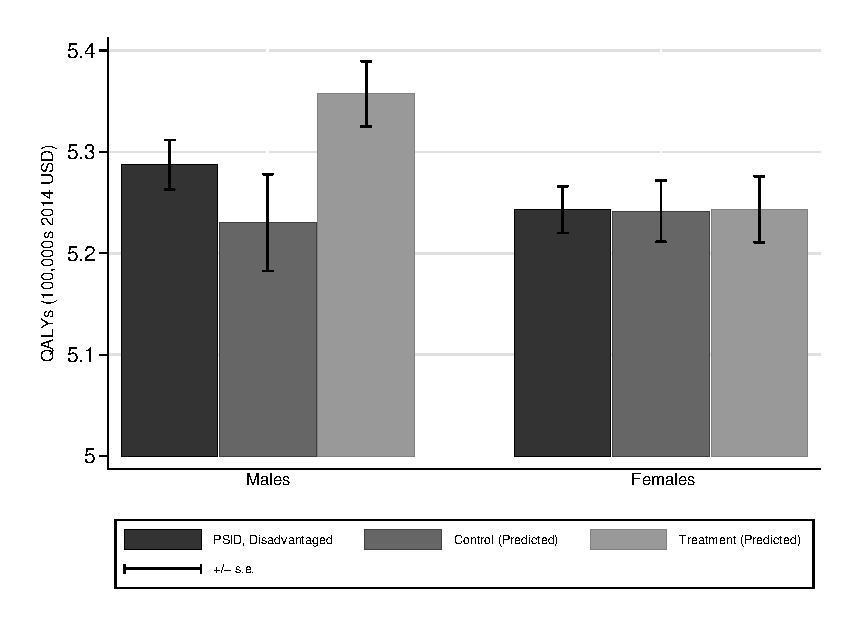
\includegraphics[width=.85\columnwidth]{output/qalyexppsid.eps}
\end{center}
\end{figure}

\end{frame}

{\flushleft \normalsize Note:  This figure displays the life-cycle net-present value of predicted quality-adjusted life years (QALYs) for ABC/CARE males and females, respectively, by treatment status. The predictions are based on combining data from the Panel Study of Income Dynamics (PSID), the Health Retirement Study, and the Medical Expenditure Panel Survey (MEPS). For each gender, we display a comparison to disadvantaged males and females in the Panel Study of Income Dynamics (PSID), where disadvantaged is defined as being Black and having 12 years of education or less. QALYs are the quality-adjusted life years gain due to better health conditions. Standard errors are based on the empirical bootstrap distribution.\\}
\clearpage
%% ---------------------------------------------------------------------------
\begin{frame}

\begin{center}
\textbf{Crime}
\end{center}

\end{frame}

%% ---------------------------------------------------------------------------
\begin{frame}

\hypertarget{ret:muffin}{}
\begin{center}
\hyperlink{muffin}{\underline{Link to Appendix: Quantifying the Benefits in Crime Reduction}}
\end{center}

\end{frame}

%% ---------------------------------------------------------------------------
\begin{frame}

\begin{block}{}
\begin{center}
\textbf{Putting It All Together: Benefit/Cost and Rate of Return Analysis}
\end{center}
\end{block}

\end{frame}

%% ---------------------------------------------------------------------------
\begin{frame}

\begin{center}
\textbf{Program Costs}
\end{center}

\begin{itemize}
\item The yearly cost of the program: \$18,514 per participant (2014 USD).
\end{itemize}

\end{frame}
%% ---------------------------------------------------------------------------
\begin{frame}

\begin{figure}[H]
\caption{Life-cycle Net Present Value of Main Components of the CBA}\label{fig:npvsgender}
\begin{center}
\begin{tabular}{c}
(a) Males\\
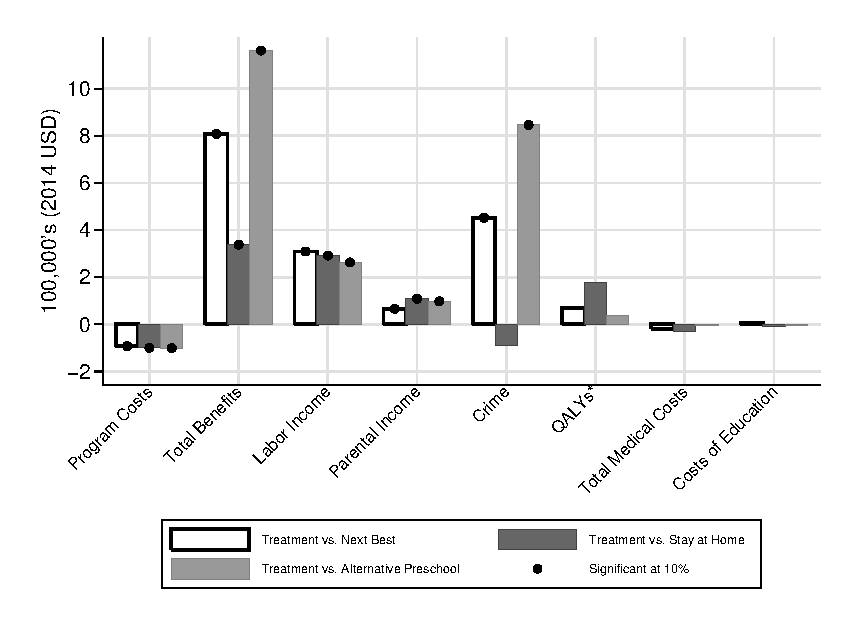
\includegraphics[width=0.75\textwidth]{output/abccare_npvs2.eps}
\end{tabular}
\end{center}
\end{figure}

\end{frame}

\clearpage

{\flushleft \small Note: This figure displays the life-cycle net present values of the main components of the cost/benefit analysis of ABC/CARE from birth to predicted death, discounted to birth at a rate of 3\%. ``Treatment vs. Control'': compares the treatment to the control group. ``Treatment vs. Stay at Home'': compares the treatment group to those subjects who stayed at home. ``Treatment vs. Alternative Preschool'': compares the treatment group to those subjects who attended alternative preschools. The latter two are based on matching estimators that account for selection on observable variables. By ``net" we mean that each component represents the total value for the treatment group minus the total value for the control group. Program costs: the total cost of ABC/CARE, including the welfare cost of taxes to finance it. Total net benefits: are for \textit{all} of the components we consider. Labor income: total individual labor income from ages 20 to the retirement of program participants (assumed to be age 67). Parental income: total parental labor income of the parents of the participants from when the participants were ages 1.5 to 21. Crime: the total cost of crime (judicial and victimization costs). To simplify the display, the following components are not shown in the figure: (i) cost of alternative preschool paid by the control group children parents; (ii) the social welfare costs of transfer income from the government; (iii) disability benefits and social security claims; (iv) costs of increased individual and maternal education (including special education and grade retention); (v) total medical public and private costs. Inference is based on non-parametric, one-sided $p$-values from the empirical bootstrap distribution. We indicate point estimates significant at the $10\%$ level.\\
*The treatment vs. stay at home net present value is sizable and negative (-\$91,476.3); its standard error is \$86,657.3.\\
**QALYs refers to the quality-adjusted life years. Any gain corresponds to better health conditions until predicted death, with $\$150,000$ (2014 USD) as base value for a year of life.\\}

\clearpage
%% ---------------------------------------------------------------------------
\begin{frame}

\begin{figure}[H]
\addtocounter{figure}{-1}
\caption{Life-cycle Net Present Value of Main Components of the CBA, Cont'd}\label{fig:npvsgender}
\begin{center}
\begin{tabular}{c}
(b) Females\\
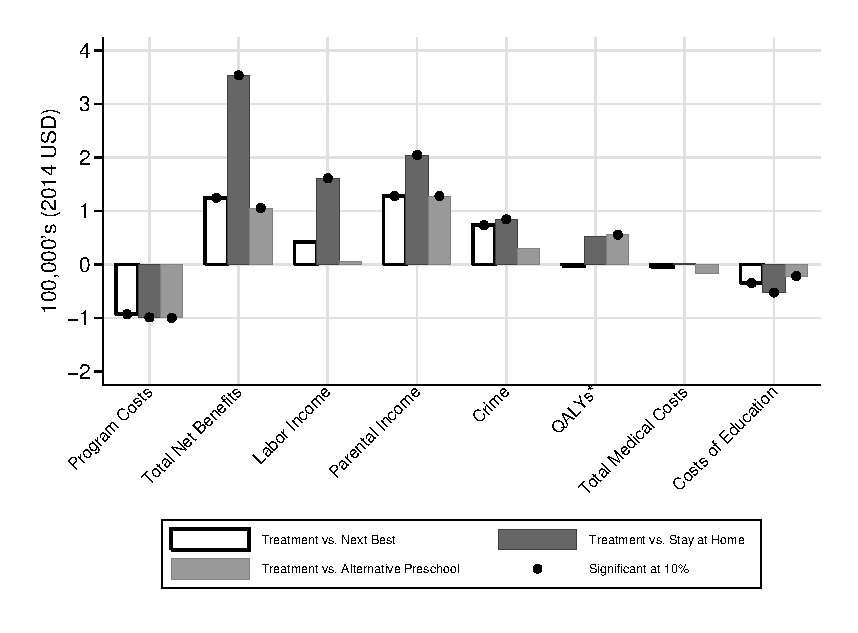
\includegraphics[width=0.75\textwidth]{output/abccare_npvs1.eps}
\end{tabular}
\end{center}
\end{figure}

\end{frame}

\clearpage

{\flushleft \small Note: This figure displays the life-cycle net present values of the main components of the cost/benefit analysis of ABC/CARE from birth to predicted death, discounted to birth at a rate of 3\%. ``Treatment vs. Control'': compares the treatment to the control group. ``Treatment vs. Stay at Home'': compares the treatment group to those subjects who stayed at home. ``Treatment vs. Alternative Preschool'': compares the treatment group to those subjects who attended alternative preschools. The latter two are based on matching estimators that account for selection on observable variables. By ``net" we mean that each component represents the total value for the treatment group minus the total value for the control group. Program costs: the total cost of ABC/CARE, including the welfare cost of taxes to finance it. Total net benefits: are for \textit{all} of the components we consider. Labor income: total individual labor income from ages 20 to the retirement of program participants (assumed to be age 67). Parental income: total parental labor income of the parents of the participants from when the participants were ages 1.5 to 21. Crime: the total cost of crime (judicial and victimization costs). To simplify the display, the following components are not shown in the figure: (i) cost of alternative preschool paid by the control group children parents; (ii) the social welfare costs of transfer income from the government; (iii) disability benefits and social security claims; (iv) costs of increased individual and maternal education (including special education and grade retention); (v) total medical public and private costs. Inference is based on non-parametric, one-sided $p$-values from the empirical bootstrap distribution. We indicate point estimates significant at the $10\%$ level.\\
*The treatment vs. stay at home net present value is sizable and negative (-\$91,476.3); its standard error is \$86,657.3.\\
**QALYs refers to the quality-adjusted life years. Any gain corresponds to better health conditions until predicted death, with $\$150,000$ (2014 USD) as base value for a year of life.\\}

\clearpage

%% ---------------------------------------------------------------------------
\begin{frame}[shrink=10]

\begin{table}[H]
\caption{Cost/benefit Analysis of ABC/CARE, Summary}\label{table:cba}
\begin{center}
\mode<presentation>{\begin{tiny}}
\mode<article>{\begin{scriptsize}}
\begin{tabular}{l r r r r r r r r r}																			
\toprule																			
&       \mc{3}{c}{Females}      &       \mc{3}{c}{Males}        &       \mc{3}{c}{Pooled}       \\																			
\cmidrule(lr){2-4}      \cmidrule(lr){5-7}      \cmidrule(lr){8-10}																			
Removed Component       &       NPV     &       IRR     &       B/C     &       NPV     &       IRR     &       B/C     &       NPV     &       IRR     &       B/C     \\																			
\midrule																			
None	&	161,759	&	\textbf{10.1\%}	&	\textbf{2.61}	&	919,049	&	\textbf{14.7\%}	&	\textbf{10.19}	&	636,674	&	\textbf{13.7\%}	&	\textbf{7.33}	\\
	&		&	(6\%)	&	(0.73)	&		&	(4\%)	&	(2.93)	&		&	(3\%)	&	(1.84)	\\ \\
Parental Income	&	148,854	&	4\%	&	1.12	&	107,907	&	\textbf{11\%}	&	\textbf{9.10}	&	116,953	&	\textbf{9\%}	&	\textbf{6.17}	\\
	&		&	(2\%)	&	(0.65)	&		&	(3\%)	&	(2.92)	&		&	(3\%)	&	(1.87)	\\
Subject Labor Income	&	41,908	&	9\%	&	\textbf{2.21}	&	238,105	&	\textbf{13\%}	&	\textbf{7.75}	&	133,032	&	\textbf{13\%}	&	\textbf{6.03}	\\
	&		&	(6\%)	&	(0.66)	&		&	(5\%)	&	(2.23)	&		&	(4\%)	&	(1.77)	\\
Subject Transfer Income	&	419	&	\textbf{10\%}	&	\textbf{2.61}	&	-7,265	&	\textbf{15\%}	&	\textbf{10.26}	&	-4,372	&	\textbf{14\%}	&	\textbf{7.38}	\\
	&		&	(6\%)	&	(0.73)	&		&	(4\%)	&	(2.93)	&		&	(3\%)	&	(1.84)	\\
Subject QALY	&	42,102	&	9\%	&	\textbf{2.20}	&	106,218	&	\textbf{14\%}	&	\textbf{9.14}	&	87,181	&	\textbf{13\%}	&	\textbf{6.48}	\\
	&		&	(6\%)	&	(0.69)	&		&	(6\%)	&	(2.73)	&		&	(5\%)	&	(1.79)	\\
Medical Expenditures	&	-16,037	&	9\%	&	\textbf{2.77}	&	-42,038	&	\textbf{15\%}	&	\textbf{10.61}	&	-31,221	&	\textbf{14\%}	&	\textbf{7.65}	\\
	&		&	(6\%)	&	(0.76)	&		&	(3\%)	&	(2.89)	&		&	(3\%)	&	(1.85)	\\
Alternative Preschools	&	16,691	&	8\%	&	\textbf{2.45}	&	13,434	&	\textbf{14\%}	&	\textbf{10.05}	&	14,659	&	\textbf{12\%}	&	\textbf{7.19}	\\
	&		&	(5\%)	&	(0.73)	&		&	(4\%)	&	(2.92)	&		&	(3\%)	&	(1.84)	\\
Education Costs	&	1,457	&	\textbf{10\%}	&	\textbf{2.59}	&	-7,852	&	\textbf{15\%}	&	\textbf{10.26}	&	-4,518	&	\textbf{14\%}	&	\textbf{7.37}	\\
	&		&	(6\%)	&	(0.72)	&		&	(4\%)	&	(2.93)	&		&	(3\%)	&	(1.86)	\\
Crime Costs	&	31,668	&	10\%	&	\textbf{2.34}	&	638,923	&	\textbf{9\%}	&	4.08	&	450,368	&	\textbf{8\%}	&	\textbf{3.06}	\\
	&		&	(6\%)	&	(0.62)	&		&	(5\%)	&	(2.18)	&	&	(4\%)	&	(1.01)	\\ \\
Deadweight Loss	&		&	\textbf{18\%}	&	\textbf{3.83}	&		&	\textbf{19\%}	&	\textbf{15.38}	&		&	\textbf{18\%}	&	\textbf{11.01}	\\
	&		&	(12\%)	&	(1.04)	&		&	(6\%)	&	(4.35)	&		&	(5\%)	&	(2.79)	\\
0\% Discount Rate	&		&		&	\textbf{5.06}	&		&		&	\textbf{25.45}	&		&		&	\textbf{17.40}	\\
	&		&		&	(2.82)	&		&		&	(10.42)	&		&		&	(5.90)	\\
7\% Discount Rate	&		&		&	\textbf{1.49}	&		&		&	\textbf{3.78}	&		&		&	\textbf{2.91}	\\
	&		&		&	(0.32)	&		&		&	(0.79)	&		&		&	(0.59)	\\
\bottomrule																			
\end{tabular}		\mode<article>{\end{scriptsize}}
\mode<presentation>{\end{tiny}}
\end{center}
\end{table}

\end{frame}

\vspace{-8mm}
{\flushleft \small Note: This table presents the estimates of the net present value (NPV) for each component, and the internal rate of return (IRR) and the benefit/cost ratio (B/C) of ABC/CARE for different scenarios based on comparing the groups randomly assigned to receive center-based childcare and the groups randomly assigned as control in ABC/CARE. The first row represents the baseline estimates. The rest of the rows present estimates for scenarios in which we remove the NPV estimates of the component listed in the first column. Alternative Preschools refer to money spent in alternatives to treatment from the control-group children parents. QALYs refers to the quality-adjusted life years. Any gain corresponds to better health conditions through age death. The quantity listed in the NPV columns is the component we remove from NPV when computing the calculation in each row. All the money figures are in 2014 USD and are discounted to each child's birth, unless otherwise specified. For B/C we use a discount rate of $3\%$, unless otherwise specified. We test the null hypotheses $\text{IRR} = 3\%$ and $\text{B/C} = 1$---we elect $3\%$ because that is the discount rate we use. Inference is based on non-parametric, one-sided $p$-values from the empirical bootstrap distribution. We highlight point estimates significant at the $10\%$ level.\\
Total cost of the program per child is $92,570$.\\}

\clearpage

%% ---------------------------------------------------------------------------
\begin{frame}

\begin{table}[H]
\caption{Sensitivity Analysis for Benefit/Cost Ratios}\label{table:bcsens}
\begin{center}
\mode<presentation>{\begin{tiny}}
\mode<article>{\begin{footnotesize}}
\resizebox{\textwidth}{!}{
\begin{tabular}{>{\bfseries}lcc|cc|cc} \toprule
&	\multicolumn{2}{c}{\textbf{\textit{Pooled}}}	&	\multicolumn{2}{c}{\textbf{\textit{Males}}}	&	\multicolumn{2}{c}{\textbf{\textit{Females}}}	\\ \toprule
Baseline	&	\multicolumn{2}{c}{\textbf{7.33} (s.e. 1.84)}	&	\multicolumn{2}{c}{\textbf{10.19} (s.e. 2.93)}	&	\multicolumn{2}{c}{\textbf{2.61} s.e. 0.73)}	\\
\multicolumn{7}{l}{\textit{Baseline: IPW and Controls, Life-span up to predicted death, Treatment vs. Next Best, 50\% Marginal tax 50\% (deadweight loss), Discount rate 3\%, Parental}} \\	
\multicolumn{7}{l}{\textit{income 0 to 21 (child's age), Labor Income predicted from 21 to 65, All crimes (full costs), Value of life 150,000.}} \\ \\ \midrule	
Specification	&	\textit{No IPW}	&	\textit{and No Controls}	&	\textit{No IPW}	&	\textit{and No Controls}	&	\textit{No IPW}	&	\textit{and No Controls}	\\
	&	\textbf{7.31}	&	\textbf{7.99}	&	\textbf{9.80}	&	\textbf{8.83}	&	\textbf{2.57}	&	\textbf{2.82}	\\
	&	(1.81)	&	(2.18)	&	(2.69)	&	(2.72)	&	(0.72)	&	(0.68)	\\ \midrule
Prediction	&	\textit{to Age 21}	&	\textit{to Age 30}	&	\textit{to Age 21}	&	\textit{to Age 30}	&	\textit{to Age 21}	&	\textit{to Age 30}	\\
Span	&	\textbf{1.52}	&	\textbf{3.19}	&	\textbf{2.23}	&	\textbf{3.84}	&	1.46	&	\textbf{1.81}	\\
	&	(0.36)	&	(1.04)	&	(0.61)	&	(1.60)	&	(0.36)	&	(0.50)	\\ \midrule
Counter-	&	\textit{vs. Stay at Home}	&	\textit{vs. Alt. Presch.}	&	\textit{vs. Stay at Home}	&	\textit{vs. Alt. Presch.}	&	\textit{vs. Stay at Home}	&	\textit{vs. Alt. Presch.}	\\
factuals	&	\textbf{5.44}	&	\textbf{9.63}	&	\textbf{3.30}	&	\textbf{11.46}	&	\textbf{5.79}	&	\textbf{2.28}	\\
	&	(1.86)	&	(3.10)	&	(2.95)	&	(3.16)	&	(1.37)	&	(0.76)	\\ \midrule
Deadweight-	&	\textit{0\%}	&	\textit{100\%\textit}	&	\textit{0\%}	&	\textit{100\%\textit}	&	\textit{0\%}	&	\textit{100\%\textit}	\\
loss	&	\textbf{11.01}	&	\textbf{5.50}	&	\textbf{15.38}	&	\textbf{7.59}	&	\textbf{3.83}	&	\textbf{2.01}	\\
	&	(2.79)	&	(1.37)	&	(4.35)	&	(2.23)	&	(1.04)	&	(0.59)	\\ \midrule
Discount 	&	\textit{0\%}	&	\textit{7\%}	&	\textit{0\%}	&	\textit{7\%}	&	\textit{0\%}	&	\textit{7\%}	\\
Rate	&	\textbf{17.40}	&	\textbf{2.91}	&	\textbf{25.45}	&	\textbf{3.78}	&	\textbf{5.06}	&	\textbf{1.49}	\\
	&	(5.90)	&	(0.59)	&	(10.42)	&	(0.79)	&	(2.82)	&	(0.32)	\\ 
\bottomrule
\end{tabular}
}
\mode<article>{\end{footnotesize}}
\mode<presentation>{\end{tiny}}
\end{center}
\end{table}

\end{frame}

{\flushleft \small Note: This table displays sensitivity analysis of our baseline benefit/cost ratio calculation to the perturbations indexed in the different rows. The characteristics of the \textit{baseline} calculation are in the table header. IPW: adjusts for attrition and item non-response (see Appendix C.2 for details). Control variables: Apgar scores at ages 1 and 5 and a high-risk index (see Appendix G for details on how we choose these controls). When predicting up to ages 21 and 30, we consider all benefits and costs up to these ages, respectively. Counterfactuals: we consider treatment vs. next best (baseline), treatment vs. stay at home, and treatment vs. alternative preschools (see Section 3 for a discussion). Deadweight loss is the loss implied by any public expenditure (0\% is no loss and 100\% is one dollar loss per each dollar spent). Discount rate: rate to discount benefits to child's age 0 (in all calculations). Parental income: see Appendix C.3.8 for details on the two alternative predictions (Mincer and Life-cycle). Labor Income: .5\ annual growth (decay) is an annual wage growth (decay) due to cohort effects. Crime: major crimes are rape and murder; half costs takes half of victimization and judiciary costs. Health (QALYs): drop all sets the value of life equal to zero. Standard errors obtained from the empirical bootstrap distribution are in parentheses. Bolded $p$-values are significant at 10\%. For details on the null hypothesis see Table~\ref{table:cba}.\\}

%% ---------------------------------------------------------------------------
\begin{frame}

\begin{table}[H]
\addtocounter{table}{-1}
\caption{Sensitivity Analysis for Benefit/Cost Ratios}\label{table:bcsens}
\begin{center}
\mode<presentation>{\begin{tiny}}
\mode<article>{\begin{footnotesize}}
\resizebox{\textwidth}{!}{
\begin{tabular}{>{\bfseries}lcc|cc|cc} \toprule
&	\multicolumn{2}{c}{\textbf{\textit{Pooled}}}	&	\multicolumn{2}{c}{\textbf{\textit{Males}}}	&	\multicolumn{2}{c}{\textbf{\textit{Females}}}	\\ \toprule
Baseline	&	\multicolumn{2}{c}{\textbf{7.33} (s.e. 1.84)}	&	\multicolumn{2}{c}{\textbf{10.19} (s.e. 2.93)}	&	\multicolumn{2}{c}{\textbf{2.61} s.e. 0.73)}	\\
\multicolumn{7}{l}{\textit{Baseline: IPW and Controls, Life-span up to predicted death, Treatment vs. Next Best, 50\% Marginal tax 50\% (deadweight loss), Discount rate 3\%, Parental}} \\	
\multicolumn{7}{l}{\textit{income 0 to 21 (child's age), Labor Income predicted from 21 to 65, All crimes (full costs), Value of life 150,000.}} \\ \\ \midrule	
Parental	&	\textit{Mincer Life-cycle}	&	\textit{Life-cycle Prediction}	&	\textit{Mincer Life-cycle}	&	\textit{Life-cycle Prediction}	&	\textit{Mincer Life-cycle}	&	\textit{Life-cycle Prediction}	\\
Income	&	\textbf{7.63}	&	\textbf{7.73}	&	\textbf{10.46}	&	\textbf{10.63}	&	\textbf{2.98}	&	\textbf{3.12}	\\
	&	(1.84)	&	(1.92)	&	(2.94)	&	(2.95)	&	(0.76)	&	(0.85)	\\ \midrule
Labor	&	\textit{.5\% Annual Decay}	&	\textit{.5\% Annual Growth}	&	\textit{.5\% Annual Decay}	&	\textit{.5\% Annual Growth}	&	\textit{.5\% Annual Decay}	&	\textit{.5\% Annual Growth}	\\
Income	&	\textbf{7.01}	&	\textbf{7.66}	&	\textbf{9.58}	&	\textbf{10.79}	&	\textbf{2.51}	&	\textbf{2.71}	\\
	&	(1.80)	&	(1.90)	&	(2.66)	&	(3.24)	&	(0.70)	&	(0.75)	\\ \midrule
Crime	&	\textit{Drop Major Crimes}	&	\textit{Halve Costs}	&	\textit{Drop Major Crimes}	&	\textit{Halve Costs}	&	\textit{Drop Major Crimes}	&	\textit{Halve Costs}	\\
	&	\textbf{4.24}	&	\textbf{5.18}	&	\textbf{7.41}	&	\textbf{7.12}	&	\textbf{2.61}	&	\textbf{2.47}	\\
	&	(1.10)	&	(1.22)	&	(3.43)	&	(2.41)	&	(0.67)	&	(0.66)	\\ \midrule
Health	&	\textit{Drop All}	&	\textit{Double Value of Life}	&	\textit{Drop All}	&	\textit{Double Value of Life}	&	\textit{Drop All}	&	\textit{Double Value of Life}	\\
(QALYs)	&	\textbf{6.48}	&	\textbf{8.19}	&	\textbf{9.14}	&	\textbf{11.23}	&	\textbf{2.20}	&	\textbf{3.03}	\\
	&	(1.79)	&	(2.13)	&	(2.73)	&	(3.40)	&	(0.69)	&	(1.04)	\\ \bottomrule
\end{tabular}
}
\mode<article>{\end{footnotesize}}
\mode<presentation>{\end{tiny}}
\end{center}
\end{table}

\end{frame}

{\flushleft \small Note: This table displays sensitivity analysis of our baseline benefit/cost ratio calculation to the perturbations indexed in the different rows. The characteristics of the \textit{baseline} calculation are in the table header. IPW: adjusts for attrition and item non-response (see Appendix C.2 for details). Control variables: Apgar scores at ages 1 and 5 and a high-risk index (see Appendix G for details on how we choose these controls). When predicting up to ages 21 and 30, we consider all benefits and costs up to these ages, respectively. Counterfactuals: we consider treatment vs. next best (baseline), treatment vs. stay at home, and treatment vs. alternative preschools (see Section 3 for a discussion). Deadweight loss is the loss implied by any public expenditure (0\% is no loss and 100\% is one dollar loss per each dollar spent). Discount rate: rate to discount benefits to child's age 0 (in all calculations). Parental income: see Appendix C.3.8 for details on the two alternative predictions (Mincer and Life-cycle). Labor Income: .5\ annual growth (decay) is an annual wage growth (decay) due to cohort effects. Crime: major crimes are rape and murder; half costs takes half of victimization and judiciary costs. Health (QALYs): drop all sets the value of life equal to zero. Standard errors obtained from the empirical bootstrap distribution are in parentheses. Bolded $p$-values are significant at 10\%. For details on the null hypothesis see Table~\ref{table:cba}.\\}

%% ---------------------------------------------------------------------------
\begin{frame}

\begin{table}[H]
\caption{Sensitivity Analysis for Internal Rate of Return, ABC/CARE}\label{table:irrsens}
\begin{center}
\mode<presentation>{\begin{tiny}}
\mode<article>{\begin{footnotesize}}
\resizebox{\textwidth}{!}{
\begin{tabular}{>{\bfseries}lcc|cc|cc} \toprule
&	\multicolumn{2}{c}{\textbf{\textit{Pooled}}}	&	\multicolumn{2}{c}{\textbf{\textit{Males}}}	&	\multicolumn{2}{c}{\textbf{\textit{Females}}}	\\ \toprule
Baseline	&	\multicolumn{2}{c}{\textbf{13.7\%} (s.e. 3.3\%)}	&	\multicolumn{2}{c}{\textbf{14.7\%} (s.e. 4.2\%)}	&	\multicolumn{2}{c}{\textbf{10.1\%} (s.e. 6.0\%)}	\\
\multicolumn{7}{l}{\textit{Baseline: IPW and Controls, Life-span up to predicted death, Treatment vs. Next Best, 50\% Marginal tax 50\% (deadweight loss), Discount rate 3\%, Parental}} \\	
\multicolumn{7}{l}{\textit{income 0 to 21 (child's age), Labor Income predicted from 21 to 65, All crimes (full costs), Value of life 150,000.}} \\ \\ \midrule	
Specification	&	\textit{No IPW}	&	\textit{and No Controls}	&	\textit{No IPW}	&	\textit{and No Controls}	&	\textit{No IPW}	&	\textit{and No Controls}	\\
	&	\textbf{13.2\%}	&	\textbf{14.0\%}	&	\textbf{13.9\%}	&	\textbf{13.0\%}	&	9.6\%	&	\textbf{10.0\%}	\\
	&	(2.9\%)	&	(3.1\%)	&	(3.7\%)	&	(4.3\%)	&	(6.0\%)	&	(4.9\%)	\\ \midrule
Prediction	&	\textit{to Age 21}	&	\textit{to Age 30}	&	\textit{to Age 21}	&	\textit{to Age 30}	&	\textit{to Age 21}	&	\textit{to Age 30}	\\
Span	&	\textbf{8.8\%}	&	\textbf{12.0\%}	&	\textbf{11.8\%}	&	(12.8\%)	&	\textbf{10.7\%}	&	\textbf{11.7\%}	\\
	&	(4.5\%)	&	(3.4\%)	&	(4.8\%)	&	4.7\%	&	(5.8\%)	&	(5.2\%)	\\ \midrule
Counter-	&	\textit{vs. Stay at Home}	&	\textit{vs. Alt. Presch.}	&	\textit{vs. Stay at Home}	&	\textit{vs. Alt. Presch.}	&	\textit{vs. Stay at Home}	&	\textit{vs. Alt. Presch.}	\\
factuals	&	\textbf{9.4\%}	&	\textbf{15.6\%}	&	6.0\%	&	\textbf{15.8\%}	&	\textbf{13.4\%}	&	8.8\%	\\
	&	(4.2\%)	&	(4.3\%)	&	(3.6\%)	&	(5.0\%)	&	(5.7\%)	&	(7.0\%)	\\ \midrule
Deadweight-	&	\textit{0\%}	&	\textit{100\%\textit}	&	\textit{0\%}	&	\textit{100\%}	&	\textit{0\%}	&	\textit{100\%}	\\
loss	&	\textbf{18.3\%}	&	\textbf{11.2\%}	&	\textbf{19.4\%}	&	\textbf{12.1\%}	&	\textbf{17.7\%}	&	7.1\%	\\
	&	(4.7\%)	&	(3.1\%)	&	(6.2\%)	&	(3.9\%)	&	(12.4\%)	&	(4.2\%)	\\ 
\bottomrule
\end{tabular}
}
\mode<article>{\end{footnotesize}}
\mode<presentation>{\end{tiny}}
\end{center}
\end{table}

\end{frame}

{\flushleft \small Note: This table displays sensitivity analysis of our baseline internal rate of return calculation to the perturbations indexed in the different rows. The characteristics of the \textit{baseline} calculation are in the table header. IPW: adjusts for attrition and item non-response (see Appendix C.2 for details). Control variables: Apgar scores at ages 1 and 5 and a high-risk index (see Appendix G for details on how we choose these controls). When predicting up to ages 21 and 30, we consider all benefits and costs up to these ages, respectively. Counterfactuals: we consider treatment vs. next best (baseline), treatment vs. stay at home, and treatment vs. alternative preschools (see Section 3 for a discussion). Deadweight loss is the loss implied by any public expenditure (0\% is no loss and 100\% is one dollar loss per each dollar spent). Parental income: see Appendix C.3.8 for details on the two alternative predictions (Mincer and Life-cycle). Labor Income: .5\ annual growth is an annual wage growth due to cohort effects; only benefit assumes labor income is the only benefit of the program. Crime: major crimes are rape and murder; half costs takes half of victimization and judiciary costs. Health (QALYs): drop all sets the value of life equal to zero. N/A: Standard errors obtained from the empirical bootstrap distribution are in parentheses. Bolded $p$-values are significant at 10\%. For details on the null hypothesis see Table~\ref{table:cba}.\\}

%% ---------------------------------------------------------------------------
\begin{frame}

\begin{table}[H]\addtocounter{table}{-1}
\caption{Sensitivity Analysis for Internal Rate of Return, ABC/CARE}\label{table:irrsens}
\begin{center}
\mode<presentation>{\begin{tiny}}
\mode<article>{\begin{footnotesize}}
\resizebox{\textwidth}{!}{
\begin{tabular}{>{\bfseries}lcc|cc|cc} \toprule
&	\multicolumn{2}{c}{\textbf{\textit{Pooled}}}	&	\multicolumn{2}{c}{\textbf{\textit{Males}}}	&	\multicolumn{2}{c}{\textbf{\textit{Females}}}	\\ \toprule
Baseline	&	\multicolumn{2}{c}{\textbf{13.7\%} (s.e. 3.3\%)}	&	\multicolumn{2}{c}{\textbf{14.7\%} (s.e. 4.2\%)}	&	\multicolumn{2}{c}{\textbf{10.1\%} (s.e. 6.0\%)}	\\
\multicolumn{7}{l}{\textit{Baseline: IPW and Controls, Life-span up to predicted death, Treatment vs. Next Best, 50\% Marginal tax 50\% (deadweight loss), Discount rate 3\%, Parental}} \\	
\multicolumn{7}{l}{\textit{income 0 to 21 (child's age), Labor Income predicted from 21 to 65, All crimes (full costs), Value of life 150,000.}} \\ \\ \midrule	
Parental	&	\textit{Mincer Life-cycle}	&	\textit{Life-cycle Prediction}	&	\textit{Mincer Life-cycle}	&	\textit{Life-cycle Prediction}	&	\textit{Mincer Life-cycle}	&	\textit{Life-cycle Prediction}	\\
Income	&	\textbf{15.2\%}	&	\textbf{14.5\%}	&	\textbf{16.0\%}	&	\textbf{14.5\%}	&	\textbf{13.3\%}	&	\textbf{12.3\%}	\\
	&	(4.0\%)	&	(6.4\%)	&	(5.1\%)	&	(6.4\%)	&	(8.2\%)	&	(9.9\%)	\\ \midrule
Labor	&	\textit{.5\% Annual Decay}	&	\textit{.5\% Annual Growth}	&	\textit{.5\% Annual Decay}	&	\textit{.5\% Annual Growth}	&	\textit{.5\% Annual Decay}	&	\textit{.5\% Annual Growth}	\\
Income	&	\textbf{13.5\%}	&	\textbf{13.8\%}	&	\textbf{14.5\%}	&	\textbf{14.8\%}	&	\textbf{9.9\%}	&	\textbf{10.3\%}	\\
	&	(3.4\%)	&	(3.2\%)	&	(4.3\%)	&	(4.1\%)	&	(6.0\%)	&	(6.0\%)	\\ \midrule
Crime	&	\textit{Drop Major Crimes}	&	\textit{Halve Costs}	&	\textit{Drop Major Crimes}	&	\textit{Halve Costs}	&	\textit{Drop Major Crimes}	&	\textit{Halve Costs}	\\
	&	\textbf{10.7\%}	&	\textbf{11.6\%}	&	\textbf{12.0\%}	&	\textbf{11.9\%}	&	\textbf{10.1\%}	&	\textbf{9.9\%}	\\
	&	(4.4\%)	&	(3.8\%)	&	(5.3\%)	&	(4.9\%)	&	(6.0\%)	&	(6.0\%)	\\ \midrule
Health	&	\textit{Drop All}	&	\textit{Double Value of Life}	&	\textit{Drop All}	&	\textit{Double Value of Life}	&	\textit{Drop All}	&	\textit{Double Value of Life}	\\
(QALYs)	&	\textbf{12.8\%}	&	\textbf{13.5\%}	&	\textbf{13.5\%}	&	\textbf{14.4\%}	&	8.8\%	&	9.3\%	\\
	&	(4.6\%)	&	(3.6\%)	&	(5.6\%)	&	(4.6\%)	&	(6.4\%)	&	(6.1\%)	\\ \bottomrule
\end{tabular}
}
\mode<article>{\end{footnotesize}}
\mode<presentation>{\end{tiny}}
\end{center}
\end{table}

\end{frame}

{\flushleft \small Note: This table displays sensitivity analysis of our baseline internal rate of return calculation to the perturbations indexed in the different rows. The characteristics of the \textit{baseline} calculation are in the table header. IPW: adjusts for attrition and item non-response (see Appendix C.2 for details). Control variables: Apgar scores at ages 1 and 5 and a high-risk index (see Appendix G for details on how we choose these controls). When predicting up to ages 21 and 30, we consider all benefits and costs up to these ages, respectively. Counterfactuals: we consider treatment vs. next best (baseline), treatment vs. stay at home, and treatment vs. alternative preschools (see Section 3 for a discussion). Deadweight loss is the loss implied by any public expenditure (0\% is no loss and 100\% is one dollar loss per each dollar spent). Parental income: see Appendix C.3.8 for details on the two alternative predictions (Mincer and Life-cycle). Labor Income: .5\ annual growth is an annual wage growth due to cohort effects; only benefit assumes labor income is the only benefit of the program. Crime: major crimes are rape and murder; half costs takes half of victimization and judiciary costs. Health (QALYs): drop all sets the value of life equal to zero. N/A: Standard errors obtained from the empirical bootstrap distribution are in parentheses. Bolded $p$-values are significant at 10\%. For details on the null hypothesis see Table~\ref{table:cba}.\\}
\clearpage
%%% ---------------------------------------------------------------------------
%%%%%%%%%%%%%%%%%
%%%%%%%%%%%%%%%%%
%%%%%%%%%%%%%%%%%
%IF HIS ROYAL HIGHNESS CHANGES HIS MIND AND WANTS THE SPLIT VERSION OF THE ABOVE TWO TABLES BACK AGAIN, USE ANY VERSION PRIOR TO 11/17 OF THESE SLIDES

%% ---------------------------------------------------------------------------
\begin{frame}

\begin{center}
\textbf{Using Our Estimates to Understand\\ Recent Ad-Hoc Cost/Benefit Analyses}
\end{center}

\end{frame}

%% ---------------------------------------------------------------------------
\begin{frame}

\begin{table}[H]
\caption{Alternative Cost-benefit Analyses Calculations}\label{table:comparing}
\begin{center}
\mode<presentation>{\begin{tiny}}
\mode<article>{\begin{footnotesize}}
\begin{tabular}{cllcc}
\toprule
Age & \mc{1}{c}{NPV Source} & Component & \citet{Kline_Walters_2016_QJE} & Authors' Method \\
& & & Method & \\
\midrule
\multirow{2}{*}{27} & \cite{Chetty_Friedman_etal_2011_QJoE} & Labor income & 0.58 (s.e. 0.28) &  \\
& ABC/CARE-calculated & Labor income & 0.09 (s.e. 0.04) &  1.09 (s.e. 0.04)\\
\midrule
\multirow{2}{*}{34} & ABC/CARE-calculated & Labor income & 0.37 (s.e. 0.04) & 0.15 (s.e. 0.05) \\
& ABC/CARE-calculated & All & 1.21 (s.e. 0.05) &  3.20 (s.e. 1.04) \\
\midrule
\multirow{2}{*}{Life-cycle} &  ABC/CARE-calculated & Labor income & 1.56 (s.e. 0.08) & 1.55 (s.e. 0.76) \\
& ABC/CARE-calculated & All & 3.80 (s.e. 0.29) & 7.33 (s.e. 1.84) \\
\bottomrule
\end{tabular}
\mode<article>{\end{footnotesize}}
\mode<presentation>{\end{tiny}}
\end{center}
{\flushleft \tiny Note: This table displays benefit/cost ratios based on the methodology in \citet{Kline_Walters_2016_QJE} and based on our own methodology. Age: age at which we stop calculating the net-present value. NPV Source: source where we obtain the net present value. Component: item used to compute net present value (all refers to the net present value of all the components). \citet{Kline_Walters_2016_QJE} Method: estimate based on these authors methodology. Author's Method: estimates based on our methodology. Standard errors are based on the empirical bootstrap distribution.\\}
\end{table}

\end{frame}

%% ---------------------------------------------------------------------------
\begin{frame}

\begin{block}{}
\begin{center}
\textbf{Summary}
\end{center}
\end{block}

\end{frame}

%% ---------------------------------------------------------------------------
\begin{frame}

\begin{itemize}
\item We study two closely related early childhood education interventions with randomized controlled design and provide a template to evaluate social programs solving a number of methodological and practical issues, going from non-compliance, attrition, multiple hypotheses testing, and the predict of long-term outcomes.
\end{itemize}

\end{frame}

%% ---------------------------------------------------------------------------
\begin{frame}

\begin{itemize}
\item High rates of return
\item Strong gender differences in benefits and sensitivity to taking child out of the home
\item Controlling for substitution bias matters
\end{itemize}

\end{frame}

\clearpage
%% ---------------------------------------------------------------------------
\begin{frame}

\begin{block}{}
\begin{center}
\textbf{Appendices}
\end{center}
\end{block}

\end{frame}

%% ---------------------------------------------------------------------------
%%%%Appendices TOC for slides
%% ---------------------------------------------------------------------------
\mode<presentation>{

\begin{frame}
\frametitle{Appendices Table of Contents}

\begin{spacing}{1}
\begin{footnotesize}
\tableofcontents[currentsection, sectionstyle=show/show, subsectionstyle=show/show]
\end{footnotesize}
\end{spacing}

\end{frame}
}
\vspace{-5mm}
%% ---------------------------------------------------------------------------
%%%%Appendices TOC for notes
%% ---------------------------------------------------------------------------

\mode<article>{

\begin{enumerate}[1.]
\item Quantifying the Benefits in Crime Reduction
\item Program Details
\item Estimated Combining Functions by Outcome Categories
\item Common Support between Experimental and Non-Experimental Samples
\item Full Experimental Data Tables
\item ABC/CARE Tables
\item Tests of Exogeneity
\item Testable Implications
\item Treatment Effects Accounting Correcting the $p$-values Using Step-down
\item Exploring the Impact of Using Different Prediction Models
\item Estimation Procedure and Data Combination Estimator in the GMM Framework Inference
\item Inference
\item Using Matching to Construct Virtual Treatment and Comparison Groups
\item Determinants of High Risk Index
\end{enumerate}

}

%% ---------------------------------------------------------------------------
{\mode<presentation>{\section[Quantify]{Quantifying the Benefits in Crime Reduction}}}
%-----------------------------------------------------------------------------
\begin{frame}

\hypertarget{muffin}{}
\begin{block}{}
\begin{center}
\textbf{Appendix: Quantifying the Benefits in Crime Reduction}
\end{center}
\end{block}

\end{frame}

%% ---------------------------------------------------------------------------
\begin{frame}

\begin{center}
\textbf{Data Description}
\end{center}

\end{frame}

%% ---------------------------------------------------------------------------
\begin{frame}

\begin{itemize}
\item The crime data available in ABC and CARE come from four different sources provided by the program, which we supplement with auxiliary datasets.
\item We summarize the ABC and CARE datasets and auxiliary\\ datasets related to crime below.
\end{itemize}

\end{frame}

%% ---------------------------------------------------------------------------
\begin{frame}

\begin{center}
\textbf{ABC and CARE Datasets}
\end{center}
\begin{enumerate}
\item Administrative Youth Arrests Dataset
\item Administrative Adult Arrests Dataset
\item Administrative Sentences Dataset
\item Self-reported Adult Crimes Dataset
\end{enumerate}

\end{frame}

%% ---------------------------------------------------------------------------
\begin{frame}

\begin{center}
\textbf{Auxiliary Datasets}
\end{center}
\begin{enumerate}
\item National Crime Victimization Survey (NCVS)
\item \textbf{Uniform Crime Reporting Statistics (UCRS)}
\item National Judicial Reporting Program (NJRP)
\item North Carolina Department of Public Safety Dataset (NCDPS)
\end{enumerate}

\end{frame}

%% ---------------------------------------------------------------------------
\begin{frame}

\begin{center}
\textbf{Crime Categories}
\end{center}
\begin{table}[H]
\caption{Crime Categories} \label{tab:crime_cat}
\begin{center}
\mode<presentation>{\begin{tiny}}
\mode<article>{\begin{small}}
\begin{tabular}{lllll}
\toprule
{Our Categories}	&	{Youth Data} & {Costs of Crime} & {Nat. Arrests Data} & {Nat. Sentences Data}	\\
\midrule
%				&				& \cite{mccollister2010cost} 	&			&					\\ \hline
{Arson}			&			& Arson					&	Arson			&					\\	
{Assault}			&	Violent			& Assault				&	Total assaults	& Aggravated 		\\		
				&				&						&					& assaults 			\\ 		
{Burglary}		&				& Household burglary	&	Burglary		& Burglary			\\		
{Fraud}			&				& Fraud					&	Fraud,			& Fraud,			\\		
				&				&						&	Forgery,		& Forgery			\\
				&				&						&	Embezzlement	&					\\		
{Larceny}			&	Property	& Larceny/theft			&	Larceny			& Larceny/theft		\\		
{Miscellaneous}	& 	Drug, Misc.	& 					&	Drug abuse		& Drug offenses		\\		
				&				&						&	total			&					\\ 		
{Vehicle Theft}	&				& MV theft	&	MV theft		& MV theft			\\		
{Murder}			&				& Murder				&	Murder,			& Murder,			\\	
				&				&						& 	Non-negligent 	& Manslaughter		\\
				&				&						& 	manslaughter	&   				\\
{Rape}			&				& Rape/sexual assault	&	Forcible rape, 	& Rape 				\\
				&				&						&	Sex offense		&					\\
{Robbery}			&				& Robbery 				&	Robbery			&					\\
{Vandalism}		&				& Vandalism				&	Vandalism		& 				\\	\bottomrule
\end{tabular}
\mode<article>{\end{small}}
\mode<presentation>{\end{tiny}}
\end{center}
{\flushleft \tiny Note: This table shows the various measures we have for our categories of crimes from each dataset. ``Costs of Crime'' are from \cite{McCollister_etal_2010_DAD}.\\}
\end{table}

\end{frame}

\clearpage
%% ---------------------------------------------------------------------------
\begin{frame}

\begin{center}
\textbf{Methodology for Estimating Crime Costs}
\end{center}

\end{frame}

%% ---------------------------------------------------------------------------
\begin{frame}

\begin{enumerate}
\item \emph{Count Arrests and Sentences}. We count the total number of sentences for each subject, $i$, and category of crime (robbery, larceny, etc.), $j$, up to age 34,  which we denote by $S_{i,j}^{34}$. We also match the data on adult arrests, juvenile arrests, and self-reported crimes, to construct total number of  arrests for each crime type up to that age, $A_{i,j}^{34}$. For some subjects, the arrest data are missing. In those cases, we impute the missing data by assuming that the national arrests-to-sentences ratio for crime type, $j$, is valid for each subject. Let $\overline{A_j}$ be the national total number of arrests for crime type, $j$, and let $\overline{S_j}$ be the national total number of sentences. Then, we construct $r_j=\frac{\overline{A_j}}{\overline{S_j}}$, and we impute $A_{i,j}^{34}=r_j S_{i,j}^{34}$.
\end{enumerate}

\end{frame}

%% ---------------------------------------------------------------------------
\begin{frame}

\begin{enumerate}
\setcounter{enumi}{1}
\item \emph{Construct Predictions}. From our external data, we have a dataset to predict lifetime sentences. In that dataset, we use sentences up to age 34 in all types of crime to predict future sentences for that crime type, $\widehat{S_{i,j}^{35-50}}$. This gives an estimate of the lifetime sentences as $\widehat{S_{i,j}}=S_{i,j}^{34}+\widehat{S_{i,j}^{35-50}}$. Given that we do not have an analogous dataset to predict lifetime arrests, we impute the predicted arrests as a linear function of the predicted number of sentences: $\widehat{A_{i,j}^{35-50}}=r_j \widehat{S_{i,j}^{35-50}}$. Then, we calculate $\widehat{A_{i,j}}=A_{i,j}^{34}+\widehat{A_{i,j}^{35-50}}$.
\end{enumerate}

\end{frame}

\textbf{[JJH: What evidence do we have that $r_j$ is the same across these age zones?] [JLG: we looked for the information disaggregated by state and age, but that information is not publicly available. There is no evidence to compare to the national trends unfortunately.] }
\clearpage
%% ---------------------------------------------------------------------------
\begin{frame}

\begin{enumerate}
\setcounter{enumi}{2}
\item \emph{Estimate Number of Victims}. Let the national number of victims of a given type of crime be $\overline{V_j}$. We construct a victimization inflation factor for each crime type: $f_j=\frac{\overline{V_j}}{\overline{A_j}}$. It represents the number of times someone is arrested as a fraction of the number of victims of the crimes. Then, the estimated number of victims of subject, $i$, for crime type, $j$, based on arrests is estimated as $\widehat{V_{i,j}^{A}}=A_{i,j}f_j$. For sentences, we calculate an analogous estimate of victims based on the victimization inflation factor and the arrests-to-sentences ratio: $\widehat{V_{i,j}^{S}}=S_{i,j}f_j r_j$. Both estimates are similar, as we show below. We construct our final estimate of the lifetime victims of subject, $i$, for crime type, $j$, as the average of both estimates to achieve greater precision: $\widehat{V_{i,j}}=\left(\widehat{V_{i,j}^A}+\widehat{V_{i,j}^S}\right)/2$.
\end{enumerate}

\end{frame}

%% ---------------------------------------------------------------------------
\begin{frame}

\begin{enumerate}
\setcounter{enumi}{3}
\item \emph{Find Total Costs of Crimes}. We use estimates of the cost of crimes for victims from the literature for each crime type $j$, $c_j^V$. We impute the total victim costs of subject, $i$, for crime type, $j$, as $\widehat{C_{i,j}^V}=\widehat{V_{i,j}} c_j^V$. We also calculate different costs from the justice system (including police) associated with the different crime types, but only for the ones that included arrests or sentences (i.e. we do not consider the victimization inflation), as: $C_{i,j}^{JS}=\widehat{A_{i,j}} c_j^{JS}$. Finally, we also construct the total costs of incarceration for crime type, $j$, $\widehat{C_{i,j}^{P}}$ as the total time the subject was imprisoned for that type of crime, $P_{i,j}$, multiplied by the cost of a day in prison $c_P$. All of our cost estimates are discounted to birth.
\end{enumerate}

\end{frame}

%% ---------------------------------------------------------------------------
\begin{frame}

\begin{figure}[H]
\caption{Counts of Arrests and Sentences}\label{fig:datagraph}
\begin{center}
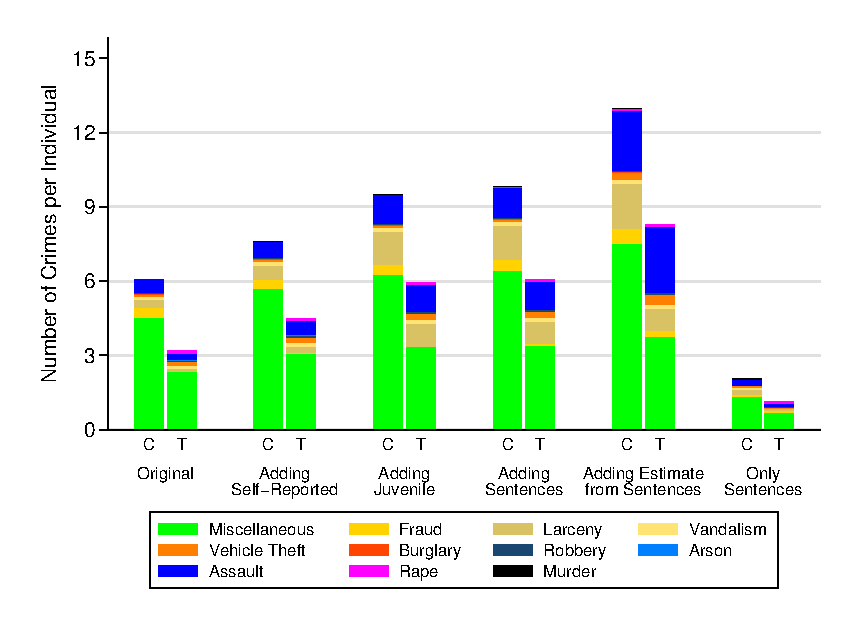
\includegraphics[width=0.8\textwidth]{AppOutput/Crime/counts_misc}
\end{center}
\end{figure}

\end{frame}

{\flushleft \normalsize Note: This chart shows the arrests per capita for the control (C) and treatment (T) groups. The first pair of bars shows the original arrests data from the administrative adult dataset. The next pair adds the self-reported crimes that did not match with the original arrests data. The next pair adds data from the administrative juvenile dataset that did not match with the previous datasets. The next pair adds one arrest for every sentence that did not match with the previous datasets and one arrest for every sentence that had arrest data missing. The next pair adds $n$ arrests instead of one for each sentence, where $n$ is calculated using the arrests-to-sentences ratio obtained from auxiliary datasets. The final pair of bars, for reference, is the total number of sentences from the administrative sentences dataset.\\}

%% ---------------------------------------------------------------------------
\begin{frame}

\begin{figure}[H]
\caption{Constructed Predictions}\label{fig:predictions}
\begin{center}
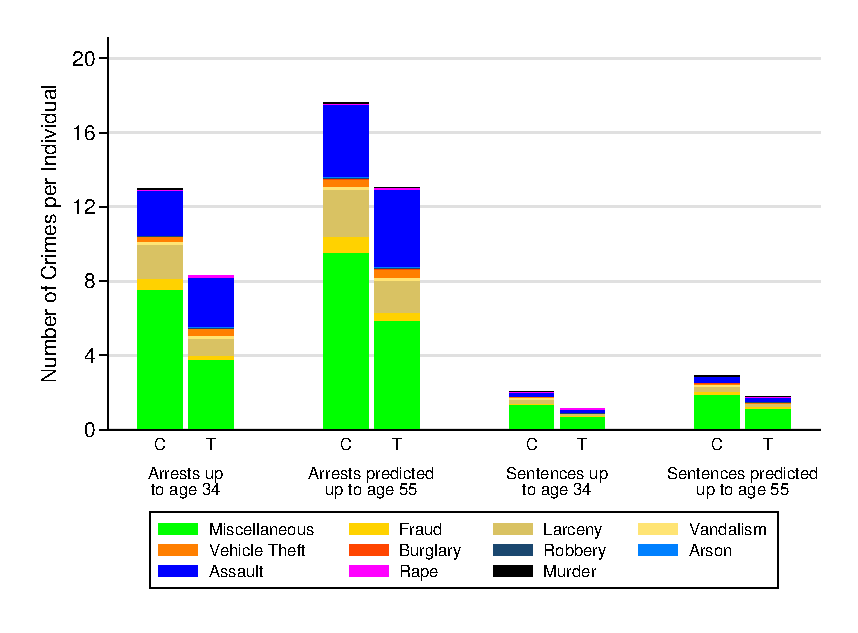
\includegraphics[width=0.8\textwidth]{AppOutput/Crime/predictions}
\end{center}
\end{figure}

\end{frame}

{\flushleft \normalsize Note: This figure continues Figure \ref{fig:datagraph}. It shows, for the control (C) and treatment (T) groups, the effects of adding predictions. The first pair of columns is the same as the fifth pair of columns in Figure \ref{fig:datagraph}. The second pair of columns includes the arrests that we predict. The third and fourth pairs of columns are the analogous pairs for sentences.\\}

\clearpage
%% ---------------------------------------------------------------------------
\begin{frame}

\begin{center}
\textbf{Victimization Inflation}
\end{center}

\end{frame}

%% ---------------------------------------------------------------------------
\begin{frame}

\begin{itemize}
\item Even though we have administrative data on crimes, we only observe the crimes that had justice system consequences (arrests or sentences).
\item However, it is possible that the subjects committed more crimes than what we observe.
\item Victimization Inflation (VI) is a method to capture benefits in crime reduction for crimes that did not result in justice system consequences.
\item For most types of crimes in the U.S., there are many more victims than arrests or sentences.
\item Using arrests as an example, VI assumes that those ``unpunished crimes'' were committed by the same people who were arrested for crimes of the same type, and in the same proportion.
\item The calculation of VI uses as an input the national ratios of total number of reported crimes over the number of arrests.
\end{itemize}

\end{frame}

%% ---------------------------------------------------------------------------
\begin{frame}

\begin{itemize}
\item VI assumes that those national ratios are also valid for each individual.
\item Under those assumptions, it is possible to find the total number of crimes committed by a subject for a given type of crime as the total number of arrests for that type of crime multiplied by the estimated national ratios for that type of crime.
\item We estimate the total number of victims using two methods, one based on arrests and one based on sentences.
\item Given that the ``unpunished'' crimes are by definition unobserved, it is not straightforward to use a data-driven method to allocate them between those subjects with arrests, those with sentences, and those with neither arrests nor sentences.
\item We calculate separate estimates for arrests and sentences and use the average of those estimates as our main estimate.
\end{itemize}

\end{frame}

%% ---------------------------------------------------------------------------
\begin{frame}

\begin{figure} [H]
\caption{Victims-to-Arrests Ratios by Crime}\label{fig:victim1}
\begin{center}
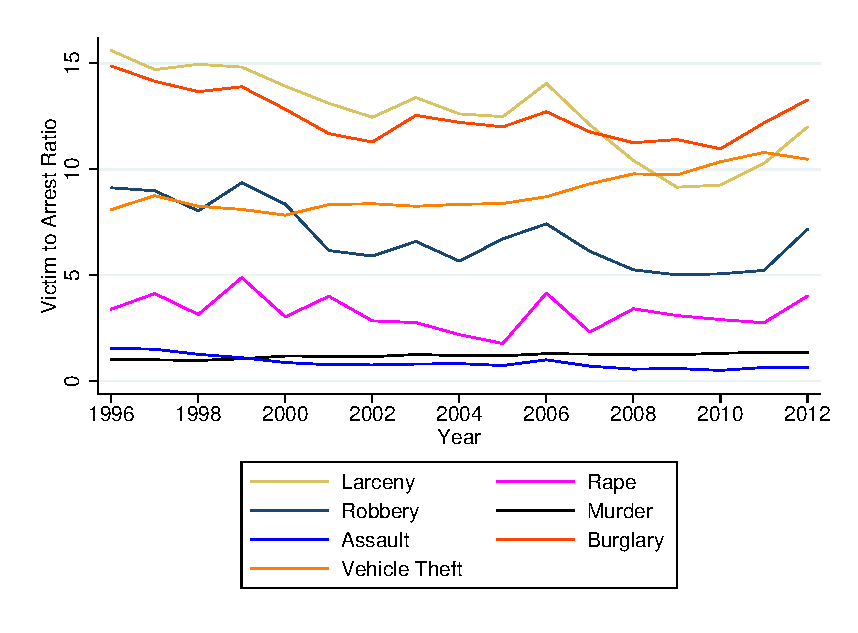
\includegraphics[width=0.8\textwidth]{AppOutput/Crime/v-to-a-ratios}
\end{center}
\end{figure}

\end{frame}

{\flushleft \normalsize Note: This figure shows, by year and type of crime, the number of victims (estimated from the NCVS and the UCRS datasets) divided by the number of arrests (estimated from the National Arrests Analysis Tool from the NBJS). In practice, we use a single number for each type of crime, which is an average across years.\\}

%% ---------------------------------------------------------------------------
\begin{frame}

\begin{figure} [H]
\caption{Arrests-to-Sentences Ratio by Crime}\label{fig:victim2}
\begin{center}
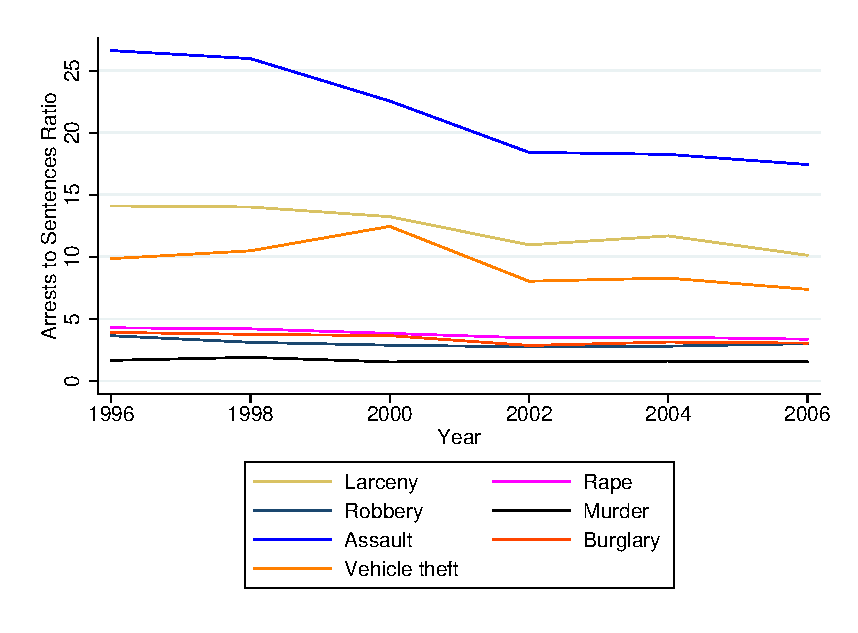
\includegraphics[width=0.8\textwidth]{AppOutput/Crime/a-to-s-ratios}
\end{center}
\end{figure}

\end{frame}

{\flushleft \normalsize Note: This figure shows, by year and type of crime, the number of arrests (estimated from the National Arrests Analysis Tool from the NBJS) divided by the number of sentences (estimated from the National Justice Reporting Program). In practice, we use a single number for each type of crime, which is an average across years.\\}

%% ---------------------------------------------------------------------------
\begin{frame}

\begin{center}
\textbf{Effects on Number of Crimes, After Victimization Inflation}
\end{center}
\begin{itemize}
\item Figure \ref{fig:count-vi} shows the effects of VI on our estimates of the number of crimes committed.
\item Note that the magnitudes in the axis are much larger than those of previous charts.
\item The largest effects are for larceny, which is common in the data and has a victims-to-arrests factor of 12.6, the largest factor of all the categories of crime used in the paper.
\item Given that the victim cost of larcenies is low, it affects the estimates less than what this chart suggests.
\end{itemize}

\end{frame}

%% ---------------------------------------------------------------------------
\begin{frame}

\begin{figure}[H]
\caption{Effects on Number of Crimes, After Victimization Inflation}\label{fig:count-vi}
\begin{center}
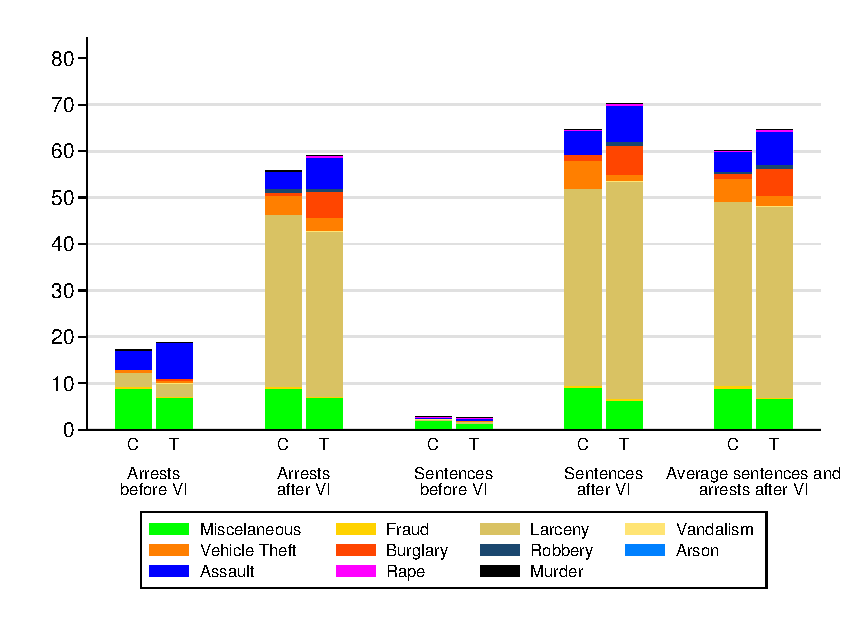
\includegraphics[width=0.8\textwidth]{AppOutput/Crime/vi}
\end{center}
\end{figure}

\end{frame}

{\flushleft \normalsize Note: This chart continues Figure \ref{fig:predictions}. It shows, for the control (C) and treatment (T) groups, the effects of adding victimization inflation (VI). The first pair of columns is the same as the second pair of columns in Figure \ref{fig:predictions}. The second pair of columns expand the arrests to account for VI. The third pair of columns is the same as the fourth pair of columns in Figure \ref{fig:predictions}. The fourth pair of columns expand the sentences to account for VI. The last pair of columns averages the second and the fourth pairs of columns in this chart.\\}

%% ---------------------------------------------------------------------------
\begin{frame}

\begin{center}
\textbf{Classifying the Costs of Crime}
\end{center}
Some methodologies used to estimate costs of crime are only able to capture some types of costs, and it might not even be clear what other methodologies are capturing. Some important types of costs are:
\begin{itemize}
\item Costs to the victim that can be directly quantified, such as medical bills, property losses, and lost productivity.
\item Costs to the victim that cannot be observed, such as pain and suffering.
\item Costs to the community in terms of prevention of crime, such as alarms, avoidance behavior, and police presence.
\item Costs to the community in terms of fear.
\item Costs to the community in terms of the criminal justice system, especially imprisonment.
\item Costs to the offender in terms of lowered productivity, such as forgone wages.
\end{itemize}

\end{frame}

%% ---------------------------------------------------------------------------
\begin{frame}

\begin{center}
\textbf{Bottom-up (BU) Methodologies}
\end{center}
\mode<presentation>{\begin{footnotesize}}
\begin{itemize}
\item These approaches sum each type of cost that is imposed after the crime has been committed.
\item The most well-known studies combine direct (also known as tangible) costs of the crimes with intangible costs.
\item Tangible costs are everything that can be directly measured by observation, such as foregone wages, hospital costs, and police expenditure.
\item Intangible costs are subjective, like pain and suffering.
\item One way to measure these costs is using jury awards.
\item For example, a jury award given as a result of an arm broken at a construction site can be used as a proxy of the intangible cost of having an arm broken in an assault.
\item The problem of these approaches is that many of the costs of crime are not directly imposed on the victim and are hard to quantify, such as the ``fear of crime,'' the increased expenditure on crime prevention, and the negative impact of imprisonment on the community.
\end{itemize}
\mode<presentation>{\end{footnotesize}}

\end{frame}

%% ---------------------------------------------------------------------------
\begin{frame}

\begin{center}
\textbf{Top-down (TD) Methodologies}
\end{center}
\begin{itemize}
\item The other way to estimate the cost of crime is using TD methods, based on eliciting willingness to pay for avoiding crimes.
\item The main advantage of these methods is that, in principle, they consider costs that are hard or impossible to measure directly, such as the cost of fear, avoidance behavior, and expenditures in preventative measures.
\item There are three main methodologies for this approach, which we now briefly describe.
\end{itemize}

\end{frame}

%% ---------------------------------------------------------------------------
\begin{frame}

\begin{enumerate}
\item Stated Preferences
    \begin{itemize}
    \item This basic method elicits the willingness to pay for hypothetical programs that would reduce crime nationwide for a sample of people.
    \item Being an example of a TD methodology, it is expected that the costs obtained by this method would include factors that affect the community, and that are hard to capture, such as fear.
    \item However, it is unclear whether people consider factors like the cost of the justice system in their answers to these questions.
    \item An obvious caveat of this method is that people might not answer the real amount they would be willing to pay in these surveys.
    \end{itemize}
\end{enumerate}

\end{frame}

%% ---------------------------------------------------------------------------
\begin{frame}

\begin{enumerate}
\setcounter{enumi}{1}
\item Revealed Preferences
    \begin{itemize}
    \item This method infers the value that individuals assign to crime reductions from market transactions.
    \item The most standard way to calculate these estimations is running regressions to explain the total price of houses with several factors, including the rates of crime in the area.
    \item Those parameters associated with the crime rate are considered the revealed valuation of avoiding crimes.
    \item One weakness of this method is that it assumes that people are well-informed on the crime rates in an area.
    \item Another problem is that, in absence of extremely large and rich data on crimes and housing prices, it is not possible to separately identify the costs of different types of crimes.
    \item To the best of our knowledge, no paper has yet been able to convincingly obtain estimates per type of crime with this method.
    \end{itemize}
\end{enumerate}

\end{frame}

%% ---------------------------------------------------------------------------
\begin{frame}

\begin{enumerate}
\setcounter{enumi}{2}
\item Life Satisfaction
    \begin{itemize}
    \item For this method, people are surveyed about their preferences between different life conditions, in which several different factors are considered.
    \item Some of those factors are income and rates of crime.
    \item By doing so, people implicitly associate monetary values to the levels of crime in the communities they would live in.
    \end{itemize}
\end{enumerate}

\end{frame}

%% ---------------------------------------------------------------------------
\begin{frame}

\begin{center}
\textbf{Costs Used in This Study}
\end{center}
\begin{itemize}
\item To summarize, both approaches have strengths and weaknesses: the TD approaches are more likely to reflect costs to the community (e.g. fear and anxiety, avoidance behavior, and protective measures) and better capture the spirit of a prevention program.
\item However, in practice TD estimates rely on strong assumptions, and there are methodological issues associated with obtaining detailed values for the different types of crimes.
\item It is also possible that when people answer the survey used for TD calculations they include some costs that we are including separately, such as justice system costs, and risk of death from non-murder crimes, while BU does not include them.
\end{itemize}

\end{frame}

%% ---------------------------------------------------------------------------
\begin{frame}

\begin{center}
\textbf{Costs Used in This Study}
\end{center}
\begin{itemize}
\item Given those considerations, and the lack of TD costs for some categories of crime, we use BU costs for our main estimates.
\item For completeness, we present cost estimates using both approaches.
\item We choose \cite{Cohen_Rust_etal_2004_Criminology} as representative of the TD approaches, and \cite{McCollister_etal_2010_DAD} as representative of the BU approaches.
\item In terms of timing, both of these studies match well with the ABC and CARE data.
\end{itemize}

\end{frame}

%% ---------------------------------------------------------------------------
\begin{frame}

\begin{center}
\textbf{Costs Used in This Study}
\end{center}
\begin{itemize}
\item The bulk of crimes in the ABC and CARE data occurred between the late 1990s and early 2000s.
\item While \cite{Cohen_Rust_etal_2004_Criminology} do not report the exact year of their survey, they use Census 2000 figures for their estimates.
\item Even though \cite{McCollister_etal_2010_DAD} is a more recent study, many of the productivity estimates that their costs are based on are taken from papers using data from years with more crimes the late 1990s and early 2000s.
\item The costs in those studies are presented in Table \ref{tab:individual-crime-cost}.
\item Notice that there are some strong differences in the cost of crimes, such as assault, burglary, and especially robbery.
\end{itemize}

\end{frame}

%% ---------------------------------------------------------------------------
\begin{frame}

\begin{table}[H]
\caption{Monetary Costs of Crime for Victims} \label{tab:individual-crime-cost}
\begin{center}
\mode<presentation>{\begin{small}}
\begin{tabular}{lcc}
\toprule
Crime				&Top-Down Approach	&Bottom-Up Approach	\\
					& \cite{Cohen_Rust_etal_2004_Criminology}&\cite{McCollister_etal_2010_DAD}\\ \midrule
Arson				&					&12,093			\\
Assault				&95,200			&16,132 			\\
Burglary			&34,000			&1,467 			\\		
Fraud				&				&0				\\
Larceny				&				&528 				\\
Motor Vehicle Theft	&				&6,699 			\\
Murder				&13,192,000		&9,286,200 		\\
Rape				&322,320			&224,021 			\\
Robbery				&315,520			&7,273 			\\
Vandalism			&					&0				\\ \bottomrule
\end{tabular}
\mode<presentation>{\end{small}}
\end{center}
\end{table}

\end{frame}

{\flushleft \normalsize Note: All amounts are in 2014 USD. The amounts reported in \cite{McCollister_etal_2010_DAD} for non-murder crimes have the extra cost for risk of death and the cost of a crime career removed (both were obtained from correspondence with the author). Risk-of-death costs do not apply, because we know the outcomes of the crimes. Crime-career costs do not apply, as we directly observe the income of the individuals. These costs also don't include police and legal system costs, as those are imputed separately and only for the cases for which individuals were arrested or sentenced.\\}

%% ---------------------------------------------------------------------------
\begin{frame}

\begin{figure} [H]
\caption{Costs of Crime Before Victimization Inflation}\label{tab:diff-costs}
\begin{center}
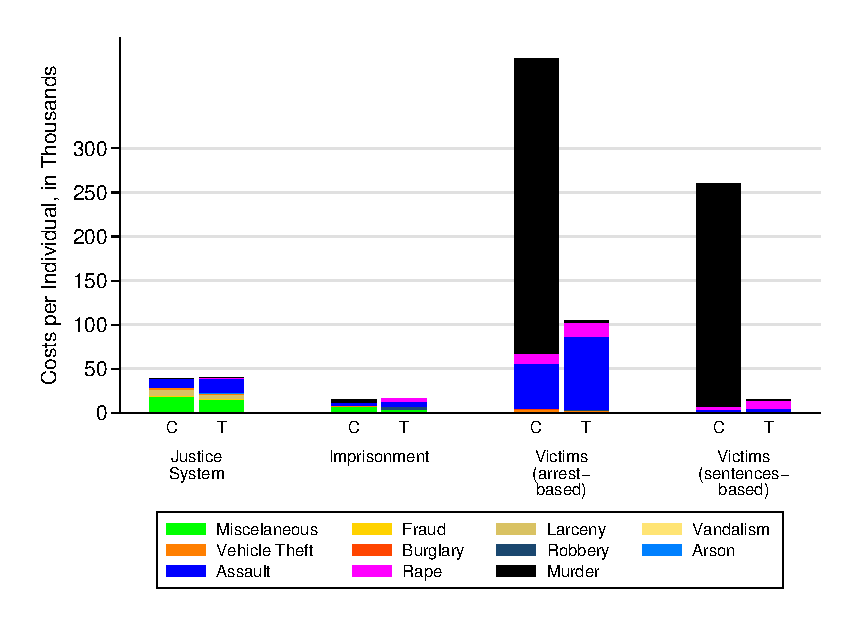
\includegraphics[width=0.8\textwidth]{AppOutput/Crime/different_costs}
\end{center}
\end{figure}

\end{frame}

{\flushleft \normalsize Note: This figure depicts the per capita cost for the different categories of costs and crimes we use, by control (C) and treatment (T). The first pair of columns adds up the justice system costs (including police) for all arrests inputed for each subject. The second pair of columns adds up the cost of Imprisonment. It is important to note that the costs are per capita, so there are individual cases that have much higher costs. The next two pairs of columns show the pre-victimization inflation estimates of number of crimes multiplied by the individual victim cost of the different crimes. The costs are taken from the Bottom-up approach in Table \ref{tab:individual-crime-cost}. All costs are in thousands of 2014 USD.\\}

%% ---------------------------------------------------------------------------
\begin{frame}

\begin{figure} [H]
\caption{Costs of Crime After Victimization Inflation}\label{tab:costs_vi}
\begin{center}
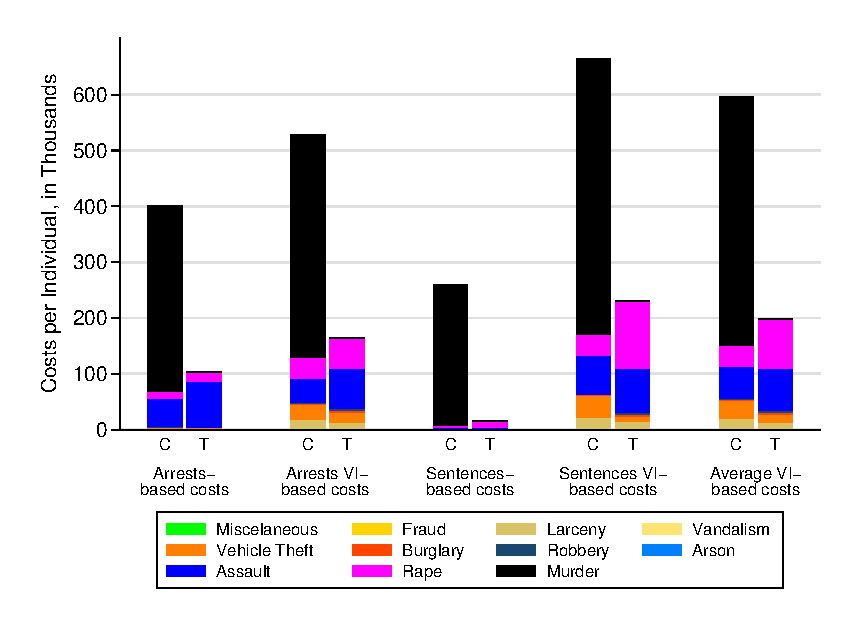
\includegraphics[width=0.8\textwidth]{AppOutput/Crime/costs_vi}
\end{center}
\end{figure}

\end{frame}

{\flushleft \normalsize Note: This figure depicts the per capita cost for the different categories of costs and crimes we use, by control (C) and treatment (T). The first two pairs of columns adds up all of the arrest-based costs for each subject and compares the pre- and post-victimization inflation costs. The third and fourth pair of columns compare the pre- and post-victimization inflation sentence-based costs. It is important to note that the costs are per capita, so there are individual cases that have much higher costs. The next two pairs of columns show the post-victimization inflation estimates of number of crimes multiplied by the individual victim cost of the different crimes. The costs are taken from the Bottom-up approach in Table \ref{tab:individual-crime-cost}. All costs are in thousands of 2014 USD.\\}

%% ---------------------------------------------------------------------------
\begin{frame}

\begin{center}
\hyperlink{ret:muffin}{\underline{Return to main text}}
\end{center}

\end{frame}

%% ---------------------------------------------------------------------------
{\mode<presentation>{\section[Details]{Program Details}}}
%-----------------------------------------------------------------------------
\begin{frame}

\hypertarget{scrambledeggs}{}
\begin{center}
\textbf{Program Details}
\end{center}

\end{frame}

%% ---------------------------------------------------------------------------
\begin{frame}\label{secondphase}
\frametitle{First-phase Treatment, ABC}

\begin{itemize}
\item First-phase Treatment, ABC: one control group and one treatment group
	\begin{itemize}
	\item Control group (56 children):
		\begin{enumerate}								
		\item Iron-fortified formula and monthly supply of diapers, first 15 months of life
		\end{enumerate}
	\item Treatment group (58 children):
		\begin{enumerate}
		\item Iron-fortified formula and monthly supply of diapers, first 15 months of life
		\item Breakfast, lunch, and afternoon snack
		\item Medical care from nurses, supervised by a doctor
		\item Center-based childcare
		\end{enumerate}
	\end{itemize}			
\end{itemize}

\end{frame}

%% ---------------------------------------------------------------------------
\begin{frame}
\frametitle{First-phase Treatment, CARE}

\begin{itemize}
\item First-phase Treatment, CARE: one control group and two treatment groups
	\begin{itemize}
	\item Control group (23 children):
		\begin{enumerate}								
		\item Iron-fortified formula and monthly supply of diapers, first 15 months of life
		\end{enumerate}
	\item Family education treatment group (27 children)
		\begin{enumerate}
		\item Iron-fortified formula and monthly supply of diapers, first 15 months of life
		\item Home visits that aimed to help parents solve common problems related to child rearing.
		\end{enumerate}
	\item Center-based childcare and family education treatment group (16 children):
		\begin{enumerate}
		\item Same as the family education treatment group
		\item Center-based childcare	
		\end{enumerate}							
    \end{itemize}
\end{itemize}

\end{frame}

%% ---------------------------------------------------------------------------
\begin{frame}
\frametitle{Second-phase Treatment, ABC and CARE}

\begin{itemize}
\item For both programs: home visits from ages 5 to 8 \\
	$\rightarrow$ similar in objectives to first-phase home visits of CARE
\item ABC: re-randomized at age 5 to either receive or not the home visits \\
	$\rightarrow$ 96 children were re-randomized
\item CARE: participants of the two first-phase treatment groups received second-phase treatment
\end{itemize}

\end{frame}

\textbf{[JJH: Where do we show that home visiting has no effect 5--8 for both boys and girls?] [JLG: we documented this. Please recall only ABC had second-phase randomization. The document is being printed for you today]}
\clearpage
%% ---------------------------------------------------------------------------
\begin{frame}
\frametitle{Eligibility}

\begin{itemize}
\item Both programs targeted disadvantaged children from the semi-rural communities of Chapel Hill close to the Frank Porter Graham Center (FPGC) of the University of North Carolina
	\begin{itemize}
	\item Mothers in the last trimester of pregnancy were referred by local social service agencies and hospitals 		
	\item Eligibility was determined by a score of 11 or more on the High-risk Index (HRI)
	\item Example HRI items:
		\begin{itemize}
		\item Mother's education level
		\item Use of welfare programs
		\item Father's presence at home
		\end{itemize}
    \item Although race was not a consideration for eligibility, 98\% of ABC participants and 90\% of CARE participants were African-American
	\end{itemize}
\end{itemize}

\end{frame}

\textbf{[JJH: Can we get full components of HRI? People do not just want examples.] [JLG: this is the exact way in which the HRI is computed. Note that this is already listed in Appendix A and distributions of the HRI are plotted per your previous request.\\
The HRI for ABC was based on 13 weighted variables, which are listed here with weights in parentheses: (i) maternal education level measured by years of education- 6 (8), 7 (7), 8 (6), 9 (3), 10 (2), 11 (1), 12 (0); (ii) paternal education level with weights identical to those for maternal education; (iii) yearly family income measured in current dollars -- \$1,000 or less (8), \$1,001--\$2000 (7), \$2,001--\$3,000 (6), \$3,001--\$4,000 (5), \$4,001--\$5,000 (4), \$5,001--\$6,000 (0); (iv) father's absence from the household for reasons other than health or death (3); (v) lack of maternal relatives in the area (3); (vi) siblings of school age one or more grades behind age-appropriate level, or with equivalently low scores on school-administered achievement tests (3); (vii) received payments from welfare agencies within the past 3 years (3); (viii) record of father's work indicates instability or unskilled and semi-skilled labor (3); (ix) record of maternal or paternal IQ score of 90 or below (3); (x) record of a sibling with an IQ score of 90 or below (3); (xi) relevant social agencies in the community indicate the family is in need of assistance (3); (xii) one or more family members has sought counseling or professional help in the past 3 years (1); and (xiii) special circumstances not included in any of the above that are likely contributors to cultural or social disadvantage (1). The weighting scale aimed to establish the relative importance of each item in the index. Race was not considered for eligibility; however, 98\% of the families who agreed to participate were African-American.]}

\clearpage
%% ---------------------------------------------------------------------------
\begin{frame}
\frametitle{Sample}\label{sample}

\begin{itemize}
\item ABC
	\begin{itemize}
	\item Four cohorts of children born between 1972 and 1977
	\item 122 individuals recruited
	\end{itemize}
\item CARE
	\begin{itemize}
	\item Two cohorts of children born in 1978 and 1979
	\item 67 individuals recruited
	\end{itemize}
\item Overall, mothers in CARE were older, more educated, and had higher IQ than the mothers in ABC
\end{itemize}

\end{frame}

%% ---------------------------------------------------------------------------
\begin{frame}
\frametitle{ABC and CARE Samples in Context}

\begin{itemize}
\item We compare the ABC and CARE samples to a comparison group using a cohort of the Panel Study of Income Dynamics born in the same years as the ABC and CARE subjects (1972-1979)
\item ABC and CARE subjects were born to younger, less educated mothers many of whom were raising their children without the father present
\end{itemize}

\end{frame}

%% ---------------------------------------------------------------------------
\begin{frame}
\frametitle{ABC Randomization}

\begin{itemize}
\item First Phase: 121 children randomized to one treatment group that received center-based childcare and one control group
	\begin{itemize}
	\item Effective sample size after randomization compromises: 114 (58 treatment, 56 control)
	\end{itemize}
\item Second Phase: 96 of the original children were randomized into one treatment and one control group
\end{itemize}

\end{frame}

%% ---------------------------------------------------------------------------
\begin{frame}
\frametitle{CARE Randomization}

\begin{itemize}
\item First Phase: 67 children randomized into:
	\begin{itemize}
	\item One treatment group that received center-based childcare and family education (16 children)
	\item One treatment group that only received family education (27 children)
	\item One control group (23 children)
	\end{itemize}
\item Second Phase: Children in the two treatment groups automatically received the second-phase treatment of home visits and the control group remained the same
\item No randomization compromises except death and families moving away from the study area
\end{itemize}

\end{frame}

%% ---------------------------------------------------------------------------
\begin{frame}
\frametitle{ABC First-phase Randomization Compromises}

\begin{enumerate}
\item \textbf{Left the study before data collection:} We have no data at all for these subjects (4 treatment)
\item \textbf{Death before age 5 / Moved out:} We include them in estimations until data are no longer available. Thereafter, they are cases of attrition (2 treatment and 2 control)
\item \textbf{Partial treatment:} We assume that they had full treatment (4 children)
\item \textbf{Noncompliance to treatment:} We keep the original treatment status for them for ITT estimations (3 treatment)
\item \textbf{Crossover from control to treatment:} Three children switched status from control to treatment. We keep the original treatment statuses for ITT estimations (3 children)
\item \textbf{Developmental delays:} We drop them because they were not eligible for the program (2 treatment)
\end{enumerate}

\end{frame}

%% ---------------------------------------------------------------------------
\begin{frame}
\frametitle{ABC Second-phase Randomization Compromises}

\begin{enumerate}
\item \textbf{Not randomized in second phase:}
	\begin{itemize}
	\item \underline{Stopped being followed-up:} They are considered cases of attrition
    \item \underline{Followed-up in later data collection:} They are not included when calculating the treatment effects for the second phase, but are included when estimating treatment effects of the first phase on later outcomes
	\end{itemize}
\item \textbf{Noncompliance in second phase:} Original treatment statuses are kept for ITT estimations
\end{enumerate}

\end{frame}

\clearpage
%% ---------------------------------------------------------------------------
\begin{frame}
\frametitle{Programmatic Elements}

\begin{itemize}
\item The objectives of both ABC and CARE were to prevent ``mental retardation'' and develop school readiness
\item The different curricula implemented across the programs and cohorts had the following goals:
	\begin{itemize}
    \item Support language and cognitive development
	\item Develop socio-emotional skills considered to enable school-readiness (e.g., task orientation)
	\end{itemize}
\end{itemize}

\end{frame}

%% ---------------------------------------------------------------------------
\begin{frame}
\frametitle{Additional Programmatic Elements}

\begin{itemize}
\item The ABC treatment group received
	\begin{itemize}
	\item Daily health screenings and frequent medical check-ups
	\end{itemize}
\item The CARE treatment groups received
	\begin{itemize}
	\item Home visits to help parents form problem-solving skills
	\end{itemize}
\item Both ABC and CARE center-based treatment groups received
	\begin{itemize}
	\item Transportation to and from FPGC
	\item Daily nutritious food
	\end{itemize}
\item Both ABC and CARE control groups received
	\begin{itemize}
	\item Iron-fortified formula until the child was 15 months old
	\item Unlimited diapers until the child was 3 years old
	\end{itemize}
\end{itemize}

\end{frame}

\textbf{[JJH: Any medical check-ups?] [JLG: zero evidence on that.]}
\clearpage
%% ---------------------------------------------------------------------------
\begin{frame}
\frametitle{Programmatic Elements, Second Phase}\label{elements}

\begin{itemize}	
\item Same treatment in ABC and CARE
\item State-certified ``home-school resource teachers"
\item Visited the elementary school and the children's homes twice a month to help
	\begin{itemize}
	\item Engage the parents with the children's academics
	\item Provide one-on-one tutoring to the children
	\item Parents with issues related to literacy, housing, and medical care
	\end{itemize}
\end{itemize}

\end{frame}

%% ---------------------------------------------------------------------------
\begin{frame}
\frametitle{Baseline Characteristics in ABC and CARE}\label{baseline_abccare}

\begin{table}[H]
\caption{Baseline Characteristics in ABC and CARE}
\begin{center}
\mode<presentation>{\scalebox{0.75}{\begin{table}[H]
\captionsetup{singlelinecheck=false,justification=centering}
\caption{Baseline Characteristics Comparison between ABC and CARE \label{tab:baseline}}

  \begin{threeparttable}
  \begin{tabular}{cccccccc} \toprule

     &  & \scriptsize{ABC} & \scriptsize{CARE} & \scriptsize{ABC} & \scriptsize{CARE} & \mc{2}{c}{\scriptsize{$p$-value}} \\  

    \scriptsize{Variable} & \scriptsize{Age} & \scriptsize{Obs} & \scriptsize{Obs} & \scriptsize{Mean} & \scriptsize{Mean} & \scriptsize{Single $H_0$} & \scriptsize{Multiple $H_0$} \\ 
    \hline  

    \mc{1}{l}{\scriptsize{Male}} & \mc{1}{c}{\scriptsize{0}} & \mc{1}{c}{\scriptsize{116}} & \mc{1}{c}{\scriptsize{67}} & \mc{1}{c}{\scriptsize{0.464}} & \mc{1}{c}{\scriptsize{0.596}} & \mc{1}{c}{\scriptsize{\textbf{(0.060)}}} & \mc{1}{c}{\scriptsize{(0.110)}} \\  

    \mc{1}{l}{\scriptsize{Birth Weight}} & \mc{1}{c}{\scriptsize{0}} & \mc{1}{c}{\scriptsize{114}} & \mc{1}{c}{\scriptsize{64}} & \mc{1}{c}{\scriptsize{7.008}} & \mc{1}{c}{\scriptsize{7.139}} & \mc{1}{c}{\scriptsize{(0.625)}} & \mc{1}{c}{\scriptsize{(0.765)}} \\  

    \mc{1}{l}{\scriptsize{No. Siblings in Household}} & \mc{1}{c}{\scriptsize{0}} & \mc{1}{c}{\scriptsize{116}} & \mc{1}{c}{\scriptsize{67}} & \mc{1}{c}{\scriptsize{0.632}} & \mc{1}{c}{\scriptsize{0.684}} & \mc{1}{c}{\scriptsize{(0.810)}} & \mc{1}{c}{\scriptsize{(0.890)}} \\  

    \mc{1}{l}{\scriptsize{Birth Year}} & \mc{1}{c}{\scriptsize{0}} & \mc{1}{c}{\scriptsize{116}} & \mc{1}{c}{\scriptsize{67}} & \mc{1}{c}{\scriptsize{1974}} & \mc{1}{c}{\scriptsize{1979}} & \mc{1}{c}{\scriptsize{\textbf{(0.000)}}} & \mc{1}{c}{\scriptsize{\textbf{(0.000)}}} \\ 
    \midrule

    \mc{1}{l}{\scriptsize{Mother's Education}} & \mc{1}{c}{\scriptsize{0}} & \mc{1}{c}{\scriptsize{116}} & \mc{1}{c}{\scriptsize{67}} & \mc{1}{c}{\scriptsize{10.188}} & \mc{1}{c}{\scriptsize{10.868}} & \mc{1}{c}{\scriptsize{\textbf{(0.010)}}} & \mc{1}{c}{\scriptsize{\textbf{(0.025)}}} \\  

    \mc{1}{l}{\scriptsize{Mother's Age}} & \mc{1}{c}{\scriptsize{0}} & \mc{1}{c}{\scriptsize{116}} & \mc{1}{c}{\scriptsize{67}} & \mc{1}{c}{\scriptsize{19.828}} & \mc{1}{c}{\scriptsize{21.141}} & \mc{1}{c}{\scriptsize{\textbf{(0.060)}}} & \mc{1}{c}{\scriptsize{\textbf{(0.100)}}} \\  

    \mc{1}{l}{\scriptsize{Mother's IQ}} & \mc{1}{c}{\scriptsize{0}} & \mc{1}{c}{\scriptsize{116}} & \mc{1}{c}{\scriptsize{67}} & \mc{1}{c}{\scriptsize{84.407}} & \mc{1}{c}{\scriptsize{87.164}} & \mc{1}{c}{\scriptsize{\textbf{(0.070)}}} & \mc{1}{c}{\scriptsize{(0.130)}} \\  

    \mc{1}{l}{\scriptsize{Father at Home}} & \mc{1}{c}{\scriptsize{0}} & \mc{1}{c}{\scriptsize{116}} & \mc{1}{c}{\scriptsize{67}} & \mc{1}{c}{\scriptsize{0.283}} & \mc{1}{c}{\scriptsize{0.209}} & \mc{1}{c}{\scriptsize{(0.270)}} & \mc{1}{c}{\scriptsize{(0.380)}} \\  

  \bottomrule
  \end{tabular}
    \begin{tablenotes}
    \scriptsize
    \item 
    Note: This table compares baseline, observed characteristics between ABC and CARE. 
    For each characteristic, we present the $p$-value from a single hypothesis test.
    We also present the $p$-values from multiple testing, where we collectively test the
    baseline characteristics within the blocks separated by the horizontal line.
    Both $p$-values are two-sided and non-parametric. We construct them 
    based on 1,000 re-draws of the full sample. The estimates we display are the means of 
    the empirical bootstrap distribution. 
    
    \end{tablenotes}
  \end{threeparttable}

\end{table}}}
\mode<article>{\begin{table}[H]
\captionsetup{singlelinecheck=false,justification=centering}
\caption{Baseline Characteristics Comparison between ABC and CARE \label{tab:baseline}}

  \begin{threeparttable}
  \begin{tabular}{cccccccc} \toprule

     &  & \scriptsize{ABC} & \scriptsize{CARE} & \scriptsize{ABC} & \scriptsize{CARE} & \mc{2}{c}{\scriptsize{$p$-value}} \\  

    \scriptsize{Variable} & \scriptsize{Age} & \scriptsize{Obs} & \scriptsize{Obs} & \scriptsize{Mean} & \scriptsize{Mean} & \scriptsize{Single $H_0$} & \scriptsize{Multiple $H_0$} \\ 
    \hline  

    \mc{1}{l}{\scriptsize{Male}} & \mc{1}{c}{\scriptsize{0}} & \mc{1}{c}{\scriptsize{116}} & \mc{1}{c}{\scriptsize{67}} & \mc{1}{c}{\scriptsize{0.464}} & \mc{1}{c}{\scriptsize{0.596}} & \mc{1}{c}{\scriptsize{\textbf{(0.060)}}} & \mc{1}{c}{\scriptsize{(0.110)}} \\  

    \mc{1}{l}{\scriptsize{Birth Weight}} & \mc{1}{c}{\scriptsize{0}} & \mc{1}{c}{\scriptsize{114}} & \mc{1}{c}{\scriptsize{64}} & \mc{1}{c}{\scriptsize{7.008}} & \mc{1}{c}{\scriptsize{7.139}} & \mc{1}{c}{\scriptsize{(0.625)}} & \mc{1}{c}{\scriptsize{(0.765)}} \\  

    \mc{1}{l}{\scriptsize{No. Siblings in Household}} & \mc{1}{c}{\scriptsize{0}} & \mc{1}{c}{\scriptsize{116}} & \mc{1}{c}{\scriptsize{67}} & \mc{1}{c}{\scriptsize{0.632}} & \mc{1}{c}{\scriptsize{0.684}} & \mc{1}{c}{\scriptsize{(0.810)}} & \mc{1}{c}{\scriptsize{(0.890)}} \\  

    \mc{1}{l}{\scriptsize{Birth Year}} & \mc{1}{c}{\scriptsize{0}} & \mc{1}{c}{\scriptsize{116}} & \mc{1}{c}{\scriptsize{67}} & \mc{1}{c}{\scriptsize{1974}} & \mc{1}{c}{\scriptsize{1979}} & \mc{1}{c}{\scriptsize{\textbf{(0.000)}}} & \mc{1}{c}{\scriptsize{\textbf{(0.000)}}} \\ 
    \midrule

    \mc{1}{l}{\scriptsize{Mother's Education}} & \mc{1}{c}{\scriptsize{0}} & \mc{1}{c}{\scriptsize{116}} & \mc{1}{c}{\scriptsize{67}} & \mc{1}{c}{\scriptsize{10.188}} & \mc{1}{c}{\scriptsize{10.868}} & \mc{1}{c}{\scriptsize{\textbf{(0.010)}}} & \mc{1}{c}{\scriptsize{\textbf{(0.025)}}} \\  

    \mc{1}{l}{\scriptsize{Mother's Age}} & \mc{1}{c}{\scriptsize{0}} & \mc{1}{c}{\scriptsize{116}} & \mc{1}{c}{\scriptsize{67}} & \mc{1}{c}{\scriptsize{19.828}} & \mc{1}{c}{\scriptsize{21.141}} & \mc{1}{c}{\scriptsize{\textbf{(0.060)}}} & \mc{1}{c}{\scriptsize{\textbf{(0.100)}}} \\  

    \mc{1}{l}{\scriptsize{Mother's IQ}} & \mc{1}{c}{\scriptsize{0}} & \mc{1}{c}{\scriptsize{116}} & \mc{1}{c}{\scriptsize{67}} & \mc{1}{c}{\scriptsize{84.407}} & \mc{1}{c}{\scriptsize{87.164}} & \mc{1}{c}{\scriptsize{\textbf{(0.070)}}} & \mc{1}{c}{\scriptsize{(0.130)}} \\  

    \mc{1}{l}{\scriptsize{Father at Home}} & \mc{1}{c}{\scriptsize{0}} & \mc{1}{c}{\scriptsize{116}} & \mc{1}{c}{\scriptsize{67}} & \mc{1}{c}{\scriptsize{0.283}} & \mc{1}{c}{\scriptsize{0.209}} & \mc{1}{c}{\scriptsize{(0.270)}} & \mc{1}{c}{\scriptsize{(0.380)}} \\  

  \bottomrule
  \end{tabular}
    \begin{tablenotes}
    \scriptsize
    \item 
    Note: This table compares baseline, observed characteristics between ABC and CARE. 
    For each characteristic, we present the $p$-value from a single hypothesis test.
    We also present the $p$-values from multiple testing, where we collectively test the
    baseline characteristics within the blocks separated by the horizontal line.
    Both $p$-values are two-sided and non-parametric. We construct them 
    based on 1,000 re-draws of the full sample. The estimates we display are the means of 
    the empirical bootstrap distribution. 
    
    \end{tablenotes}
  \end{threeparttable}

\end{table}}
\end{center}
\end{table}

\end{frame}

%% ---------------------------------------------------------------------------
\begin{frame}
\frametitle{Programmatic Elements, First Phase Treatment}\label{first_phase}
	
\begin{table}[H]
\caption{Elements of First Phase Treatment, ABC and CARE}
\begin{center}
\mode<presentation>{\scalebox{0.55}{\begin{tabular}{L{4cm} L{7cm} L{7cm}} 
\toprule
& \multicolumn{1}{c}{ABC}& \multicolumn{1}{c}{CARE} \\
\midrule
\textbf{Treatment} & Center-based childcare & Center-based childcare and family education \\
\hspace{.5cm} \textbf{Center-based} \\
\hspace{.5cm} \textbf{Childcare} \\
\hspace{.5cm} Intensity &6.5--9.75 hours a day for 50 weeks per year& 6.5--9.75 hours a day for 50 weeks per year \\
\hspace{.5cm} Components & Instruction, medical care, nutrition, social services & Instruction, medical care, nutrition, social services \\
\hspace{.5cm} Staff-to-child Ratio &1:3 during ages 0--1 &1:3 during ages 0--1 \\
&1:4--5 during age 1--4 &1:4--5 during age 1--4 \\
&1:5--6 during ages 4--5 & 1:5--6 during ages 4--5 \\
\hspace{.5cm} Staff Qualifications &Mixed diplomas; experienced& Mixed diplomas; experienced \\ \\
\hspace{.5cm} \textbf{Family Education}  & \\
\hspace{.5cm} Intensity & & One hour-long home visits. 2--3 per month during ages 0--3. 1--2 per month during ages 4--5\\
\hspace{.5cm} Curriculum & & Social and mental stimulation; parent-child interaction\\
\hspace{.5cm} Staff-to-child Ratio & & 1:1\\
\hspace{.5cm} Staff Qualifications & & Home visitor training\\
\bottomrule
\end{tabular}}}
\mode<article>{\scalebox{0.85}{\begin{tabular}{L{4cm} L{7cm} L{7cm}} 
\toprule
& \multicolumn{1}{c}{ABC}& \multicolumn{1}{c}{CARE} \\
\midrule
\textbf{Treatment} & Center-based childcare & Center-based childcare and family education \\
\hspace{.5cm} \textbf{Center-based} \\
\hspace{.5cm} \textbf{Childcare} \\
\hspace{.5cm} Intensity &6.5--9.75 hours a day for 50 weeks per year& 6.5--9.75 hours a day for 50 weeks per year \\
\hspace{.5cm} Components & Instruction, medical care, nutrition, social services & Instruction, medical care, nutrition, social services \\
\hspace{.5cm} Staff-to-child Ratio &1:3 during ages 0--1 &1:3 during ages 0--1 \\
&1:4--5 during age 1--4 &1:4--5 during age 1--4 \\
&1:5--6 during ages 4--5 & 1:5--6 during ages 4--5 \\
\hspace{.5cm} Staff Qualifications &Mixed diplomas; experienced& Mixed diplomas; experienced \\ \\
\hspace{.5cm} \textbf{Family Education}  & \\
\hspace{.5cm} Intensity & & One hour-long home visits. 2--3 per month during ages 0--3. 1--2 per month during ages 4--5\\
\hspace{.5cm} Curriculum & & Social and mental stimulation; parent-child interaction\\
\hspace{.5cm} Staff-to-child Ratio & & 1:1\\
\hspace{.5cm} Staff Qualifications & & Home visitor training\\
\bottomrule
\end{tabular}}}
\end{center}
\end{table}

\end{frame}

%% ---------------------------------------------------------------------------
\begin{frame}
\frametitle{Programmatic Elements, Second Phase Treatment}
	
\begin{table}[H]
\caption{Elements of Second Phase Treatment, ABC and CARE}
\begin{center}
\mode<presentation>{\scalebox{0.6}{ \begin{tabular}{L{4cm} L{7cm} L{7cm}} 
\toprule
& \multicolumn{1}{c}{ABC}& \multicolumn{1}{c}{CARE}  \\ \midrule
\hspace{.5cm} Intensity &Every other week& Every other week \\
\hspace{.5cm} Components &Parent-teacher meetings& Parent-teacher meetings \\
\hspace{.5cm} Curriculum & Reading and math &  Reading and math \\
\hspace{.5cm} Staff-to-child Ratio &1:1& 1:1 \\
\hspace{.5cm} Staff Qualifications &Graduate degree and training in special education & Graduate degree and training in special education \\
\bottomrule
\end{tabular}}}
\mode<article>{\scalebox{0.8}{ \begin{tabular}{L{4cm} L{7cm} L{7cm}} 
\toprule
& \multicolumn{1}{c}{ABC}& \multicolumn{1}{c}{CARE}  \\ \midrule
\hspace{.5cm} Intensity &Every other week& Every other week \\
\hspace{.5cm} Components &Parent-teacher meetings& Parent-teacher meetings \\
\hspace{.5cm} Curriculum & Reading and math &  Reading and math \\
\hspace{.5cm} Staff-to-child Ratio &1:1& 1:1 \\
\hspace{.5cm} Staff Qualifications &Graduate degree and training in special education & Graduate degree and training in special education \\
\bottomrule
\end{tabular}}}
\end{center}
\end{table}

\end{frame}

%% ---------------------------------------------------------------------------
\begin{frame}

\begin{center}
\hyperlink{ret:scrambledeggs}{\underline{Return to main text}}
\end{center}

\end{frame}

\clearpage

%% ---------------------------------------------------------------------------
{\mode<presentation>{\section[Combining]{Estimated Combining Functions by Outcome Categories}}}
%-----------------------------------------------------------------------------
\begin{frame}

\hypertarget{estimated-comb}{}
\begin{center}
\textbf{Estimated Combining Functions by Outcome Categories}
\end{center}

\end{frame}

%% ---------------------------------------------------------------------------
\begin{frame}

\begin{figure}[H]
\caption{Percentage of Outcomes with Positive Treatment Effects, First Set of Categories}
\begin{center}
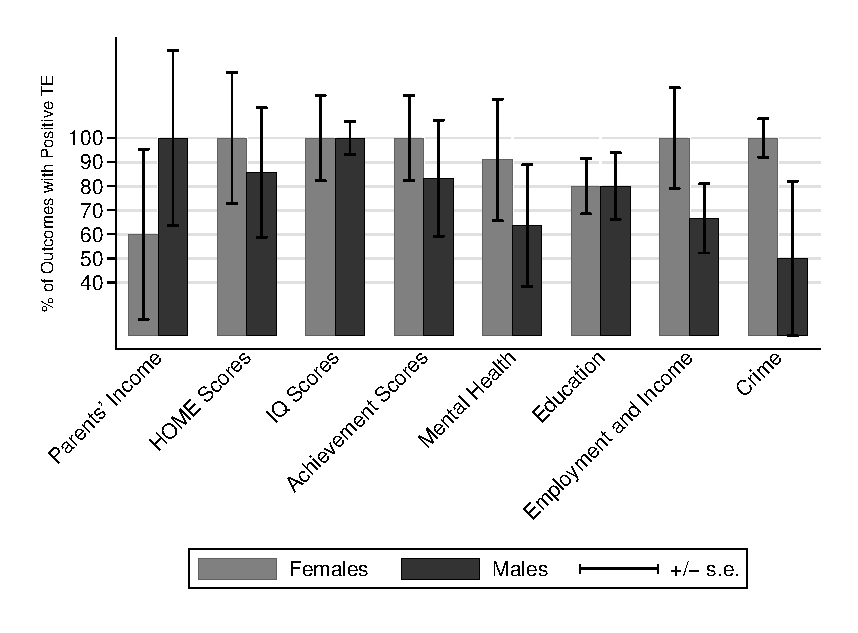
\includegraphics[width=0.8\textwidth]{output/itt_noctrl_cats1}
\end{center}
\end{figure}

\end{frame}

%% ---------------------------------------------------------------------------
\begin{frame}

\begin{figure}[H]
\caption{Percentage of Outcomes with Positive Treatment Effects, Second Set of Categories}
\begin{center}
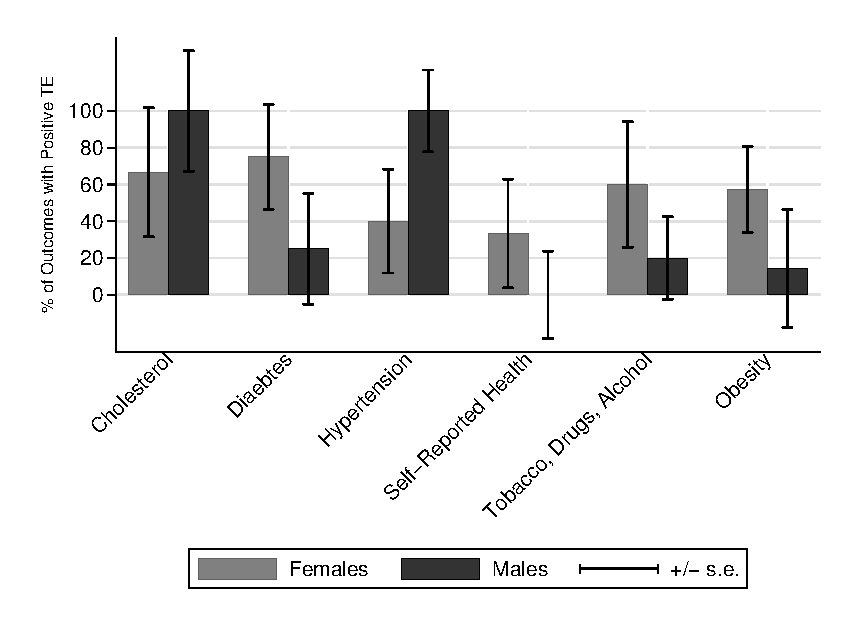
\includegraphics[width=0.8\textwidth]{output/itt_noctrl_cats2}
\end{center}
\end{figure}

\end{frame}

%% ---------------------------------------------------------------------------
\begin{frame}

\begin{figure}[H]
\caption{Percentage of Outcomes with Positive Treatment Effects Fixing Control Group to Stay at Home, First Set of Categories}
\begin{center}
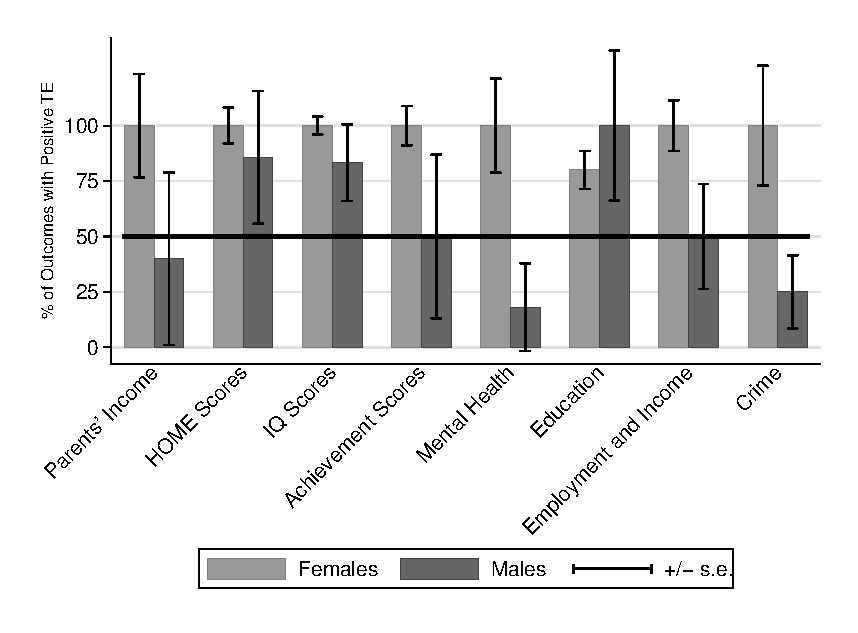
\includegraphics[width=0.8\textwidth]{output/epan_ipw_p0_cats1}
\end{center}
\end{figure}

\end{frame}

%% ---------------------------------------------------------------------------
\begin{frame}

\begin{figure}[H]
\caption{Percentage of Outcomes with Positive Treatment Effects Fixing Control Group to Stay at Home, Second Set of Categories}
\begin{center}
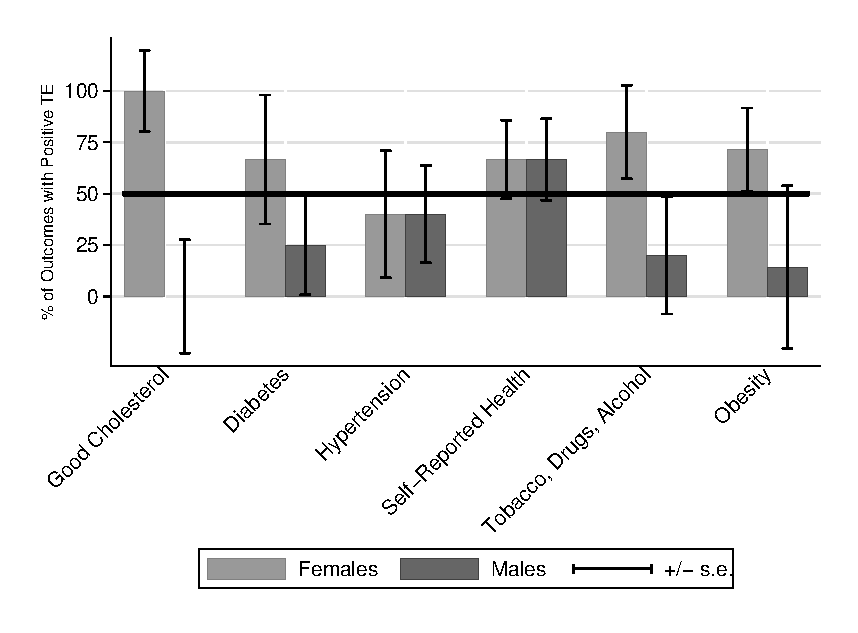
\includegraphics[width=0.8\textwidth]{output/epan_ipw_p0_cats2}
\end{center}
\end{figure}

\end{frame}

%% ---------------------------------------------------------------------------
\begin{frame}

\begin{figure}[H]
\caption{Percentage of Outcomes with Positive Treatment Effects Fixing Control Group to Alternative Preschool, First Set of Categories}
\begin{center}
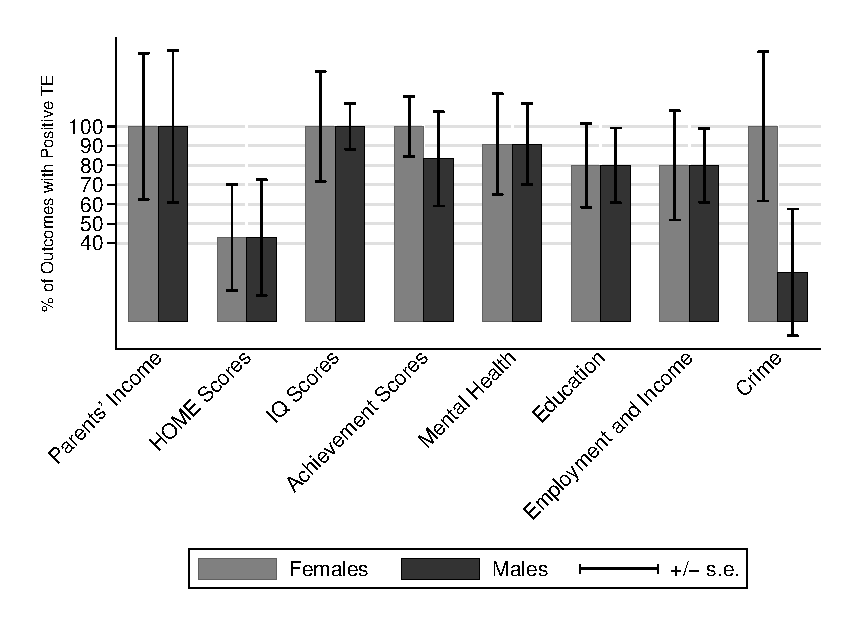
\includegraphics[width=0.8\textwidth]{output/epan_ipw_p1_cats1}
\end{center}
\end{figure}

\end{frame}

%% ---------------------------------------------------------------------------
\begin{frame}

\begin{figure}[H]
\caption{Percentage of Outcomes with Positive Treatment Effects Fixing Control Group to Alternative Preschool, Second Set of Categories}
\begin{center}
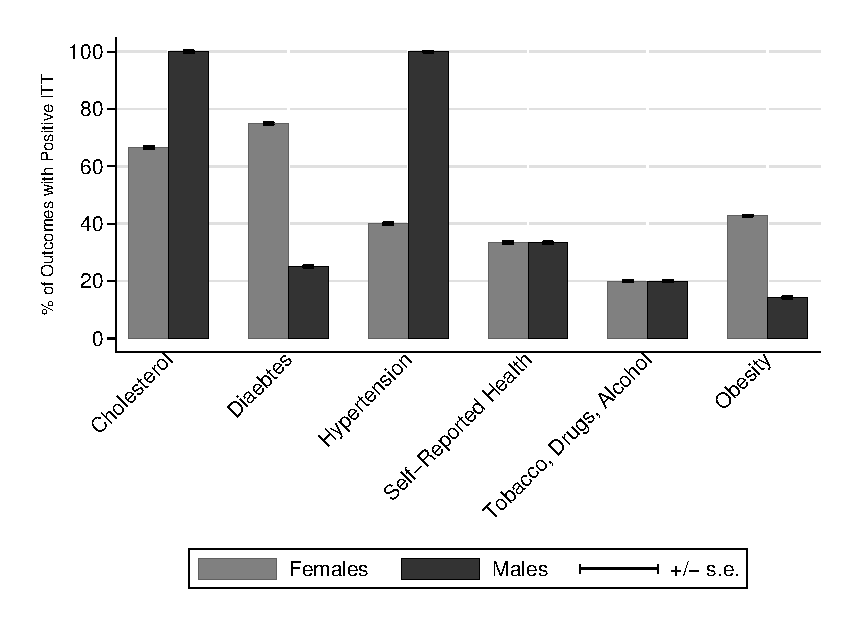
\includegraphics[width=0.8\textwidth]{output/epan_ipw_p1_cats2}
\end{center}
\end{figure}

\end{frame}

\textbf{[JLG: note that there is a figure in which a bar for males doesn't appear. It's not an error. There are no positive effects for that specific counterfactual and for that specific category. It's only one bar. It's males cholesterol when comparing treatment to stay at home.]}

%% ---------------------------------------------------------------------------
\begin{frame}

\begin{center}
\hyperlink{ret:estimated-comb}{\underline{Return to main text}}
\end{center}

\end{frame}

%% ---------------------------------------------------------------------------
{\mode<presentation>{\section[Support]{Common Support between Experimental and Non-Experimental Samples}}}
%-----------------------------------------------------------------------------
\begin{frame}

\hypertarget{doughnut}{}
\begin{center}
\textbf{Common Support between Experimental and Non-Experimental Samples}
\end{center}

\end{frame}

%% ---------------------------------------------------------------------------
\begin{frame}

\begin{itemize}
\item $W$ (pre-program variables) and $X$ (programs possibly affected by treatment).
\item $W =$ {male indicator, black indicator, mother’s education}
\item $X =$ {PIAT scores at ages 5-7, years of education at age 30 income at ages 21 and 30, BMI at age 34}
\item How do we choose the variables in $W,X$?
    \begin{itemize}
    \item Restriction imposed by the availability (overlap) of the the data in the experimental and non-experimental sources
    \item Careful cross-walk to maximize the amount of variables we were able to work with
    \end{itemize}
\end{itemize}

\end{frame}

%% ---------------------------------------------------------------------------

\begin{itemize}
\item The following graphs display the support of ABC, PSID, NLSY79, and CNLSY for variables we use to project future earnings. PIAT math scores are averaged over ages 5--7.
\end{itemize}

%% ---------------------------------------------------------------------------
\begin{frame}

\begin{figure}[H]
\caption{Support of ABC/CARE and Auxiliary Data: Income at Age 21} \label{fig:support}
\begin{center}
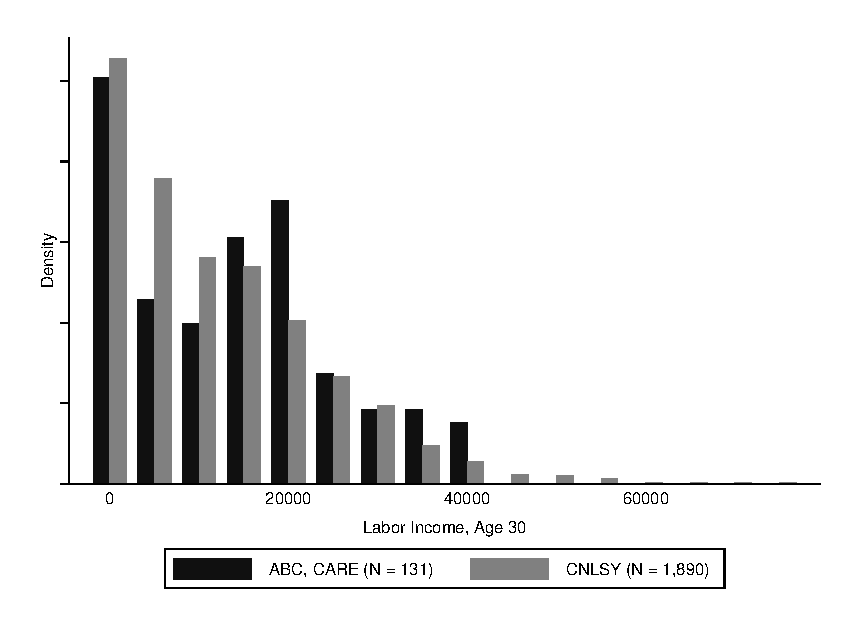
\includegraphics[width=.75\textwidth]{AppOutput/Methodology/support_inc21.eps}
\end{center}
\end{figure}

\end{frame}

%% ---------------------------------------------------------------------------
\begin{frame}

\begin{figure}[H]\addtocounter{figure}{-1}
\caption{Support of ABC/CARE and Auxiliary Data: Income at Age 30} \label{fig:support}
\begin{center}
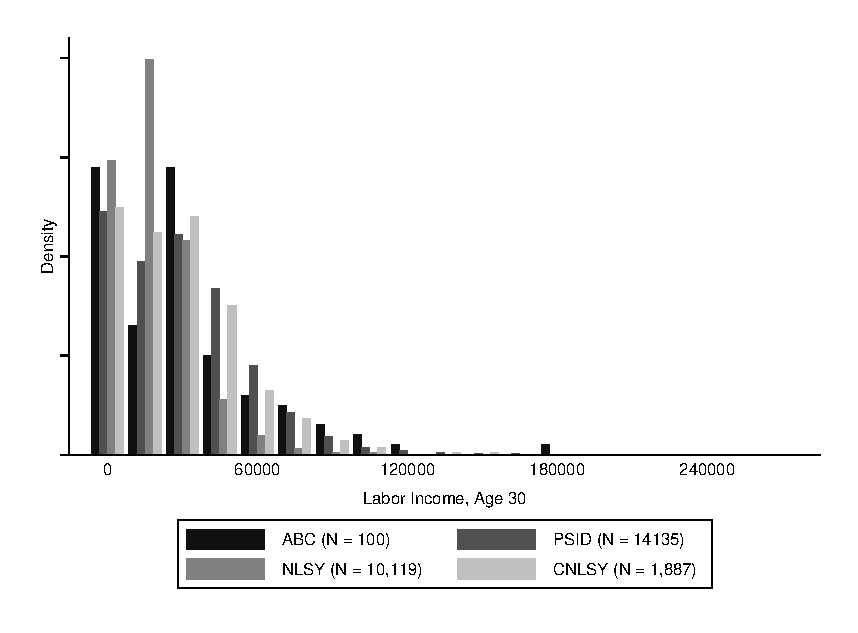
\includegraphics[width=.75\textwidth]{AppOutput/Methodology/support_inc30.eps}
\end{center}
\end{figure}

\end{frame}

%% ---------------------------------------------------------------------------
\begin{frame}

\begin{figure}[H]\addtocounter{figure}{-1}
\caption{Support of ABC/CARE and Auxiliary Data: Subject's Years of Education} \label{fig:support_educ}
\begin{center}
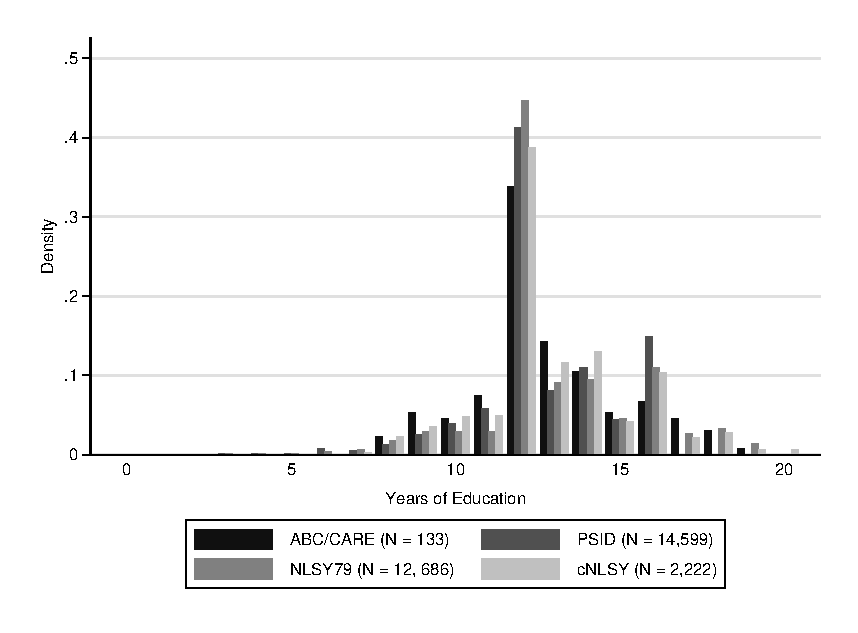
\includegraphics[width=.75\textwidth]{AppOutput/Methodology/support_educ.eps}
\end{center}
\end{figure}

\end{frame}

%% ---------------------------------------------------------------------------
\begin{frame}

\begin{figure}[H]\addtocounter{figure}{-1}
\caption{Support of ABC/CARE and Auxiliary Data: Mother's Years of Education} \label{fig:support_meduc}
\begin{center}
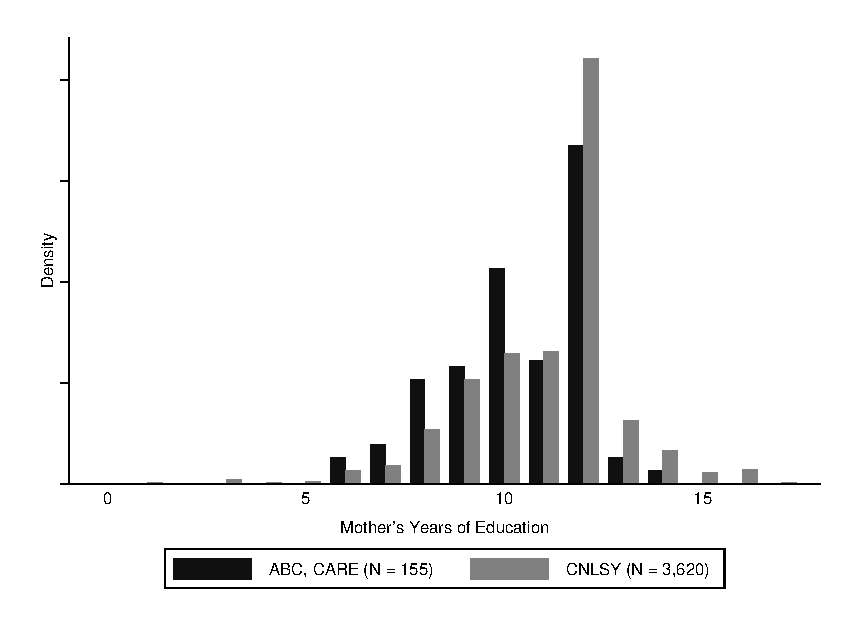
\includegraphics[width=.75\textwidth]{AppOutput/Methodology/support_momed.eps}
\end{center}
\end{figure}

\end{frame}

%% ---------------------------------------------------------------------------
\begin{frame}

\begin{figure}[H]\addtocounter{figure}{-1}
\caption{Support of ABC/CARE and Auxiliary Data: Average PIAT Math Scores, Ages 5--7} \label{fig:support_math}
\begin{center}
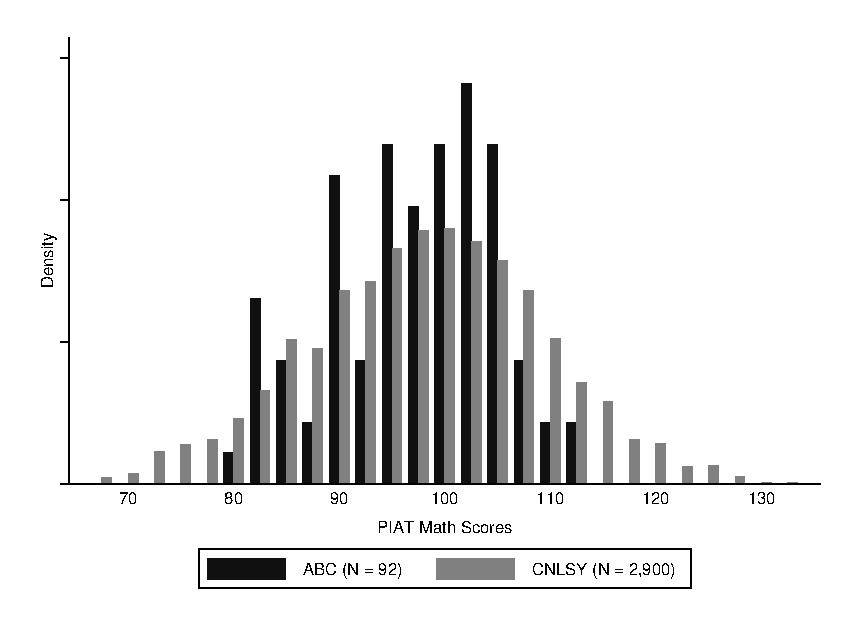
\includegraphics[width=.75\textwidth]{AppOutput/Methodology/support_math.eps}
\end{center}
\end{figure}

\end{frame}

%% ---------------------------------------------------------------------------
\begin{frame}
	
\begin{figure}[H]\addtocounter{figure}{-1}
\caption{Support of ABC/CARE and Auxiliary Data: Body Mass Index, Age 34} \label{fig:support_bmi}
\begin{center}
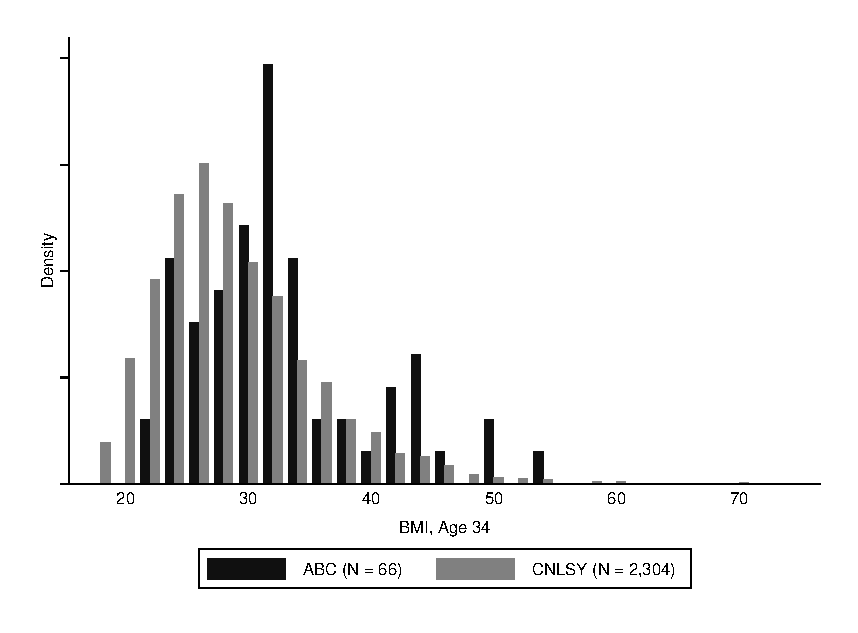
\includegraphics[width=.75\textwidth]{AppOutput/Methodology/support_bmi.eps}
\end{center}
\end{figure}

\end{frame}

%% ---------------------------------------------------------------------------
\begin{frame}

\begin{center}
\hyperlink{ret:doughnut}{\underline{Return to main text}}
\end{center}

\end{frame}

%% ---------------------------------------------------------------------------
{\mode<presentation>{\section[Data]{Full Experimental Data Tables}}}
%-----------------------------------------------------------------------------
\begin{frame}

\hypertarget{potatochips}{}
\begin{center}
\textbf{Full Experimental Data Tables}
\end{center}

\end{frame}

%% ---------------------------------------------------------------------------
\begin{frame}

\begin{table}[H]
\caption{Early Childhood Data (Part I)}\label{tab:ecvars_1}
\begin{center}
\mode<presentation>{\begin{tiny}}
\mode<article>{\begin{scriptsize}}
\begin{tabular}{L{1.4cm} C{2cm} C{1.5cm} C{1.3cm} C{1.3cm}  C{2cm}}
\toprule
\textbf{Category}	&	\textbf{Sub-Category}	&	\textbf{Description}	&	\textbf{ABC Age}  	&  \textbf{CARE Age}  & 	\textbf{Measure}	\\ \midrule
Demographics	&	Gender	&	Gender of subject	&	Birth, 18, 30, 42, 54	&	 Birth, 18, 30, 42, 54	&	Demographic Interview	\\
	&	\\
	&	Race	&	Race/Cultural identity of subject	&	Birth, 18, 30, 42, 54	&	 Birth, 18, 30, 42, 54	&	 Demographic Interview\\
	&	\\
	&	Birth Date	&	Date of birth of subject	&	Birth, 18, 30, 42, 54	& 	Birth, 18, 30, 42, 54	&	 Demographic Interview	\\
\bottomrule
\end{tabular}
\mode<article>{\end{scriptsize}}
\mode<presentation>{\end{tiny}}
\end{center}
\end{table}

\end{frame}

%% ---------------------------------------------------------------------------
\begin{frame}[shrink=5]

\begin{table}[H]
\addtocounter{table}{-1}
\caption{Early Childhood Data (Part I), Cont.}
\begin{center}
\begin{tiny}
\begin{tabular}{L{1.4cm} C{2cm} C{1.5cm} C{1.3cm} C{1.3cm}  C{2cm}}
\toprule
\textbf{Category}	&	\textbf{Sub-Category}	&	\textbf{Description}	&	\textbf{ABC Age}  	&  \textbf{CARE Age}  & 	\textbf{Measure}	\\ \midrule
Cognitive Assessments	&	Language Ability	&	Auditory association, Verbal expression, etc. 	&	36, 42, 48, 54	&	30, 42, 54	&	ITPA$^{ABC}$, GPB$^{ABC}$, PLP$^{ABC}$, MSCD \\
	&	\\
	&	Intelligence Levels	&	SBIS 	&	24, 36, 48, 60	&	24, 36, 48, 60	&	SBIS	\\
	&		&	WPPSI	&	60	&	60	&	WPPSI	\\
	&		&	BSID 	&	3, 6, 9, 12, 18, 24	&	6, 12, 18, 24		&	BSID	\\
	&		&	UOSPD	&	15	&	- 	&	UOSPD$^{ABC}$	\\
	&		&	RPM	&	60	&	-	&	RPM$^{ABC}$	\\
	&	\\
	&	Quantitative	 &	BSID 	&	3, 6, 9, 12, 18, 24	&	6, 12, 18, 24		&	BSID	\\
	&		&	MSCD 	&	30, 42, 54		&	30, 42, 54	&	MSCD	\\
	&	\\
	&	Memory	&	BSID 	&	3, 6, 9, 12, 18, 24	& 	6, 12, 18, 24		&	BSID	\\
	&		&	MSCD 	&	30, 42, 54	&	30, 42, 54	&	MSCD	\\
	&	\\
	&	Motor Development	&	BSID 	&	3, 6, 9, 12, 18, 24	&	6, 12, 18, 24		&	BSID\\
	&		&	MSCD 	&	30, 42, 54	&	30, 42, 54	&	MSCD	\\
	& 	\\
	&	Critical Thinking	&	Curiosity	&	30, 36, 42, 48, 54, 60, 66, 72	& - &	Infant Behavior Inventory$^{ABC}$	\\
\bottomrule
\end{tabular}
\end{tiny}
\end{center}
\end{table}

\end{frame}

%% ---------------------------------------------------------------------------
\begin{frame}

\begin{table}[H]
\addtocounter{table}{-1}
\caption{Early Childhood Data (Part I), Cont.}
\begin{center}
\begin{tiny}
\begin{tabular}{L{1.4cm} C{2cm} C{1.5cm} C{1.3cm} C{1.3cm}  C{2cm}}
\toprule
\textbf{Category}	&	\textbf{Sub-Category}	&	\textbf{Description}	&	\textbf{ABC Age}  	&  \textbf{CARE Age}  & 	\textbf{Measure}	\\ \midrule
Non-Cognitive Assessments	&	Social Skills	&	Positive social response	&	30, 36, 42, 48, 54, 60, 66, 72	&	6, 12, 18, 24		&	Infant Behavior Inventory$^{ABC}$, Bayley Infant Inventory$^{CARE}$	\\
	&		&	Creativity	&	30, 36, 42, 48, 54, 60, 66, 72	&	- 	&	Infant Behavior Inventory$^{ABC}$	\\
	&	\\
	&	Self-Control	&	Locus of control	&	3, 18	&	6, 18	& 	RIES	\\
	&		&	Distractibility, Attentiveness	&	30, 36, 42, 48, 54, 60, 66, 72	&	6, 12, 18, 24		&	Infant Behavior Inventory$^{ABC}$, Bayley Infant Inventory$^{CARE}$	\\
	&	\\
	&	Emotional Health	&	KRT	&	24, 36, 48, 60	&	24, 30, 36, 42, 48, 60	&	KRT	\\
	&	\\
	&	Self-Consciousness	&	Self-consciousness	&	30, 36, 42, 48, 54, 60, 66, 72	&	-	&	Infant Behavior Inventory$^{ABC}$	\\
\bottomrule
\end{tabular}
\end{tiny}
\end{center}
\end{table}

\end{frame}

{\flushleft \normalsize Sources: Authors' description. \\	
Note: This table describes the main categories of variables that were measured for ABC and CARE subjects up to age 6. ABC and CARE ages are measured in months. This is not an exhaustive list of variables, nor does it include variables from auxiliary data. Instruments or questionnaires available for only one of the studies are indicated with the superscript $^{ABC}$ or $^{CARE}$.  \textbf{Abbreviations are as follows.} ITPA: Illinois Test of Psycholinguistic Ability. GPB: Gordon Psycholinguistic Battery. PLP: Preschool Language Performance. MSCD: McCarthy Scales of Children's Development. BSID: Bayley Scales of Infant Development and Infant Behavior. UOSPD: Uzgiris-Hunt Ordinal Scales of Psychological Development. RPM: Raven's Progressive Matrices. RIES: Rotter's Internality-Externality Scale. KRT: Kohn and Rosman Test Behavior Inventory.\\}
\clearpage

%% ---------------------------------------------------------------------------
\begin{frame}

\begin{table}[H]
\caption{Early Childhood Data (Part II)}\label{tab:ecvars_2}
\begin{center}
\begin{tiny}
\begin{tabular}{L{1.3cm} C{1.8cm} C{2cm} C{1.3cm} C{1.3cm}  C{2cm}}
\toprule
\textbf{Category}	&	\textbf{Sub-Category}	&	\textbf{Description}	&	\textbf{ABC Age}  	&  \textbf{CARE Age}  & 	\textbf{Measure}	\\ \midrule
Family Environment	&	Family Members	&	Number of primary caretakers	&	Birth, 18, 30, 42, 54	&	18, 30, 42, 54, 60	&	Demographic Interview	\\
	&		&	Relationship with family members, including father, mother, siblings, etc.	&	Birth, 18, 30, 42, 54	&	18, 30, 42, 54, 60	&	Demographic Interview	\\
	&		&	Number of siblings	&	Birth, 18, 30, 42, 54	&	Birth, 18, 30, 42, 54, 60	&	Demographic Interview	\\
	&		&	Marital status of parents	&	Birth, 18, 30, 42, 54	&	Birth, 18, 30, 42, 54, 60	&	Demographic Interview	\\
	&		&	Marital conflicts between parents	&	6, 18	&	Birth, 6, 18, 36	&	Demographic Interview$^{CARE}$, Parental Attitudes Research Inventory	\\
	&		& Father at home & 18, 30, 42, 54  & 18, 30, 42, 54, 60 & Demographic Interview \\
\bottomrule
\end{tabular}
\end{tiny}
\end{center}
\end{table}

\end{frame}

%% ---------------------------------------------------------------------------
\begin{frame}

\begin{table}[H]
\addtocounter{table}{-1}
\caption{Early Childhood Data (Part II), Cont.}
\begin{center}
\begin{tiny}
\begin{tabular}{L{1.3cm} C{1.8cm} C{2cm} C{1.3cm} C{1.3cm}  C{2cm}}
\toprule
\textbf{Category}	&	\textbf{Sub-Category}	&	\textbf{Description}	&	\textbf{ABC Age}  	&  \textbf{CARE Age}  & 	\textbf{Measure}	\\ \midrule
Family Environment	&	Family Economic Environment	&	Parents' occupation	&	Birth, 18, 30, 42, 54	& 	Birth, 18, 30, 42, 54, 60		&	Demographic Interview	\\
	&								& Mother works & 18, 30, 42, 54 & 18, 30, 42, 54, 60 & Demographic Interview \\
    &		&	Source of child support	&	Birth, 18, 30, 42, 54	&	18, 30, 42, 54, 60	&	Demographic Interview	\\
	&		&	Family income	&	Birth, 18, 30, 42, 54	&	Birth, 18, 30, 42, 54, 60	&	Demographic Interview	\\
	&	\\
	&	Parents and Home Environment & Parents' authority, warmth, family conflict, etc. & 6, 18, 30, 42, 54 & 6, 12, 18, 30, 42, 54 & Parent Interview \\
	&	\\
	&	Family Social Status	&	Parents' education background	&	Birth, 18, 30, 42, 54	&	Birth, 18, 30, 42, 54, 60		&	Demographic Interview	\\
	&		&	Risk taking of family members	&	Birth	&	- 	&	Parent Interview$^{ABC}$	\\
	&	\\
	&	Family Members' Physical Health	&	Health issues of parents	&	Birth	&	Birth	&	Parent Interview	\\
	&		&	Pregnancy history	&	Birth	&	Birth	&	Parent Interview	\\
\bottomrule
\end{tabular}
\end{tiny}
\end{center}
\end{table}

\end{frame}

%% ---------------------------------------------------------------------------
\begin{frame}[shrink=5]

\begin{table}[H]
\addtocounter{table}{-1}
\caption{Early Childhood Data (Part II), Cont.}
\begin{center}
\begin{tiny}
\begin{tabular}{L{1.1cm} C{1.8cm} C{2.2cm} C{1.3cm} C{1.3cm}  C{2cm}}
\toprule
\textbf{Category}	&	\textbf{Sub-Category}	&	\textbf{Description}	&	\textbf{ABC Age}  	&  \textbf{CARE Age}  & 	\textbf{Measure}	\\ \midrule
Childcare	&	Day-care Experience	&	Time and location of childcare, Age when begin	&	Birth, 18, 30, 42, 54	&	18, 30, 42, 54	&	Demographic Interview	\\
			&						& 	Home visits &	-	&	6, 18, 30, 42, 54, 60	& Home Visit Data$^{CARE}$ \\
	&	\\
	&	Parental Care	&	Maternal warmth, Maternal involvement with child	&	6, 18, 30, 42, 54	&	6, 12, 18, 30, 42, 54	&	Home Stimulation	\\
	&		&	Provision of appropriate play materials	&	6, 18, 30, 42, 54	&	 6, 12, 18, 30, 42, 54	&	Home Stimulation	\\
	&		&	Avoidance of restriction and punishment	&	6, 18, 30, 42, 54	&	6, 12, 18, 30		&	Home Stimulation	\\
	&		&	Authoritarian control	&	6, 18, 30, 42, 54	&	6, 12, 18, 30, 36, 42, 102		&	Home Stimulation, Parental Attitudes Research Inventory	\\
	&		&	Democratic attitudes	&	6, 18	&	6, 18, 36	&	Parental Attitudes Research Inventory	\\
	&		&	Hostility and rejection	&	6, 18	&	6, 18, 36	&	Parental Attitudes Research Inventory	\\
	&		&	Parents' knowledge of childcare	&	Birth	&	-	&	Parent Interview$^{ABC}$	\\ \midrule
Physical Health	&	Growth Data	&	Height, Weight, Head circumference, etc.	&	3, 6, 9, 12, 18, 24, 36, 48, 60	&	Birth, 6, 12, 18, 24, 36, 48, 60	&	Growth Measures	\\
\bottomrule
\end{tabular}
\end{tiny}
\end{center}
\end{table}

\end{frame}

{\flushleft \normalsize Sources: Authors' description. \\	
Note: This table describes the main categories of variables that were measured for ABC and CARE subjects up to age 6. ABC and CARE ages are measured in months. This is not an exhaustive list of variables, nor does it include variables from auxiliary data.  Instruments or questionnaires available for only one of the studies are indicated with the superscript $^{ABC}$ or $^{CARE}$.\\}
\clearpage

%%% ---------------------------------------------------------------------------
\begin{frame}

\begin{table}[H]
\caption{Childhood and Adolescent Data (Part I)} \label{tab:youthvars_1}
\begin{center}
\begin{tiny}
\begin{tabular}{L{1.2cm} C{1.4cm} C{2.3cm} C{1cm} C{1cm} C{2.7cm}}
\toprule
\textbf{Category}	&	\textbf{Sub-Category}	&	\textbf{Description}	&	\textbf{ABC Age}  	&  \textbf{CARE Age}  & 	\textbf{Measure}	\\ \midrule
Cognitive Assessment	&	Language Ability	&	Adaptive Language Inventory	&	6, 7, 8	&	6, 7, 8	&	Adaptive Language Inventory	\\
	&		&	Language Questionnaire	&	12	&	- 	&	Language Questionnaire$^{ABC}$	\\
	&		&	MSCD 	&	7	&	- 	&	MSCD$^{ABC}$	\\
	&	\\
	&	Intelligence Tests	&	SBIS	 &	6	&	7	&	SBIS	\\
	&		&	 WIS	&	6, 7, 8, 12, 15	&	6, 8	&	WIS	\\
	&		& Kaufman$^{CARE}$ & 	-	& 6 & Kaufman$^{CARE}$ \\
	&	\\
	&	Quantitative Skills	&	MSCD$^{ABC}$ 	&	7	&	-	&	MSCD$^{ABC}$ 	\\
	&	\\
	&	Memory	&	MSCD$^{ABC}$ 	&	7	&	-	&	MSCD$^{ABC}$	\\
	&	\\
	&	Motor Skills	&	MSCD$^{ABC}$ 	&	7	&	-	&	MSCD$^{ABC}$	\\
\bottomrule
\end{tabular}
\end{tiny}
\end{center}
\end{table}

\end{frame}

%%% ---------------------------------------------------------------------------
\begin{frame}

\begin{table}[H]
\addtocounter{table}{-1}
\caption{Childhood and Adolescent Data (Part I), Cont.}
\begin{center}
\begin{tiny}
\begin{tabular}{L{1.2cm} C{1.4cm} C{2.3cm} C{1cm} C{1cm} C{2.7cm}}
\toprule
\textbf{Category}	&	\textbf{Sub-Category}	&	\textbf{Description}	&	\textbf{ABC Age}  	&  \textbf{CARE Age}  & 	\textbf{Measure}	\\ \midrule
Non-Cognitive Assessment	&	Interpersonal Skills	&	Gets along with people	&	6, 8, 12, 15	& 	8, 12	&	PEI, CAS, PMI$^{ABC}$, SAI$^{ABC}$, Subject Interview$^{ABC}$, Quality Rank$^{CARE}$	\\
	&		&	Relationship with the other sex	&	15	&	- 	&	 SAI$^{ABC}$, Subject What I Am Like (Harter)$^{ABC}$	\\
	&	\\
	&	Critical Thinking	&	Thinks for self, questions things	&	6, 8	 &	8, 12	&	PEI, Harter Child$^{CARE}$, CBI	\\
	&		&	Concept Attainment Kit	&	6, 7, 8	&	- 	&	Concept Attainment Kit$^{ABC}$	\\
	&	\\
	&	Self-Control	&	Distracted in class	&	6, 7, 8, 12, 15	&	12	&	SCAN$^{ABC}$, CBI, WPB$^{ABC}$, PMI$^{ABC}$, SAI$^{ABC}$, Self-Evaluation Inventory$^{ABC}$	\\
	&		&	Locus of control	&	15	&	- 	&	Nowicki-Strickland Data, Pearlin Mastery Scale$^{ABC}$	\\
	&	\\
	&	Work Ethic	&	Task Orientation	&	6, 7, 8, 12, 15	&	6, 7, 8, 9, 12 	&	SCAN$^{ABC}$, CBI, PMI$^{ABC}$		\\
\bottomrule
\end{tabular}
\end{tiny}
\end{center}
\end{table}

\end{frame}

%%% ---------------------------------------------------------------------------
\begin{frame}

\begin{table}[H]
\addtocounter{table}{-1}
\caption{Childhood and Adolescent Data (Part I), Cont.}
\begin{center}
\begin{tiny}
\begin{tabular}{L{1.2cm} C{1.4cm} C{2.3cm} C{1cm} C{1cm} C{2.7cm}}
\toprule
\textbf{Category}	&	\textbf{Sub-Category}	&	\textbf{Description}	&	\textbf{ABC Age}  	&  \textbf{CARE Age}  & 	\textbf{Measure}	\\ \midrule
Non-Cognitive Assessment	&	Emotional Health	&	Harms self, suicidal thoughts	&	8, 12, 15	&	8, 12	 	&	Achenbach Parent,  Subject Risk Taking Survey$^{ABC}$		\\
	&		&	Depression, anxiety, fear, etc.	&	6, 7, 8, 12, 15	&	7, 8, 9, 12	&	KRT, CAS, ETS,  Achenbach Parent	\\
	&	\\
	&	Social Activities	&	Athletic activities	&	8, 12, 15	&	8, 12		&	Achenbach Parent, SAI$^{ABC}$, Subject What I Am Like (Harter)$^{ABC}$, PEI$^{CARE}$	\\
	&		&	Participant of organizations, e.g. religions	&	8, 12, 15	&	8, 12	&	Achenbach Parent, SAI$^{ABC}$, Subject Interview$^{ABC}$	\\
	&		&	Reading list	&	12, 15	&	12	&	CAS, SAI$^{ABC}$	 \\
	&		&	TV/music	&	12, 15	&	12	&	CAS, SAI$^{ABC}$	, Television Checklist$^{ABC}$		\\
	&	\\
	&	Self-Consciousness	&	Self-conscious emotions	&	8, 12, 15	&	8, 12	&	Achenbach Parent, Subject What I Am Like (Harter)	\\ \bottomrule
\end{tabular}
\end{tiny}
\end{center}
\end{table}

\end{frame}

{\flushleft \normalsize Sources: Authors' descriptions. \\
Note: This table describes the main categories of variables that were measured for ABC and CARE subjects at ages 6 to 18. ABC and CARE ages are measured in years. This is not an exhaustive list of variables, nor does it include variables from auxiliary data.  Instruments or questionnaires available for only one of the studies are indicated with the superscript $^{ABC}$ or $^{CARE}$. \textbf{Abbreviations are as follows.}  MSCD: McCarthy Scales of Children's Development. SBIS: Stanford-Binet Intelligence Scale. WIS: Wechsler Intelligence Scale for Children. KRT: Kohn and Rosman Test Behavior Inventory. WJCA: Woodcock-Johnson Test of Cognitive Abilities. PEI: Parents as Educator Interview. CAS: Child Assessment Schedule. PMI: Psychosocial Maturity Inventory. SAI: Social Adjustment Inventory for Children and Adolescents. SCAN: Schedule of Classroom Activity Norms. CBI: Classroom Behavior Inventory. WPB: Walker Problem Behavior Checklist. ETS: Emotional/Activity/Sociability/Impulsivity Temperament Survey. FES: Family Environment Scale. PIAT: Peabody Individual Achievement Test. CAT: California Achievement Test. MARS: Mid-Adolescence Rating Scale Data.\\}
\clearpage

%%% ---------------------------------------------------------------------------
\begin{frame}

\begin{table}[H]
\caption{Childhood and Adolescent Data (Part II)} \label{tab:youthvars_2}
\begin{center}
\begin{tiny}
\begin{tabular}{L{1.2cm} C{1.4cm} C{2.5cm} C{.9cm} C{.8cm} C{2.9cm}}
\toprule
\textbf{Category}	&	\textbf{Sub-Category}	&	\textbf{Description}	&	\textbf{ABC Age}  	&  \textbf{CARE Age}  & 	\textbf{Measure}	\\ \midrule
Family Environment	&	Family Members	&	Number of adults in house	&	6, 8, 12, 15	&	8, 12	&	PEI, Parent Interview, Subject Person In Household$^{ABC}$		\\
	&		&	Relationship with family members, including father, mother, siblings, etc.	&	6, 8, 12, 15	&	8, 12	&	PEI, FES, SAI, Subject Interview$^{ABC}$, Adult Self Report$^{ABC}$, Parent Interview, Achenbach Parent	\\
	&		&	Number of siblings	&	6, 8, 12, 15	&	7, 8, 12	&	PEI$^{ABC}$, Parent Interview	\\
	&		&	Marital status of parents	&	6, 8, 12, 15	&	7, 8, 12	&	PEI$^{ABC}$	, Parent Interview	\\
		&		& Father at home & 18, 30, 42, 54  & 18, 30, 42, 54, 60 & Demographic Interview \\
	&	\\
	&	Parents' Education Style	&	Role of parents in education	&	6, 8	&	8, 12	&	PEI, Parent Interveiw$^{CARE}$	\\
	&		&	Parents' education beliefs \& methods&	6, 8	&	8, 12 	&	PEI, Parent Interview$^{CARE}$		\\
	&		&	Parents' aspiration \& attitudes towards child	&	6, 8, 12, 15	&	8, 12	&	PEI, Parent Interview	\\
\bottomrule
\end{tabular}
\end{tiny}
\end{center}
\end{table}

\end{frame}

%%% ---------------------------------------------------------------------------
\begin{frame}

\begin{table}[H]
\addtocounter{table}{-1}
\caption{Childhood and Adolescent Data (Part II), Cont.}
\begin{center}
\begin{tiny}
\begin{tabular}{L{1.2cm} C{1.4cm} C{2.5cm} C{.9cm} C{.8cm} C{2.9cm}}
\toprule
\textbf{Category}	&	\textbf{Sub-Category}	&	\textbf{Description}	&	\textbf{ABC Age}  	&  \textbf{CARE Age}  & 	\textbf{Measure}	\\ \midrule
Family Environment	&	Family Economic Environment	&	Parents' occupation	&	6, 8, 12, 15	&	7, 8, 12	&	PEI$^{ABC}$, Parent Interview	\\
		&							& Mother works & 9 & 5, 7, 8 & Demographic Interview \\
	&		&	Source of child support	&	6, 8, 12, 15	&	7, 8, 12	&	PEI$^{ABC}$, Parent Interview	\\
	&		&	Family income	&	6, 8, 12, 15	&	7, 8, 12	&	PEI$^{ABC}$, Parent Interview	\\
	&	\\
		&	Parents and Home Environment & Parents' authority, warmth, family conflict, etc. & 8 & 8 & Parent Interview \\
	&	\\
	&	Family Social Status	&	Parents' education background	&	6, 8, 12, 15	&	7, 8, 12	&	PEI$^{ABC}$, Parent Interview	\\
	&		&	Criminal history and risk taking of family members	&	8, 12, 15	&	- 	&	Subject Taylor Life Events$^{ABC}$, Parent Interview$^{ABC}$	\\
	&	\\
	&	Family Members' Physical Health	&	Health issues of adults in house	&	8, 12, 15	&	12	&	Parent Interview, Subject Taylor Life Events$^{ABC}$	\\
\bottomrule
\end{tabular}
\end{tiny}
\end{center}
\end{table}

\end{frame}

%%% ---------------------------------------------------------------------------
\begin{frame}

\begin{table}[H]
\addtocounter{table}{-1}
\caption{Childhood and Adolescent Data (Part II), Cont.}
\begin{center}
\begin{tiny}
\begin{tabular}{L{1.2cm} C{1.4cm} C{2.5cm} C{.9cm} C{.8cm} C{2.9cm}}
\toprule
\textbf{Category}	&	\textbf{Sub-Category}	&	\textbf{Description}	&	\textbf{ABC Age}  	&  \textbf{CARE Age}  & 	\textbf{Measure}	\\ \midrule
Academic Achievements	&	Standardized Tests	&	Reading, mathematics, and language abilities	&	6, 7, 8, 12	&	6, 8, 9,12	&	CAT$^{ABC}$, PIAT$^{ABC}$, WJCA	\\
		&	\\
	&	Performance in Schoolwork	&	Drop in grades	&	12, 15		&	12	&	CAS	\\
	&		&	Lack of interest in school	&	12, 15		&	12	&	CAS	\\
	&		&  Total years in special education & 17 & 11 & Retention and Special Services Data \\
	&		&  Total years retained in school & 17 & 11 & Retention and Special Services Data \\  \midrule
Physical Health	&	Health Issues	&	Health issues of subject	&	8, 12, 15	&	8, 12	&	Achenbach Parent, Subject Interview$^{ABC}$, Adult Self Report$^{ABC}$, PEI$^{CARE}$, Parent Interview$^{CARE}$	\\
	&	\\
	&	Growth	&	Vision, weight, height	&	8	&	8	&	Growth Data	\\
	&	\\
	&	Teenage Pregnancy	&	Teenage Pregnancy	&	15	&	- 	& Subject Interview$^{ABC}$		\\ \midrule
Social Conduct	&	Law Breaking	&	Felony, Time spent incarcerated	&	15	&	- 	&	MARS$^{ABC}$, Subject Interview$^{ABC}$	\\ \bottomrule
\end{tabular}
\end{tiny}
\end{center}
\end{table}

\end{frame}

{\flushleft \normalsize Sources: Authors' descriptions. \\
Note: This table describes the major categories of variables that were measured for ABC and CARE subjects at ages 6 to 18. ABC and CARE age are measured in years. This is not an exhaustive list of variables, nor does it include variables from auxiliary data.  Instruments or questionnaires available for only one of the studies are indicated with the superscript $^{ABC}$ or $^{CARE}$. \textbf{Abbreviations are as follows.}  MSCD: McCarthy Scales of Children's Development. SBIS: Stanford-Binet Intelligence Scale. WIS: Wechsler Intelligence Scale for Children. KRT: Kohn and Rosman Test Behavior Inventory. WJCA: Woodcock-Johnson Test of Cognitive Abilities. PEI: Parents as Educator Interview. CAS: Child Assessment Schedule. PMI: Psychosocial Maturity Inventory. SAI: Social Adjustment Inventory for Children and Adolescents. SCAN: Schedule of Classroom Activity Norms. CBI: Classroom Behavior Inventory. WPB: Walker Problem Behavior Checklist. ETS: Emotional/Activity/Sociability/Impulsivity Temperament Survey. FES: Family Environment Scale. PIAT: Peabody Individual Achievement Test. CAT: California Achievement Test. MARS: Mid-Adolescence Rating Scale Data.\\}
\clearpage

%% ---------------------------------------------------------------------------
\begin{frame}

\begin{table}[H]
\caption{Adult Data (Part I)} \label{tab:adultvars_1}							
\begin{center}
\begin{tiny}					
\begin{tabular}{L{1.2cm} C{1.4cm} C{2.5cm} C{.8cm} C{.8cm} C{2.9cm}}										
\toprule
\textbf{Category}	&	\textbf{Sub-Category}	&	\textbf{Description}	&	\textbf{ABC Age}  	&  \textbf{CARE Age}  & 	\textbf{Measure}	\\ \midrule
Cognitive Assessments   	&	       Intelligence Tests      	&	       WIS     	&	21	&	-	&	       WIS     \\
\midrule										
Non-Cognitive Assessment        	&	       Interpersonal Skills    	&	       Gets along with people  	&	       21, 30  	&	-	&	       Subject Interview   \\
\\										
        	&	       Self-Control    	&	       Locus of control        	&	       21, 30  	&	-	&	       Nowicki-Strickland Data$^{ABC}$, Pearlin Mastery Scale$^{ABC}$  \\
        	&	               	&	       Proud of working, interest in working   	&	       21, 30  	&	21, 30	&	       Job Satisfaction Survey$^{ABC}$, Subject Interview       \\
\\										
        	&	       Emotional Health        	&	       Harms self, suicidal thoughts,	&	21	&	21	&	       Achenbach,  Subject Risk Taking Survey   \\
        	&	               	&	       depression, anxiety, fear, etc. 	&	       21, 30  	&	21, 30	&	       KRT, Achenbach Parent,  CAS, Brief Symptom Inventory, ETS\\
\\										
        	&	       Social Activities       	&	       Athletic activities     	&	21	&	-	&	       Achenbach,  \\
        	&	               	&	       Participant of organizations, e.g. religions    	&	       21, 30  	&	21, 30	&	       Achenbach, Subject Interview        \\
\bottomrule							
\end{tabular}										
\end{tiny}
\end{center}							
\end{table}

\end{frame}

%% ---------------------------------------------------------------------------
\begin{frame}

\begin{table}[H]
\addtocounter{table}{-1}
\caption{Adult Data (Part I), Cont.}						
\begin{center}
\begin{tiny}						
\begin{tabular}{L{1.2cm} C{1.4cm} C{2.5cm} C{.8cm} C{.8cm} C{2.9cm}}										
\toprule
\textbf{Category}	&	\textbf{Sub-Category}	&	\textbf{Description}	&	\textbf{ABC Age}  	&  \textbf{CARE Age}  & 	\textbf{Measure}	\\ \midrule																
Family Environment      	&	       Family Members  	&	       Number of adults in house       	&	21	&	-	&	       Parent Interview$^{ABC}$ , Subject Interview    \\
        	&	               	&	       Relationship with family members, including father, mother, siblings, etc.      	&	       21, 30  	&	30	&	      Parent Interview, Achenbach$^{ABC}$, Subject Interview, Adult Self Report \\
        	&	               	&	       Number of siblings      	&	       21, 30  	&	30	&	       Parent Interview$^{ABC}$ , Subject Interview    \\
        	&	               	&	       Marital status of parents       	&	21	&	-	&	       Parent Interview$^{ABC}$ , Subject Interview    \\
        	&	               	&	       Number of children, childcare basics    	&	       21, 30  	&	30	&	       Subject Interview, Childcare Questionnaire      \\
\\										
        	&	       Family Economic Environment     	&	       Parents' occupation     	&	21	&	-	&	       Parent Interview$^{ABC}$ , Subject Interview    \\
        	&	               	&	       Source of child support 	&	21	&	30	&	       Parent Interview$^{ABC}$ , Subject Interview    \\
        	&	               	&	       Family income   	&	21	&	30	&	       Parent Interview$^{ABC}$ , Subject Interview    \\
\\										
        	&	       Family Members and Children	&	Relationship quality, family health issues, attitude toward child learning	&	30	&	30	&	       Parent Interview, Taylor Life Events$^{ABC}$, Child Health Questionnaire, PEI    \\
\bottomrule							
\end{tabular}										
\end{tiny}
\end{center}							
\end{table}

\end{frame}
\clearpage
%% ---------------------------------------------------------------------------
\begin{frame}

\begin{table}[H]
\addtocounter{table}{-1}
\caption{Adult Data (Part I), Cont.}						
\begin{center}
\begin{tiny}							
\begin{tabular}{L{1.2cm} C{1.4cm} C{2.5cm} C{.8cm} C{.8cm} C{2.9cm}}										
\toprule
\textbf{Category}	&	\textbf{Sub-Category}	&	\textbf{Description}	&	\textbf{ABC Age}  	&  \textbf{CARE Age}  & 	\textbf{Measure}	\\ \midrule								
Family Environment      	&	       Marital Status  	&	       Marital status, spouse income       	&	       21, 30  	&	21, 30	&	       Subject Interview       \\
        	&	               	&	       Spouse details, marriage history	&	       21, 30  	&	30	&	       Subject Interview       \\
        	&	               	&	       Relationship with spouse        	&	       21, 30  	&	30	&	       Subject Interview, Adult Self Report    \\
\\										
 Achievement   	&	       Education Level 	&	       Years in school, plans for future education      	&	       21, 30  	&	       21, 30  	&	       Subject Interview, Adult Self Report    \\
        	&	               	&	       College type, certificate earned        	&	       21, 30  	&	       21, 30  	&	       Subject Interview, Adult Self Report    \\
	&	Achievement Test	&	       WJCA    	&	       21, 30  	&	-	&	       WJCA    \\
	&		&							\\
\bottomrule							
\end{tabular}										
\end{tiny}
\end{center}							
\end{table}

\end{frame}

{\flushleft \normalsize Sources: Authors' description. \\				
Note: This table describes the major categories of variables that were measured for ABC and CARE subjects at ages 21 and 30. ABC and CARE age are measured in years. This is not an exhaustive list of variables, nor does it include variables from auxiliary data. Instruments or questionnaires available for only one of the studies are indicated with the superscript $^{ABC}$ or $^{CARE}$. \textbf{Abbreviations are as follows.} KRT: Kohn and Rosman Test Behavior Inventory. CAS: Child Assessment Schedule. ETS: Emotional/Activity/Sociability/Impulsivity Temperament Survey. WIS: Wechsler Adult Intelligence Scale. WJCA: Woodcock-Johnson Test of Cognitive Abilities. PEI: Parents as Educator Interview.\\}

%% ---------------------------------------------------------------------------
\begin{frame}

\begin{table}[H]
\caption{Adult Data (Part II)} \label{tab:adultvars_2}
\begin{center}
\begin{tiny}
\begin{tabular}{L{1.1cm} C{1.4cm} C{2.5cm} C{.8cm} C{.8cm} C{3cm}}
\toprule
\textbf{Category}	&	\textbf{Sub-Category}	&	\textbf{Description}	&	\textbf{ABC Age}  	&  \textbf{CARE Age}  & 	\textbf{Measure}	\\ \midrule
Physical Health	&	Health Insurance	&	Covered by health insurance	&	21, 30	&	21, 30	&	Subject Interview	\\
\\											
	&	Health Issues	&	Health conditions, diseases, regular checkups and tests, mental health	&	21, 30	&	21	&	Brief Symptom Inventory, Subject Interview, Adult Self Report	\\
\midrule											
Social Conduct	&	Risk Taking	&	Smoking, drinking, carry gun, fight, drug use	&	21, 30	&	21, 30	&	Subject Risk Taking Survey, Adult Self Report	\\
\\											
	&	Law Breaking	&	Felony, Time spent incarcerated	&	21	&	21, 30	& Subject Interview	\\
 \bottomrule
\end{tabular}										
\end{tiny}
\end{center}															
\end{table}

\end{frame}

%% ---------------------------------------------------------------------------
\begin{frame}

\begin{table}[H]
\addtocounter{table}{-1}
\caption{Adult Data (Part II), Cont.}
\begin{center}
\begin{tiny}
\begin{tabular}{L{1.1cm} C{1.4cm} C{2.5cm} C{.8cm} C{.8cm} C{3cm}}
\toprule
\textbf{Category}	&	\textbf{Sub-Category}	&	\textbf{Description}	&	\textbf{ABC Age}  	&  \textbf{CARE Age}  & 	\textbf{Measure}	\\ \midrule										
Economic Status	&	Living Circumstances	&	Number of rooms	&	21, 30	&	21, 30	&	Subject Interview	\\
	&		&	Own or rent apartment	&	21, 30	&	21	&	Subject Interview	\\
	&		&	Number living in same domicile	&	21, 30	&	21	&	Subject Interview	\\
\\											
	&	Working Condition	&	Currently employed	&	21, 30	&	21, 30	&	Subject Interview	\\
	&		&	Job title	&	21, 30	&	21, 30	&	Subject Interview, Adult Self Report	\\
	&		&	Job category	&	21, 30	&	21, 30	&	Subject Interview, Adult Self Report	\\
	&		&	Hours	&	21, 30	&	21, 30	&	Subject Interview, Adult Self Report	\\
	&		&	Satisfied with current job	&	21, 30	&	21, 30	&	Subject Interview, Subject What I Am Like (Harter), Adult Self Report	\\
 \bottomrule
\end{tabular}										
\end{tiny}
\end{center}															
\end{table}

\end{frame}

%% ---------------------------------------------------------------------------
\begin{frame}

\begin{table}[H]
\addtocounter{table}{-1}
\caption{Adult Data (Part II), Cont.}
\begin{center}
\begin{tiny}
\begin{tabular}{L{1.1cm} C{1.4cm} C{2.5cm} C{.8cm} C{.8cm} C{3cm}}
\toprule
\textbf{Category}	&	\textbf{Sub-Category}	&	\textbf{Description}	&	\textbf{ABC Age}  	&  \textbf{CARE Age}  & 	\textbf{Measure}	\\ \midrule										
Economic Status	&	Transportation	&	Own reliable transportation	&	21, 30	&	21	&	Subject Interview, Adult Self Report	\\
	&		&	Public transportation	&	21, 30	&	21	&	Subject Interview, Adult Self Report	\\
\\											
	&	Income	&	Income from job	&	21, 30	&	21, 30	&	Subject Interview, Adult Self Report	\\
	&		&	Income from welfare programs	&	21, 30	&	30	&	Subject Interview, Adult Self Report	\\
	&		&	Income from investment	&	21, 30	&	-	&	Subject Interview, Adult Self Report	\\										
 \bottomrule
\end{tabular}					
\end{tiny}
\end{center}												
\end{table}

\end{frame}

{\flushleft \normalsize Sources: Authors' description. \\				
Note: This table describes the major categories of variables that were measured for ABC and CARE subjects at ages 21 and 30. ABC and CARE age are measured in years. This is not an exhaustive list of variables, nor does it include variables from auxiliary data. Instruments or questionnaires available for only one of the studies are indicated with the superscript $^{ABC}$ or $^{CARE}$.\\}	

%% ---------------------------------------------------------------------------
\begin{frame}

\begin{center}
\hyperlink{ret:potatochips}{\underline{Return to main text}}
\end{center}

\end{frame}
%% ---------------------------------------------------------------------------
{\mode<presentation>{\section[ABC/CARE]{ABC/CARE Tables}}}
%-----------------------------------------------------------------------------
\begin{frame}

\hypertarget{pancakeswaffles}{}
\begin{center}
\textbf{ABC/CARE Tables}
\end{center}

\end{frame}

%% ---------------------------------------------------------------------------
\begin{frame}

\begin{table}[H]
\caption{ABC and CARE, Program Comparison} \label{tab:programcomparison}
\begin{center}
\mode<presentation>{\begin{tiny}}
\mode<article>{\begin{normalsize}}
\begin{tabular}{L{4cm} L{2cm} L{2cm} C{1.5cm}} \toprule
& \multicolumn{1}{c}{ABC}& \multicolumn{1}{c}{CARE} & \multicolumn{1}{c}{ABC = CARE ?} \\ \midrule
\textbf{Program Overview} &&\\
\hspace{.2cm} Years Implemented &1972--1982&1978--1985\\
\hspace{.2cm} First-phase & Birth to 5 years old & Birth to 5 years old &\checkmark \\
\hspace{.2cm} Treatment & & & \\
\hspace{.2cm} Second-phase & 5 to 8 years old & 5 to 8 years old &\checkmark \\
\hspace{.2cm} Treatment & & & \\
\hspace{.2cm} Initially Recruited Sample &121&67\\
\hspace{.2cm} \# of Cohorts &4&2\\
\midrule
\textbf{Eligibility} & Socio-economic disadvantage according to a multi-factor index & Socio-economic disadvantage according to a multi-factor index & \checkmark\\
 \midrule
\textbf{Control} &&\\
\hspace{.2cm} N & 56 & 23\\
\hspace{.2cm} Compensation & Diapers from birth to age 3, unlimited formula from birth to 15 months & Diapers from birth to age 3, unlimited formula from birth to 15 months & \checkmark \\
\hspace{.2cm} Control   & \treatsubsabc & \treatsubscarec \\
\hspace{.2cm} Substitution & & \\
\bottomrule
\end{tabular}
\mode<article>{\end{normalsize}}
\mode<presentation>{\end{tiny}}
\end{center}
{\tiny \flushleft Note: This table compares the main elements of ABC and CARE, summarized in this section. A \checkmark indicates that ABC and CARE had the same feature. A blank space indicates that the indicated component was not part of the program.\\}
\end{table}

\end{frame}

%% ---------------------------------------------------------------------------
\begin{frame}

\begin{table}[H]\addtocounter{table}{-1}
\caption{ABC and CARE, Program Comparison} \label{tab:programcomparison}
\begin{center}
\mode<presentation>{\begin{tiny}}
\mode<article>{\begin{normalsize}}
\begin{tabular}{L{3cm} L{2.5cm} L{3cm} C{1cm}} \toprule
& \multicolumn{1}{c}{ABC}& \multicolumn{1}{c}{CARE} & \multicolumn{1}{c}{ABC = CARE ?} \\ \midrule
\textbf{Treatment} & Center-based childcare & Center-based childcare and family education\\
\hspace{.2cm} \textbf{Center-based} \\
\hspace{.2cm} \textbf{Childcare} \\
\hspace{.2cm} N & 58  & 17 \\
\hspace{.2cm} Intensity &6.5--9.75 hours a day for 50 weeks per year& 6.5--9.75 hours a day for 50 weeks per year & \checkmark\\
\hspace{.2cm} Components & Stimulation, medical care, nutrition, social services & Stimulation, medical care, nutrition, social services & \checkmark\\
\hspace{.2cm} Staff-to-child Ratio &1:3 during ages 0--1 &1:3 during ages 0--1 & \checkmark\\
&1:4--5 during age 1--4 &1:4--5 during age 1--4 & \checkmark\\
&1:5--6 during ages 4--5 & 1:5--6 during ages 4--5 & \checkmark\\
\hspace{.2cm} Staff Qualifications & Range of degrees beyond high school; experience in early childcare & Range of degrees beyond high school; experience in early childcare & \checkmark\\ \\
\bottomrule
\end{tabular}
\mode<article>{\end{normalsize}}
\mode<presentation>{\end{tiny}}
\end{center}
{\tiny \flushleft Note: This table compares the main elements of ABC and CARE, summarized in this section. A \checkmark indicates that ABC and CARE had the same feature. A blank space indicates that the indicated component was not part of the program.\\}
\end{table}

\end{frame}

%% ---------------------------------------------------------------------------
\begin{frame}

\begin{table}[H]\addtocounter{table}{-1}
\caption{ABC and CARE, Program Comparison} \label{tab:programcomparison}
\begin{center}
\mode<presentation>{\begin{tiny}}
\mode<article>{\begin{normalsize}}
\begin{tabular}{L{3cm} L{2.5cm} L{3cm} C{1cm}} \toprule
& \multicolumn{1}{c}{ABC}& \multicolumn{1}{c}{CARE} & \multicolumn{1}{c}{ABC = CARE ?} \\ \midrule
\textbf{Treatment} & Center-based childcare & Center-based childcare and family education\\
\hspace{.2cm} \textbf{Home Visitation}  & & \\
\hspace{.2cm} N & (not part of the program) &27\\
\hspace{.2cm} Intensity && Home visits lasting 1 hour. 2--3 times per month during ages 0--3. 1--2 times per month during ages 4--5\\
\hspace{.2cm} Curriculum & & Social and mental stimulation; parent-child interaction\\
\hspace{.2cm} Staff-to-child Ratio &&1:1\\
\hspace{.2cm} Staff Qualifications &&Home visitor training\\
\bottomrule
\end{tabular}
\mode<article>{\end{normalsize}}
\mode<presentation>{\end{tiny}}
\end{center}
{\tiny \flushleft Note: This table compares the main elements of ABC and CARE, summarized in this section. A \checkmark indicates that ABC and CARE had the same feature. A blank space indicates that the indicated component was not part of the program.\\}
\end{table}

\end{frame}

%% ---------------------------------------------------------------------------
\begin{frame}

\begin{table}[H]\addtocounter{table}{-1}
\caption{ABC and CARE, Program Comparison} \label{tab:programcomparison}
\begin{center}
\mode<presentation>{\begin{tiny}}
\mode<article>{\begin{normalsize}}
\begin{tabular}{L{4cm} L{2cm} L{2cm} C{1.5cm}} \toprule
& \multicolumn{1}{c}{ABC}& \multicolumn{1}{c}{CARE} & \multicolumn{1}{c}{ABC = CARE ?} \\
\midrule
\textbf{School-age Treatment} \\
\hspace{.2cm} Intensity & Every other week& Every other week & \checkmark\\
\hspace{.2cm} Components & Parent-teacher meetings& Parent-teacher meetings & \checkmark\\
\hspace{.2cm} Curriculum & Reading and math &  Reading and math & \checkmark\\
\hspace{.2cm} Staff Qualifications & Range of degrees beyond high school; experience in early childcare & Range of degrees beyond high school; experience in early childcare & \checkmark\\
\bottomrule
\end{tabular}
\mode<article>{\end{normalsize}}
\mode<presentation>{\end{tiny}}
\end{center}
{\tiny \flushleft Note: This table compares the main elements of ABC and CARE, summarized in this section. A \checkmark indicates that ABC and CARE had the same feature. A blank space indicates that the indicated component was not part of the program.\\}
\end{table}

\end{frame}

%% ---------------------------------------------------------------------------
\begin{frame}

\begin{center}
\hyperlink{ret:pancakeswaffles}{\underline{Return to main text}}
\end{center}

\end{frame}

%% ---------------------------------------------------------------------------

\hypertarget{protein}{}
\begin{table}[H]
\caption{Data Availability for ABC and CARE (Part I)} \label{tab:datasumm_1}
\begin{center}
\mode<presentation>{\begin{tiny}}
\mode<article>{\begin{small}}
\begin{tabular}{l c c c} \toprule
Category & Age 0-5 & Age 5-15 & Adult  \\
\midrule
\textbf{Physical Health} \\
\quad Growth data & \CheckmarkBold & - & - \\
\quad Health issues & - & \CheckmarkBold  & \CheckmarkBold \\
\quad Full medical sweep & - & -  & \CheckmarkBold \\
 \midrule
\textbf{Family Environment} \\
\quad Family Members & \CheckmarkBold & \CheckmarkBold & \CheckmarkBold \\
\quad Economic Environment & \CheckmarkBold & \CheckmarkBold & \CheckmarkBold \\
\quad Family Social Status & \CheckmarkBold & \CheckmarkBold & - \\
\quad Family Physical Health & \CheckmarkBold & \CheckmarkBold & - \\
\quad Marital Status/Number of Children & - & - & \CheckmarkBold \\
 \midrule
\textbf{Childcare} \\
\quad Daycare/Parental Care Info & \CheckmarkBold & - & - \\
 \midrule
\textbf{Cognitive Assessments} \\
\quad Intelligence Levels & \CheckmarkBold & \CheckmarkBold & Only ABC \\
\quad Language Ability & \CheckmarkBold & \CheckmarkBold & - \\
\quad Motor Development & \CheckmarkBold & \CheckmarkBold & - \\
\quad Critical Thinking & Only ABC & \CheckmarkBold & - \\
 \bottomrule
\end{tabular}
\mode<article>{\end{small}}
\mode<presentation>{\end{tiny}}
\end{center}
\end{table}

%% ---------------------------------------------------------------------------

\begin{table}[H]
\caption{Data Availability for ABC and CARE (Part II)} \label{tab:datasumm_2}
\begin{center}
\mode<presentation>{\begin{tiny}}
\mode<article>{\begin{small}}
\begin{tabular}{l c c c}  \toprule
Category & Age 0-5 & Age 5-15  & Adult \\
\midrule
\textbf{Non-Cognitive Assessments} \\
\quad Social Skills & \CheckmarkBold & \CheckmarkBold & \CheckmarkBold \\
\quad Self Control & \CheckmarkBold & \CheckmarkBold & Only ABC \\
\quad Self-Consciousness & Only ABC & \CheckmarkBold & - \\
\quad Work Ethic & - & \CheckmarkBold & - \\
\quad Social Activities & - & \CheckmarkBold & \CheckmarkBold \\
 \midrule
\textbf{Academic Achievements} \\
\quad Standardized Tests & - & \CheckmarkBold & - \\
\quad Performance in School & - & \CheckmarkBold & - \\
\quad Education Level & - & - & \CheckmarkBold \\
 \midrule
\textbf{Economic Status} \\
\quad Living Circumstances & - & - & \CheckmarkBold \\
\quad Income/Working Condition & - & - & \CheckmarkBold \\
 \midrule
\textbf{Social Conduct} \\
\quad Administrative Criminal Records & - & - & \CheckmarkBold \\
\quad Law Breaking & - & \CheckmarkBold & \CheckmarkBold \\
\quad Smoking, Drinking, and Drugs & - & - & \CheckmarkBold \\
\bottomrule
\end{tabular}
\mode<article>{\end{small}}
\mode<presentation>{\end{tiny}}
\end{center}
\end{table}

%% ---------------------------------------------------------------------------
\begin{frame}

\begin{center}
\hyperlink{ret:protein}{\underline{Return to main text}}
\end{center}

\end{frame}

%% ---------------------------------------------------------------------------
{\mode<presentation>{\section[Exog.]{Tests of Exogeneity}}}
%-----------------------------------------------------------------------------
\begin{frame}

\hypertarget{tarttarttart}{}
\begin{center}
\textbf{Tests of Exogeneity}
\end{center}

\end{frame}

% ------------------------------------------------------------------------------------------------
\begin{frame}

\begin{block}{}
\begin{center}
\textbf{Testing Assumption~\ref{ass:exog}: Exogeneity}
\end{center}
\end{block}

\end{frame}

%% ------------------------------------------------------------------------------------------------
\begin{frame}

\begin{itemize}
\item The following framework help us to test both Assumptions~\ref{ass:exog} and \ref{ass:summary}.
\item Define an outcome vector as
    \begin{align}
    \bm{Y}_{k,a} &= \bm{X}^d_{k,a} \bm{\gamma} + \bm{\varepsilon}^d_a  &(a) \nonumber
    \end{align}
\end{itemize}

\end{frame}

%% ------------------------------------------------------------------------------------------------
\begin{frame}

\begin{itemize}
\item With an associated measurement system
    \begin{align}  \label{eq:sa-msystemmain}
    \bm{\varepsilon}_{a}^d &=\bm{\beta}^d \bm{\theta}_{a}^d + \bm{\omega}_{a}^d  &(b) \nonumber \\
    \bm{M}_{a}^d &= \bm{\lambda}^d \bm{\theta}_{a}^d + \bm{\eta}_{a^d},  &(c)
    \end{align}
\item where $\bm{\theta}^d \independent \bm{\eta}_{a}^d, \bm{\omega}_{a}^d$ and $\bm{\eta}_{a}^d \independent \bm{\omega}_{a}^d$ for all $a \in \{0, \ldots, A \}, \; d \in \{0,1\}$.
\item We use predictors in these equations.
\item For sake of simplicity, we omit an explicit representation of them here.
\end{itemize}

\end{frame}

%% ------------------------------------------------------------------------------------------------
\begin{frame}

\begin{itemize}
\item When the auxiliary measurement system $\bm{M}_{a}^d $ consists of at least three measures, we are able to identify the vectors of coefficients characterizing this system, $\bm{\lambda}^d, \bm{\beta}^d$, as well as the respective covariance matrices, $\bm{\Sigma}_{\bm{\theta}_{a}^d}, \bm{\Sigma}_{\bm{\eta}_{a}^d}, \bm{\Sigma}_{\bm{\omega}_{a}^d}$, and use the method of \citet{Bartlett_1938_Nature} to obtain an estimate of $\bm{\theta}_{a}^d$ \citep{Heckman_Pinto_etal_2013_PerryFactor}.
\item Identifying and estimating the elements in System \eqref{eq:sa-msystemmain} helps two purposes: (i) propose a test of Assumption~\ref{ass:exog}; and (ii) use estimates of $\bm{\theta}_{a}^d$ as control functions when testing Assumption~\ref{ass:summary} in the next appendix, i.e. use these estimates to ``control'' for endogeneity.
\end{itemize}

\end{frame}

%% ------------------------------------------------------------------------------------------------
\begin{frame}

\begin{itemize}
\item We start by providing estimates for the elements in System~\eqref{eq:sa-msystemmain} in the experimental sample.
\item We assume dedicated measures for these skills at one time period. Put simply, we have two independent systems, one to measure $\bm{\theta}_{c}^d$ and one to measure $\bm{\theta}_{n}^d$, where $\bm{\theta}_{a}^d: = \left[ \bm{\theta}_{c}^d, \bm{\theta}_{n}^d \right]$.
\item We use a set of IQ measures from ages 2 to 8 to obtain an estimate of $\bm{\theta}_{c}^d$ and a set of measures of somatization, hostility, depression, and mental health all at age 21 to measure to estimate $\bm{\theta}_{n}^d$.
\item Figure~\ref{figure:factorsm} shows our estimates by treatment status.
\end{itemize}

\end{frame}

%% ------------------------------------------------------------------------------------------------
\begin{frame}

\begin{figure}[H]
\caption{Estimates of Cognitive ($\theta_{c}^d$) Skills}\label{figure:factorsm}
\begin{center}
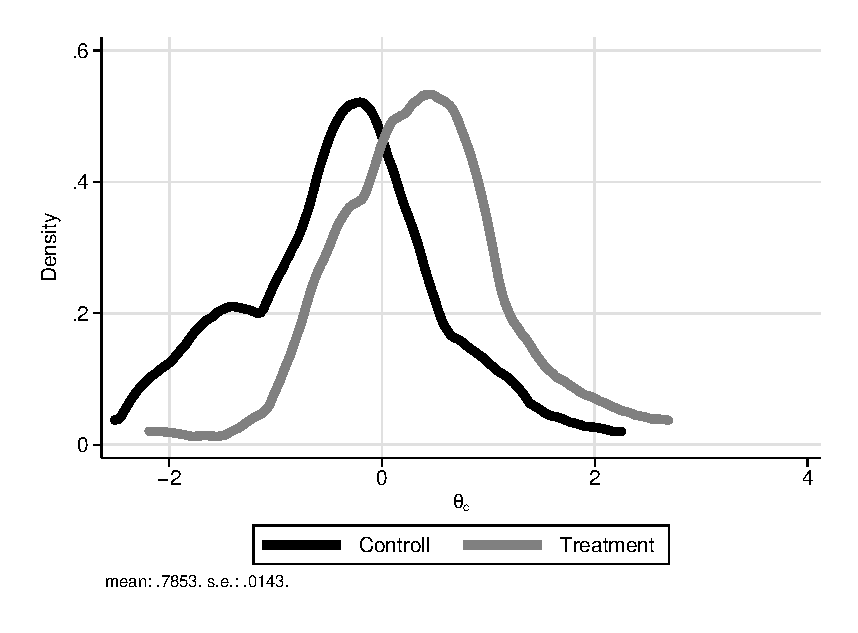
\includegraphics[width=.65\textwidth]{output/abccare_cfactor.eps}
\end{center}
\tiny \flushleft Note: This figure displays a factor score estimated based on the measurement system in \eqref{eq:sa-msystemmain} and measures of IQ at ages 2, 3, 4, 5, 7, and 8 (cognitive skill). Both measures of skills are standardized to a mean of $0$ and a standard deviation of $1$. ``Less'' in the factor measuring non-cognitive skills is ``positive'' given the measures we rely on to construct it. The mean difference between treatment and control is displayed below each panel, with standard error in parentheses. Standard errors are based on the empirical bootstrap distribution.\\
\end{figure}

\end{frame}

%% ------------------------------------------------------------------------------------------------
\begin{frame}

\begin{figure}[H]
\caption{Estimates of Non-cognitive Skills ($\theta_{n}^d$)}\label{fig:c}
\begin{center}
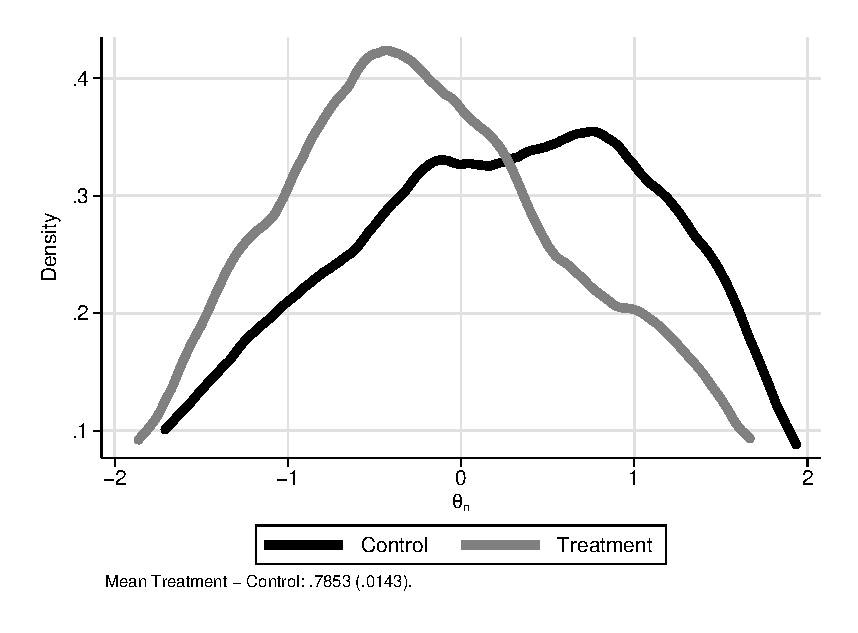
\includegraphics[width=.65\textwidth]{output/abccare_nfactor.eps}
\end{center}
\tiny \flushleft Note: This figure displays an analogous set of graphs for measures of somatization, hostility, depression, and mental health at age 21 (non-cognitive skill). Both measures of skills are standardized to a mean of $0$ and a standard deviation of $1$. ``Less'' in the factor measuring non-cognitive skills is ``positive'' given the measures we rely on to construct it. The mean difference between treatment and control is displayed below each panel, with standard error in parentheses. Standard errors are based on the empirical bootstrap distribution.\\
\end{figure}

\end{frame}

%% ------------------------------------------------------------------------------------------------
\begin{frame}

\begin{itemize}
\item We can also estimate $\bm{\theta}_{a}^d$ in the auxiliary sample.
\item Once these estimates are available, we can test Assumption~\ref{ass:exog} in the experimental and auxiliary samples.
\item The test consists of the following.
\item Let $\bm{\gamma}^E$ be the parameter associated to $\bm{X}^d_{k,a}$ in Equation (a) in System~\eqref{eq:sa-msystemmain} when not accounting for $\bm{\theta}_{a}^d$.
\item Similarly, let $\bm{\gamma}^I$ be the parameter associated with $\bm{X}^d_{k,a}$ in Equation (a) in System~\eqref{eq:sa-msystemmain} when accounting for $\bm{\theta}_{a}^d$.
\item Under the null hypotheses, Assumption~\ref{ass:exog} holds and $\bm{\theta}_{a}^d$ is an irrelevant predictor in Equation (a) in System~\eqref{eq:sa-msystemmain}.
\item This makes the OLS estimate of $\bm{\gamma}^E$ inconsistent.
\end{itemize}

\end{frame}

%% ------------------------------------------------------------------------------------------------
\begin{frame}

\begin{itemize}
\item If the null hypotheses are false, $\bm{X}^d_{k,a}$ and $\varepsilon_{a}^d$ are not independent, $\bm{\gamma}^I$ is consistent and $\bm{\gamma}^E$ is not.
\item We test the null hypothesis by asking if the elements in $\bm{\theta}_{a}^d$ are relevant predictors of a set of outcomes at age 30, so that we can perform the tests both the experimental and the auxiliary samples.
\item We contrast specifications with and without including estimates of $\bm{\theta}_{a}^d$, and report the $F$-statistic corresponding to this comparison.
\item This is a version of a Durbin-Wu-Hausman test \citep[see][]{Durbin_1954_RISI,Wu_1973_Econometrica,Hausman_1978_Econometrica}.
\item Tables~\ref{table:endoginc} to \ref{table:trincome} present the results.
\item In most cases, we are not able to reject the null hypothesis that Assumption~\ref{ass:exog} holds.
\end{itemize}

\end{frame}

%% ------------------------------------------------------------------------------------------------
\begin{frame}

\begin{table}[H]
\caption{Prediction of Labor Income at Age 30 Accounting for $\bm{B}_k$ and $\bm{\theta}, \bm{X}_{k,a}$, ABC/CARE Control Group}\label{table:endoginc}
\begin{center}
\mode<presentation>{\begin{tiny}}
\resizebox{.96\textwidth}{!}{
\begin{tabular}{lcccccccc}
\toprule
 & (1) & (2) & (3) & (4) & (5) & (6) & (7) & (8) \\
 & Estimate & $p$-value & Estimate & $p$-value  & Estimate & $p$-value  & Estimate & $p$-value  \\
 \midrule
Mother's Education &     1,599.57 &         0.17 &       867.41 &         0.34 &      -769.20 &         0.68 &      -580.88 &         0.62 \\
PIAT (5-7) &            . &            . &            . &            . &        45.98 &         0.41 &       423.44 &         0.20 \\
Education (30) &            . &            . &            . &            . &     3,415.53 &         0.03 &     4,505.94 &         0.04 \\
Labor Income (21) &            . &            . &            . &            . &         0.69 &         0.02 &         0.97 &         0.03 \\
Cognitive &            . &            . &       758.28 &         0.43 &            . &            . &    -8,009.28 &         0.93 \\
Non Cognitive &            . &            . &      -342.62 &         0.52 &            . &            . &     7,275.49 &         0.09 \\
Constant &    10,239.82 &         0.28 &    16,530.50 &         0.22 &   -23,140.28 &         0.80 &   -80,679.09 &         0.96 \\  \\
\midrule
$F$-stat &         \multicolumn{2}{c}{2.27} &              \multicolumn{2}{c}{1.80} &             \multicolumn{2}{c}{11.89} &               \multicolumn{2}{c}{7.91}  \\
$p$-value &         \multicolumn{2}{c}{0.42} &              \multicolumn{2}{c}{0.41} &             \multicolumn{2}{c}{0.42} &               \multicolumn{2}{c}{0.01}  \\
$R^2$ &         \multicolumn{2}{c}{0.03} &              \multicolumn{2}{c}{0.07} &             \multicolumn{2}{c}{0.30} &               \multicolumn{2}{c}{0.40}  \\
Observations &         \multicolumn{2}{c}{66} &          \multicolumn{2}{c}{51} &              \multicolumn{2}{c}{65} &             \multicolumn{2}{c}{63}  \\  \\ \midrule
$F$-stat: exclude Cognitive, Non-Cognitive &              \multicolumn{4}{c}{1.70} &               \multicolumn{4}{c}{4.14}  \\
$p$-value  &         \multicolumn{4}{c}{0.45} &                   \multicolumn{4}{c}{0.09} \\
\bottomrule
\end{tabular}
}
\mode<presentation>{\end{tiny}}
\end{center}
\tiny \flushleft
$F$-stat: exclude Cognitive and Non-Cognitive: $F$-statistic contrasting the specifications in columns (1) and (3) and (5) and (7), respectively.\\
Note: Prediction of labor income at age 30 based on the variables listed in the row. Empty cells indicate that the variable was not used in the prediction. For each coefficient we provide point estimate and $p$-value for the treatment and control groups and a test for the treatment-control difference. $\hat{\bm{\theta}}_{c}$: factor score estimated based on the measurement system in \eqref{eq:sa-msystemmain} and measures of IQ at ages 2, 3, 4, 5, 7, and 8 (cognitive skill). $\hat{\bm{\theta}}_{n}$: factor score estimated based on the measurement system in \eqref{eq:sa-msystemmain} and measures of somatization, hostility, depression, and a global mental health index at age 21 (non-cognitive skill). Both measures of skills are standardized to a mean of $0$ and a standard deviation of $1$. Inference is based on the empirical bootstrap distribution. If the estimates for the constant terms are in the ten or hundred thousands, we report a figure that has been rounded to the thousands.\\
\end{table}

\end{frame}

%% ------------------------------------------------------------------------------------------------
\begin{frame}

\begin{table}[H]
\caption{Prediction of Labor Income at Age 30 Accounting for $\bm{B}_k$ and $\bm{\theta}, \bm{X}_{k,a}$, ABC/CARE Treatment Group}
\begin{center}
\mode<presentation>{\begin{tiny}}
\resizebox{.98\textwidth}{!}{
\begin{tabular}{lcccccccc}
\toprule
& (1) & (2) & (3) & (4) & (5) & (6) & (7) & (8) \\
& Estimate & $p$-value & Estimate & $p$-value  & Estimate & $p$-value  & Estimate & $p$-value  \\
\midrule
Mother's Education &     3,134.16 &         0.23 &     2,600.34 &         0.35 &     2,913.44 &         0.28 &     5,835.67 &         0.22 \\
PIAT (5-7) &            . &            . &            . &            . &      -263.29 &         0.66 &      -871.06 &         0.76 \\
Education (30) &            . &            . &            . &            . &    11,600.24 &         0.00 &    13,069.48 &         0.00 \\
Labor Income (21) &            . &            . &            . &            . &        -0.18 &         0.64 &        -0.62 &         0.75 \\
Cognitive &            . &            . &     2,766.35 &         0.40 &            . &            . &     4,828.93 &         0.34 \\
Non Cognitive &            . &            . &     7,600.33 &         0.18 &            . &            . &     6,223.32 &         0.19 \\
Constant &     3,900.73 &         0.47 &    10,553.93 &         0.42 &  -122,709.85 &         0.91 &  -109,410.81 &         0.76 \\  \\
\midrule
$F$-stat &         \multicolumn{2}{c}{1.72} &          \multicolumn{2}{c}{2.45} &          \multicolumn{2}{c}{4.59} &             \multicolumn{2}{c}{4.95} \\
$p$-value &         \multicolumn{2}{c}{0.38} &          \multicolumn{2}{c}{0.21} &          \multicolumn{2}{c}{0.38} &             \multicolumn{2}{c}{0.06} \\
$R^2$ &         \multicolumn{2}{c}{0.02} &          \multicolumn{2}{c}{0.10} &          \multicolumn{2}{c}{0.26} &             \multicolumn{2}{c}{0.33} \\
Observations &         \multicolumn{2}{c}{64} &         \multicolumn{2}{c}{49} &                \multicolumn{2}{c}{65} &       \multicolumn{2}{c}{63}  \\   \\ \midrule
$F$-stat: exclude Cognitive, Non-Cognitive &             \multicolumn{4}{c}{2.49} &              \multicolumn{4}{c}{2.03}  \\
$p$-value &                 \multicolumn{4}{c}{0.21} &                   \multicolumn{4}{c}{0.31}  \\
\bottomrule
\end{tabular}
}
\mode<presentation>{\end{tiny}}
\end{center}
\tiny \flushleft
$F$-stat: exclude Cognitive and Non-Cognitive: $F$-statistic contrasting the specifications in columns (1) and (3) and (5) and (7), respectively.\\
Note: Prediction of labor income at age 30 based on the variables listed in the row. Empty cells indicate that the variable was not used in the prediction. For each coefficient we provide point estimate and $p$-value for the treatment and control groups and a test for the treatment-control difference. $\hat{\bm{\theta}}_{c}$: factor score estimated based on the measurement system in \eqref{eq:sa-msystemmain} and measures of IQ at ages 2, 3, 4, 5, 7, and 8 (cognitive skill). $\hat{\bm{\theta}}_{n}$: factor score estimated based on the measurement system in \eqref{eq:sa-msystemmain} and measures of somatization, hostility, depression, and a global mental health index at age 21 (non-cognitive skill). Both measures of skills are standardized to a mean of $0$ and a standard deviation of $1$. Inference is based on the empirical bootstrap distribution. If the estimates for the constant terms are in the ten or hundred thousands, we report a figure that has been rounded to the thousands.\\
\end{table}

\end{frame}

%% ------------------------------------------------------------------------------------------------
\begin{frame}

\begin{table}[H]
\caption{Prediction of Labor Income at Age 30 Accounting for $\bm{B}_k$ and $\bm{\theta}, \bm{X}_{k,a}$, ABC/CARE Control and Treatment Groups}
\begin{center}
\mode<presentation>{\begin{tiny}}
\resizebox{.95\textwidth}{!}{
\begin{tabular}{lcccccccc}
\toprule
 & (1) & (2) & (3) & (4) & (5) & (6) & (7) & (8) \\
 & Estimate & $p$-value & Estimate & $p$-value  & Estimate & $p$-value  & Estimate & $p$-value  \\
 \midrule
Mother's Education &     2,668.48 &         0.12 &     2,200.35 &         0.25 &       794.11 &         0.36 &     1,724.88 &         0.31 \\
PIAT (5-7) &            . &            . &            . &            . &      -126.19 &         0.67 &      -400.57 &         0.72 \\
Education (30) &            . &            . &            . &            . &     8,601.33 &         0.00 &     9,706.02 &         0.00 \\
Labor Income (21) &            . &            . &            . &            . &         0.14 &         0.37 &         0.21 &         0.37 \\
Cognitive &            . &            . &     4,260.39 &         0.16 &            . &            . &     1,427.18 &         0.44 \\
Non Cognitive &            . &            . &     2,899.66 &         0.25 &            . &            . &     7,557.01 &         0.05 \\
Constant &     4,443.37 &         0.41 &     9,166.30 &         0.38 &   -78,053.28 &         0.95 &   -75,621.84 &         0.87 \\  \\
\midrule
$F$-stat &         \multicolumn{2}{c}{2.50} &          \multicolumn{2}{c}{1.90} &             \multicolumn{2}{c}{5.87} &                 \multicolumn{2}{c}{5.37}  \\
$p$-value &         \multicolumn{2}{c}{0.29} &          \multicolumn{2}{c}{0.31} &             \multicolumn{2}{c}{0.29} &                 \multicolumn{2}{c}{0.01}  \\
$R^2$ &         \multicolumn{2}{c}{0.02} &          \multicolumn{2}{c}{0.04} &             \multicolumn{2}{c}{0.20} &                 \multicolumn{2}{c}{0.25}  \\
Observations &        \multicolumn{2}{c}{132} &        \multicolumn{2}{c}{100} &     \multicolumn{2}{c}{130} &         \multicolumn{2}{c}{133}  \\  \\ \midrule
$F$-stat: exclude Cognitive, Non-Cognitive  &             \multicolumn{4}{c}{2.07} &               \multicolumn{4}{c}{2.92}  \\
$p$-value &                \multicolumn{4}{c}{0.31} &               \multicolumn{4}{c}{0.19}   \\
\bottomrule
\end{tabular}
}
\mode<presentation>{\end{tiny}}
\end{center}
\tiny \flushleft
$F$-stat: exclude Cognitive and Non-Cognitive: $F$-statistic contrasting the specifications in columns (1) and (3) and (5) and (7), respectively.\\
Note: Prediction of labor income at age 30 based on the variables listed in the row. Empty cells indicate that the variable was not used in the prediction. For each coefficient we provide point estimate and $p$-value for the treatment and control groups and a test for the treatment-control difference. $\hat{\bm{\theta}}_{c}$: factor score estimated based on the measurement system in \eqref{eq:sa-msystemmain} and measures of IQ at ages 2, 3, 4, 5, 7, and 8 (cognitive skill). $\hat{\bm{\theta}}_{n}$: factor score estimated based on the measurement system in \eqref{eq:sa-msystemmain} and measures of somatization, hostility, depression, and a global mental health index at age 21 (non-cognitive skill). Both measures of skills are standardized to a mean of $0$ and a standard deviation of $1$. Inference is based on the empirical bootstrap distribution. If the estimates for the constant terms are in the ten or hundred thousands, we report a figure that has been rounded to the thousands.\\
\end{table}

\end{frame}

%% ------------------------------------------------------------------------------------------------
\begin{frame}

\begin{table}[H]
\caption{Prediction of Labor Income at Age 30 Accounting for $\bm{B}_k$ and $\bm{\theta}, \bm{X}_{k,a}$, CNLSY}
\begin{center}
\mode<presentation>{\begin{tiny}}
\resizebox{.95\textwidth}{!}{
\begin{tabular}{lcccccccc}
\toprule
 & (1) & (2) & (3) & (4) & (5) & (6) & (7) & (8) \\
 & Estimate & $p$-value & Estimate & $p$-value  & Estimate & $p$-value  & Estimate & $p$-value  \\
\midrule
Mother's Education &     2,292.54 &         0.00 &     1,528.20 &         0.00 &       117.79 &         0.25 &       -47.06 &         0.50 \\
PIAT (5-7) &            . &            . &            . &            . &       262.38 &         0.00 &       447.61 &         0.00 \\
Education (30) &          . &            . &            . &            . &     3,722.75 &         0.00 &     4,202.69 &         0.00 \\
Labor Income (21) &            . &            . &            . &            . &         0.62 &         0.00 &         0.82 &         0.00 \\
Cognitive &            . &            . &     2,859.63 &         0.00 &            . &            . &    -4,149.19 &         0.88 \\
Non Cognitive &            . &            . &    -2,921.97 &         1.00 &            . &            . &      -590.26 &         0.75 \\
Constant &     2,840.27 &         0.00 &    11,377.06 &         0.00 &   -53,962.05 &         1.00 &   -78,072.63 &         1.00 \\   \\
\midrule
$F$-stat &         \multicolumn{2}{c}{46.92} &              \multicolumn{2}{c}{4.89} &               \multicolumn{2}{c}{83.55} &                \multicolumn{2}{c}{18.31}  \\
$p$-value &         \multicolumn{2}{c}{0.00} &              \multicolumn{2}{c}{0.04} &               \multicolumn{2}{c}{0.00} &                \multicolumn{2}{c}{0.00}  \\
$R^2$ &         \multicolumn{2}{c}{0.03} &              \multicolumn{2}{c}{0.04} &               \multicolumn{2}{c}{0.19} &                \multicolumn{2}{c}{0.33}  \\
Observations &       \multicolumn{2}{c}{1,862} &            \multicolumn{2}{c}{350} &           \multicolumn{2}{c}{1,860} &          \multicolumn{2}{c}{1,862}   \\  \\
\midrule
$F$-stat: exclude Cognitive, Non-Cognitive &                      \multicolumn{4}{c}{4.18} &                      \multicolumn{4}{c}{1.77}   \\
$p$-value &             \multicolumn{4}{c}{0.04} &                  \multicolumn{4}{c}{0.34}  \\
\bottomrule
\end{tabular}
}
\mode<presentation>{\end{tiny}}
\end{center}
\tiny \flushleft
$F$-stat: exclude Cognitive and Non-Cognitive: $F$-statistic contrasting the specifications in columns (1) and (3) and (5) and (7), respectively.\\
Note: Prediction of labor income at age 30 based on the variables listed in the row. Empty cells indicate that the variable was not used in the prediction. For each coefficient we provide point estimate and $p$-value for the treatment and control groups and a test for the treatment-control difference. $\hat{\bm{\theta}}_{c}$: factor score estimated based on the measurement system in \eqref{eq:sa-msystemmain} and measures of reading and comprehension of the PIAT, as weel as the Peabody Picture Vocabulary Test (PPVT) (cognitive skill). $\hat{\bm{\theta}}_{n}$: factor score estimated based on the measurement system in \eqref{eq:sa-msystemmain} and six scales of the Behavior Problems Index (e.g., anxiety, dependency, social behavior) (non-cognitive skill). Both measures of skills are standardized to a mean of $0$ and a standard deviation of $1$. Inference is based on the empirical bootstrap distribution. If the estimates for the constant terms are in the ten or hundred thousands, we report a figure that has been rounded to the thousands.\\
\end{table}

\end{frame}

%% ------------------------------------------------------------------------------------------------
\begin{frame}

\begin{table}[H]
\caption{Prediction of Transfer Income at Age 30 Accounting for $\bm{B}_k$ and $\bm{\theta}, \bm{X}_{k,a}$, ABC/CARE Control Group}\label{table:endoginc}
\begin{center}
\mode<presentation>{\begin{tiny}}
\resizebox{.96\textwidth}{!}{
\begin{tabular}{lcccccccc}
\toprule
 & (1) & (2) & (3) & (4) & (5) & (6) & (7) & (8) \\
 & Estimate & $p$-value & Estimate & $p$-value  & Estimate & $p$-value  & Estimate & $p$-value  \\
 \midrule
Mother's Education &      -413.76 &         0.78 &      -406.14 &         0.69 &        48.75 &         0.49 &        51.97 &         0.47 \\
PIAT (5-7) &            . &            . &            . &            . &        27.10 &         0.29 &      -101.93 &         0.77 \\
Education (30) &            . &            . &            . &            . &      -684.75 &         0.99 &      -693.44 &         0.91 \\
Labor Income (21) &            . &            . &            . &            . &        -0.14 &         0.99 &        -0.15 &         0.93 \\
Cognitive &            . &            . &      -348.53 &         0.69 &            . &            . &     1,696.96 &         0.13 \\
Non Cognitive &            . &            . &     1,622.92 &         0.05 &            . &            . &       887.17 &         0.19 \\
Constant &     6,664.39 &         0.11 &     6,614.39 &         0.18 &     9,942.56 &         0.18 &    22,736.59 &         0.10 \\  \\
\midrule
$F$-stat &          \multicolumn{2}{c}{1.93} &             \multicolumn{2}{c}{2.96} &            \multicolumn{2}{c}{3.53} &              \multicolumn{2}{c}{2.68}   \\
$p$-value &          \multicolumn{2}{c}{0.34} &             \multicolumn{2}{c}{0.15} &            \multicolumn{2}{c}{0.21} &              \multicolumn{2}{c}{0.27}   \\
$R^2$ &          \multicolumn{2}{c}{0.04} &             \multicolumn{2}{c}{0.15} &            \multicolumn{2}{c}{0.21} &              \multicolumn{2}{c}{0.27}   \\
Observations &         \multicolumn{2}{c}{68} &                 \multicolumn{2}{c}{52} &               \multicolumn{2}{c}{70}  &                \multicolumn{2}{c}{70}   \\  \\
\midrule
$F$-stat: exclude Cognitive, Non-Cognitive  &                 \multicolumn{4}{c}{3.38} &              \multicolumn{4}{c}{2.42}  \\
$p$-value &                \multicolumn{4}{c}{0.19} &               \multicolumn{4}{c}{0.27}  \\
\bottomrule
\end{tabular}
}
\mode<presentation>{\end{tiny}}
\end{center}
\tiny \flushleft
$F$-stat: exclude Cognitive and Non-Cognitive: $F$-statistic contrasting the specifications in columns (1) and (3) and (5) and (7), respectively.\\
Note: Prediction of transfer income at age 30 based on the variables listed in the row. Empty cells indicate that the variable was not used in the prediction. For each coefficient we provide point estimate and $p$-value for the treatment and control groups and a test for the treatment-control difference. $\hat{\bm{\theta}}_{c}$: factor score estimated based on the measurement system in \eqref{eq:sa-msystemmain} and measures of IQ at ages 2, 3, 4, 5, 7, and 8 (cognitive skill). $\hat{\bm{\theta}}_{n}$: factor score estimated based on the measurement system in \eqref{eq:sa-msystemmain} and measures of somatization, hostility, depression, and a global mental health index at age 21 (non-cognitive skill). Both measures of skills are standardized to a mean of $0$ and a standard deviation of $1$. Inference is based on the empirical bootstrap distribution. If the estimates for the constant terms are in the ten or hundred thousands, we report a figure that has been rounded to the thousands.\\
\end{table}

\end{frame}

%% ------------------------------------------------------------------------------------------------
\begin{frame}

\begin{table}[H]
\caption{Prediction of Transfer Income at Age 30 Accounting for $\bm{B}_k$ and $\bm{\theta}, \bm{X}_{k,a}$, ABC/CARE Treatment Group}
\begin{center}
\mode<presentation>{\begin{tiny}}
\resizebox{\textwidth}{!}{
\begin{tabular}{lcccccccc}
\toprule
 & (1) & (2) & (3) & (4) & (5) & (6) & (7) & (8) \\
 & Estimate & $p$-value & Estimate & $p$-value  & Estimate & $p$-value  & Estimate & $p$-value  \\
\midrule
Mother'sEducation &      -212.39 &         0.75 &      -336.44 &         0.81 &      -199.39 &         0.74 &      -302.60 &         0.79 \\
PIAT(5-7) &            . &            . &            . &            . &       -46.36 &         0.86 &       -22.41 &         0.65 \\
Education(30) &            . &            . &            . &            . &       -35.62 &         0.56 &       -72.66 &         0.59 \\
LaborIncome(21) &            . &            . &            . &            . &        -0.05 &         0.94 &        -0.05 &         0.90 \\
Cognitive &            . &            . &      -421.59 &         0.75 &            . &            . &      -273.48 &         0.62 \\
Non Cognitive &            . &            . &      -825.26 &         0.95 &            . &            . &      -987.11 &         0.98 \\
Constant &     3,348.22 &         0.16 &     4,937.75 &         0.14 &     9,041.98 &         0.09 &     8,432.47 &         0.18 \\  \\
\midrule
$F$-stat  &          \multicolumn{2}{c}{1.23} &            \multicolumn{2}{c}{2.59} &                  \multicolumn{2}{c}{1.81} &               \multicolumn{2}{c}{2.27}  \\
$p$-value  &          \multicolumn{2}{c}{0.45} &            \multicolumn{2}{c}{0.18} &                  \multicolumn{2}{c}{0.45} &               \multicolumn{2}{c}{0.25}  \\
$R^2$  &          \multicolumn{2}{c}{0.03} &            \multicolumn{2}{c}{0.15} &                  \multicolumn{2}{c}{0.13} &               \multicolumn{2}{c}{0.25}  \\
Observations &        \multicolumn{2}{c}{63} &               \multicolumn{2}{c}{49}  &             \multicolumn{2}{c}{65}  &         \multicolumn{2}{c}{63}  \\   \\
\midrule
$F$-stat: exclude Cognitive, Non-Cognitive &                    \multicolumn{4}{c}{3.08} &                   \multicolumn{4}{c}{2.79}  \\
$p$-value &              \multicolumn{4}{c}{0.20} &                    \multicolumn{4}{c}{0.18}  \\
\bottomrule
\end{tabular}
}
\mode<presentation>{\end{tiny}}
\end{center}
\tiny \flushleft
$F$-stat: exclude Cognitive and Non-Cognitive: $F$-statistic contrasting the specifications in columns (1) and (3) and (5) and (7), respectively.\\
Note: Prediction of transfer income at age 30 based on the variables listed in the row. Empty cells indicate that the variable was not used in the prediction. For each coefficient we provide point estimate and $p$-value for the treatment and control groups and a test for the treatment-control difference. $\hat{\bm{\theta}}_{c}$: factor score estimated based on the measurement system in \eqref{eq:sa-msystemmain} and measures of IQ at ages 2, 3, 4, 5, 7, and 8 (cognitive skill). $\hat{\bm{\theta}}_{n}$: factor score estimated based on the measurement system in \eqref{eq:sa-msystemmain} and measures of somatization, hostility, depression, and a global mental health index at age 21 (non-cognitive skill). Both measures of skills are standardized to a mean of $0$ and a standard deviation of $1$. Inference is based on the empirical bootstrap distribution. If the estimates for the constant terms are in the ten or hundred thousands, we report a figure that has been rounded to the thousands.\\
\end{table}

\end{frame}

%% ------------------------------------------------------------------------------------------------
\begin{frame}

\begin{table}[H]
\caption{Prediction of Transfer Income at Age 30 Accounting for $\bm{B}_k$ and $\bm{\theta}, \bm{X}_{k,a}$, ABC/CARE Control and Treatment Groups}
\begin{center}
\mode<presentation>{\begin{tiny}}
\resizebox{.96\textwidth}{!}{
\begin{tabular}{lcccccccc}
\toprule
 & (1) & (2) & (3) & (4) & (5) & (6) & (7) & (8) \\
 & Estimate & $p$-value & Estimate & $p$-value  & Estimate & $p$-value  & Estimate & $p$-value  \\
 \midrule
Mother's Education &      -299.72 &         0.81 &      -411.12 &         0.85 &      -135.23 &         0.62 &      -211.76 &         0.68 \\
PIAT (5-7) &            . &            . &            . &            . &       -34.90 &         0.81 &       -66.99 &         0.80 \\
Education (30) &            . &            . &            . &            . &      -430.88 &         0.96 &      -453.82 &         0.96 \\
Labor Income (21) &            . &            . &            . &            . &        -0.09 &         1.00 &        -0.08 &         0.96 \\
Cognitive &            . &            . &      -753.98 &         0.93 &            . &            . &       153.54 &         0.42 \\
Non Cognitive &            . &            . &       631.74 &         0.17 &            . &            . &       264.49 &         0.34 \\
Constant &     5,135.83 &         0.06 &     6,460.15 &         0.07 &    13,548.68 &         0.03 &    17,791.02 &         0.05 \\   \\
\midrule
$F$-stat &         \multicolumn{2}{c}{1.78} &         \multicolumn{2}{c}{3.04} &               \multicolumn{2}{c}{3.86} &            \multicolumn{2}{c}{2.75}  \\
$p$-value &         \multicolumn{2}{c}{0.35} &         \multicolumn{2}{c}{0.12} &               \multicolumn{2}{c}{0.35} &            \multicolumn{2}{c}{0.09}  \\
$R^2$ &         \multicolumn{2}{c}{0.02} &         \multicolumn{2}{c}{0.10} &               \multicolumn{2}{c}{0.15} &            \multicolumn{2}{c}{0.18}  \\
Observations &       \multicolumn{2}{c}{133} &           \multicolumn{2}{c}{101} &         \multicolumn{2}{c}{135} &            \multicolumn{2}{c}{133}  \\  \\ \midrule
$F$-stat: exclude Cognitive, Non-Cognitive &              \multicolumn{4}{c}{3.38} &             \multicolumn{4}{c}{1.23}  \\
$p$-value &            \multicolumn{4}{c}{0.17} &               \multicolumn{4}{c}{0.44}  \\
\bottomrule
\end{tabular}
}
\mode<presentation>{\end{tiny}}
\end{center}
\tiny \flushleft
$F$-stat: exclude Cognitive and Non-Cognitive: $F$-statistic contrasting the specifications in columns (1) and (3) and (5) and (7), respectively.\\
Note: Prediction of transfer income at age 30 based on the variables listed in the row. Empty cells indicate that the variable was not used in the prediction. For each coefficient we provide point estimate and $p$-value for the treatment and control groups and a test for the treatment-control difference. $\hat{\bm{\theta}}_{c}$: factor score estimated based on the measurement system in \eqref{eq:sa-msystemmain} and measures of IQ at ages 2, 3, 4, 5, 7, and 8 (cognitive skill). $\hat{\bm{\theta}}_{n}$: factor score estimated based on the measurement system in \eqref{eq:sa-msystemmain} and measures of somatization, hostility, depression, and a global mental health index at age 21 (non-cognitive skill). Both measures of skills are standardized to a mean of $0$ and a standard deviation of $1$. Inference is based on the empirical bootstrap distribution. If the estimates for the constant terms are in the ten or hundred thousands, we report a figure that has been rounded to the thousands.\\
\end{table}

\end{frame}

%% ------------------------------------------------------------------------------------------------
\begin{frame}

\begin{table}[H]
\caption{Prediction of Transfer Income at Age 30 Accounting for $\bm{B}_k$ and $\bm{\theta}, \bm{X}_{k,a}$, CNLSY} \label{table:trincome}
\begin{center}
\mode<presentation>{\begin{tiny}}
\resizebox{.97\textwidth}{!}{
\begin{tabular}{lcccccccc}
\toprule
 & (1) & (2) & (3) & (4) & (5) & (6) & (7) & (8) \\
 & Estimate & $p$-value & Estimate & $p$-value  & Estimate & $p$-value  & Estimate & $p$-value  \\
 \midrule
Mother'sEducation  &       366.18 &         0.38 &    10,450.96 &         0.00 &     2,337.63 &         0.12 &    10,634.87 &         0.00 \\
PIAT(5-7) &            . &            . &            . &            . &      -872.86 &         0.88 &      -364.63 &         0.50 \\
Education(30) &            . &            . &            . &            . &    -8,126.93 &         1.00 &    -6,206.13 &         0.88 \\
LaborIncome(21) &            . &            . &            . &            . &         0.79 &         0.25 &        -0.99 &         1.00 \\
Cognitive&            . &            . &    -9,680.93 &         0.88 &            . &            . &    -5,092.70 &         0.50 \\
NonCognitive &            . &            . &    18,373.65 &         0.03 &            . &            . &     6,585.57 &         0.22 \\
Constant&            . &            . &    20,921.34 &         0.00 &            . &            . &     9,015.29 &         0.12 \\   \\
\midrule
$F$-stat &         \multicolumn{2}{c}{0.14} &               \multicolumn{2}{c}{1.80} &                \multicolumn{2}{c}{1.06} &             \multicolumn{2}{c}{1.17}   \\
$p$-value &         \multicolumn{2}{c}{.75} &               \multicolumn{2}{c}{0.18} &                \multicolumn{2}{c}{0.49} &             \multicolumn{2}{c}{0.37}   \\
$R^2$ &         \multicolumn{2}{c}{0.00} &               \multicolumn{2}{c}{0.02} &                \multicolumn{2}{c}{0.01} &             \multicolumn{2}{c}{0.06}   \\
Observations &       \multicolumn{2}{c}{1,101} &              \multicolumn{2}{c}{239}  &       \multicolumn{2}{c}{1,100} &      \multicolumn{2}{c}{1,099}   \\  \\
\midrule
$F$-stat: exclude Cognitive, Non-Cognitive &                \multicolumn{4}{c}{1.70} &                 \multicolumn{4}{c}{0.71}   \\
$p$-value  &                \multicolumn{4}{c}{0.26} &                \multicolumn{4}{c}{0.52}    \\
\bottomrule
\end{tabular}
}
\mode<presentation>{\end{tiny}}
\end{center}
\tiny \flushleft
$F$-stat: exclude Cognitive and Non-Cognitive: $F$-statistic contrasting the specifications in columns (1) and (3) and (5) and (7), respectively.\\
Note: Prediction of transfer income at age 30 based on the variables listed in the row. Empty cells indicate that the variable was not used in the prediction. For each coefficient we provide point estimate and $p$-value for the treatment and control groups and a test for the treatment-control difference. $\hat{\bm{\theta}}_{c}$: factor score estimated based on the measurement system in \eqref{eq:sa-msystemmain} and measures of IQ at ages 2, 3, 4, 5, 7, and 8 (cognitive skill). $\hat{\bm{\theta}}_{n}$: factor score estimated based on the measurement system in \eqref{eq:sa-msystemmain} and measures of somatization, hostility, depression, and a global mental health index at age 21 (non-cognitive skill). Both measures of skills are standardized to a mean of $0$ and a standard deviation of $1$. Inference is based on the empirical bootstrap distribution. If the estimates for the constant terms are in the ten or hundred thousands, we report a figure that has been rounded to the thousands.\\
\end{table}

\end{frame}

%% ---------------------------------------------------------------------------
\begin{frame}

\begin{center}
\hyperlink{ret:tarttarttart}{\underline{Return to main text}}
\end{center}

\end{frame}

%% ---------------------------------------------------------------------------
{\mode<presentation>{\section[Implications]{Testable Implications}}}
%-----------------------------------------------------------------------------
\begin{frame}

\hypertarget{creamcheese}{}
\begin{center}
\textbf{Testable Implications}
\end{center}

\end{frame}

% ----------------------------------------------------------------------------
\begin{frame}

\begin{block}{}
\begin{center}
\textbf{Testing Assumption~\ref{ass:summary}: Structural Invariance}
\end{center}
\end{block}

\end{frame}

%% ------------------------------------------------------------------------------------------------
\begin{frame}

\mode<article>{\begin{large}}
\begin{itemize}
\item We show that Assumption~\ref{ass:summary}, together with Assumption~\ref{ass:exog}, implies:
    \begin{equation}\label{eq:invariancetestapp}
    \mathbb{E} \left[ Y_{k,j,a}^d | \bm{X}_{k,a}^d  = \bm{x}, \bm{B}_k = \bm{b}, D = d \right] = \mathbb{E} \left[ Y_{k,j,a} | \bm{X}^d_{k,a}  = \bm{x}, \bm{B}_k = \bm{b} \right],
    \end{equation}
    for $a \in \{1,\dots,A\}$, $k \in \{e,n\}$, and $d \in \{0,1\}$.
\end{itemize}
\mode<article>{\end{large}}

\end{frame}

%% ------------------------------------------------------------------------------------------------
\begin{frame}

\begin{itemize}
\item A direct test of this hypothesis is to use the experimental sample and ask if once we account for a set of the variables in $\bm{X}_{k,a}$, $R$ (randomization to treatment assignment in ABC/CARE, which, as discussed in text, is equivalent to $D$) predicts the outcome of interest, conditional on $\bm{B}_k$.
\end{itemize}

\end{frame}

%% ------------------------------------------------------------------------------------------------
\begin{frame}

\begin{table}[H]
\caption{Prediction of High School Graduation at Age 30 Accounting for $R, \bm{B}_k, \bm{\theta},$ and $\bm{X}_{k,a}$ Pooled Sample, ABC/CARE}\label{table:end2}
\begin{center}
\mode<presentation>{\begin{tiny}}
\resizebox{\textwidth}{!}{
\begin{tabular}{lcccccccc}
\toprule
 & (1) & (2) & (3) & (4) & (5) & (6) & (7) & (8) \\
 & Estimate  & $p$-value  & Estimate  & $p$-value  & Estimate  & $p$-value  & Estimate  & $p$-value  \\
 \midrule
$R$ &     0.130 &     0.040 &     0.106 &     0.170 &     0.019 &     0.415 &     0.019 &     0.425 \\
Mother's Education &     0.093 &     0.000 &     0.081 &     0.000 &     0.051 &     0.000 &     0.043 &     0.050 \\
PIAT (5-7) &         . &         . &         . &         . &    -0.005 &     0.910 &    -0.004 &     0.765 \\
Education (30) &         . &         . &         . &         . &     0.119 &     0.000 &     0.124 &     0.000 \\
Labor Income (21) &         . &         . &         . &         . &     0.000 &     0.005 &     0.000 &     0.010 \\
Cognitive &         . &         . &     0.020 &     0.360 &         . &         . &    -0.038 &     0.740 \\
Non Cognitive &         . &         . &    -0.027 &     0.720 &         . &         . &     0.011 &     0.395 \\
Constant &    -0.410 &     0.985 &    -0.283 &     0.865 &    -1.082 &     1.000 &    -1.148 &     0.985 \\  \\
\midrule
$F$-stat &    \multicolumn{2}{c}{14.497} &          \multicolumn{2}{c}{5.819} &         \multicolumn{2}{c}{40.509} &           \multicolumn{2}{c}{25.147} \\
$R^2$ &     \multicolumn{2}{c}{0.151} &          \multicolumn{2}{c}{0.143} &              \multicolumn{2}{c}{0.440} &          \multicolumn{2}{c}{0.434} \\
Observations &   \multicolumn{2}{c}{134} &           \multicolumn{2}{c}{102} &          \multicolumn{2}{c}{135} &         \multicolumn{2}{c}{133} \\  \bottomrule
\end{tabular}
}
\mode<presentation>{\end{tiny}}
\end{center}
\tiny \flushleft
Note: Prediction of high school graduation at age 30 based on the variables listed in the row. Empty cells indicate that the variable was not used in the prediction. For each coefficient we provide point estimate and $p$-value. $\hat{\bm{\theta}}_{c}$: factor score estimated based on the measurement system in \eqref{eq:sa-msystemmain} and PIAT sections that we do not use to predict (reading and comprehension) as well as by the Peabody Picture Vocabulary Test (PPVT) (cognitive skill). $\hat{\bm{\theta}}_{n}$: factor score estimated based on the measurement system in \eqref{eq:sa-msystemmain} and on six scales of the Behavior Problems Index (e.g., anxiety, dependency, social behavior). Inference is based on the empirical bootstrap distribution. If the estimates for the constant terms are in the ten or hundred thousands, we report a figure that has been rounded to the thousands.\\
\end{table}

\end{frame}

%% ------------------------------------------------------------------------------------------------
\begin{frame}

\begin{table}[H]
\caption{Prediction of High School Graduation at Age 30 Accounting for $R, \bm{B}_k, \bm{\theta},$ and $\bm{X}_{k,a}$ Female Sample, ABC/CARE}\label{table:end2}
\begin{center}
\mode<presentation>{\begin{tiny}}
\resizebox{\textwidth}{!}{
\begin{tabular}{lcccccccc}
\toprule
 & (1) & (2) & (3) & (4) & (5) & (6) & (7) & (8) \\
 & Estimate  & $p$-value  & Estimate  & $p$-value  & Estimate  & $p$-value  & Estimate  & $p$-value  \\
 \midrule
$R$ &     0.196 &     0.010 &     0.091 &     0.250 &     0.031 &     0.385 &     0.037 &     0.425 \\
Mother's Education &     0.077 &     0.000 &     0.062 &     0.050 &     0.036 &     0.055 &     0.023 &     0.170 \\
PIAT (5-7) &         . &         . &         . &         . &    -0.008 &     0.860 &    -0.004 &     0.655 \\
Education (30) &         . &         . &         . &         . &     0.093 &     0.000 &     0.102 &     0.005 \\
Labor Income (21) &         . &         . &         . &         . &     0.000 &     0.000 &     0.000 &     0.000 \\
Cognitive &         . &         . &     0.051 &     0.285 &         . &         . &    -0.073 &     0.775 \\
Non Cognitive &         . &         . &    -0.076 &     0.895 &         . &         . &     0.051 &     0.200 \\
Constant &    -0.266 &     0.800 &    -0.065 &     0.540 &    -0.444 &     0.790 &    -0.872 &     0.870 \\  \\
\midrule
$F$-stat &    \multicolumn{2}{c}{10.180} &     \multicolumn{2}{c}{5.545} &          \multicolumn{2}{c}{35.887} &          \multicolumn{2}{c}{31.753} \\
$R^2$ &     \multicolumn{2}{c}{0.172} &         \multicolumn{2}{c}{0.197} &         \multicolumn{2}{c}{0.556} &           \multicolumn{2}{c}{0.612}  \\
Observations &    \multicolumn{2}{c}{68} &         \multicolumn{2}{c}{53} &          \multicolumn{2}{c}{70} &          \multicolumn{2}{c}{70} \\
\bottomrule
\end{tabular}
}
\mode<presentation>{\end{tiny}}
\end{center}
\tiny \flushleft
Note: Prediction of high school graduation at age 30 based on the variables listed in the row. Empty cells indicate that the variable was not used in the prediction. For each coefficient we provide point estimate and $p$-value. $\hat{\bm{\theta}}_{c}$: factor score estimated based on the measurement system in \eqref{eq:sa-msystemmain} and PIAT sections that we do not use to predict (reading and comprehension) as well as by the Peabody Picture Vocabulary Test (PPVT) (cognitive skill). $\hat{\bm{\theta}}_{n}$: factor score estimated based on the measurement system in \eqref{eq:sa-msystemmain} and on six scales of the Behavior Problems Index (e.g., anxiety, dependency, social behavior). Inference is based on the empirical bootstrap distribution. If the estimates for the constant terms are in the ten or hundred thousands, we report a figure that has been rounded to the thousands.\\
\end{table}

\end{frame}

%% ------------------------------------------------------------------------------------------------
\begin{frame}

\begin{table}[H]
\caption{Prediction of High School Graduation at Age 30 Accounting for $R, \bm{B}_k, \bm{\theta},$ and $\bm{X}_{k,a}$ Male Sample, ABC/CARE}\label{table:end2}
\begin{center}
\mode<presentation>{\begin{tiny}}
\resizebox{\textwidth}{!}{
\begin{tabular}{lcccccccc}
\toprule
 & (1) & (2) & (3) & (4) & (5) & (6) & (7) & (8) \\
 & Estimate  & $p$-value  & Estimate  & $p$-value  & Estimate  & $p$-value  & Estimate  & $p$-value  \\
 \midrule
$R$ &     0.084 &     0.220 &     0.146 &     0.140 &     0.088 &     0.190 &     0.067 &     0.305 \\
Mother's Education &     0.116 &     0.000 &     0.131 &     0.000 &     0.057 &     0.045 &     0.072 &     0.095 \\
PIAT (5-7) &         . &         . &         . &         . &     0.000 &     0.470 &    -0.000 &     0.500 \\
Education (30) &         . &         . &         . &         . &     0.152 &     0.000 &     0.156 &     0.000 \\
Labor Income (21) &         . &         . &         . &         . &     0.000 &     0.170 &     0.000 &     0.440 \\
Cognitive &         . &         . &    -0.023 &     0.645 &         . &         . &    -0.009 &     0.525 \\
Non Cognitive &         . &         . &     0.051 &     0.195 &         . &         . &     0.004 &     0.475 \\
Constant &    -0.636 &     0.970 &    -0.824 &     0.950 &    -2.092 &     1.000 &    -2.227 &     0.955 \\  \\ \hline
$F$-stat &    \multicolumn{2}{c}{11.144} &          \multicolumn{2}{c}{6.555} &           \multicolumn{2}{c}{17.009} &    \multicolumn{2}{c}{10.294}  \\
$R^2$ &     \multicolumn{2}{c}{0.190} &            \multicolumn{2}{c}{0.215} &           \multicolumn{2}{c}{0.467} &     \multicolumn{2}{c}{0.460}  \\
Observations &    \multicolumn{2}{c}{67} &           \multicolumn{2}{c}{49} &           \multicolumn{2}{c}{65} &   \multicolumn{2}{c}{70} \\
\bottomrule
\end{tabular}
}
\mode<presentation>{\end{tiny}}
\end{center}
\tiny \flushleft
Note: Prediction of high school graduation at age 30 based on the variables listed in the row. Empty cells indicate that the variable was not used in the prediction. For each coefficient we provide point estimate and $p$-value. $\hat{\bm{\theta}}_{c}$: factor score estimated based on the measurement system in \eqref{eq:sa-msystemmain} and PIAT sections that we do not use to predict (reading and comprehension) as well as by the Peabody Picture Vocabulary Test (PPVT) (cognitive skill). $\hat{\bm{\theta}}_{n}$: factor score estimated based on the measurement system in \eqref{eq:sa-msystemmain} and on six scales of the Behavior Problems Index (e.g., anxiety, dependency, social behavior). Inference is based on the empirical bootstrap distribution. If the estimates for the constant terms are in the ten or hundred thousands, we report a figure that has been rounded to the thousands.\\
\end{table}

\end{frame}

%% ------------------------------------------------------------------------------------------------
\begin{frame}

\begin{table}[H]
\caption{Prediction of Employment at Age 30 Accounting for $R, \bm{B}_k, \bm{\theta},$ and $\bm{X}_{k,a}$ Pooled Sample, ABC/CARE}\label{table:end2}
\begin{center}
\mode<presentation>{\begin{tiny}}
\resizebox{\textwidth}{!}{
\begin{tabular}{lcccccccc}
\toprule
 & (1) & (2) & (3) & (4) & (5) & (6) & (7) & (8) \\
 & Estimate  & $p$-value  & Estimate  & $p$-value  & Estimate  & $p$-value  & Estimate  & $p$-value  \\
 \midrule
$R$ &     0.123 &     0.040 &     0.121 &     0.115 &    -0.008 &     0.550 &     0.057 &     0.265 \\
Mother's Education &     0.033 &     0.060 &     0.017 &     0.230 &     0.031 &     0.150 &     0.029 &     0.155 \\
PIAT (5-7) &         . &         . &         . &         . &     0.008 &     0.020 &     0.012 &     0.060 \\
Education (30) &         . &         . &         . &         . &     0.046 &     0.005 &     0.026 &     0.080 \\
Labor Income (21) &         . &         . &         . &         . &    -0.000 &     0.850 &    -0.000 &     0.875 \\
Cognitive &         . &         . &     0.077 &     0.060 &         . &         . &    -0.016 &     0.595 \\
Non Cognitive &         . &         . &     0.034 &     0.285 &         . &         . &     0.060 &     0.170 \\
Constant &     0.361 &     0.075 &     0.530 &     0.020 &    -0.877 &     0.975 &    -0.966 &     0.895 \\  \\
\midrule
$F$-stat &     \multicolumn{2}{c}{3.903} &              \multicolumn{2}{c}{4.073} &              \multicolumn{2}{c}{5.239} &              \multicolumn{2}{c}{3.979}           \\
$R^2$ &     \multicolumn{2}{c}{0.057} &              \multicolumn{2}{c}{0.124} &              \multicolumn{2}{c}{0.177} &              \multicolumn{2}{c}{0.229}           \\
Observations &   \multicolumn{2}{c}{133} &            \multicolumn{2}{c}{101} &          \multicolumn{2}{c}{135} &            \multicolumn{2}{c}{133}           \\
\bottomrule
\end{tabular}
}
\mode<presentation>{\end{tiny}}
\end{center}
\tiny \flushleft
Note: Prediction of employment at age 30 based on the variables listed in the row. Empty cells indicate that the variable was not used in the prediction. For each coefficient we provide point estimate and $p$-value. $\hat{\bm{\theta}}_{c}$: factor score estimated based on the measurement system in \eqref{eq:sa-msystemmain} and PIAT sections that we do not use to predict (reading and comprehension) as well as by the Peabody Picture Vocabulary Test (PPVT) (cognitive skill). $\hat{\bm{\theta}}_{n}$: factor score estimated based on the measurement system in \eqref{eq:sa-msystemmain} and on six scales of the Behavior Problems Index (e.g., anxiety, dependency, social behavior). Inference is based on the empirical bootstrap distribution. If the estimates for the constant terms are in the ten or hundred thousands, we report a figure that has been rounded to the thousands.\\
\end{table}

\end{frame}

%% ------------------------------------------------------------------------------------------------
\begin{frame}

\begin{table}[H]
\caption{Prediction of Employment at Age 30 Accounting for $R, \bm{B}_k, \bm{\theta},$ and $\bm{X}_{k,a}$ Female Sample, ABC/CARE}\label{table:end2}
\begin{center}
\mode<presentation>{\begin{tiny}}
\resizebox{\textwidth}{!}{
\begin{tabular}{lcccccccc}
\toprule
 & (1) & (2) & (3) & (4) & (5) & (6) & (7) & (8) \\
 & Estimate  & $p$-value  & Estimate  & $p$-value  & Estimate  & $p$-value  & Estimate  & $p$-value  \\
\midrule
$R$ &     0.124 &     0.135 &     0.003 &     0.495 &    -0.078 &     0.705 &    -0.092 &     0.745 \\
Mother's Education &    -0.000 &     0.520 &    -0.000 &     0.500 &    -0.012 &     0.670 &    -0.000 &     0.500 \\
PIAT (5-7) &         . &         . &         . &         . &     0.010 &     0.030 &     0.008 &     0.145 \\
Education (30) &         . &         . &         . &         . &     0.040 &     0.035 &     0.030 &     0.085 \\
Labor Income (21) &         . &         . &         . &         . &     0.000 &     0.260 &    -0.000 &     0.520 \\
Cognitive &         . &         . &     0.151 &     0.005 &         . &         . &     0.065 &     0.240 \\
Non Cognitive &         . &         . &    -0.027 &     0.655 &         . &         . &     0.019 &     0.425 \\
Constant &     0.702 &     0.000 &     0.754 &     0.000 &    -0.624 &     0.865 &    -0.359 &     0.655 \\  \\
\midrule
$F$-stat &     \multicolumn{2}{c}{1.873} &              \multicolumn{2}{c}{5.089} &              \multicolumn{2}{c}{3.432} &              \multicolumn{2}{c}{3.918} \\
$R^2$ &     \multicolumn{2}{c}{0.048} &              \multicolumn{2}{c}{0.207} &              \multicolumn{2}{c}{0.229} &              \multicolumn{2}{c}{0.289} \\
Observations &    \multicolumn{2}{c}{67} &             \multicolumn{2}{c}{52} &             \multicolumn{2}{c}{65}  &             \multicolumn{2}{c}{70}   \\
\bottomrule
\end{tabular}
}
\mode<presentation>{\end{tiny}}
\end{center}
\tiny \flushleft
Note: Prediction of employment at age 30 based on the variables listed in the row. Empty cells indicate that the variable was not used in the prediction. For each coefficient we provide point estimate and $p$-value. $\hat{\bm{\theta}}_{c}$: factor score estimated based on the measurement system in \eqref{eq:sa-msystemmain} and PIAT sections that we do not use to predict (reading and comprehension) as well as by the Peabody Picture Vocabulary Test (PPVT) (cognitive skill). $\hat{\bm{\theta}}_{n}$: factor score estimated based on the measurement system in \eqref{eq:sa-msystemmain} and on six scales of the Behavior Problems Index (e.g., anxiety, dependency, social behavior). Inference is based on the empirical bootstrap distribution. If the estimates for the constant terms are in the ten or hundred thousands, we report a figure that has been rounded to the thousands.\\
\end{table}

\end{frame}

%% ------------------------------------------------------------------------------------------------
\begin{frame}

\begin{table}[H]
\caption{Prediction of Employment at Age 30 Accounting for $R, \bm{B}_k, \bm{\theta},$ and $\bm{X}_{k,a}$ Male Sample, ABC/CARE}\label{table:end2}
\begin{center}
\mode<presentation>{\begin{tiny}}
\resizebox{\textwidth}{!}{
\begin{tabular}{lcccccccc}
\toprule
 & (1) & (2) & (3) & (4) & (5) & (6) & (7) & (8) \\
 & Estimate  & $p$-value  & Estimate  & $p$-value  & Estimate  & $p$-value  & Estimate  & $p$-value  \\
 \midrule
$R$ &     0.132 &     0.065 &     0.228 &     0.035 &     0.083 &     0.220 &     0.271 &     0.005 \\
Mother's Education &     0.066 &     0.020 &     0.045 &     0.150 &     0.094 &     0.020 &     0.116 &     0.000 \\
PIAT (5-7) &         . &         . &         . &         . &     0.008 &     0.090 &     0.022 &     0.015 \\
Education (30) &         . &         . &         . &         . &     0.023 &     0.235 &    -0.009 &     0.635 \\
LaborIncome (21) &         . &         . &         . &         . &    -0.000 &     0.990 &    -0.000 &     0.940 \\
Cognitive &         . &         . &    -0.030 &     0.665 &         . &         . &    -0.180 &     0.970 \\
Non Cognitive &         . &         . &     0.110 &     0.020 &         . &         . &     0.138 &     0.030 \\
Constant &    -0.002 &     0.500 &     0.203 &     0.350 &    -1.202 &     0.940 &    -2.416 &     0.975 \\  \\
\midrule
$F$-stat &     \multicolumn{2}{c}{4.050} &             \multicolumn{2}{c}{3.140} &              \multicolumn{2}{c}{3.899} &              \multicolumn{2}{c}{5.322} \\
$R^2$ &     \multicolumn{2}{c}{0.114} &            \multicolumn{2}{c}{0.192} &             \multicolumn{2}{c}{0.240} &              \multicolumn{2}{c}{0.443} \\
Observations &    \multicolumn{2}{c}{66} &            \multicolumn{2}{c}{49} &             \multicolumn{2}{c}{65} &             \multicolumn{2}{c}{63} \\
\bottomrule
\end{tabular}
}
\mode<presentation>{\end{tiny}}
\end{center}
\tiny \flushleft
Note: Prediction of employment at age 30 based on the variables listed in the row. Empty cells indicate that the variable was not used in the prediction. For each coefficient we provide point estimate and $p$-value. $\hat{\bm{\theta}}_{c}$: factor score estimated based on the measurement system in \eqref{eq:sa-msystemmain} and PIAT sections that we do not use to predict (reading and comprehension) as well as by the Peabody Picture Vocabulary Test (PPVT) (cognitive skill). $\hat{\bm{\theta}}_{n}$: factor score estimated based on the measurement system in \eqref{eq:sa-msystemmain} and on six scales of the Behavior Problems Index (e.g., anxiety, dependency, social behavior). Inference is based on the empirical bootstrap distribution. If the estimates for the constant terms are in the ten or hundred thousands, we report a figure that has been rounded to the thousands.\\
\end{table}

\end{frame}

%% ------------------------------------------------------------------------------------------------
\begin{frame}

\begin{table}[H]
\caption{Prediction of Labor Income at Age 30 Accounting for $R, \bm{B}_k, \bm{\theta},$ and $\bm{X}_{k,a}$ Pooled Sample, ABC/CARE}\label{table:end2}
\begin{center}
\mode<presentation>{\begin{tiny}}
\resizebox{\textwidth}{!}{
\begin{tabular}{lcccccccc}
\toprule
 & (1) & (2) & (3) & (4) & (5) & (6) & (7) & (8) \\
 & Estimate  & $p$-value  & Estimate  & $p$-value  & Estimate  & $p$-value  & Estimate  & $p$-value  \\
 \midrule
$R$ & 10576.303 &     0.065 & 11,165.829 &     0.125 &   283.356 &     0.490 &  1,836.270 &     0.410 \\
Mother's Education &  1,851.130 &     0.205 &  1,131.843 &     0.375 &   496.581 &     0.430 &  1,052.668 &     0.365 \\
PIAT (5-7) &         &         &         &         &   -81.009 &     0.595 &  -320.784 &     0.705 \\
Education (30) &         &         &         &         &  8,097.138 &     0.000 &  9,141.309 &     0.000 \\
Labor Income (21) &         &         &         &         &     0.130 &     0.330 &     0.192 &     0.325 \\
Cognitive &         &         &  2,308.860 &     0.305 &         &         &   785.891 &     0.465 \\
Non Cognitive &         &         &  2,665.092 &     0.190 &         &         &  6,876.181 &     0.065 \\
Constant &  7,067.552 &     0.405 & 14,188.359 &     0.340 & -73,300.00 &     0.965 & -70,500.00 &     0.920 \\ \\
\midrule
$F$-stat &     1.965 &         &     1.522 &         &     5.746 &         &     4.742 &         \\
$R^2$ &     0.031 &         &     0.056 &         &     0.210 &         &     0.251 &         \\
Observations &   132.000 &         &   101.000 &         &   130.000 &         &   133.000 &         \\
\bottomrule
\end{tabular}
}
\mode<presentation>{\end{tiny}}
\end{center}
\tiny \flushleft
Note: Prediction of employment at age 30 based on the variables listed in the row. Empty cells indicate that the variable was not used in the prediction. For each coefficient we provide point estimate and $p$-value. $\hat{\bm{\theta}}_{c}$: factor score estimated based on the measurement system in \eqref{eq:sa-msystemmain} and PIAT sections that we do not use to predict (reading and comprehension) as well as by the Peabody Picture Vocabulary Test (PPVT) (cognitive skill). $\hat{\bm{\theta}}_{n}$: factor score estimated based on the measurement system in \eqref{eq:sa-msystemmain} and on six scales of the Behavior Problems Index (e.g., anxiety, dependency, social behavior). Inference is based on the empirical bootstrap distribution. If the estimates for the constant terms are in the ten or hundred thousands, we report a figure that has been rounded to the thousands.\\
\end{table}

\end{frame}

%% ------------------------------------------------------------------------------------------------
\begin{frame}

\begin{table}[H]
\caption{Prediction of Labor Income at Age 30 Accounting for $R, \bm{B}_k, \bm{\theta},$ and $\bm{X}_{k,a}$ Female Sample, ABC/CARE}\label{table:end2}
\begin{center}
\mode<presentation>{\begin{tiny}}
\resizebox{\textwidth}{!}{
\begin{tabular}{lcccccccc}
\toprule
 & (1) & (2) & (3) & (4) & (5) & (6) & (7) & (8) \\
 & Estimate  & $p$-value  & Estimate  & $p$-value  & Estimate  & $p$-value  & Estimate  & $p$-value  \\
 \midrule
$R$ &  3,401.892 &     0.305 &  1,194.706 &     0.410 & -6,899.006 &     0.915 & -5,862.320 &     0.840 \\
Mother's Education &  -852.061 &     0.675 & -1,688.467 &     0.835 & -2,581.049 &     0.975 & -2,473.902 &     0.965 \\
PIAT (5-7) &         &         &         &         &   260.764 &     0.165 &   347.907 &     0.170 \\
Education (30) &         &         &         &         &  3,580.642 &     0.000 &  3,916.084 &     0.005 \\
LaborIncome (21) &         &         &         &         &     0.329 &     0.175 &     0.392 &     0.160 \\
Cognitive &         &         &  3,828.286 &     0.130 &         &         & -2,905.637 &     0.785 \\
Non Cognitive &         &         & -1,663.392 &     0.655 &         &         &  2,051.882 &     0.300 \\
Constant & 32,117.510 &     0.055 & 39,943.031 &     0.025 & -21,500.00 &     0.800 & -36,600.00 &     0.840 \\  \\
\midrule
$F$-stat &     1.234 &         &     2.812 &         &     9.052 &         &     8.916 &         \\
$R^2$ &     0.039 &         &     0.143 &         &     0.354 &         &     0.393 &         \\
Observations &    67 &         &    52 &         &    65 &         &    70 &         \\
\bottomrule
\end{tabular}
}
\mode<presentation>{\end{tiny}}
\end{center}
\tiny \flushleft
Note: Prediction of labor income at age 30 based on the variables listed in the row. Empty cells indicate that the variable was not used in the prediction. For each coefficient we provide point estimate and $p$-value. $\hat{\bm{\theta}}_{c}$: factor score estimated based on the measurement system in \eqref{eq:sa-msystemmain} and PIAT sections that we do not use to predict (reading and comprehension) as well as by the Peabody Picture Vocabulary Test (PPVT) (cognitive skill). $\hat{\bm{\theta}}_{n}$: factor score estimated based on the measurement system in \eqref{eq:sa-msystemmain} and on six scales of the Behavior Problems Index (e.g., anxiety, dependency, social behavior). Inference is based on the empirical bootstrap distribution. If the estimates for the constant terms are in the ten or hundred thousands, we report a figure that has been rounded to the thousands.\\
\end{table}

\end{frame}

%% ------------------------------------------------------------------------------------------------
\begin{frame}

\begin{table}[H]
\caption{Prediction of Labor Income at Age 30 Accounting for $R, \bm{B}_k, \bm{\theta},$ and $\bm{X}_{k,a}$ Male Sample, ABC/CARE}\label{table:end2}
\begin{center}
\mode<presentation>{\begin{tiny}}
\resizebox{\textwidth}{!}{
\begin{tabular}{lcccccccc}
\toprule
 & (1) & (2) & (3) & (4) & (5) & (6) & (7) & (8) \\
 & Estimate  & $p$-value  & Estimate  & $p$-value  & Estimate  & $p$-value  & Estimate  & $p$-value  \\
 \midrule
$R$ & 18169.158 &     0.075 & 21,891.223 &     0.150 & 15,649.704 &     0.115 & 18,835.850 &     0.185 \\
Mother's Education &  5,722.000 &     0.090 &  6,064.495 &     0.260 &  4,618.608 &     0.155 &  8,200.867 &     0.160 \\
PIAT (5-7) &         &         &         &         &   459.787 &     0.180 &  1,828.085 &     0.110 \\
Education (30) &         &         &         &         & 15,803.528 &     0.000 & 22,139.904 &     0.015 \\
Labor Income (21) &         &         &         &         &     0.107 &     0.410 &     0.193 &     0.365 \\
Cognitive &         &         &  -896.956 &     0.525 &         &         & -13,700 &     0.815 \\
Non Cognitive &         &         & 10,273.761 &     0.105 &         &         &  7,533.493 &     0.175 \\
Constant & -31,600.00 &     0.780 & -34,800.00 &     0.630 & -272,000.00 &     0.985 & -526,000.00 &     0.965 \\
\midrule
$F$-stat &     2.327 &         &     1.963 &         &     4.833 &         &     7.182 &         \\
$R^2$ &     0.068 &         &     0.128 &         &     0.343 &         &     0.465 &         \\
Observations &    66 &         &    48 &         &    65 &         &    63 &         \\
\bottomrule
\end{tabular}
}
\mode<presentation>{\end{tiny}}
\end{center}
\tiny \flushleft
Note: Prediction of labor income at age 30 based on the variables listed in the row. Empty cells indicate that the variable was not used in the prediction. For each coefficient we provide point estimate and $p$-value. $\hat{\bm{\theta}}_{c}$: factor score estimated based on the measurement system in \eqref{eq:sa-msystemmain} and PIAT sections that we do not use to predict (reading and comprehension) as well as by the Peabody Picture Vocabulary Test (PPVT) (cognitive skill). $\hat{\bm{\theta}}_{n}$: factor score estimated based on the measurement system in \eqref{eq:sa-msystemmain} and on six scales of the Behavior Problems Index (e.g., anxiety, dependency, social behavior). Inference is based on the empirical bootstrap distribution. If the estimates for the constant terms are in the ten or hundred thousands, we report a figure that has been rounded to the thousands.\\
\end{table}

\end{frame}

%% ------------------------------------------------------------------------------------------------
\begin{frame}

\begin{table}[H]
\caption{Prediction of Body-Mass Index at Age 34 Accounting for $R, \bm{B}_k, \bm{\theta},$ and $\bm{X}_{k,a}$ Pooled Sample, ABC/CARE}
\begin{center}
\mode<presentation>{\begin{tiny}}
\resizebox{\textwidth}{!}{
\begin{tabular}{lcccccccc}
\toprule
 & (1) & (2) & (3) & (4) & (5) & (6) & (7) & (8) \\
 & Estimate  & $p$-value  & Estimate  & $p$-value  & Estimate  & $p$-value  & Estimate  & $p$-value  \\
 \midrule
$R$ &     1.027 &     0.270 &     2.864 &     0.150 &     1.213 &     0.250 &     3.367 &     0.090 \\
Mother's Education &    -0.130 &     0.615 &    -0.116 &     0.560 &     0.003 &     0.500 &    -0.273 &     0.665 \\
PIAT (5-7) &         &         &         &         &     0.076 &     0.260 &     0.277 &     0.060 \\
Education (30) &         &         &         &         &    -0.116 &     0.575 &    -0.295 &     0.610 \\
Labor Income (21) &         &         &         &         &     0.000 &     0.290 &     0.000 &     0.095 \\
Cognitive &         &         &    -1.675 &     0.935 &         &         &    -3.431 &     0.960 \\
Non Cognitive &         &         &     1.615 &     0.195 &         &         &     2.392 &     0.100 \\
Constant &    34.913 &     0.000 &    33.909 &     0.000 &    26.682 &     0.070 &     9.604 &     0.330 \\  \\
\midrule
$F$-stat &     1.366 &         &     2.612 &         &     1.663 &         &     2.830 &         \\
$R^2$ &     0.027 &         &     0.110 &         &     0.090 &         &     0.209 &         \\
Observations &    87 &         &    66 &         &    85 &         &    84 &         \\
\bottomrule
\end{tabular}
}
\mode<presentation>{\end{tiny}}
\end{center}
\tiny \flushleft
Note: Prediction of body-mass index at age 34 based on the variables listed in the row. Empty cells indicate that the variable was not used in the prediction. For each coefficient we provide point estimate and $p$-value. $\hat{\bm{\theta}}_{c}$: factor score estimated based on the measurement system in \eqref{eq:sa-msystemmain} and PIAT sections that we do not use to predict (reading and comprehension) as well as by the Peabody Picture Vocabulary Test (PPVT) (cognitive skill). $\hat{\bm{\theta}}_{n}$: factor score estimated based on the measurement system in \eqref{eq:sa-msystemmain} and on six scales of the Behavior Problems Index (e.g., anxiety, dependency, social behavior). Inference is based on the empirical bootstrap distribution. If the estimates for the constant terms are in the ten or hundred thousands, we report a figure that has been rounded to the thousands.\\
\end{table}

\end{frame}

%% ------------------------------------------------------------------------------------------------
\begin{frame}

\begin{table}[H]
\caption{Prediction of Body-Mass Index at Age 34 Accounting for $R, \bm{B}_k, \bm{\theta},$ and $\bm{X}_{k,a}$ Female Sample, ABC/CARE}
\begin{center}
\mode<presentation>{\begin{tiny}}
\resizebox{\textwidth}{!}{
\begin{tabular}{lcccccccc}
\toprule
 & (1) & (2) & (3) & (4) & (5) & (6) & (7) & (8) \\
 & Estimate  & $p$-value  & Estimate  & $p$-value  & Estimate  & $p$-value  & Estimate  & $p$-value  \\
 \midrule
$R$ &     3.675 &     0.110 &     7.167 &     0.035 &     4.623 &     0.090 &     6.526 &     0.020 \\
Mother's Education &    -0.148 &     0.580 &    -0.654 &     0.820 &    -0.492 &     0.715 &    -0.909 &     0.835 \\
PIAT (5-7) &         &         &         &         &    -0.119 &     0.775 &     0.040 &     0.440 \\
Education (30) &         &         &         &         &     0.238 &     0.445 &     0.269 &     0.435 \\
Labor Income (21) &         &         &         &         &     0.000 &     0.340 &     0.000 &     0.385 \\
Cognitive &         &         &    -2.171 &     0.925 &         &         &    -2.366 &     0.815 \\
Non Cognitive &         &         &     2.285 &     0.155 &         &         &     2.536 &     0.145 \\
Constant &    36.244 &     0.000 &    39.310 &     0.000 &    46.750 &     0.020 &    33.957 &     0.075 \\  \\
\midrule
$F$-stat &     1.837 &         &     3.151 &         &     2.442 &         &     3.206 &         \\
$R^2$ &     0.065 &         &     0.206 &         &     0.191 &         &     0.285 &         \\
Observations &    51 &         &    41 &         &    50 &         &    49 &         \\
\bottomrule
\end{tabular}
}
\mode<presentation>{\end{tiny}}
\end{center}
\tiny \flushleft
Note: Prediction of body-mass index at age 34 based on the variables listed in the row. Empty cells indicate that the variable was not used in the prediction. For each coefficient we provide point estimate and $p$-value. $\hat{\bm{\theta}}_{c}$: factor score estimated based on the measurement system in \eqref{eq:sa-msystemmain} and PIAT sections that we do not use to predict (reading and comprehension) as well as by the Peabody Picture Vocabulary Test (PPVT) (cognitive skill). $\hat{\bm{\theta}}_{n}$: factor score estimated based on the measurement system in \eqref{eq:sa-msystemmain} and on six scales of the Behavior Problems Index (e.g., anxiety, dependency, social behavior). Inference is based on the empirical bootstrap distribution. If the estimates for the constant terms are in the ten or hundred thousands, we report a figure that has been rounded to the thousands.\\
\end{table}

\end{frame}

%% ------------------------------------------------------------------------------------------------
\begin{frame}

\begin{table}[H]
\caption{Prediction of Body-Mass Index at Age 34 Accounting for $R, \bm{B}_k, \bm{\theta},$ and $\bm{X}_{k,a}$ Male Sample, ABC/CARE}\label{table:end3}
\begin{center}
\mode<presentation>{\begin{tiny}}
\resizebox{\textwidth}{!}{
\begin{tabular}{lcccccccc}
\toprule
 & (1) & (2) & (3) & (4) & (5) & (6) & (7) & (8) \\
 & Estimate  & $p$-value  & Estimate  & $p$-value  & Estimate  & $p$-value  & Estimate  & $p$-value  \\
 \midrule
$R$ &    -0.189 &     0.510 &     1.262 &     0.370 &    -0.397 &     0.545 &     1.150 &     0.400 \\
Mother's Education &    -0.513 &     0.805 &     0.448 &     0.380 &    -0.091 &     0.510 &     1.074 &     0.215 \\
PIAT (5-7) &         &         &         &         &     0.224 &     0.050 &     0.651 &     0.075 \\
Education (30) &         &         &         &         &     0.445 &     0.250 &     1.482 &     0.220 \\
Labor Income (21) &         &         &         &         &     0.000 &     0.165 &     0.000 &     0.100 \\
Cognitive &         &         &    -1.677 &     0.800 &         &         &    -4.854 &     0.920 \\
Non Cognitive &         &         &     0.119 &     0.475 &         &         &     0.563 &     0.380 \\
Constant &    36.443 &     0.000 &    26.285 &     0.030 &     3.330 &     0.455 &   -64.561 &     0.885 \\  \\
\midrule
$F$-stat &     1.835 &         &     2.330 &         &     5.387 &         &    31.866 &         \\
$R^2$ &     0.076 &         &     0.180 &         &     0.230 &         &     0.504 &         \\
Observations &    37 &         &    25 &         &    35 &         &    35 &         \\
\bottomrule
\end{tabular}
}
\mode<presentation>{\end{tiny}}
\end{center}
\tiny \flushleft
Note: Prediction of body-mass index at age 34 based on the variables listed in the row. Empty cells indicate that the variable was not used in the prediction. For each coefficient we provide point estimate and $p$-value. $\hat{\bm{\theta}}_{c}$: factor score estimated based on the measurement system in \eqref{eq:sa-msystemmain} and PIAT sections that we do not use to predict (reading and comprehension) as well as by the Peabody Picture Vocabulary Test (PPVT) (cognitive skill). $\hat{\bm{\theta}}_{n}$: factor score estimated based on the measurement system in \eqref{eq:sa-msystemmain} and on six scales of the Behavior Problems Index (e.g., anxiety, dependency, social behavior). Inference is based on the empirical bootstrap distribution. If the estimates for the constant terms are in the ten or hundred thousands, we report a figure that has been rounded to the thousands.\\
\end{table}

\end{frame}

%% ------------------------------------------------------------------------------------------------
\begin{frame}

\begin{itemize}
\item We show that Assumption~\ref{ass:summary}, together with Assumption~\ref{ass:exog}, implies equality of conditional expectations in the experimental and auxiliary samples.
\end{itemize}

\begin{align}
&\mathbb{E} \left[ Y_{e,j,a} | \bm{X}^d_{e,a} = \bm{x}, \bm{B}_e = \bm{b} \right] = \\
&\mathbb{E} \left[ Y_{n,j,a} | \bm{X}^d_{n,a} = \bm{x}, \bm{B}_e = \bm{b} \right], \quad d \in \{0,1\}, \quad j \in \mathcal{J}_a. \nonumber
\end{align}

\begin{itemize}
\item We test this hypothesis at $a = a^*$, where we observe the predicted outcomes at ages 30.
\item Our non-experimental source at $a = a^*$ is the CNLSY.
\end{itemize}

\end{frame}

%% ------------------------------------------------------------------------------------------------
\begin{frame}

\begin{table}[H]
\caption{Prediction of Labor Income at Age 30 Accounting for $R, \bm{B}_k, \bm{\theta},$ and $\bm{X}_{k,a}$ Female Sample, ABC/CARE and CNLSY}\label{table:inv0}
\begin{center}
\mode<presentation>{\begin{tiny}}
\resizebox{\textwidth}{!}{
\begin{tabular}{lcccccccc}
\toprule
 & (1) & (2) & (3) & (4) & (5) & (6) & (7) & (8) \\
 & Estimate  & $p$-value  & Estimate  & $p$-value  & Estimate  & $p$-value  & Estimate  & $p$-value  \\
 \midrule
$K^\ast$ &  4,396.848 &     0.060 &  2,292.980 &     0.250 &   456.565 &     0.410 &   539.899 &     0.445 \\
Mother's Education &   289.800 &     0.400 & -1253.548 &     0.800 & -1878.064 &     0.985 & -2,126.096 &     0.960 \\
PIAT (5-7) &         &         &         &         &   207.361 &     0.090 &   221.599 &     0.215 \\
Education (30) &         &         &         &         &  3381.137 &     0.000 &  3652.225 &     0.000 \\
Labor Income (21) &         &         &         &         &     0.345 &     0.020 &     0.366 &     0.050 \\
Cognitive &         &         &  4,078.844 &     0.055 &         &         & -,1479.220 &     0.670 \\
Non Cognitive &         &         & -1370.089 &     0.640 &         &         &  2229.399 &     0.195 \\
Constant & 1,7358.422 &     0.100 & 33,633.047 &     0.030 & -25,100.00 &     0.960 & -27,400.00 &     0.840 \\  \\
\midrule
$F$-stat &     1.924 &         &     2.882 &         &    13.153 &         &     9.163 &        \\
$R^2$ &     0.022 &         &     0.106 &         &     0.279 &         &     0.312 &        \\
Observations &   382 &         &   128 &         &   380 &         &   385 &        \\
\bottomrule
\end{tabular}
}
\mode<presentation>{\end{tiny}}
\end{center}
\tiny \flushleft
$^\ast$ $K=1$ if $k=e$; $K=0$ if $k=n$.\\
Note: Prediction of labor income at age 30 based on the variables listed in the row using the ABC/CARE and the CNLSY sample constructed according to our procedure. Empty cells indicate that the variable was not used in the prediction. For each coefficient we provide point estimate and $p$-value. $\hat{\bm{\theta}}_{c}$: factor score estimated based on the measurement system in \eqref{eq:sa-msystemmain} and PIAT sections that we do not use to predict (reading and comprehension) as well as by the Peabody Picture Vocabulary Test (PPVT) in CNLSY and IQ at ages 2, 3, 4, 5, 7, and 8 in ABC/CARE (cognitive skill). $\hat{\bm{\theta}}_{n}$: factor score estimated based on the measurement system in \eqref{eq:sa-msystemmain} and on six scales of the Behavior Problems Index (e.g., anxiety, dependency, social behavior) in CNLSY and measures of somatization, hostility, depression, and a global mental health index at age 21 in ABC/CARE (non-cognitive skill). Inference is based on the empirical bootstrap distribution. If the estimates for the constant terms are in the ten or hundred thousands, we report a figure that has been rounded to the thousands.\\
\end{table}

\end{frame}

%% ------------------------------------------------------------------------------------------------
\begin{frame}

\begin{table}[H]
\caption{Prediction of Labor Income at Age 30 Accounting for $R, \bm{B}_k, \bm{\theta},$ and $\bm{X}_{k,a}$ Male Sample, ABC/CARE and CNLSY}\label{table:end2}
\begin{center}
\mode<presentation>{\begin{tiny}}
\resizebox{\textwidth}{!}{
\begin{tabular}{lcccccccc}
\toprule
 & (1) & (2) & (3) & (4) & (5) & (6) & (7) & (8) \\
 & Estimate  & $p$-value  & Estimate  & $p$-value  & Estimate  & $p$-value  & Estimate  & $p$-value  \\
 \midrule
$K^\ast$ & 17984.393 &     0.010 & 21406.389 &     0.015 &  4864.750 &     0.260 &  3301.140 &     0.305 \\
Mother's Education &  4,182.211 &     0.035 &  2,885.837 &     0.295 &  1,991.183 &     0.150 &  3,960.881 &     0.210 \\
PIAT (5-7) &         &         &         &         &    13.463 &     0.480 &   608.659 &     0.210 \\
Education (30) &         &         &         &         & 11,855.479 &     0.000 & 18,995.199 &     0.010 \\
Labor Income (21) &         &         &         &         &     0.289 &     0.165 &     0.243 &     0.260 \\
Cognitive &         &         &  5,012.976 &     0.205 &         &         & -1498.498 &     0.560 \\
Non Cognitive &         &         &  6,902.538 &     0.115 &         &         &  6,335.481 &     0.070 \\
Constant & -23,300.00 &     0.805 & -1.13e+04 &     0.575 & -1.50e+05 &     0.985 & -318,000.00 &     0.965 \\ \\
\midrule
$F$-stat &     4.333 &         &     2.187 &         &     9.588 &         &     8.790 &         \\
$R^2$ &     0.059 &         &     0.087 &         &     0.283 &         &     0.403 &         \\
Observations &   312 &         &   102 &         &   310 &         &   315 &         \\
\bottomrule
\end{tabular}
}
\mode<presentation>{\end{tiny}}
\end{center}
\tiny \flushleft
$^\ast$ $K=1$ if $k=e$; $K=0$ if $k=n$.\\
Note: Prediction of labor income at age 30 based on the variables listed in the row using the ABC/CARE and the CNLSY sample constructed according to our procedure. Empty cells indicate that the variable was not used in the prediction. For each coefficient we provide point estimate and $p$-value. $\hat{\bm{\theta}}_{c}$: factor score estimated based on the measurement system in \eqref{eq:sa-msystemmain} and PIAT sections that we do not use to predict (reading and comprehension) as well as by the Peabody Picture Vocabulary Test (PPVT) in CNLSY and IQ at ages 2, 3, 4, 5, 7, and 8 in ABC/CARE (cognitive skill). $\hat{\bm{\theta}}_{n}$: factor score estimated based on the measurement system in \eqref{eq:sa-msystemmain} and on six scales of the Behavior Problems Index (e.g., anxiety, dependency, social behavior) in CNLSY and measures of somatization, hostility, depression, and a global mental health index at age 21 in ABC/CARE (non-cognitive skill). Inference is based on the empirical bootstrap distribution. If the estimates for the constant terms are in the ten or hundred thousands, we report a figure that has been rounded to the thousands.\\
\end{table}

\end{frame}

%% ------------------------------------------------------------------------------------------------
\begin{frame}

\begin{table}[H]
\caption{Prediction of Body-Mass Index at Age 34 Accounting for $R, \bm{B}_k, \bm{\theta},$ and $\bm{X}_{k,a}$ Female Sample, ABC/CARE and CNLSY}
\begin{center}
\mode<presentation>{\begin{tiny}}
\resizebox{\textwidth}{!}{
\begin{tabular}{lcccccccc}
\toprule
 & (1) & (2) & (3) & (4) & (5) & (6) & (7) & (8) \\
 & Estimate  & $p$-value  & Estimate  & $p$-value  & Estimate  & $p$-value  & Estimate  & $p$-value  \\
 \midrule
$K^\ast$ &     4.380 &     0.000 &     3.620 &     0.015 &     4.538 &     0.020 &     3.731 &     0.115 \\
Mother's Education &    -0.110 &     0.585 &    -0.273 &     0.675 &    -0.225 &     0.705 &    -0.433 &     0.735 \\
PIAT (5-7) &         &         &         &         &    -0.006 &     0.530 &     0.076 &     0.285 \\
Education (30) &         &         &         &         &     0.001 &     0.500 &     0.337 &     0.420 \\
Labor Income (21) &         &         &         &         &     0.000 &     0.315 &    -0.000 &     0.525 \\
Cognitive &         &         &    -0.480 &     0.680 &         &         &    -0.773 &     0.705 \\
Non Cognitive &         &         &     0.858 &     0.255 &         &         &     0.805 &     0.275 \\
Constant &    32.921 &     0.000 &    34.948 &     0.000 &    34.288 &     0.000 &    25.174 &     0.085 \\  \\
\midrule
$F$-stat &     6.255 &         &     3.312 &         &     3.929 &         &     2.370 &         \\
$R^2$ &     0.075 &         &     0.110 &         &     0.122 &         &     0.167 &         \\
Observations &   366 &         &   117 &         &   365 &         &   364 &         \\
\bottomrule
\end{tabular}
}
\mode<presentation>{\end{tiny}}
\end{center}
\tiny \flushleft
$^\ast$ $K=1$ if $k=e$; $K=0$ if $k=n$.\\
Note: Prediction of body-mass index at age 34 based on the variables listed in the row using the ABC/CARE and the CNLSY sample constructed according to our procedure. Empty cells indicate that the variable was not used in the prediction. For each coefficient we provide point estimate and $p$-value. $\hat{\bm{\theta}}_{c}$: factor score estimated based on the measurement system in \eqref{eq:sa-msystemmain} and PIAT sections that we do not use to predict (reading and comprehension) as well as by the Peabody Picture Vocabulary Test (PPVT) in CNLSY and IQ at ages 2, 3, 4, 5, 7, and 8 in ABC/CARE (cognitive skill). $\hat{\bm{\theta}}_{n}$: factor score estimated based on the measurement system in \eqref{eq:sa-msystemmain} and on six scales of the Behavior Problems Index (e.g., anxiety, dependency, social behavior) in CNLSY and measures of somatization, hostility, depression, and a global mental health index at age 21 in ABC/CARE (non-cognitive skill). Inference is based on the empirical bootstrap distribution. If the estimates for the constant terms are in the ten or hundred thousands, we report a figure that has been rounded to the thousands.\\
\end{table}

\end{frame}

%% ------------------------------------------------------------------------------------------------
\begin{frame}

\begin{table}[H]
\caption{Prediction of Body-Mass Index at Age 34 Accounting for $R, \bm{B}_k, \bm{\theta},$ and $\bm{X}_{k,a}$ Male Sample, ABC/CARE and CNLSY}\label{table:invfin}
\begin{center}
\mode<presentation>{\begin{tiny}}
\resizebox{.98\textwidth}{!}{
\begin{tabular}{lcccccccc}
\toprule
 & (1) & (2) & (3) & (4) & (5) & (6) & (7) & (8) \\
 & Estimate  & $p$-value  & Estimate  & $p$-value  & Estimate  & $p$-value  & Estimate  & $p$-value  \\
 \midrule
$K^\ast$ &     2.327 &     0.025 &     2.812 &     0.065 &     1.822 &     0.100 &     3.135 &     0.060 \\
Mother's Education &    -0.180 &     0.700 &     0.347 &     0.320 &    -0.029 &     0.515 &     0.518 &     0.180 \\
PIAT (5-7) &         &         &         &         &     0.080 &     0.085 &     0.236 &     0.050 \\
Education (30) &         &         &         &         &     0.161 &     0.300 &     0.399 &     0.270 \\
Labor Income (21) &         &         &         &         &     0.000 &     0.080 &     0.000 &     0.020 \\
Cognitive &         &         &    -1.270 &     0.835 &         &         &    -2.362 &     0.970 \\
Non Cognitive &         &         &     0.188 &     0.385 &         &         &     0.482 &     0.265 \\
Constant &    30.350 &     0.000 &    25.170 &     0.000 &    18.323 &     0.010 &    -6.799 &     0.600 \\ \\
\midrule
$F$-stat &     2.828 &         &     3.562 &         &     3.171 &         &     3.867 &         \\
$R^2$ &     0.050 &         &     0.142 &         &     0.096 &         &     0.260 &         \\
Observations &   283 &         &    79 &         &   285 &         &   280 &         \\
\bottomrule
\end{tabular}
}
\mode<presentation>{\end{tiny}}
\end{center}
\tiny \flushleft
$^\ast$ $K=1$ if $k=e$; $K=0$ if $k=n$.\\
Note: Prediction of body-mass index at age 34 based on the variables listed in the row using the ABC/CARE and the CNLSY sample constructed according to our procedure. Empty cells indicate that the variable was not used in the prediction. For each coefficient we provide point estimate and $p$-value. $\hat{\bm{\theta}}_{c}$: factor score estimated based on the measurement system in \eqref{eq:sa-msystemmain} and PIAT sections that we do not use to predict (reading and comprehension) as well as by the Peabody Picture Vocabulary Test (PPVT) in CNLSY and IQ at ages 2, 3, 4, 5, 7, and 8 in ABC/CARE (cognitive skill). $\hat{\bm{\theta}}_{n}$: factor score estimated based on the measurement system in \eqref{eq:sa-msystemmain} and on six scales of the Behavior Problems Index (e.g., anxiety, dependency, social behavior) in CNLSY and measures of somatization, hostility, depression, and a global mental health index at age 21 in ABC/CARE (non-cognitive skill). Inference is based on the empirical bootstrap distribution. If the estimates for the constant terms are in the ten or hundred thousands, we report a figure that has been rounded to the thousands.\\
\end{table}

\end{frame}

%% ---------------------------------------------------------------------------
\begin{frame}

\begin{center}
\hyperlink{ret:creamcheese}{\underline{Return to main text}}
\end{center}

\end{frame}

%% ---------------------------------------------------------------------------
{\mode<presentation>{\section[TE]{Treatment Effects Accounting Correcting the $p$-values Using Step-down}}}
%-----------------------------------------------------------------------------
\begin{frame}

\hypertarget{frosting}{}
\begin{center}
\textbf{Treatment Effects Accounting Correcting the $p$-values\\ Using Step-down}
\end{center}

\end{frame}

%% ------------------------------------------------------------------------------------------------
\begin{frame}

\begin{table}[H]
\caption{Treatment Effects on Parental Labor Income, Male Sample}\label{table:abccare_rslt_male_cat4_sd}
\begin{center}
\mode<presentation>{\begin{tiny}}
\begin{tabular}{cccccccc}
\toprule
    Variable & Age & (1) & (2) & (3) & (4) & (5) & (6) \\
    \midrule
    \mc{1}{l}{Parental Labor Income}  \\
     & \mc{1}{c}{3.5} & \mc{1}{c}{1,036} & \mc{1}{c}{-1,185} & \mc{1}{c}{3,085} & \mc{1}{c}{1,452} & \mc{1}{c}{112} & \mc{1}{c}{703} \\
     &  & \mc{1}{c}{(0.604)} & \mc{1}{c}{(0.534)} & \mc{1}{c}{(1.000)}  & \mc{1}{c}{(0.759)} & \mc{1}{c}{(0.672)}  & \mc{1}{c}{(0.657)} \\
     & \mc{1}{c}{12} & \mc{1}{c}{7,085} & \mc{1}{c}{10,384} & \mc{1}{c}{15,563} & \mc{1}{c}{12,682} & \mc{1}{c}{4,773}  & \mc{1}{c}{5,411} \\
     &  & \mc{1}{c}{(0.283)} & \mc{1}{c}{(0.210)} & \mc{1}{c}{(1.000)} & \mc{1}{c}{(0.429)} & \mc{1}{c}{(0.465)}  & \mc{1}{c}{(0.476)} \\
     & \mc{1}{c}{15} & \mc{1}{c}{8,488} & \mc{1}{c}{7,185} & \mc{1}{c}{6,697} & \mc{1}{c}{4,915} & \mc{1}{c}{7,603} & \mc{1}{c}{4,379} \\
     &  & \mc{1}{c}{(0.283)} & \mc{1}{c}{(0.412)} & \mc{1}{c}{(1.000)}  & \mc{1}{c}{(0.759)} & \mc{1}{c}{(0.407)}  & \mc{1}{c}{(0.657)} \\
     & \mc{1}{c}{21} & \mc{1}{c}{12,732} & \mc{1}{c}{12,650} & \mc{1}{c}{1,568}  & \mc{1}{c}{-1,000} & \mc{1}{c}{15,124} & \mc{1}{c}{10,323} \\
     &  & \mc{1}{c}{\textbf{(0.091)}} & \mc{1}{c}{(0.299)} & \mc{1}{c}{(1.000)} & \mc{1}{c}{(0.759)} & \mc{1}{c}{\textbf{(0.003)}} & \mc{1}{c}{(0.204)} \\
\bottomrule
\end{tabular}
\mode<presentation>{\end{tiny}}
\end{center}
\tiny \flushleft
Note: This table presents estimates for the treatment effects for each of the variables listed in the rows. At the bottom of each table we also present treatment effects on a factor estimated using the method in our Appendix and the measures indicated in the table. One-tailed, bootstrapped $p$-values are in parentheses. We adjust them for multiple hypotheses testing using the step-down algorithm in \citet{Romano_Wolf_2016_pval_SaPL}.\\
\end{table}

\end{frame}

%% ------------------------------------------------------------------------------------------------
\begin{frame}

\begin{table}[H]
\caption{Treatment Effects on Education, Male Sample}\label{table:abccare_rslt_male_cat6_sd}
\begin{center}
\mode<presentation>{\begin{tiny}}
  \begin{tabular}{cccccccc}
  \toprule
    Variable & Age & (1) & (2) & (3) & (4) & (5) & (6) \\
    \midrule
    \mc{1}{l}{Graduated High School} & \mc{1}{c}{30} & \mc{1}{c}{0.073} & \mc{1}{c}{0.130} & \mc{1}{c}{0.114} & \mc{1}{c}{0.084} & \mc{1}{c}{0.077}  & \mc{1}{c}{0.063} \\
     &  & \mc{1}{c}{(0.629)} & \mc{1}{c}{(0.377)} & \mc{1}{c}{(1.000)} & \mc{1}{c}{(0.763)} & \mc{1}{c}{(0.568)} & \mc{1}{c}{(0.539)} \\
    \mc{1}{l}{Graduated 4-year College} & \mc{1}{c}{30} & \mc{1}{c}{0.170} & \mc{1}{c}{0.178} & \mc{1}{c}{0.124} & \mc{1}{c}{0.100} & \mc{1}{c}{0.179} & \mc{1}{c}{0.142} \\
     &  & \mc{1}{c}{(0.272)} & \mc{1}{c}{(0.359)} & \mc{1}{c}{(1.000)}  & \mc{1}{c}{(0.763)} & \mc{1}{c}{(0.300)} & \mc{1}{c}{(0.408)} \\
    \mc{1}{l}{Years of Edu.} & \mc{1}{c}{30} & \mc{1}{c}{0.525} & \mc{1}{c}{0.785} & \mc{1}{c}{0.857} & \mc{1}{c}{0.782} & \mc{1}{c}{0.385} & \mc{1}{c}{0.343} \\
     &  & \mc{1}{c}{(0.540)} & \mc{1}{c}{(0.351)} & \mc{1}{c}{(1.000)} & \mc{1}{c}{(0.514)} & \mc{1}{c}{(0.568)} & \mc{1}{c}{(0.539)} \\
  \bottomrule
  \end{tabular}
\mode<presentation>{\end{tiny}}
\end{center}
\tiny \flushleft
Note: This table presents estimates for the treatment effects for each of the variables listed in the rows. At the bottom of each table we also present treatment effects on a factor estimated using the method in our Appendix and the measures indicated in the table. One-tailed, bootstrapped $p$-values are in parentheses. We adjust them for multiple hypotheses testing using the step-down algorithm in \citet{Romano_Wolf_2016_pval_SaPL}.\\
\end{table}

\end{frame}

%% ------------------------------------------------------------------------------------------------
\begin{frame}

\begin{table}[H]
\caption{Treatment Effects on Subject Employment and Income, Male Sample}\label{table:abccare_rslt_male_cat7_sd}
\begin{center}
\mode<presentation>{\begin{scriptsize}}
  \begin{tabular}{cccccccccc}
  \toprule
    Variable & Age & (1) & (2) & (3) & (4) & (5) & (6) \\
    \midrule
    \mc{1}{l}{Labor Income}
     & \mc{1}{c}{30} & \mc{1}{c}{19,810} & \mc{1}{c}{27,373} & \mc{1}{c}{17,909}  & \mc{1}{c}{23,950} & \mc{1}{c}{20,065} &  \mc{1}{c}{21,068} \\
     &  & \mc{1}{c}{(0.346)} & \mc{1}{c}{(0.441)} & \mc{1}{c}{(1.000)} & \mc{1}{c}{(0.316)} & \mc{1}{c}{(0.308)} & \mc{1}{c}{(0.451)} \\
  \bottomrule
  \end{tabular}
\mode<presentation>{\end{scriptsize}}
\end{center}
\tiny \flushleft
Note: This table presents estimates for the treatment effects for each of the variables listed in the rows. At the bottom of each table we also present treatment effects on a factor estimated using the method in our Appendix and the measures indicated in the table. One-tailed, bootstrapped $p$-values are in parentheses. We adjust them for multiple hypotheses testing using the step-down algorithm in \citet{Romano_Wolf_2016_pval_SaPL}.\\
\end{table}

\end{frame}

%% ------------------------------------------------------------------------------------------------
\begin{frame}

\begin{table}[H]
\caption{Treatment Effects on Crime, Male Sample}\label{table:abccare_rslt_male_cat8_sd}
\begin{center}
\mode<presentation>{\begin{tiny}}
\mode<article>{\begin{small}}
 \begin{tabular}{cccccccc}
  \toprule
    Variable & Age & (1) & (2) & (3) & (4) & (5) & (6)  \\
    \midrule
    \mc{1}{l}{Total Felony Arrests} & \mc{1}{c}{Mid-30s} & \mc{1}{c}{0.196} & \mc{1}{c}{0.392} & \mc{1}{c}{0.946}  & \mc{1}{c}{1.338} & \mc{1}{c}{0.096} & \mc{1}{c}{0.184} \\
     &  & \mc{1}{c}{(0.439)} & \mc{1}{c}{(0.508)} & \mc{1}{c}{(1.000)}  & \mc{1}{c}{(0.135)} & \mc{1}{c}{(0.522)} & \mc{1}{c}{(0.446)} \\
    \mc{1}{l}{Total Misdemeanor Arrests} & \mc{1}{c}{Mid-30s} & \mc{1}{c}{-0.501} & \mc{1}{c}{-0.243} & \mc{1}{c}{-0.251} & \mc{1}{c}{-0.033} & \mc{1}{c}{-0.666} & \mc{1}{c}{-0.508} \\
     &  & \mc{1}{c}{(0.381)} & \mc{1}{c}{(0.508)} & \mc{1}{c}{(1.000)} & \mc{1}{c}{(0.439)} & \mc{1}{c}{(0.301)}  & \mc{1}{c}{(0.382)} \\
  \bottomrule
  \end{tabular}
\mode<article>{\end{small}}
\mode<presentation>{\end{tiny}}
\end{center}
\tiny \flushleft
Note: This table presents estimates for the treatment effects for each of the variables listed in the rows. At the bottom of each table we also present treatment effects on a factor estimated using the method in our Appendix and the measures indicated in the table. One-tailed, bootstrapped $p$-values are in parentheses. We adjust them for multiple hypotheses testing using the step-down algorithm in \citet{Romano_Wolf_2016_pval_SaPL}.\\
\end{table}

\end{frame}

%% ------------------------------------------------------------------------------------------------
\begin{frame}

\begin{table}[H]
\caption{Treatment Effects on Tobacco, Drugs, Alcohol, Male Sample}\label{table:abccare_rslt_male_cat9_sd}
\begin{center}
\mode<presentation>{\begin{tiny}}
\mode<article>{\begin{small}}
  \begin{tabular}{cccccccc}
  \toprule
    Variable & Age & (1) & (2) & (3) & (4) & (5) & (6) \\
    \midrule
    \mc{1}{l}{Self-reported drug user} & \mc{1}{c}{Mid-30s} & \mc{1}{c}{-0.333} & \mc{1}{c}{-0.398} & \mc{1}{c}{-0.500} & \mc{1}{c}{-0.557} & \mc{1}{c}{-0.309} & \mc{1}{c}{-0.330} \\
     &  & \mc{1}{c}{(0.114)} & \mc{1}{c}{\textbf{(0.054)}} & \mc{1}{c}{(1.000)}  & \mc{1}{c}{(0.143)} & \mc{1}{c}{(0.397)} & \mc{1}{c}{(0.183)} \\
  \bottomrule
  \end{tabular}
\mode<article>{\end{small}}
\mode<presentation>{\end{tiny}}
\end{center}
\tiny \flushleft
Note: This table presents estimates for the treatment effects for each of the variables listed in the rows. At the bottom of each table we also present treatment effects on a factor estimated using the method in our Appendix and the measures indicated in the table. One-tailed, bootstrapped $p$-values are in parentheses. We adjust them for multiple hypotheses testing using the step-down algorithm in \citet{Romano_Wolf_2016_pval_SaPL}.\\
\end{table}

\end{frame}

%% ------------------------------------------------------------------------------------------------
\begin{frame}

\begin{table}[H]
\caption{Treatment Effects on Hypertension, Male Sample}\label{table:abccare_rslt_male_cat11_sd}
\begin{center}
\mode<presentation>{\begin{tiny}}
\mode<article>{\begin{scriptsize}}
\begin{tabular}{cccccccc}
  \toprule
    Variable & Age & (1) & (2) & (3) & (4) & (5) & (6) \\
    \midrule
    \mc{1}{l}{Systolic Blood Pressure (mm Hg)} & \mc{1}{c}{Mid-30s} & \mc{1}{c}{-9.791} & \mc{1}{c}{-13.511} & \mc{1}{c}{15.280}  & \mc{1}{c}{14.979} & \mc{1}{c}{-19.920} & \mc{1}{c}{-18.537} \\
     &  & \mc{1}{c}{(0.193)} & \mc{1}{c}{(0.131)} & \mc{1}{c}{(0.979)} & \mc{1}{c}{\textbf{(0.001)}} & \mc{1}{c}{\textbf{(0.040)}} & \mc{1}{c}{\textbf{(0.029)}} \\
    \mc{1}{l}{Diastolic Blood Pressure (mm Hg)} & \mc{1}{c}{Mid-30s} & \mc{1}{c}{-10.854} & \mc{1}{c}{-16.689} & \mc{1}{c}{-8.640} & \mc{1}{c}{-8.741} & \mc{1}{c}{-14.240} & \mc{1}{c}{-13.988} \\
     &  & \mc{1}{c}{\textbf{(0.090)}} & \mc{1}{c}{\textbf{(0.002)}} & \mc{1}{c}{(0.979)} & \mc{1}{c}{\textbf{(0.079)}} & \mc{1}{c}{\textbf{(0.004)}} & \mc{1}{c}{\textbf{(0.029)}} \\
    \mc{1}{l}{Hypertension} & \mc{1}{c}{Mid-30s} & \mc{1}{c}{-0.291} & \mc{1}{c}{-0.352} & \mc{1}{c}{-0.053}  & \mc{1}{c}{-0.075} & \mc{1}{c}{-0.420} & \mc{1}{c}{-0.435} \\
     &  & \mc{1}{c}{(0.102)} & \mc{1}{c}{(0.117)} & \mc{1}{c}{(0.979)} & \mc{1}{c}{(0.573)} & \mc{1}{c}{\textbf{(0.031)}} & \mc{1}{c}{\textbf{(0.029)}} \\
  \bottomrule
  \end{tabular}
\mode<article>{\end{scriptsize}}
\mode<presentation>{\end{tiny}}
\end{center}
\tiny \flushleft
Note: This table presents estimates for the treatment effects for each of the variables listed in the rows. At the bottom of each table we also present treatment effects on a factor estimated using the method in our Appendix and the measures indicated in the table. One-tailed, bootstrapped $p$-values are in parentheses. We adjust them for multiple hypotheses testing using the step-down algorithm in \citet{Romano_Wolf_2016_pval_SaPL}.\\
\end{table}

\end{frame}

%% ------------------------------------------------------------------------------------------------
\begin{frame}

\begin{table}[H]
\caption{Treatment Effects on Parental Labor Income, Female Sample}\label{table:abccare_rslt_female_cat4_sd}
\begin{center}
\mode<presentation>{\begin{scriptsize}}
  \begin{tabular}{cccccccc}
  \toprule
    Variable & Age & (1) & (2) & (3) & (4) & (5) & (6) \\
    \midrule
    \mc{1}{l}{Parental Labor Income}  \\
     & \mc{1}{c}{3.5} & \mc{1}{c}{2,756} & \mc{1}{c}{3,277} & \mc{1}{c}{5,146} & \mc{1}{c}{8,601} & \mc{1}{c}{2,802}  & \mc{1}{c}{3,762} \\
     &  & \mc{1}{c}{(0.456)} & \mc{1}{c}{(0.461)} & \mc{1}{c}{(1.000)} & \mc{1}{c}{(0.141)} & \mc{1}{c}{(0.551)}  & \mc{1}{c}{(0.487)} \\
     & \mc{1}{c}{12} & \mc{1}{c}{13,633} & \mc{1}{c}{19,386} & \mc{1}{c}{22,294}  & \mc{1}{c}{26,474} & \mc{1}{c}{11,570} & \mc{1}{c}{18,629} \\
     &  & \mc{1}{c}{(0.313)} & \mc{1}{c}{(0.224)} & \mc{1}{c}{(1.000)}  & \mc{1}{c}{\textbf{(0.034)}} & \mc{1}{c}{(0.399)} & \mc{1}{c}{(0.115)} \\
     & \mc{1}{c}{15} & \mc{1}{c}{8,565} & \mc{1}{c}{9,322} & \mc{1}{c}{2,829}  & \mc{1}{c}{8,435} & \mc{1}{c}{9,819} & \mc{1}{c}{10,480} \\
     &  & \mc{1}{c}{(0.313)} & \mc{1}{c}{(0.392)} & \mc{1}{c}{(1.000)}  & \mc{1}{c}{(0.579)} & \mc{1}{c}{(0.166)}  & \mc{1}{c}{(0.232)} \\
     & \mc{1}{c}{21} & \mc{1}{c}{5,708} & \mc{1}{c}{6,944} & \mc{1}{c}{25,270}  & \mc{1}{c}{25,135} & \mc{1}{c}{4,446}  & \mc{1}{c}{3,926} \\
     &  & \mc{1}{c}{(0.438)} & \mc{1}{c}{(0.507)} & \mc{1}{c}{(1.000)} & \mc{1}{c}{\textbf{(0.002)}} & \mc{1}{c}{(0.551)}  & \mc{1}{c}{(0.507)} \\
  \bottomrule
  \end{tabular}
\mode<presentation>{\end{scriptsize}}
\end{center}
\tiny \flushleft
Note: This table presents estimates for the treatment effects for each of the variables listed in the rows. At the bottom of each table we also present treatment effects on a factor estimated using the method in our Appendix and the measures indicated in the table. One-tailed, bootstrapped $p$-values are in parentheses. We adjust them for multiple hypotheses testing using the step-down algorithm in \citet{Romano_Wolf_2016_pval_SaPL}.\\
\end{table}

\end{frame}

%% ------------------------------------------------------------------------------------------------
\begin{frame}

\begin{table}[H]
\caption{Treatment Effects on Education, Female Sample}\label{table:abccare_rslt_female_cat6_sd}
\begin{center}
\mode<presentation>{\begin{tiny}}
\mode<article>{\begin{small}}
\begin{tabular}{cccccccc}
  \toprule
    Variable & Age & (1) & (2) & (3) & (4) & (5) & (6)\\
    \midrule
    \mc{1}{l}{Graduated High School} & \mc{1}{c}{30} & \mc{1}{c}{0.253} & \mc{1}{c}{0.110} & \mc{1}{c}{0.642}  & \mc{1}{c}{0.596} & \mc{1}{c}{0.137}  & \mc{1}{c}{0.066} \\
     &  & \mc{1}{c}{\textbf{(0.077)}} & \mc{1}{c}{(0.580)} & \mc{1}{c}{(1.000)}  & \mc{1}{c}{\textbf{(0.003)}} & \mc{1}{c}{(0.479)} &  \mc{1}{c}{(0.661)} \\
    \mc{1}{l}{Graduated 4-year College} & \mc{1}{c}{30} & \mc{1}{c}{0.134} &  & \mc{1}{c}{0.217} & \mc{1}{c}{0.219} & \mc{1}{c}{0.106} &  \mc{1}{c}{0.094} \\
     &  & \mc{1}{c}{(0.292)} &  & \mc{1}{c}{(1.000)} & \mc{1}{c}{\textbf{(0.040)}} & \mc{1}{c}{(0.479)}  & \mc{1}{c}{(0.630)} \\
    \mc{1}{l}{Years of Edu.} & \mc{1}{c}{30} & \mc{1}{c}{2.143} & \mc{1}{c}{1.715} & \mc{1}{c}{4.025}  & \mc{1}{c}{3.925} & \mc{1}{c}{1.567}  & \mc{1}{c}{1.412} \\
     &  & \mc{1}{c}{\textbf{(0.004)}} & \mc{1}{c}{\textbf{(0.007)}} & \mc{1}{c}{(1.000)} & \mc{1}{c}{\textbf{(0.001)}} & \mc{1}{c}{\textbf{(0.064)}} & \mc{1}{c}{(0.120)} \\
  \bottomrule
  \end{tabular}
\mode<article>{\end{small}}
\mode<presentation>{\end{tiny}}
\end{center}
\tiny \flushleft
Note: This table presents estimates for the treatment effects for each of the variables listed in the rows. At the bottom of each table we also present treatment effects on a factor estimated using the method in our Appendix and the measures indicated in the table. One-tailed, bootstrapped $p$-values are in parentheses. We adjust them for multiple hypotheses testing using the step-down algorithm in \citet{Romano_Wolf_2016_pval_SaPL}.\\
\end{table}

\end{frame}

%% ------------------------------------------------------------------------------------------------
\begin{frame}

\begin{table}[H]
\caption{Treatment Effects on Subject Employment and Income, Female Sample}\label{table:abccare_rslt_female_cat7_sd}
\begin{center}
\mode<presentation>{\begin{scriptsize}}
  \begin{tabular}{cccccccc}
  \toprule
    Variable & Age & (1) & (2) & (3) & (4) & (5) & (6) \\
    \midrule
    \mc{1}{l}{Labor Income} \\
     & \mc{1}{c}{30} & \mc{1}{c}{2,548} & \mc{1}{c}{2,412} & \mc{1}{c}{14,356} & \mc{1}{c}{14,862} & \mc{1}{c}{-425} & \mc{1}{c}{-822} \\
     &  & \mc{1}{c}{(0.393)} & \mc{1}{c}{(0.628)} & \mc{1}{c}{(1.000)}& \mc{1}{c}{\textbf{(0.059)}} & \mc{1}{c}{(0.637)} & \mc{1}{c}{(0.630)} \\
  \bottomrule
  \end{tabular}
\mode<presentation>{\end{scriptsize}}
\end{center}
\tiny \flushleft
Note: This table presents estimates for the treatment effects for each of the variables listed in the rows. At the bottom of each table we also present treatment effects on a factor estimated using the method in our Appendix and the measures indicated in the table. One-tailed, bootstrapped $p$-values are in parentheses. We adjust them for multiple hypotheses testing using the step-down algorithm in \citet{Romano_Wolf_2016_pval_SaPL}.\\
\end{table}

\end{frame}

%% ------------------------------------------------------------------------------------------------
\begin{frame}

\begin{table}[H]
\caption{Treatment Effects on Crime, Female Sample}\label{table:abccare_rslt_female_cat8_sd}
\begin{center}
\mode<presentation>{\begin{tiny}}
\mode<article>{\begin{small}}
  \begin{tabular}{cccccccc}
  \toprule
    Variable & Age & (1) & (2) & (3) & (4) & (5) & (6) \\
    \midrule
    \mc{1}{l}{Total Felony Arrests} & \mc{1}{c}{Mid-30s} & \mc{1}{c}{-0.328} & \mc{1}{c}{-0.394} & \mc{1}{c}{-1.345}  & \mc{1}{c}{-0.965} & \mc{1}{c}{-0.077} & \mc{1}{c}{0.005} \\
     &  & \mc{1}{c}{(0.153)} & \mc{1}{c}{(0.179)} & \mc{1}{c}{(1.000)} & \mc{1}{c}{(0.178)} & \mc{1}{c}{(0.245)} & \mc{1}{c}{(0.488)} \\
    \mc{1}{l}{Total Misdemeanor Arrests} & \mc{1}{c}{Mid-30s} & \mc{1}{c}{-0.973} & \mc{1}{c}{-1.212} & \mc{1}{c}{-2.708}  & \mc{1}{c}{-2.448} & \mc{1}{c}{-0.588} & \mc{1}{c}{-0.201} \\
     &  & \mc{1}{c}{(0.131)} & \mc{1}{c}{(0.179)} & \mc{1}{c}{(1.000)} & \mc{1}{c}{(0.192)} & \mc{1}{c}{(0.232)} & \mc{1}{c}{(0.389)} \\
  \bottomrule
  \end{tabular}
\mode<article>{\end{small}}
\mode<presentation>{\end{tiny}}
\end{center}
\tiny \flushleft
Note: This table presents estimates for the treatment effects for each of the variables listed in the rows. At the bottom of each table we also present treatment effects on a factor estimated using the method in our Appendix and the measures indicated in the table. One-tailed, bootstrapped $p$-values are in parentheses. We adjust them for multiple hypotheses testing using the step-down algorithm in \citet{Romano_Wolf_2016_pval_SaPL}.\\
\end{table}

\end{frame}

%% ------------------------------------------------------------------------------------------------
\begin{frame}

\begin{table}[H]
\caption{Treatment Effects on Tobacco, Drugs, Alcohol, Female Sample}\label{table:abccare_rslt_female_cat9_sd}
\begin{center}
\mode<presentation>{\begin{tiny}}
\mode<article>{\begin{small}}
  \begin{tabular}{cccccccc}
  \toprule
  Variable & Age & (1) & (2) & (3) & (4) & (5) & (6) \\
    \midrule
    \mc{1}{l}{Self-reported drug user} & \mc{1}{c}{Mid-30s} & \mc{1}{c}{-0.033} & \mc{1}{c}{-0.039} & \mc{1}{c}{-0.116} & \mc{1}{c}{-0.101} & \mc{1}{c}{-0.010} & \mc{1}{c}{0.033} \\
     &  & \mc{1}{c}{(0.683)} & \mc{1}{c}{(0.622)} & \mc{1}{c}{(0.999)}  & \mc{1}{c}{(0.557)} & \mc{1}{c}{(0.707)} & \mc{1}{c}{(0.770)} \\
  \bottomrule
  \end{tabular}
\mode<article>{\end{small}}
\mode<presentation>{\end{tiny}}
\end{center}
\tiny \flushleft
Note: This table presents estimates for the treatment effects for each of the variables listed in the rows. At the bottom of each table we also present treatment effects on a factor estimated using the method in our Appendix and the measures indicated in the table. One-tailed, bootstrapped $p$-values are in parentheses. We adjust them for multiple hypotheses testing using the step-down algorithm in \citet{Romano_Wolf_2016_pval_SaPL}.\\
\end{table}

\end{frame}

%% ------------------------------------------------------------------------------------------------
\begin{frame}

\begin{table}[H]
\caption{Treatment Effects on Hypertension, Female Sample}\label{table:abccare_rslt_female_cat11_sd}
\begin{center}
\mode<presentation>{\begin{tiny}}
\mode<article>{\begin{footnotesize}}
  \begin{tabular}{cccccccc}
  \toprule
  Variable & Age & (1) & (2) & (3) & (4) & (5) & (6) \\
    \midrule
    \mc{1}{l}{Systolic Blood Pressure (mm Hg)} & \mc{1}{c}{Mid-30s} & \mc{1}{c}{-2.899} & \mc{1}{c}{-4.316} & \mc{1}{c}{1.065} & \mc{1}{c}{-0.827} & \mc{1}{c}{-3.980} & \mc{1}{c}{-6.805} \\
     &  & \mc{1}{c}{(0.419)} & \mc{1}{c}{(0.410)} & \mc{1}{c}{(0.998)}  & \mc{1}{c}{(0.481)} & \mc{1}{c}{(0.356)}  & \mc{1}{c}{(0.334)} \\
    \mc{1}{l}{Diastolic Blood Pressure (mm Hg)} & \mc{1}{c}{Mid-30s} & \mc{1}{c}{-0.002} & \mc{1}{c}{1.323} & \mc{1}{c}{4.725} & \mc{1}{c}{4.120} & \mc{1}{c}{-1.291} & \mc{1}{c}{-2.186} \\
     &  & \mc{1}{c}{(0.485)} & \mc{1}{c}{(0.496)} & \mc{1}{c}{(0.998)}  & \mc{1}{c}{(0.481)} & \mc{1}{c}{(0.401)} & \mc{1}{c}{(0.406)} \\
    \mc{1}{l}{Hypertension} & \mc{1}{c}{Mid-30s} & \mc{1}{c}{0.172} & \mc{1}{c}{0.151} & \mc{1}{c}{0.232}  & \mc{1}{c}{0.162} & \mc{1}{c}{0.156} & \mc{1}{c}{0.107} \\
     &  & \mc{1}{c}{(0.207)} & \mc{1}{c}{(0.340)} & \mc{1}{c}{(0.998)}  & \mc{1}{c}{(0.481)} & \mc{1}{c}{(0.276)} & \mc{1}{c}{(0.406)} \\
  \bottomrule
  \end{tabular}
\mode<article>{\end{footnotesize}}
\mode<presentation>{\end{tiny}}
\end{center}
\tiny \flushleft
Note: This table presents estimates for the treatment effects for each of the variables listed in the rows. At the bottom of each table we also present treatment effects on a factor estimated using the method in our Appendix and the measures indicated in the table. One-tailed, bootstrapped $p$-values are in parentheses. We adjust them for multiple hypotheses testing using the step-down algorithm in \citet{Romano_Wolf_2016_pval_SaPL}.\\
\end{table}

\end{frame}

%% ---------------------------------------------------------------------------
\begin{frame}

\begin{center}
\hyperlink{ret:frosting}{\underline{Return to main text}}
\end{center}

\end{frame}

%% ---------------------------------------------------------------------------
{\mode<presentation>{\section[Models]{Exploring the Impact of Using Different Prediction Models}}}
%-----------------------------------------------------------------------------
\begin{frame}

\hypertarget{candycane}{}
\begin{center}
\textbf{Exploring the Impact of Using Different Prediction Models}
\end{center}

\end{frame}

%% ---------------------------------------------------------------------------
\begin{frame}

\begin{itemize}
\item Our analysis is based on a causal model for treatment ($d=1$) and control ($d=0$) outcomes for measure $j$ at age $a$ in sample $k \in \{e,n\}$ where $e$ denotes membership in the experimental sample and $n$ denotes membership in the auxiliary sample:
\end{itemize}

\begin{equation}\label{eq:outcome}
 Y^d_{k,j,a} = \phi^d_{k,j,a} (\bm{X}^d_{k,a}, \bm{B}_k) + \varepsilon^d_{k,j,a}, \quad k \in \{n,e\}, \quad j \in \mathcal{J}_a, \quad d \in \{0, 1\}.
 \end{equation}

\begin{itemize}
\item $\phi^d_{k,j,a}\left( \cdot, \cdot \right)$ is an invariant structural production relationship mapping inputs $\bm{X}^d_{k,a}, \bm{B}_k$ into output $Y^d_{k,j,a}$ holding error term $\varepsilon^d_{k,j,a}$ fixed.
\end{itemize}

\end{frame}

%% ---------------------------------------------------------------------------
\begin{frame}

\begin{itemize}
\item In general, we let
    \begin{eqnarray}
    \varepsilon^d_{k,j,a} &=& f^d + \omega^d_{k,j,a} \nonumber \\
    \omega^d_{k,j,a}      &=& \rho^d \omega^d_{k,j,a-1} + U^d_{k,j,a},
    \end{eqnarray}
$U^d_{k,j,a} \independent \bm{X}^d_{k,a}$.
\end{itemize}

\end{frame}

%% ---------------------------------------------------------------------------
\begin{frame}

\begin{itemize}
\item In this appendix, we present different structures for $\phi_{k,j,a}^d \left( \cdot, \cdot \right)$ and $\varepsilon_{k,j,a}^d$ and investigate the robustness of our estimates to different assumptions about the structure of both these elements.
\item We do this exercise for labor income.
\item We describe the precise steps that we follow to construct out-of-sample predictions based on these different structures and frame our estimations in a general method of moments framework.
\end{itemize}

\end{frame}

%% ---------------------------------------------------------------------------
\begin{frame}

\begin{itemize}
\item Note that Assumption~\ref{ass:summary} (Invariance) implies that $\phi_{k,j,a}^d \left (\cdot, \cdot \right) = \phi_{k,j,a}  \left (\cdot, \cdot \right) = \phi_{j,a}  \left (\cdot, \cdot \right)$.
\item That is, invariance holds across the treatment and the control groups and invariance holds across the experimental and the auxiliary samples.
\item It is important to note that invariance across the treatment and the control groups implies that the variables $\bm{X}_{k,a}^d$ summarize the effect of the treatment on the outcome.
\item Given this and Assumption ~\ref{ass:exog} (Exogeneity), the distribution of $\varepsilon_{k,j,a}^d$ is the same across the treatment and the control groups.
\item We then drop the superscript in $\varepsilon_{k,j,a}^d$.
\end{itemize}

\end{frame}

%% ---------------------------------------------------------------------------
\begin{frame}

\begin{itemize}
\item We test invariance across the treatment and the control groups and invariance across the experimental and the auxiliary samples.
\item We also document that the support of $Y_{n,j,a}^d, \bm{X}_{n,a}^d, \bm{B}_{n}$ covers the support of $Y_{e,j,a}^d, \bm{X}_{e,a}, \bm{B}_{e}$ for $d \in \{0, 1\}$.
\item We drop the $d$ superscript in $Y_{n,j,a}^d, \bm{X}_{n,a}^d$ given that we estimate an invariant model.
\end{itemize}

\end{frame}

%% ---------------------------------------------------------------------------
\begin{frame}

\begin{itemize}
\item In our empirical analysis, we work with a linear specification of $\phi_{j,a}$.
\item We explore different alternatives for prediction under this specification as well.
\item The system of interest is:
    \begin{eqnarray}
    Y_{k,j,a}  &=& \lambda_{0} + \lambda_{1} Y_{k,j,a-1} + \lambda_{2}  \bm{X}_{n,a} + \varepsilon_{k,j,a} \nonumber \\
    \varepsilon_{k,j,a} &=& \underbrace{f}_{\text{Fixed Effect}} + \underbrace{\omega_{k,j,a}}_{\substack{\text{Potentially Serially}\\ \text{Correlated Component}}} \nonumber \\
    \omega_{k,j,a}      &=& \rho \omega_{k,j,a-1} + \underbrace{U_{k,j,a}}_{\substack{\text{Independent}\\ \text{Innovation}}},
    \end{eqnarray}
\item $U_{k,j,a} \independent \bm{X}_{k,a}$.
\end{itemize}

\end{frame}

%% ---------------------------------------------------------------------------
\begin{frame}

\begin{itemize}
\item Table~\ref{table:predsens} summarizes the results from our exploration through two statistics:
    \begin{enumerate}[(i)]
    \item the net present value (discounted to birth treatment - control) of predicted labor income under different assumptions; and
    \item the overall cost-benefit ratio when the predictions are done based on the different proposed alternatives.
    \end{enumerate}
\item The results indicate that the model that we base our predictions on in the main text has little sensitivity to the deviations that we propose.
\end{itemize}

\end{frame}

%% ---------------------------------------------------------------------------
\begin{frame}

\begin{table}[H]
\caption{Net Present Value of Labor Income and Cost/Benefit Analysis Under Different Specifications for Labor Income Predictions}\label{table:predsens}
\begin{center}
\mode<presentation>{\begin{tiny}}
\mode<article>{\begin{small}}
\resizebox{.96\textwidth}{!}{
\begin{tabular}{L{1.5cm} *7{C{1.4cm}}}
\toprule
& \multicolumn{3}{c}{ \textbf{Specification 1:}} & & \multicolumn{3}{c}{\textbf{Specification 2:}}\\
& & $\bm{\lambda_1} \neq 0$ & & & & $\bm{\lambda_1} = 0$  \\
& & $\bm{\bm{\rho}} = 0$ & & & & $\bm{\bm{\rho}} \neq 0$ \\
& & $\bm{\bm{f}} = 0$ & & & & $\bm{\bm{f}} = 0$   \\
\bottomrule \\[5pt]
& NPV & IRR & B/C & & NPV & IRR & B/C \\
\hline \\
Pooled & 71,345 & 0.13 & 6.29 & & 154,547 & 0.26 & 12.39 \\
& (86,343) & (.05) & (2.11) & & (187,036) & (0.11) & (5.16) \\ \\
Males & 300,896 & 0.13 & 11.1 & & 200,509 & 0.09 & 7.62  \\
& (241,588) & (0.06) & (6.35) & & (160,988) & (0.04) & (3.73)\\ \\
Females & 59,390 & 0.10 & 2.45 & & 79,441 & 0.15 & 3.61  \\
& (63,060) & (0.07) & (0.79) & & (99,416) & (0.11) & (1.56)  \\ \\ \\
\bottomrule
\end{tabular}
}
\mode<article>{\end{small}}
\mode<presentation>{\end{tiny}}
\end{center}
{\flushleft \tiny \emph{Note}: This table displays the net present value of labor income in 2014 USD (treatment - control) using the four different specifications for prediction that are explained below. Specification 1: prediction based on lagged outcome; no serial autocorrelation; and no fixed effect. Specification 2: prediction based on lagged outcome; arbitrary serial autocorrelation; and no fixed effect. Specification 3: prediction based on lagged outcome; first-order serial autocorrelation; and no fixed effects. Specification 4: prediction based on lagged outcome; no serial autocorrelation; and fixed effect. \\}
\end{table}

\end{frame}

%% ---------------------------------------------------------------------------
\begin{frame}

\begin{table}[H]
\addtocounter{table}{-1}
\caption{Net Present Value of Labor Income and Cost/Benefit Analysis Under Different Specifications for Labor Income Predictions}
\label{table:predsens}
\begin{center}
\mode<presentation>{\begin{tiny}}
\mode<article>{\begin{footnotesize}}
\begin{tabular}{L{2cm} *{21}{c}}
\toprule
& \multicolumn{3}{c}{ \textbf{Specification 3:}}& & \multicolumn{3}{c}{ \textbf{Specification 4:}}\\
& & $\bm{\lambda_1} \neq 0$ & & & & $\bm{\lambda_1} = 0$  \\
& & $\bm{\bm{\rho}} \neq 0$ & & & & $\bm{\bm{\rho}} = 0$ \\
& & $\bm{\bm{f}} = 0$ & & & & $\bm{\bm{f}} \neq 0$   \\
\bottomrule \\[5pt]
& NPV & IRR & B/C & & NPV & IRR & B/C\\
\hline \\
Pooled & 268,179 & 0.49 & 23.64 & & 46,953 & 0.09 & 4.14 \\
& (211,089) & (0.12) & (5.16) & & (25,323) & (0.01) & (0.62) \\ \\
Males & 456,078 & 0.2 & 16.82 & & 74,775 & 0.03 & 2.76  \\
& (358,534) & (0.09) & (9.42) & & (54,752) & (0.01) & (1.44) \\ \\
Females & 31,303 & 0.05 & 1.29 & & 19,959 & 0.03 & 0.82  \\
& (168,160) & (0.19) & (2.11) & & (34,142) & (0.04) & (0.43)  \\ \\ \\
\bottomrule
\end{tabular}
\mode<article>{\end{footnotesize}}
\mode<presentation>{\end{tiny}}
\end{center}
{\flushleft \tiny \emph{Note}: This table displays the net present value of labor income in 2014 USD (treatment - control) using the four different specifications for prediction that are explained below. Specification 1: prediction based on lagged outcome; no serial autocorrelation; and no fixed effect. Specification 2: prediction based on lagged outcome; arbitrary serial autocorrelation; and no fixed effect. Specification 3: prediction based on lagged outcome; first-order serial autocorrelation; and no fixed effects. Specification 4: prediction based on lagged outcome; no serial autocorrelation; and fixed effect. \\}
\end{table}

\end{frame}

%%% ---------------------------------------------------------------------------
\begin{frame}

\begin{table}[H]
\addtocounter{table}{-1}
\caption{Net Present Value of Labor Income and Cost/Benefit Analysis Under Different Specifications for Labor Income Predictions}
\label{table:predsens}
\begin{center}
\mode<presentation>{\begin{tiny}}
\begin{tabular}{L{2cm} *{21}{c}}
\toprule
\multicolumn{4}{c}{ \textbf{Specification 5:}}\\
\multicolumn{4}{c}{Non-parametric} \\
\bottomrule \\[5pt]
& NPV & IRR & B/C\\
\hline \\
Pooled & 62,080 & 0.10 & 4.98\\
& (75,030) & (0.03) & (2.07)\\ \\
Males & 289,471 & 0.13 & 11.01 \\
& (232,471) & (0.06) & (5.39)\\ \\
Females & 59,163 & 0.11 & 2.69  \\
& (74,039) & (0.08) & (1.16) \\ \\ \\
\bottomrule
\end{tabular}
\mode<presentation>{\end{tiny}}
\end{center}
{\flushleft \tiny \emph{Note}: This table displays the net present value of labor income in 2014 USD (treatment - control) using the four different specifications for prediction that are explained below. Specification 1: prediction based on lagged outcome; no serial autocorrelation; and no fixed effect. Specification 2: prediction based on lagged outcome; arbitrary serial autocorrelation; and no fixed effect. Specification 3: prediction based on lagged outcome; first-order serial autocorrelation; and no fixed effects. Specification 4: prediction based on lagged outcome; no serial autocorrelation; and fixed effect. \\}
\end{table}

\end{frame}

%% ---------------------------------------------------------------------------
\begin{frame}

\begin{itemize}
\item In the auxiliary sample, we observe the outcome $Y_{n,j,a}$ for $a \in [a^*, \ldots, A]$.
\item In the experimental sample, we observe the outcome $Y_{e,j,a}$ for at most two ages, depending on the outcome.
\item For the time being, suppose that we observe the outcome at one age ($a = a^*$).
\item We return to this point below.
\item By out-of-sample predictions we mean using the information in the auxiliary sample at  $a \in [a^*, \ldots, A]$ to form extrapolations in the experimental sample, where we do not observe the outcome of interest during this age periods.
\item We produce out-of-sample predictions and calculate the net present value of labor income (treatment - control) under different assumptions.
\end{itemize}

\end{frame}

%% ---------------------------------------------------------------------------
\begin{frame}

\textbf{Specification 1: Lagged Component ($\lambda_{1} \neq 0$); \\ No Serial Correlation ($\rho = 0$); and No Fixed Effect ($f = 0$)}

\begin{enumerate}
\item The predictions across the paper are constructed under this framework: labor and transfer income, crime, and health.
\item The comparisons between realizations and predictions are close.
\item Additional tests show the following.
\item We fail to reject: invariance across the treatment and the control groups, invariance across the experimental and auxiliary samples, and we fail to reject exogeneity both in the experimental and the auxiliary samples.
\item The tests are at $a = a^*$.
\end{enumerate}

\end{frame}

%% ---------------------------------------------------------------------------
\begin{frame}

\textbf{Specification 2: No Lagged Component ($\lambda_{1} = 0$);\\ Serial Correlation ($\rho \neq 0$); and No Fixed Effect ($f = 0$)}

\begin{enumerate}
\item Given that $Y_{k,j,a-1}$ is not one of the elements in $\bm{X}_{k,a}$, Assumption ~\ref{ass:exog} (Exogeneity) holds even when we do not restrict $\rho$.
\item It is straightforward to account for serial correlation in this case: serial correlation is a particular case of arbitrary heteroskedasticity.
\item We do not even need to take a stand on the serial autocorrelation structure.
\item We can simply invoke the assumption of $Y_{k,j,a}$ not being one of the elements in $\bm{X}_{k,a}$ and proceed to account for arbitrary forms of heteroskedasticity.
\end{enumerate}

\end{frame}

%% ---------------------------------------------------------------------------
\begin{frame}

\textbf{Specification 2: No Lagged Component ($\lambda_{1} = 0$);\\ Serial Correlation ($\rho \neq 0$); and No Fixed Effect ($f = 0$)}

\begin{enumerate}\addtocounter{enumi}{4}
\item The predictions in the paper are extremely similar in this case.
\item That is, the lag does not help the predictions as much as we would initially think.
\item This is more evidence in favor of $\bm{X}_{k,a}$ summarizing the treatment effects.
\end{enumerate}

\end{frame}

%% ---------------------------------------------------------------------------
\begin{frame}

\textbf{Specification 3: Lagged Component ($\lambda_{1} \neq 0$); \\Serial Correlation ($\rho \neq 0$); and No Fixed Effect ($f = 0$)}

\begin{enumerate}
\item Is serial correlation present in the data?
\item The estimates indicate that it is.
\item From ages 21 to 30 we estimate the model in the CNLSY and the estimate for $\rho$ is $.7465$.
\item From ages 30 to 67 (assumed retirement) we estimate the model in the NLSY79/PSID and the estimate for $\rho$ is $.5426$.
\item When we restrict the sample to people who earn 30,000 at each of these ages, the analogous estimates of $\rho$ are $.7370$ and $.5316$.
\item These estimates are statistically significant at the 1\% level.
\item We could invoke more formal tests, but with the size of the point estimates and their precision, we will never fail to reject the null of no autocorrelation.
\item We present details on this estimation below.
\end{enumerate}

\end{frame}

%% ---------------------------------------------------------------------------
\begin{frame}

\mode<presentation>{\begin{small}}
\begin{itemize}
\item We can $\rho$-transform the system of interest to obtain consistent estimates as follows.
\item We drop the $j$ index for simplicity and write:
\end{itemize}

\mode<article>{\begin{normalsize}}
\begin{equation}
Y_{k,a} = \lambda_{0} \left( 1 - \rho \right) + \left( \lambda_{1} + \rho \right) Y_{k,a-1} - \lambda_{1} \rho Y_{k,a-2} + \lambda_{2} \left( \bm{X}_{k,a} - \rho \bm{X}_{k,a-1}  \right) + U_{k,a} \label{eq:rhotransform}
\end{equation}
\mode<article>{\end{normalsize}}

\begin{itemize}
\item OLS produces consistent estimates of the coefficients.
\item This enables us to construct predictions, as we explain in Appendix~\ref{appendix:gmm}, as the transformed model has very similar features to Specification 1 (lagged component---in this case two lagged components--- and no serial correlation---by construction).
\end{itemize}
\mode<presentation>{\end{small}}

\end{frame}

%% ---------------------------------------------------------------------------
\begin{frame}

\textbf{Specification 4:}

\begin{itemize}
\item Permanent-Transitory Decomposition of Unobserved Components ($\lambda_{1} \neq 0$; $\rho = 0$; $f \neq 0$)
\end{itemize}

\end{frame}

%% ---------------------------------------------------------------------------
\begin{frame}

\textbf{Specification 5: Non-Parametric Predictions}

\begin{itemize}
\item An alternative to any of these scenarios is to form non-parametric predictions.
\item That is:
    \begin{enumerate}[(i)]
    \item for each individual $i$ in the experimental sample, $e$, find an individual(s) $l(i)$ in the non-experimental sample, $n$, using Algorithm 1;
    \item impute the post-$a^*$ trajectory of $Y_{k,j,a}$ of individual(s) $l(i)$ in the non-experimental sample, $n$, to individual $i$ in the experimental sample, $e$.
    \end{enumerate}
\end{itemize}

\end{frame}

%% ---------------------------------------------------------------------------
\begin{frame}

\begin{center}
\hyperlink{ret:candycane}{\underline{Return to main text}}
\end{center}

\end{frame}

\clearpage
%% ---------------------------------------------------------------------------
{\mode<presentation>{\section[GMM]{Estimation Procedure and Data Combination Estimator in the GMM Framework}}}
%-----------------------------------------------------------------------------
\begin{frame}

\hypertarget{cocopuffs}{}
\begin{center}
\textbf{Estimation Procedure and Data Combination Estimator in the GMM Framework}
\end{center}

\end{frame}

%% ---------------------------------------------------------------------------
\begin{frame}

\begin{enumerate}[1.]
\item Use the auxiliary sample ($n$) to estimate the the coefficients characterizing $\phi_{j,a} \left( \cdot , \cdot \right)$.
    \begin{itemize}
    \item In practice, we use a weighted version of the auxiliary samples.
    \item The weights give relatively high importance to the individuals in the auxiliary sample whose characteristics $\bm{B}_k$ are close to the those of the individuals in the experimental sample.
    \end{itemize}
\end{enumerate}

\end{frame}

%% ---------------------------------------------------------------------------
\begin{frame}

\begin{itemize}
\item We denote these coefficients by $\bm{\theta}_{j,a}$ and the estimate of this function as $\hat{\phi}_{j,a} \left( \cdot , \cdot \right)$.
\item At each age, we are able to compute the residuals from this estimation procedure as follows:
\end{itemize}
\end{frame}

%% ---------------------------------------------------------------------------
\begin{frame}

\begin{equation}
Y_{n,j,a} -  \hat{\phi}_{j,a} (\bm{X}_{k,a}, \bm{B}_k) : = \hat{\varepsilon}_{n,j,a}.
\end{equation}

\begin{itemize}
\item For outcome $j$, we form the vector of residuals \\ $\hat{\bm{\varepsilon}}_{n,j} : = \left[ \hat{\varepsilon_{n,j,a^*+1}}, \ldots, \hat{\varepsilon_{n,j,A}} \right]$.
\end{itemize}

\end{frame}

%% ---------------------------------------------------------------------------
\begin{frame}

\begin{center}
\textbf{Initially Assume Independence}
\end{center}

\begin{enumerate}[2.]
\item At age $a^*+1$, we construct the predicted outcome for the experimental sample (e) for each individual as follows:
\end{enumerate}

\begin{equation}
\hat{Y}_{e,j,a^*+1} = \hat{\phi}_{j,a^*+1} \left( \bm{X}_{e,a^*+1}, \bm{B}_e \right).
\end{equation}

\begin{itemize}
\item We are able to evaluate $\hat{\phi}_{j,a^*+1}$ at $ \bm{X}_{e,a^*+1}, \bm{B}_e $ even when $\bm{X}_{e,a^*+1}$ contains a one-period lag of $Y_{e,j,a^*+1}$ because we observe $Y_{e,j,a^*}$.
\item This prediction does not account for estimation error.
\item We discuss estimation error below.
\end{itemize}

\end{frame}

%% ---------------------------------------------------------------------------
\begin{frame}

\begin{enumerate}[3.]
\item At age $a^*+2$, we construct the predicted outcome in the experimental sample (e) as follows:
\end{enumerate}

\begin{equation}
\hat{Y}_{e,j,a^*+2} = \hat{\phi}_{j,a^*+1} \left( \bm{X}_{e,a^*+1}, \bm{B}_e \right).
\end{equation}

\begin{itemize}
\item We are able to evaluate $\hat{\phi}_{j,a^*+2}$ at $ \bm{X}_{e,a^*+2}, \bm{B}_e $ even when $\bm{X}_{e,a^*+2}$ contains a one-period lag of $Y_{e,j,a^*+2}$ because we can predict $Y_{e,j,a^*+1}$ from the previous step.
\end{itemize}

\end{frame}

%% ---------------------------------------------------------------------------
\begin{frame}

\begin{enumerate}[4.]
\item We iterate this procedure up to age $A$. For outcome $j$, we form the vector of predictions $\hat{\bm{Y}}_{e,j} : = \left[ \hat{Y}_{e,j,a^*+1}, \ldots,  \hat{Y}_{e,j,A} \right]$.
\end{enumerate}

\end{frame}

%% ---------------------------------------------------------------------------
\begin{frame}

\begin{enumerate}[5.]
\item Under Assumption~\ref{ass:summary} (Invariance), the distribution of $\hat{\bm{\varepsilon}}_{n,j}$ is a consistent estimator of the distribution of $\hat{\bm{\varepsilon}}_{e,j}$. We form a prediction that accounts for prediction error as follows:
\end{enumerate}

\begin{equation}
\tilde{\bm{Y}}_{e,j} = \hat{\bm{Y}}_{e,j} + \hat{\bm{\varepsilon}}_{n,j}.
\end{equation}

\end{frame}

%% ---------------------------------------------------------------------------
\begin{frame}

\begin{itemize}
\item In practice, we randomly sample a vector of residuals from an individual $j$ in the auxiliary sample ($n$) and pair it with the vector $\hat{\bm{Y}}_{e,j}$ of individual $i$ in the experimental sample ($e$) to form the prediction $\tilde{\bm{Y}}_{e,j}$ for individual $i$ in the experimental sample.
\item That is, the pairing of individual $j$ in the auxiliary sample ($n$) with individual $i$ in the experimental sample ($e$) is random.
\item Random pairing is valid under invariance and exogeneity, i.e. under this assumption the vector of residuals from any individual $j$ in the auxiliary sample is a valid estimate for the vector of residuals of any individual $i$ in the experimental sample.
\item We form the pairing one time for the main point estimates, and then bootstrap this pairing when producing inference.
\end{itemize}

\end{frame}

%% ---------------------------------------------------------------------------
\begin{frame}

\begin{center}
\textbf{GMM Formulation}
\end{center}

\begin{itemize}
\item Note that Assumption ~\ref{ass:exog} (Exogeneity) and Assumption~\ref{ass:summary} (Invariance) imply the following moment condition:
\end{itemize}

\begin{equation}
\mathbb{E} \left[ \bm{m}_{j,a} \left( \bm{X}_{n,a}^d, \bm{B}_{n}; \bm{\theta}_{j,a} \right) \right] = 0,  \quad k \in \{n,e\}, \quad j \in \mathcal{J}_a \label{eq:moment}
\end{equation}

\end{frame}

%% ---------------------------------------------------------------------------
\begin{frame}

\noindent where $\bm{m}_{j,a} \left( \bm{X}_{n,a}, \bm{B}_{n} ; \bm{\theta}_{j,a} \right) := {\bm{X_{n,a}}}^{'} \left( Y_{n,j,a}^d -   \phi_{j,a} \left( \bm{X}_{n,a}^d, \bm{B}_{n} \right) \right)$ for $a \in [0, \ldots A]$.

\begin{itemize}
\item We use the auxiliary sample ($n$) to estimate the vector of coefficients.
\item Let $\bm{m} \left ( \cdot, \bm{\theta} \right)$, stack the function $\bm{m}_{j,a} \left( \bm{X}_{n,a}, \bm{B}_{n} ; \bm{\theta}_{j,a} \right)$  for all $j \in \mathcal{J}_a$, all $a \in [0, \ldots A]$, and $k = n$.
\end{itemize}

\end{frame}

%% ---------------------------------------------------------------------------
\begin{frame}

\begin{itemize}
\item Observing the outcomes at age $a^*$ provides us with additional moment conditions.
\item To see this, note that, in our analysis,  $\bm{X}_{k,a^*+1}$ contains a lagged variable of the outcome to predict and define the moment: \\ $h_{j,a^*+1}  \left( \bm{X}_{e,a^*+1}, \bm{B}_{n} ; \bm{\theta}_{j,a^*+1} \right) =:$ \\  ${\bm{X}_{e,a^*+1}}^{'} \left( \hat{Y}_{e,j,a^*+1} - \phi_{j,a^*+1} \left ( \bm{X}_{e,a^*+1}, \bm{B}_{e} \right) \right)$, where $\hat{Y}_{e,j,a^*+1}$ is defined as before.
\item Although this moment uses information in the auxiliary sample (through the construction of $\hat{Y}_{e,j,a^*+1}$), it provides additional information (not in \eqref{eq:moment}) through $\bm{X}_{e,a^*+1}$.
\item It is key moment: it initializes the out-of-sample predictions.
\end{itemize}

\end{frame}

%% ---------------------------------------------------------------------------
\begin{frame}

\begin{itemize}
\item For some outcomes, there are gaps in the experimental sample.
\item For example, we observe labor and transfer income at ages 21 and 30.
\item In this case, we have two additional moments, not only one.
\item Stack these set of additional moments and denote them by $\bm{h} \left ( \cdot, \bm{\theta} \right)$ (and helps us initialize the out-of-sample predictions).
\item These additional set of moments overidentify the parameter vector of interest, $\bm{\theta}$.
\item Standard procedures allow us to use these set of additional moments to improve efficiency.
\end{itemize}

\end{frame}

%% ---------------------------------------------------------------------------
\begin{frame}

\begin{itemize}
\item Let $\bm{W}$ be a positive definite matrix. We estimate $\bm{\theta}$ by minimizing

\begin{equation}
Q :=  {\begin{bmatrix} {\bm{\bar{m}} \left( \cdot ; \bm{\theta} \right) }  \\ {\bm{\bar{h}} \left( \cdot ; \bm{\theta} \right) }  \end{bmatrix}}^{'}
\bm{W} ^{-1}{\begin{bmatrix} {\bm{\bar{m}} \left( \cdot ; \bm{\theta} \right) }  \\ {\bm{\bar{h}} \left( \cdot ; \bm{\theta} \right) }  \end{bmatrix}}, \label{eq:wloss}
\end{equation}\\

\noindent where $\bar{u}$ denotes the empirical counterpart of $u$.

\item $\bm{W}$ is not restricted to be diagonal so that these moments are allowed to correlate.
\item Iterated, feasible procedures to obtain an estimate of $\bm{W}$ jointly with the parameters of interest guarantee efficiency and are \\ straightforward to implement \citep{Hansen_1982_Econometrica,Amemiya_1985_advanced}.
\item \citet{Altonji_Segal_1996_JoBaES} show that GMM presents downwards bias in absolute value in small-sample size setting, which could be a concern in our setting.
\end{itemize}

\end{frame}

%% ---------------------------------------------------------------------------
\begin{frame}

\begin{center}
\textbf{Specification 2}
\end{center}

\end{frame}

%% ---------------------------------------------------------------------------
\begin{frame}

\begin{enumerate}[1.]
\item Use the auxiliary sample ($n$) to estimate the the coefficients characterizing $\phi_{j,a} \left( \cdot , \cdot \right)$.
\end{enumerate}
    \begin{itemize}
    \item In practice, we use a weighted version of the auxiliary samples.
    \item The weights give relatively high importance to the individuals in the auxiliary sample whose characteristics $\bm{B}_k$ are close to the those of the individuals in the experimental sample.
    \item We denote these coefficients by $\bm{\theta}_{j,a}$ and the estimate of this function as $\hat{\phi}_{j,a} \left( \cdot , \cdot \right)$.
    \item At each age, we are able to compute the residuals from this estimation procedure as follows:
\end{itemize}
\end{frame}

%% ---------------------------------------------------------------------------
\begin{frame}

\begin{equation}
Y_{n,j,a} -  \hat{\phi}_{j,a} (\bm{X}_{k,a}, \bm{B}_k) : = \hat{\varepsilon}_{n,j,a}.
\end{equation}

\noindent For outcome $j$, we form the vector of residuals \\ $\hat{\bm{\varepsilon}}_{n,j} : = \left[ \hat{\varepsilon}_{n,j,a^*+1}, \ldots, \hat{\varepsilon}_{n,j,A} \right]$.

\end{frame}

%% ---------------------------------------------------------------------------
\begin{frame}

\begin{enumerate}[2.]
\item At age $a \geq a^*+1$, we construct the predicted outcome for the experimental sample (e) for each individual as follows:
\end{enumerate}

\begin{equation}
\hat{Y}_{e,j,a} = \hat{\phi}_{j,a} \left( \bm{X}_{e,a}, \bm{B}_e \right).
\end{equation}

\begin{itemize}
\item We are able to evaluate $\hat{\phi}_{j,a^*+1}$ at $ \bm{X}_{e,a^*+1}, \bm{B}_e $ because $\bm{X}_{e,a^*+1}$ is fully observed in the experimental data.
\item We stack the predictions across ages in the following vector $\hat{\bm{Y}}_{e,j} : = \left[ \hat{Y}_{e,j,a^*+1}, \ldots,  \hat{Y}_{e,j,A} \right]$.
\item These predictions do not account for estimation error. We discuss estimation error below.
\end{itemize}

\end{frame}

%% ---------------------------------------------------------------------------
\begin{frame}

\begin{enumerate}[3.]
\item Under Assumption~\ref{ass:summary} (Invariance), the distribution of $\hat{\bm{\varepsilon}}_{n,j}$ is a consistent estimator of the distribution of $\hat{\bm{\varepsilon}}_{e,j}$. We form a prediction that accounts for prediction error as follows:
\end{enumerate}

\begin{equation}
\tilde{\bm{Y}}_{e,j} = \hat{\bm{Y}}_{e,j} + \hat{\bm{\varepsilon}}_{n,j}.
\end{equation}

\end{frame}

%% ---------------------------------------------------------------------------
\begin{frame}

\begin{itemize}
\item In practice, we randomly sample a vector of residuals from an individual $j$ in the auxiliary sample ($n$) and pair it with the vector $\hat{\bm{Y}}_{e,j}$ of individual $i$ in the experimental sample ($e$) to form the prediction $\tilde{\bm{Y}}_{e,j}$ for individual $i$ in the experimental sample.
\item That is, the pairing of individual $j$ in the auxiliary sample ($n$) with individual $i$ in the experimental sample ($e$) is random.
\item Random pairing is valid under invariance and exogeneity, i.e. under this assumption the vector of residuals from any individual $j$ in the auxiliary sample is a valid estimate for the vector of residuals of any individual $i$ in the experimental sample.
\item We form the pairing one time for the main point estimates, and then bootstrap this pairing when producing inference.
\end{itemize}

\end{frame}

%% ---------------------------------------------------------------------------
\begin{frame}

\begin{itemize}
\item In this specification, there is no ``initialization'' of the prediction out of sample. Thus, the GMM estimate consists of minimizing
\end{itemize}

\begin{equation}
Q :=  {\begin{bmatrix} {\bm{\bar{m}} \left( \cdot ; \bm{\theta} \right) }  \end{bmatrix}}^{'}
\bm{W} ^{-1}{\begin{bmatrix} {\bm{\bar{m}} \left( \cdot ; \bm{\theta} \right) }   \end{bmatrix}}, \label{eq:wlossspec2}
\end{equation}\\

\noindent where $\bm{m}_{j,a} \left( \bm{X}_{n,a}, \bm{B}_{n} ; \bm{\theta}_{j,a} \right) := {\bm{X_{n,a}}}^{'} \left( Y_{n,j,a}^d -   \phi_{j,a} \left( \bm{X}_{n,a}^d, \bm{B}_{n} \right) \right)$ for $a \in [0, \ldots A]$ and  $\bm{X}_{n,a}$ contains no lags of $Y_{n,j,a}^d$.

\end{frame}

%% ---------------------------------------------------------------------------
\begin{frame}

\begin{center}
\textbf{Specification 3}
\end{center}

\end{frame}

%% ---------------------------------------------------------------------------
\begin{frame}

\mode<presentation>{\begin{footnotesize}}
\mode<article>{\begin{large}}
\begin{equation}
Y_{k,a} = \lambda_{0} \left( 1 - \rho \right) + \left( \lambda_{1} + \rho \right) Y_{k,a-1} - \lambda_{1} \rho Y_{k,a-2} + \lambda_{2} \left( \bm{X}_{k,a} - \rho \bm{X}_{k,a-1}  \right) + U_{k,a} \label{eq:rhotransform}
\end{equation}
\mode<article>{\end{large}}
\mode<presentation>{\end{footnotesize}}

\end{frame}

%% ---------------------------------------------------------------------------
\begin{frame}

\begin{itemize}
\item This is a model with two lags and no serial correlation.
\item The estimation procedure and the GMM framework are analogous to those of \textbf{Specification 1}.
\item The two lags are not an issue for estimation in the auxiliary sample because we observe labor income for the full range of relevant ages, thus we estimate the prediction function.
\item To initialize the procedure in the experimental sample, however, we face an issue: we do not observe labor income at $a^* - 1$.
\item We assume that $a^* = a^* - 1$ and then proceed in an identical way as in \textbf{Specification 1}, the estimation procedure and the GMM framework remain the same.
\end{itemize}

\end{frame}

%% ---------------------------------------------------------------------------
\begin{frame}

\begin{center}
\textbf{Specification 4}
\end{center}

\end{frame}

%% ---------------------------------------------------------------------------
\begin{frame}

\begin{itemize}
\item We write:
\end{itemize}

\begin{eqnarray}
Y_{k,a} &=& \lambda_{0} + \lambda_{1} Y_{k,a-1} + \varepsilon_{a} \label{eq:linear1bb} \\
\varepsilon_{k,a} &=& f + U_{k,a}, \label{eq:linear2bb}
\end{eqnarray}

\end{frame}

%% ---------------------------------------------------------------------------
\begin{frame}

\begin{itemize}
\item $\mathbb{E}[U_{a}] = \mathbb{E}[U_{a}, U_{a'}] = 0$.
\item We follow \citet{Arellano_1991_Some-Tests} and note that two-lagged age values of $Y_{k,a}$ are valid instruments in the first-difference version of Equation~\ref{eq:linear2bb}.
\item This allow us to estimate obtain consistent estimates of $\lambda_{0}, \lambda_{y}$ by minimizing a weighted function (as in the previous specifications) of the empirical counterparts of the following set of moments:
\end{itemize}

\end{frame}

%% ---------------------------------------------------------------------------
\begin{frame}

\begin{equation}
\mathbb{E} \left[ \left( \Delta Y_{k,a} -  \lambda_{1} \Delta Y_{k,a-1} \right)   Y_{k,a - j} \right] \quad j = 2, \ldots, a - 1; a = a^*+ 2, \ldots, A. \label{eq:abmoment}
\end{equation}

\end{frame}

%% ---------------------------------------------------------------------------
\begin{frame}

\begin{enumerate}[1.]
\item Use the auxiliary sample (n) to estimate the coefficients in Equation~\eqref{eq:linear1bb} based on the set of moments in \eqref{eq:abmoment}.
\end{enumerate}

\end{frame}

%% ---------------------------------------------------------------------------
\begin{frame}

\begin{enumerate}[2.]
\item At age $a^*+1$, use these coefficients to form the (out-of-sample) prediction in the experimental sample (e):
\end{enumerate}

\begin{equation}
\hat{Y}_{e,a^* + 1} = \hat{\lambda}_{0} + \hat{\lambda}_{1} Y_{e,a^*},
\end{equation}

\noindent noting that we observe $Y_{k,a^*}$.

\end{frame}

%% ---------------------------------------------------------------------------
\begin{frame}

\begin{enumerate}[3.]
\item At age $a^*+2$, use the same coefficients to form the (out-of-sample) prediction, based on the $a^*+1$ prediction. That is:
\end{enumerate}

\begin{equation}
\hat{Y}_{e,a^* + 2} = \hat{\lambda}_{0} + \hat{\lambda}_{1} \hat{Y}_{e,a^*+1}.
\end{equation}

\end{frame}

%% ---------------------------------------------------------------------------
\begin{frame}

\begin{enumerate}[4.]
\item Iterate this procedure of to age $A$ and stack the vector of predictions (without accounting for prediction error) as \\ $\hat{\bm{Y}}_{e} : = \left[ \hat{Y}_{e,a^*+1}, \ldots,  \hat{Y}_{e,A} \right]$.
\end{enumerate}

\end{frame}

%% ---------------------------------------------------------------------------
\begin{frame}

\begin{enumerate}[5.]
\item To account for prediction error we need an individual level estimate of $f + U_{a}$. We proceed as follows: (i) we observe labor income at two ages, 21 and 30. We use the estimates of the coefficients characterizing Equation~\eqref{eq:linear1bb} from the auxiliary sample (n) to predict labor income from ages 22 to 29. Then, we estimate the coefficients in Equation~\eqref{eq:linear1bb} in the experimental sample (e). This allows us to recover an estimate for $f + U_{a}$. In fact, we recover one estimate of $f + U_{a}$ for each $a \in \left[22, \ldots, 30 \right]$. Each of these estimates is a valid estimate for $f + U_{a}$ because $U_{a}$ is i.i.d. To form our prediction error, at each age, we randomly draw one element out of these available estimates. We add it to  $\hat{Y}_{e,a}$ for $a \geq a^* + 1$ to form a prediction that accounts for error.
\end{enumerate}

\end{frame}

%% ---------------------------------------------------------------------------
\begin{frame}

\begin{center}
\hyperlink{ret:cocopuffs}{\underline{Return to main text}}
\end{center}

\end{frame}

\clearpage
%% ---------------------------------------------------------------------------
{\mode<presentation>{\section[Inference]{Inference}}}
%-----------------------------------------------------------------------------
\begin{frame}

\hypertarget{fruitypebbles}{}
\begin{center}
\textbf{Inference}\label{appendix:bootstrap}
\end{center}

\end{frame}

%% ---------------------------------------------------------------------------
\begin{frame}

\begin{center}
\textbf{Predictions}\label{appendix:bootstrapspreds}
\end{center}

\end{frame}

%% ---------------------------------------------------------------------------
\begin{frame}

\begin{enumerate}[1.]
\item Resample the experimental sample with replacement at the individual level. This gives us a new (re-sampled) panel dataset. Information on the entire history of each individual is obtained in each re-sample.
\begin{itemize}
\item We re-sample individuals independently of their treatment status.
\end{itemize}
Call this resampled sample $(e,s)$. Separate this sample by treatment and control group into $(e,s,1)$ and $(e,s,0)$, respectively.
\end{enumerate}

\end{frame}

%% ---------------------------------------------------------------------------
\begin{frame}

\begin{enumerate}[2.]
\item Perform the same resampling procedure on the auxiliary sample. Call this sample $(n,s')$.
\end{enumerate}

\end{frame}

%% ---------------------------------------------------------------------------
\begin{frame}

\begin{enumerate}[3.]
\item Form synthetic treatment and control groups by using Algorithm 1 to weight the individuals in sample $(n,s')$. We do not do this age by age due to problems of data availability. We use the algorithm once to match $(e,s)$ to the CNLSY and once to match $(e,s)$ to the PSID and NLSY79. We use the synthetic groups obtained from each of these samples to form predictions at different ages, as we explain in Appendix C.3.2. We identify synthetic control and treatment groups $(n,s',0)$ and $(n,s',1)$, respectively. That is, $(n,s',d)$ for $d = {0,1}$.
\end{enumerate}

\end{frame}

%% ---------------------------------------------------------------------------
\begin{frame}

\begin{enumerate}[4.]
\item Fit the dynamic relationship in Equation~\eqref{eq:outcome}, using predictors as detailed in Appendix C.3.4. We fit two parameterizations of the dynamic relationships. One for the synthetic treatment, and one for the synthetic control. When providing estimates by gender, we also produce different predictions by gender.
\end{enumerate}

\end{frame}

%% ---------------------------------------------------------------------------
\begin{frame}

\begin{enumerate}[5.]
\item To account for prediction error we need an individual level estimate of $ \phi + \eta_{a}$. We proceed as follows: (i) we observe labor income at two ages, 21 and 30. We use the estimates of the coefficients characterizing Equation~\eqref{eq:linear1bb} from the auxiliary sample (n) to predict labor income from ages 22 to 29. Then, we estimate the coefficients in Equation~\eqref{eq:linear1bb} in the experimental sample (e). This allows us to recover an estimate for $\phi + \eta_{a}$. In fact, we recover one estimate of $\phi + \eta_{a}$ for each $a \in \left[22, \ldots, 30 \right]$. Each of these estimates is a valid estimate for $\phi + \eta_{a}$ because $\eta_{a}$ is i.i.d. To form our prediction error, at each age, we randomly draw one element out of these available estimates. We add it to  $\hat{Y}_{e,a}$ for $a \geq a^* + 1$ to form a prediction that accounts for error.
\end{enumerate}

\end{frame}

%% ---------------------------------------------------------------------------
\begin{frame}

\begin{enumerate}[6.]
\item In step 4., we compute an individual-level vector of residuals in each of the samples $(n,s',0)$ and $(n,s',1)$. That is, each individual has a vector containing the residuals of each of her predicted variable (for example, labor income). Call this vector of residuals $\bm{\mathcal{E}}_{i',n,s'}^d$: the vector of residuals for individual $i'$ in the auxiliary bootstrap sample $s'$, in the synthetic group $d$.
\end{enumerate}

\end{frame}

%% ---------------------------------------------------------------------------
\begin{frame}

\begin{enumerate}[7.]
\item Randomly pair individual $i'$ in $s'$ with individual $i$ in $s$. The prediction accounting for prediction error is $\bm{Y}_{i,e,s}^d + \bm{\mathcal{E}}_{i',e,s'}^d$. As described in Appendix C.7, this step changes. We estimate the prediction error from the experimental sample (and we account for this when bootstrapping as well).
\end{enumerate}

\end{frame}

%% ---------------------------------------------------------------------------
\begin{frame}

\begin{enumerate}[8.]
\item Repeat this for all pairs of samples $(n,s'), (e,s)$. We resample the experimental sample and auxiliary sample 100 times each. This gives us the empirical bootstrap distribution, with 100*100 points.
\end{enumerate}

\end{frame}

%% ---------------------------------------------------------------------------
\begin{frame}

\begin{enumerate}[9.]
\item Compute the standard error as the sample standard deviation of the 100*100 re-samples. Compute the $p$-value's as the proportion of times that we reject the null hypothesis, after centering the empirical bootstrap distribution according to the null hypothesis.
\end{enumerate}

\end{frame}

%% ---------------------------------------------------------------------------
\begin{frame}

\begin{center}
\textbf{Treatment Effects:}\label{little-TE}
\end{center}

\end{frame}

\clearpage
%% ---------------------------------------------------------------------------
\begin{frame}

\begin{enumerate}[1.]
\item Resample the experimental sample with replacement at the individual level. This gives us a new (re-samples)panel dataset. Information on the whole story about each individual is obtained in each re-sample.
\end{enumerate}

\end{frame}

%% ---------------------------------------------------------------------------
\begin{frame}

\begin{enumerate}[2.]
\item For a partially complete outcome $Y_{j}$, run $K$ regressions of $Y_{j}$ on the set of explanatory variables $k = 1,..., K$.
\begin{itemize}
\item We perform this procedure at any age, and re-sample individuals independently of their treatment status so we drop the respective indices.
\end{itemize}
$K$ is determined by the number of possible control sets we can construct with 1, 2 and, 3 baseline variables. We document this procedure and describe the possible control sets in Appendix G.1.
\end{enumerate}

\end{frame}

%% ---------------------------------------------------------------------------
\begin{frame}

\begin{enumerate}[3.]
\item Choose the control set that best predicts $Y_{j}$, as we describe in Appendix G.1. Call this control set $k^*_{j}$. There is one control set per each of the partially complete outcomes $Y_{j}$.
\end{enumerate}

\end{frame}

%% ---------------------------------------------------------------------------
\begin{frame}

\begin{enumerate}[4.]
\item Construct the IPW using the inverse of the prediction of  a logistic regression of an indicator of ``observed or not" on control set $k^*_{j}$.
\end{enumerate}

\end{frame}

%% ---------------------------------------------------------------------------
\begin{frame}

\begin{enumerate}[5.]
\item For an incomplete outcome (an outcome after age $a^*$), we construct a prediction for treatment- and control-group individuals following the steps in Appendix C.8.1.
\end{enumerate}

\end{frame}

%% ---------------------------------------------------------------------------
\begin{frame}

\begin{enumerate}[6.]
\item If we estimate our parameter of interest using  matching (treatment vs. stay at home or treatment vs. alternative preschool ---see Algorithm 1 to weight the treatment group as to make it comparable in observed characteristics to the control group individuals who either stay at home or attend alternative preschools. We use the procedure in 3. to choose the variables used to weight.
\end{enumerate}

\end{frame}

%% ---------------------------------------------------------------------------
\begin{frame}

\begin{enumerate}[7.]
\item Repeat this procedure 1,000 times to obtain the empirical bootstrap distribution. Compute the standard error as the sample standard deviation of these resamples. Compute the $p$-value's as the proportion of times that we reject the null hypothesis, after centering the empirical bootstrap distribution according to the null hypothesis.
\end{enumerate}

\end{frame}

\clearpage

%% ---------------------------------------------------------------------------
\begin{frame}

\begin{center}
\textbf{Combining Functions}
\end{center}

\end{frame}

%% ---------------------------------------------------------------------------
\begin{frame}

\begin{enumerate}
\item Use the same procedure as before to re-sample the experimental data.
\item Calculate treatment effects as described in Appendix C.8.2.
\item If counting the number of positive effects, compute this number and generate standard errors and $p$-value's as before.
\item If counting the number of positive and at significant treatment effects, compute the number of positive and significant treatment effects (at the desired significance level). Re-sample the non-experimental sample a second time. The second re-sample creates an empirical bootstrap distribution for this count. Generate standard errors and $p$-value's as before.
\end{enumerate}

\end{frame}

\clearpage

%% ---------------------------------------------------------------------------
\begin{frame}

\begin{center}
\textbf{Cost-benefit ratio or Internal Rate of Return}
\end{center}

\end{frame}

%% ---------------------------------------------------------------------------
\begin{frame}

\begin{enumerate}

\item Use the same sampling procedure as when computing the standard error for the predictions. In this case, compute the predictions for all outcomes.
\item Discount the predictions to age of birth.
\item Compute cost-benefit ratios and internal rates of return.
\item Discard internal rate of returns not satisfying the single crossing property (see Appendix C.4).
\item Compute standard errors and $p$-value's as before.
\end{enumerate}

\end{frame}

%% ---------------------------------------------------------------------------
\begin{frame}

\begin{center}
\hyperlink{ret:fruitypebbles}{\underline{Return to main text}}
\end{center}

\end{frame}

\clearpage
%% ---------------------------------------------------------------------------
{\mode<presentation>{\section[Match]{Using Matching to Construct Virtual Treatment and Comparison Groups}}}
%-----------------------------------------------------------------------------
\begin{frame}

\hypertarget{potpie}{}
\begin{center}
\textbf{Using Matching to Construct Virtual Treatment and Comparison Groups}
\end{center}

\end{frame}

%% ------------------------------------------------------------------------------------------------
\begin{frame}

\begin{itemize}
\item Under exogeneity Assumption~\ref{ass:exog} and invariance condition~\ref{ass:summary} we can use matching to construct counterparts to treatment and control groups in the auxiliary sample.
\item Doing so compresses the two stages of constructing a comparison group and creating predictions into one stage.
\item Matching in this fashion creates direct auxiliary counterparts for each member of the experimental samples.
\item It is an intuitively appealing estimator.
\item Matching is a non-parametric estimator of the conditional mean functions.
\end{itemize}

\end{frame}

%% ------------------------------------------------------------------------------------------------
\begin{frame}

\begin{itemize}
\item For each treatment group member $i$ in treatment status $d$, we find counterparts following the analysis of \citet{Heckman_Ichimura_etal_1998_REStud}.
\item We do not construct different synthetic treatment and control groups for each age and for each outcome that we predict.
\item We find one synthetic treatment and one synthetic control group in each auxiliary sample and use these samples to predict each outcome at each age.
\item Match an individual $l(i)$ in the auxiliary sample to person $i$ in the treatment samples to find synthetic treatment and control groups by following Algorithm~\ref{alg:match}.\\
\end{itemize}

\end{frame}

%% ------------------------------------------------------------------------------------------------
\begin{frame}

\mode<article>{\begin{large}}
\begin{algorithm}\label{alg:match}
For individual $i$ in experimental sample ($k=e$), an individual $l(i)$ in the auxiliary sample ($k=n$) is a potential counterpart if
\begin{equation}\label{eq:ingrownnail}
\sqrt{(\bm{X}^d_{i,e} - \bm{X}^d_{i,l(i),n})^\prime (\bm{\Sigma}^d_e)^{-1} (\bm{X}^d_{i,e} - \bm{X}^d_{i,l(i),n})} \leq \epsilon
\end{equation}
where $\bm{X}^d_{i,l(i),n}$ represents the observed characteristics of the matched potential counterpart in the non-experimental sample for $d \in \{0,1\}$, where $\bm{\Sigma}^d_e$ is the covariance matrix in the experimental sample for fixed to treatment status $d$. We construct a synthetic control group ($d = 0$) and a synthetic treatment group ($d = 1$) by weighting the potential counterparts according to the inverse value of the left-hand-side of \eqref{eq:ingrownnail}.
\end{algorithm}
\mode<article>{\end{large}}

\end{frame}

%% ------------------------------------------------------------------------------------------------
\begin{frame}

\begin{itemize}
\item The matching variables to construct the synthetic treatment and control groups are the following:
    \begin{itemize}
    \item $\bm{B}_k$: year of birth, male, number of siblings at birth
    \item $\bm{X}_k$: years of education, number of children, overall health index, labor income (all at age 30)
    \end{itemize}
\end{itemize}

\end{frame}

%% ------------------------------------------------------------------------------------------------
\begin{frame}

\begin{table}[H]
\caption{Net Present Value of Labor Income: Parametric and Non-Parametric Approaches}\label{table:nvpli}
\begin{center}
\begin{tabular}{ccc}
\toprule
Pooled & Male & Female   \\
\midrule
\multicolumn{3}{l}{\textbf{a. Parametric (Main Paper)}} \\
71,345 & 300,896 & 50,390 \\
(86,343) & (241,588) & (63,060)\\
\multicolumn{3}{l}{\textbf{b. Non-Parametric (This Section)}} \\
62,080 & 289,471 & 59,163 \\
(75,030) & (232,414) & (74,039) \\
\bottomrule
\end{tabular}
\end{center}
\footnotesize \flushleft
Note: this table compares the net-present value of labor and transfer income (treatment - control) using the parametric approach of the main text and the approach that we use in this section. All values are discounted to birth and reported in 2014 dollars.\\
\end{table}

\end{frame}

%% ------------------------------------------------------------------------------------------------
\begin{frame}

\begin{itemize}
\item Close agreement between non-parametric estimates based on matching and parametric model-based approaches like the one we use.
\end{itemize}

\end{frame}

%% ---------------------------------------------------------------------------
\begin{frame}

\begin{center}
\hyperlink{ret:potpie}{\underline{Return to main text}}
\end{center}

\end{frame}

%% ---------------------------------------------------------------------------
{\mode<presentation>{\section[HRI]{Determinants of High Risk Index}}}
%-----------------------------------------------------------------------------
\begin{frame}

\hypertarget{chocohocochip}{}
\begin{center}
\textbf{Determinants of High Risk Index}
\end{center}

\end{frame}

%% ---------------------------------------------------------------------------
\begin{frame}

\begin{table}[H]
\caption{High-risk Index for ABC}\label{table:hri-abc}
\begin{center}
\mode<article>{\begin{footnotesize}}
\mode<presentation>{\begin{tiny}}
\resizebox{.95\textwidth}{!}{
\begin{tabular}{c L{8cm} c c}
\toprule
& Item & Response & Weight \\
\midrule
1 	& Maternal education (years of education) & 6 & 8 \\
	& 								& 7 & 7 \\
	& 								& 8 & 6 \\
	&								& 9 & 3 \\
	&								& 10 & 2 \\
	&								& 11 & 1 \\
	& 								& 12 & 0 \\
2	& Paternal education (years of education) & \mc{2}{c}{same as maternal education} \\
3 	& Year family income (2014 USD) 	& \$5,663.54 or less & 8 \\
	&								& \$5,663.54-\$11,327.08 & 7 \\
	&								& \$11,327.08-\$16,990.62 & 6 \\
	&								& \$16,990.62-\$22,654.16 & 5 \\
	&								& \$22,654.16-\$28,317.70 & 4 \\
	&								& \$28,317.70-\$33,981.24 & 0 \\
4	& Father's absence from the household for reason other than health or death & Yes & 3 \\
5	& Lack of maternal relatives in the area	& Yes & 3 \\
6 	& Siblings in school age one or more	 grades behind age-appropriate level	 or low scores on school-administered achievement tests & Yes & 3 \\
7 	& Received payments from welfare agencies within the past 3 years	& Yes & 3 \\
8 	& Father's work unstable or unskilled and semi-skilled labor & Yes & 3 \\
9 	& Maternal or paternal IQ 90 or below	& Yes & 3 \\
10 	& Sibling with an IQ score 90 or below	& Yes & 3 \\
11	& Relevant social agencies indicate that family is in need of assistance & Yes & 3 \\
12 	& One or more family members has sought professional help in the past 3 years & Yes & 1 \\
13	& Special circumstances not included in any of the above that are likely contributors	to cultural or social disadvantage & Yes & 1 \\
\bottomrule
\end{tabular}
}
\mode<presentation>{\end{tiny}}
\mode<article>{\end{footnotesize}}
\end{center}
\flushleft \tiny
Note: This table shows the High-risk Index (HRI) for ABC. A score of 11 or more determined eligibility \citep{Ramey_Smith_1977_AJMD, Ramey_Campbell_1984_AJMD,Ramey_Campbell_1991_childreninpoverty,Ramey_Campbell_etal_2000_ADS}. The weighting scale aimed to establish the relative importance of each item in the index \citep{Ramey_Smith_1977_AJMD}. Race was not  considered for eligibility; however, 98\% of the families who agreed to participate were African-American\citep{Ramey_Smith_1977_AJMD,Ramey_Campbell_1979_SR}.
\end{table}

\end{frame}

%% ---------------------------------------------------------------------------
\begin{frame}

\begin{center}
\hyperlink{ret:chocohocochip}{\underline{Return to main text}}
\end{center}

\end{frame}

%%--------------------------- Content ends here ---------------------------------------------------
%%

% --------------------- Bibliography hidden with a save box ---------------------------------------
\mode<all>
\bibliographystyle{chicago}
\savebox\hiddenbib{\parbox{\textwidth}{\bibliography{heckman}}}

\end{document} 